\documentclass[10pt, uplatex, dvipdfmx]{jsarticle}
\usepackage{mypackage}

\graphicspath{{./pictures}}


\includeonly{
  01/Section01,
  02/Section02,
  03/Section03,
  04/Section04,
  05/Section05,
  06/Section06,
  07/Section07,
  08/Section08,
  09/Section09,
  10/Section10,
  11/Section11,
  12/Section12,
  13/Section13,
  14/Section14
}
  

\title{\Huge 数学II / 2}
\author{\Large 内海 和樹}

\begin{document}


\maketitle

\begin{center}
  「14  \; 数値積分」まで
\end{center}


\thispagestyle{empty}

\clearpage

\begin{center}
  {\LARGE 積分基本問題集}

  \begin{itemize}
    %\setlength{\itemsep}{1zh}
    
  \item 壱(1変数) \url{https://github.com/kazutsumi/Integral1/blob/main/integral1.pdf}
    \begin{figure}[h]
      \centering
      \includegraphics[width=4cm]{QR/1.png}
    \end{figure}
    
  \item 弍(2変数) \url{https://github.com/kazutsumi/Integral2/blob/main/integral2.pdf}
    \begin{figure}[h]
      \centering
      \includegraphics[width=4cm]{QR/2.png}
    \end{figure}
  \end{itemize}

  \vspace{2zh}

  {\LARGE 双曲線関数について}
  \url{https://github.com/kazutsumi/hyperbolic/blob/main/hyperbolic.pdf}
      \begin{figure}[h]
      \centering
      \includegraphics[width=4cm]{QR/hyperbolic.png}
    \end{figure}

\end{center}

\newpage

\tableofcontents


\documentclass[10pt, uplatex, dvipdfmx]{jsarticle}
\usepackage{../mypackage}

\graphicspath{{../pictures}}

\setcounter{section}{0}

\begin{document}

\section{不定積分計算の基礎}

\subsection{基礎中の基礎}\label{subsec:fundamental}

なにはともあれ,以下の微分公式を思い出しておこう.いずれも春学期に学んだはず.
\[\renewcommand{\arraystretch}{1.3}
  \begin{array}[h]{c|ccccccccc}
    f(x) & x^n & e^x & \log|x| & \sin x & \cos x & \tan x & \sin^{-1}x & \cos ^{-1} x & \tan^{-1} x\\ \hline
    \\
    f'(x) & n x^{n-1} & e^x & \dfrac{1}{x} & \cos x & -\sin x & \dfrac{1}{\cos^2x} & \dfrac{1}{\sqrt{1-x^2}}
                                                                       & -\dfrac{1}{\sqrt{1-x^2}} & \dfrac{1}{1+x^2}
  \end{array}
\]
この表を逆に読むことで,以下の基礎中の基礎の公式を導ける.面倒なので,以降積分定数は省略する.

\vspace{1zh}

\begin{itemize}
  \setlength{\itemsep}{2zh}
  
\item
  $\ds x^n = \frac{n+1}{n+1}~\!x^n = \frac{1}{n+1}\left(
    x^{n+1}\right)' = \left( \frac{1}{n+1}~\!
    x^{n+1}\right)'$ より \fbox{\;
    $\ds \int x^n \ dx = \frac{1}{n+1}~ \! x^{n+1}  \quad (n \neq -1)$\;}

\item $e^x = \left( e^x \right) ' $ より \fbox{ \; $\ds \int e^x \ dx = e^x $ \; }

\item $\ds \frac{1}{x} = \left( \log x \right)' $ より \fbox{ \; $\ds \int \frac{dx}{x} = \log x $ \; }

\item $\ds \cos x = \left( \sin x \right)'$ より \fbox{ \; $\ds \int \cos x \ dx = \sin x $ \; }

\item
  $\ds \sin x = - \left( - \sin x \right) = - \left( \cos x\right)' =
  \left(- \cos x \right)'$ より \fbox{\;
    $\ds \int \sin x \ dx = -\cos x $ \; }

\item $\ds \frac{1}{\cos^2 x} = \left( \tan x \right)'$ より \fbox{\; $\ds \int \frac{dx}{\cos^2 x} = \tan x $\;}

\item $\ds \frac{1}{\sqrt{1-x^2}} = \left( \sin^{-1}x
  \right)'$ より \fbox{\;
    $\ds \int \frac{dx}{\sqrt{1-x^2}} = \sin^{-1}x $\;}

\item
  $\ds \frac{1}{\sqrt{1-x^2}} = - \left(
    -\frac{1}{\sqrt{1-x^2}}\right) = - \left( \cos^{-1} x \right)' =
  \left( -\cos^{-1}x \right)'$ より \fbox{ \;
    $\ds \int \frac{dx}{\sqrt{1-x^2}} = -\cos^{-1} x $\;}

 \item $\ds \frac{1}{1+x^2} = \left( \tan^{-1}x\right)'$ より \fbox{\;  $\ds \int\frac{dx}{1+x^2} = \tan^{-1} x $ \;}
\end{itemize}

\newpage

初めの公式 $\ds \int x^n \ dx = \frac{1}{n+1}~\! x^{n+1} $ において $n$ は自然数だけでなく,
\[
  \int \frac{1}{x^2} \ dx = \int x^{-2} \ dx = -x^{-1},\qquad
  \int \sqrt{x} \ dx = \int
  x^{\frac{1}{2}} \ dx =\frac{2}{3} x^{\frac{3}{2}}
\]
のように,$n=-2$ や $n=1/2$ などでも適用できるので,結構適用範囲が広い.\\


合成関数の微分公式から,例えば $\left( \sin\left(3x\right)\right)' = 3
\cos(3x)$
なので,$\ds \cos(3x) = \frac{1}{3}\left( \sin (3x)\right)' = \left(
  \frac{1}{3} \sin(3x) \right)'$ である.これを逆に読んで
\[
 \int\cos (3x) \ dx = \frac{1}{3} \sin (3x)
\]
を導ける.他にも,例えば $\left( e^{-2x}\right)' = -2 e^{-2x}$ なの
で,$\ds e^{-2x} = -\frac{1}{2} \left( e^{-2x}\right)' = \left(
-\frac{1}{2} e^{-2x}\right)'$ より
\[
  \int e^{-2x} \ dx = -\frac{1}{2} e^{-2x}
\]
である.このように,どんな方法であれ関数 $f$ に対して $F' = f$ となる $F$ を見つけてしまえば
\[
  \int f(x) \ dx = F(x)
\]
である.もう少しだけ複雑な例をあげておく.例えば
$\ds \left( \tan^{-1} \frac{x}{2}\right)' = \frac{1/2}{1 + \left(x/2\right)^2} = \frac{2}{4+x^2}$ より
\[
  \frac{1}{4+x^2} = \frac{1}{2} \left( \tan^{-1}\frac{x}{2}\right)' = \left( \frac{1}{2}\tan^{-1}\frac{x}{2}\right)'
\]
となるので,これを逆に読めば
\[
  \int \frac{dx}{4+x^2} = \frac{1}{2} \tan^{-1}\frac{x}{2}
\]
を導ける.これと同様に,$\ds \left(\sin^{-1} \frac{x}{3} \right)' =
\frac{1/3}{\sqrt{1-(x/3)^2}}=\frac{1}{\sqrt{9-x^2}}$ から
\[
  \int \frac{dx}{\sqrt{9-x^2}} = \sin^{-1} \frac{x}{3}
\]
などを導くこともできる.逆三角関数に臆することなく,しっかり使いこなせるようになろう.\\

また,微分可能な関数 $f$ に対して,合成関数の微分公式から
$\ds \left(\log | f(x) |\right)' = \frac{f'(x)}{f(x)}$ なので,
\[
  \fbox{\; $\ds \int \frac{f'(x)}{f(x)} \ dx = \log | f(x) |$\;}
\]
である.この形は割とよく現れるのでしっかり使いこなそう.例えば,次のような使い方ができる.
\[
  \begin{aligned}
    &\int \tan x \ dx = \int \frac{\sin x }{\cos x} \ dx = \int  - \frac{\left( \cos x\right)'}{\cos x} \ dx
      = - \log|\cos x| \\[2ex]
    &\int \frac{x}{1+x^2} \ dx = \int \frac{1}{2}~ \frac{2x}{1+x^2} \ dx
      = \int \frac{1}{2}~\frac{(1+x^2)'}{1+x^2} \ dx
      = \frac{1}{2} \log|1+x^2|
  \end{aligned}
\]


\newpage

\subsection{積分計算のテクニック}

基礎中の基礎の公式だけではもちろん足りないので,その他の公式(テクニック)を紹
介する.\\

まず,以下の積分の線形性は基本的すぎて公式として認識されていない
かもしれない.
\begin{itembox}[l]{積分の線形性}
  \[
    \int \left( \alpha f(x) + \beta g(x) \right) \ dx = \alpha \int
    f(x) \ dx + \beta \int g(x) \ dx \quad (\alpha, \beta \text{ は定
      数 } )
  \]
\end{itembox}
これは微分の線形性
$\left( \alpha F(x) + \beta G(x) \right)' = \alpha F'(x) + \beta
G'(x)$ から容易に導かれる.例えば次のように使う.
\[
  \int \left( 3x^2 + 2e^x + \cos x \right) dx
  = 3 \int x^2 \ dx + 2 \int e^x \ dx + \int \cos x \ dx 
  = x^3  + 2 e^x + \sin x 
\]\\


次に,置換積分とその使い方を紹介する.この公式は合成関数の微分公式を逆に読めば導ける.
\begin{itembox}[l]{置換積分}
$u=g(x)$ が $C^1$ 級関数なら次が成り立つ.
$$ \int f \left( g(x) \right ) \frac{du}{dx}\ dx  =\int f (u) \  du $$
\end{itembox}



\begin{itemize}
  \setlength{\itemsep}{1zh}
  
\item $\ds \int (2x+1)^2 dx$

  $u=2x+1$ とおくと, $\frac{du}{dx} = 2$ より $1 = \frac{1}{2} \frac{du}{dx}$ であるから,
  \[
    \int (2x+1)^2 \cdot 1 \ dx = \int u^2 \  \frac{1}{2} \frac{du}{dx} \  dx 
    =  \frac{1}{2} \int u^2 \ du =  \frac{1}{6} u^3  = \frac{1}{6}(2x+1)^3 .
  \]

\item $\ds \int \frac{\cos x}{1+\sin x}dx$

  $u=1+ \sin x$ とおくと,$\frac{du}{dx}=\cos x$ より, 
  \[
    \int \frac{\cos x}{1+\sin x}dx = \int \frac{1}{u} \frac{du}{dx} \ dx = 
    \int \frac{du}{u} = \log |u|  =
    \log | 1+ \sin x | .
  \]

\item $\ds \int xe^{x^2}dx$

  $u=e^{x^2}$ とおくと,$\frac{du}{dx}=2x e^{x^2}$ より $xe^{x^2} = \frac{1}{2} \frac{du}{dx}$ であるから,
  \[
    \int xe^{x^2}dx = \int \frac{1}{2} \frac{du}{dx} \ dx  = \int \frac{1}{2} du
    =\frac{1}{2}u=\frac{1}{2}e^{x^2}.
  \]

\item $\ds \int \tan x \ dx = \int \frac{\sin x}{\cos x} \ dx$

  $u=\cos x$ とおくと,$\frac{du}{dx} = -\sin x$ より $\sin x = - \frac{du}{dx}$ であるから,
  \[
    \int \frac{\sin x}{\cos x} \ dx = \int \frac{1}{u} \left(- \frac{du}{dx} \right) \ dx
    = -\int \frac{du}{u} = -\log|u|  = -\log| \cos x | .
  \]
\end{itemize}

続いて,部分積分とその使い方を紹介する.この公式は積の微分公式を逆に読むことで導ける.
\begin{itembox}[l]{部分積分}
$f(x), \, g(x)$ がともに $C^1$ 級関数なら次が成り立つ.
\[
  \int f(x) g'(x) \ dx = f(x) g(x) - \int f'(x) g(x) \ dx
\]
\end{itembox}

\begin{itemize}
  \setlength{\itemsep}{2zh}
\item $\ds \int x e^x dx = \int x \left( e^{x} \right)' \ dx = x e^x - \int e^x dx = xe^x -e^x $
  
\item $\ds \int x \log x \ dx = \int \left( \frac{x^2}{2} \right)' \log x
      \ dx = \frac{x^2}{2} \log x - \int \frac{x^2}{2} \frac{1}{x} \ dx
      = \frac{x^2}{2}\log x - \frac{x^2}{4} $

\item $\ds \int \log x \ dx
  = \int \left( x \right)' \log x \ dx = x \log x - \int \frac{x}{x} \ dx = x \log x -x $

\item $\ds \int \tan^{-1} x \ dx  =\int \left( x \right)' \tan^{-1} x \ dx =x \tan^{-1}x - \int \frac{x}{1+x^2}\  dx
  =x \tan^{-1}x -\frac{1}{2}\log (1+x^2)$\\

  なお,$1+x^2>0$ なので $\log|1+x^2| = \log(1+x^2)$ である.
  
\item $\ds \int \sin^{-1}x \ dx= \int \left( x \right)' \sin^{-1} x \ dx
    = x \sin^{-1}x - \int \frac{x}{\sqrt{1-x^2}} \ dx = x \sin^{-1} x
    + \sqrt{1-x^2}$\\

    後半は $u=1-x^2$ といて置換積分を適用すればよい.$\ds
    \frac{du}{dx} = -2x$ なので $\ds x= -\frac{1}{2}\frac{du}{dx}$ である.
    \[
      \int \frac{x}{\sqrt{1-x^2}} = -\frac{1}{2}\int u^{-\frac{1}{2}}
      \ du = -\frac{1}{2} \cdot 2 u ^{\frac{1}{2}} = -\sqrt{1-x^2}
    \]
    あるいは,$\ds \frac{x}{\sqrt{1-x^2}} = - \frac{-2x}{2\sqrt{1-x^2}} = -\frac{1}{2\sqrt{1-x^2}}\cdot (1-x^2)'
    = \left(- \sqrt{1-x^2}\right)'$ とみなせればはやい.

\item $\ds \int e^x \sin x \ dx$

  \[
    \begin{aligned}
      \int e^{x} \sin x \ dx &= e^x \sin x - \int e^x \cos x \ dx = 
      e^x \sin x - \left( e^x \cos x - \int e^x (-\sin x) \ dx \right)\\
      &= e^x \left( \sin x - \cos x \right) - \int e^{x} \sin x \ dx
    \end{aligned}
  \]
  より移項して,$\ds \int e^x \sin x \ dx = \frac{1}{2}e^x \left( \sin x - \cos x \right) $ を得る. 
\end{itemize}

\newpage

\subsection{積分計算で悩んだら}

積分の計算テクニックはそんなに多くない.迷ったらとりあえず以下を試して
みよう.


\begin{itemize}
  \setlength{\itemsep}{2zh}

\item \textbf{基礎中の基礎の公式を見逃していないか}

例えば,以下は基礎中の基礎の公式に含まれているが,見逃す人が少なくない.
\[
\int \frac{dx}{\cos^2 x} = \tan x \qquad 
\int \frac{dx}{\sqrt{1-x^2}}= \sin^{-1} x 
\]
まずは基礎中の基礎の公式を思い出そう.


\item \textbf{部分積分はできないか}

  求めたい積分が
  \[
    \int f(x) g(x) \ dx
  \]
  という形ならまずは部分積分を試そう.$F'(x)=f(x)$ とな
  る $F(x)$ か $G'(x) = g(x)$ となる $G(x)$ がすぐに分かれば
  \[
    \int f(x) g(x) \ dx = F(x) g(x) - \int F(x) g'(x) \ dx
  \]
  あるいは
  \[
    \int f(x) g(x) \ dx = f(x) G(x) - \int f'(x) G(x) \ dx
  \]
  と変形できる.$F(x)$ も $G(x)$ もすぐに見つかった場合は,両方やってみ
  て右辺に残った積分が求められそうな方を採用すればよい.どちらも見つか
  らない場合や,見つかったとしても右辺に残った積分が難しい場合には別の
  方法を考える.

\item \textbf{置換積分はできないか}

  結局のところ,うまい置換積分を見つけられるかどうかにかかっていること
  が多い.失敗を恐れず,とにかくいろいろと試行錯誤してみよう.

\item \textbf{その他}

  分数関数や無理関数などは別途特殊なテクニックがあったり,自分で思いつ
  くのが困難な置換積分も多々あるが,結局は上記のどれかに帰着される場合
  が多い.また例えば,部分積分を
  して右辺に残った積分の計算に置換積分を用いるなど複数のテクニックを用
  いることも多い.

\end{itemize}

\newpage

\subsection{練習問題}

次の不定積分を求めよう.(答えは次のページ )


\vspace{2zh}

\begin{edaenumerate}<retusuu=3,gyoukan=2zh>[(1)]
  
  
\item $\ds \int \left( 3x^2+5x-3 \right) dx$
  
\item $\ds \int \left(8x+2 \right)^3 dx$

\item $\ds \int \frac{dx}{2x+1}$

\item $\ds \int \frac{dx}{(2x+3)^3}$
  
\item $\ds \int \left(\frac{2}{x} - \frac{2}{x^3}\right) \ dx $
  
\item $\ds \int\frac{\sqrt[3]{x^2}}{\sqrt[5]{x^3}} \ dx$
  
\item $\ds \int \frac{1+\cos 2x}{2} \ dx$

\item $\ds \int \frac{1-\cos 2x}{2} \ dx$
 
\item $\ds \int \cos^2 x \ dx$
 
\item $\ds \int \sin^2 x \ dx$
    
\item $\ds \int \frac{dx}{\cos^2 x}$
  
\item $\ds \int \tan^2 x \ dx$
  
\item $\ds \int \frac{dx}{x^2+4}$
  
\item $\ds \int \frac{dx}{\sqrt{2-x^2}}$
  
\item $\ds \int 2^x \ dx$

\item $\ds \int \left( \frac{1}{3} \right)^x \ dx$

\item $\ds \int \log_{2} x \ dx$

\item $\ds \int x \log x \ dx$

\item $\ds \int \frac{dx}{\tan x}$

\item $\ds \cos^{-1}x \ dx$

\item $\ds \int \frac{x}{x^2+2} \ dx$

\item $\ds \int \frac{x}{\sqrt{1+x^2}} \ dx$

\item $\ds \int \sin^{-1} \frac{x}{2} \ dx$

\item $\ds \int \tan^{-1} (2x-1) \ dx$

\item $\ds \int x^2 \cos x \ dx$

\item $\ds \int e^x \cos x \ dx$

\item $\ds \int x e^{-x^2} \ dx$

\item $\ds \int \log(x^2) \ dx$

\item $\ds \int \frac{x^3}{\sqrt{x^2+5}} \ dx$

\item $\ds \int x^2 \sqrt{1+2x^3} \ dx$
    
\end{edaenumerate}

\newpage


\begin{center}
  \textbf{解答}
\end{center}
積分定数は省略する.

\vspace{1zh}

\begin{edaenumerate}<retusuu=3, gyoukan=2zh>[(1)]
  
\item $\ds x^3 +\frac{5}{2}x^2-3x$

\item $\ds \frac{1}{32}\left(8x+2\right)^4$

\item $\ds \frac{1}{2}\log\left| 2x+1\right|$

\item $\ds -\frac{1}{4}\left( 2x+3\right)^{-2}$

\item $\ds 2\log | x | + x^{-2}$

\item $\ds \frac{15}{16} x^{\frac{16}{15}}$

\item $\ds \frac{1}{2}x+\frac{1}{4}\sin 2x$

\item $\ds \frac{1}{2}x-\frac{1}{4}\sin 2x$

\item $\ds \frac{1}{2}x+\frac{1}{4}\sin 2x$

\item $\ds \frac{1}{2}x-\frac{1}{4}\sin 2x$

\item $\ds \tan x$

\item $\ds \tan x - x$

\item $\ds \frac{1}{2} \tan^{-1}\frac{x}{2}$

\item $\ds \sin^{-1}\frac{x}{\sqrt{2}}$

\item $\ds \frac{2^x}{\log 2}$

\item $\ds -\frac{3^{-x}}{\log 3}$

\item $\ds \frac{x \log x - x}{\log 2}$

\item $\ds \frac{1}{2}x^2 \log x - \frac{1}{4}x^2$

\item $\ds \log\left| \sin x\right|$

\item $\ds x \cos^{-1} x -\sqrt{1-x^2}$

\item $\ds \frac{1}{2}\log \left( x^2+2\right)$

\item $\ds \sqrt{1+x^2}$

\item $\ds x\sin^{-1}\frac{x}{2} + \sqrt{4-x^2}$

\item<1> $\ds \frac{1}{2}\left(2x-1\right)\tan^{-1}\left(2x-1\right)-\frac{1}{4}\log \left(2x^2-2x+1\right)$ 

\item<2> $\ds x^2\sin x + 2x\cos x - 2 \sin x$

\item $\ds \frac{1}{2}e^x\left( \cos x + \sin x\right)$

\item $\ds -\frac{1}{2}e^{-x^2}$

\item $\ds 2 \left( x \log x - x\right)$

\item $\ds \frac{1}{3}\left(x^2-10 \right)\sqrt{x^2+5}$

\item $\ds \frac{1}{9} \left(1+2x^3\right)^{\frac{3}{2}}$

\end{edaenumerate}

\newpage

\subsection{(おまけ)不定積分と微分方程式}

定積分を計算する過程で生じる不定積分計算において積分定数を省略しても大きな問題は起こらないが,微分
方程式を解く過程での不定積分計算においては積分定数は明示しておいた方がよ
い.\\

与えられた関数 $f$ の不定積分を求めることは,最も基本的な微分方程式
\[
  F'(x) = f(x)
\]
の一般解 $F$ を求めることに相当する.例えば,微分方程式
\[
  F'(x) = x^2
\]
の一般解は任意の定数 $C$ を用いて
\[
  F(x) = \frac{1}{3}x^3 + C 
\]
と表せる.これはまさに以下の不定積分の計算そのものであり,この定数 $C$ が積分定数と呼ばれる.
\[
  \int x^2 \ dx = \frac{1}{3} x^3 +C
\]
これにさらに初期条件として,例えば $F(1) = 1$ などが加わると,
\[
  1=F(1) = \frac{1}{3}+C= 1
\]
から定数 $C$ が決定し,解が以下のようにただ1つに定まる.
\[
  F(x) = \frac{1}{3}x^3 + \frac{2}{3}
\]

\vspace{2zh}

別の例を見てみよう.重力加速度 $g$ のもとで鉛直方向に自由落下をする質
量 $m$ の物体の時刻 $t$ における位置 $x(t)$ は,以下の微分方程式を満た
すことが知られている.
\[
  mx''(t) = -mg
\]
いわゆる,Newton の運動方程式である.この両辺を $m$ で割って $t$ で積分して
\[
  x'(t) = -g t +C_1
\]
が得られる.$C_1$ は積分定数である.さらに,両辺をもう一度 $t$ で積分して
\[
  x(t) = -\frac{1}{2}g t^2 + C_1 t + C_2
\]
が得られる.$C_2$ は積分定数である.これに初期位置や初速を指定する初期条件
\[
  x(0) = x_0, \quad x'(0)= v_0
\]
などが加わることで定数 $C_1, C_2$ が決定し,以下のように $x(t)$ が唯一つに定まる.
\[
  x(t) = -\frac{1}{2}g t^2 + v_0 t + x_0
\]


%\subsection{変数分離形の微分方程式}

さらに別の例を紹介する.与えられた1変数関数 $f, g$ に対して,変数 $x$ に関
する未知の関数 $y$ を含む
\[
  \frac{dy}{dx} = f(x) g(y)
\]
という形の微分方程式は変数分離形と呼ばれる.$g(y) \neq 0$ のとき,両辺を $g(y)$ で割って
\[
  \frac{1}{g(y)}\frac{dy}{dx} = f(x)
\]
と変形できる.この式の両辺を $x$ で積分して
\[
  \int \frac{1}{g(y)} \frac{dy}{dx} \ dx = \int f(x) \ dx
\]
を得る.ここで,置換積分により
\[
  \int \frac{1}{g(y)} \frac{dy}{dx} \ dx = \int \frac{dy}{g(y)}
\]
であるから,最終的に以下を得る.
\[
  \int \frac{dy}{g(y)} = \int f(x) \ dx
\]
これにより,$f, 1/g$ の不定積分が求められればそこから $y$ と $x$ の明示的な関係がわかる.

\begin{remark}
  この一連の操作は,もとの微分方程式を形式的に
  \[
    \frac{dy}{g(y)} = f(x) dx
  \]
  と変形してから両辺に $\ds \int$ を付け加えることで以下を導くこともできる.
  \[
    \int \frac{dy}{g(y)} = \int f(x) \ dx
  \]
  微分方程式の書籍等では(置換積分による説明を省い
  て)このように形式的に説明されることも多い.\\
\end{remark}


変数分離形の最も簡単な例として,$f(x)=x, \; g(y)=y$ の場合を見てみよう.つまり,
\[
  \frac{dy}{dx} = x y
\]
を解こう.まず,定数関数 $y=0$ は明らかに上の微分方程式を満たすの
で,$y=0$ は解の1つである.それ以外の解を求めよう.つまり $y \neq 0$ を仮定しているので,上の微分方程式を
\[
  \frac{dy}{y} = x dx
\]
と変形できる.この両辺を積分して
\[
  \log |y| =  \int \frac{dy}{y} = \int x dx = \frac{x^2}{2} +c
\]
が得られる.ここで,$c$ は積分定数である.これより
\[
  |y| = e^{\frac{x^2}{2}+c} = e^{c} \cdot e^{\frac{x^2}{2}}
\]
なので
\[
  y = \pm e^{c} \cdot e^{\frac{x^2}{2}}
\]
である.$C= \pm e^{c}$ とおいて
\[
  y= C e^{\frac{x^2}{2}}
\]
を得る.ここで,$c$ が任意の実数を動くとき,$C$ は $0$ 以外の任意の実
数をとり得る.また,上式で $C=0$ のときは定数関数 $y=0$ を表している.
よって,もとの微分方程式の解は,定数関数 $y=0$ も含めて以下のように表
せる.
\[
  y = C e^{\frac{x^2}{2}} \quad (C \in \mathbb{R})
\]
これにさらに初期条件として,例えば $y(0) = 1$ などが加わると,
\[
  1=y(0) = C 
\]
から定数 $C$ が決定し,解が以下のようにただ1つに定まる.
\[
  y= e^{\frac{x^2}{2}}
\]



\end{document}


\documentclass[10pt, uplatex, dvipdfmx]{jsarticle}
\usepackage{../mypackage}

\graphicspath{{../pictures}}

\setcounter{section}{1}

\begin{document}


\section{積分とは}

関数 $f$ の閉区間 $[a,b]$ 上の積分 $\ds \int_{a}^{b} f(x) \
dx$ は,$F'=f$ となる関数 $F$ を見つけて
\[
  \int_{a}^{b} f(x) \ dx = F(b) - F(a)
\]
という計算によって求めることになる.こうして得られる値が何なのかを定義する.


\subsection{Riemann 和}

$f$ を有界閉区間 $[a,b]$ で定義された関数とする.区間 $[a,b]$ を $n$
個に分割する.つまり,$[a,b]$ から端点を含めて $(n+1)$ 個の点を選ぶ.
\[
  a = x_0 < x_1 < x_2 < \cdots < x_{n-1} < x_n = b
\]
この $(n+1)$ 個の実数の組 $\Delta=(x_0, x_1, x_2, \ldots, x_n)$ を区
間 $[a,b]$
の\textbf{分割}と呼ぶ.各小区間から代表点$\xi_{i} \in [x_{i-1}, x_i]
\; (i=1,2, \ldots, n)$ を選ぶ.このとき,
\[
  R\left( \Delta, \Set{ \xi_1, \xi_2, \ldots, \xi_n}, f\right):= \sum_{i=1}^{n} f(\xi_i)(x_i-x_{i-1})
\]
を分割 $\Delta$ と代表点集合 $\Set{\xi_1, \ldots, \xi_n}$ に関する関
数 $f$ の\textbf{Riemann 和}という.

ここで定義した Riemann 和は図\ref{fig:RiemannSum1}のように,横の長さ
が $x_{i}-x_{i-1}$ で,縦の長さが $f(\xi_i)$ の細長い長方形たちの面積を
足し合わせたものであり,$y=f(x)$ のグラフと $x$ 軸と直線 $x=a$ と$x=b$
で囲まれた図形の面積を近似している.ただ
し,$f(\xi_i)<0$ なら $f(\xi_i)(x_{i}-x_{i-1})<0$ なので,$x$ 軸より下
にある部分の Riemann 和は負の値である.つまり,Riemann 和は\textbf{符号
  付き面積}を近似している.
\begin{figure}[h]
  \centering
  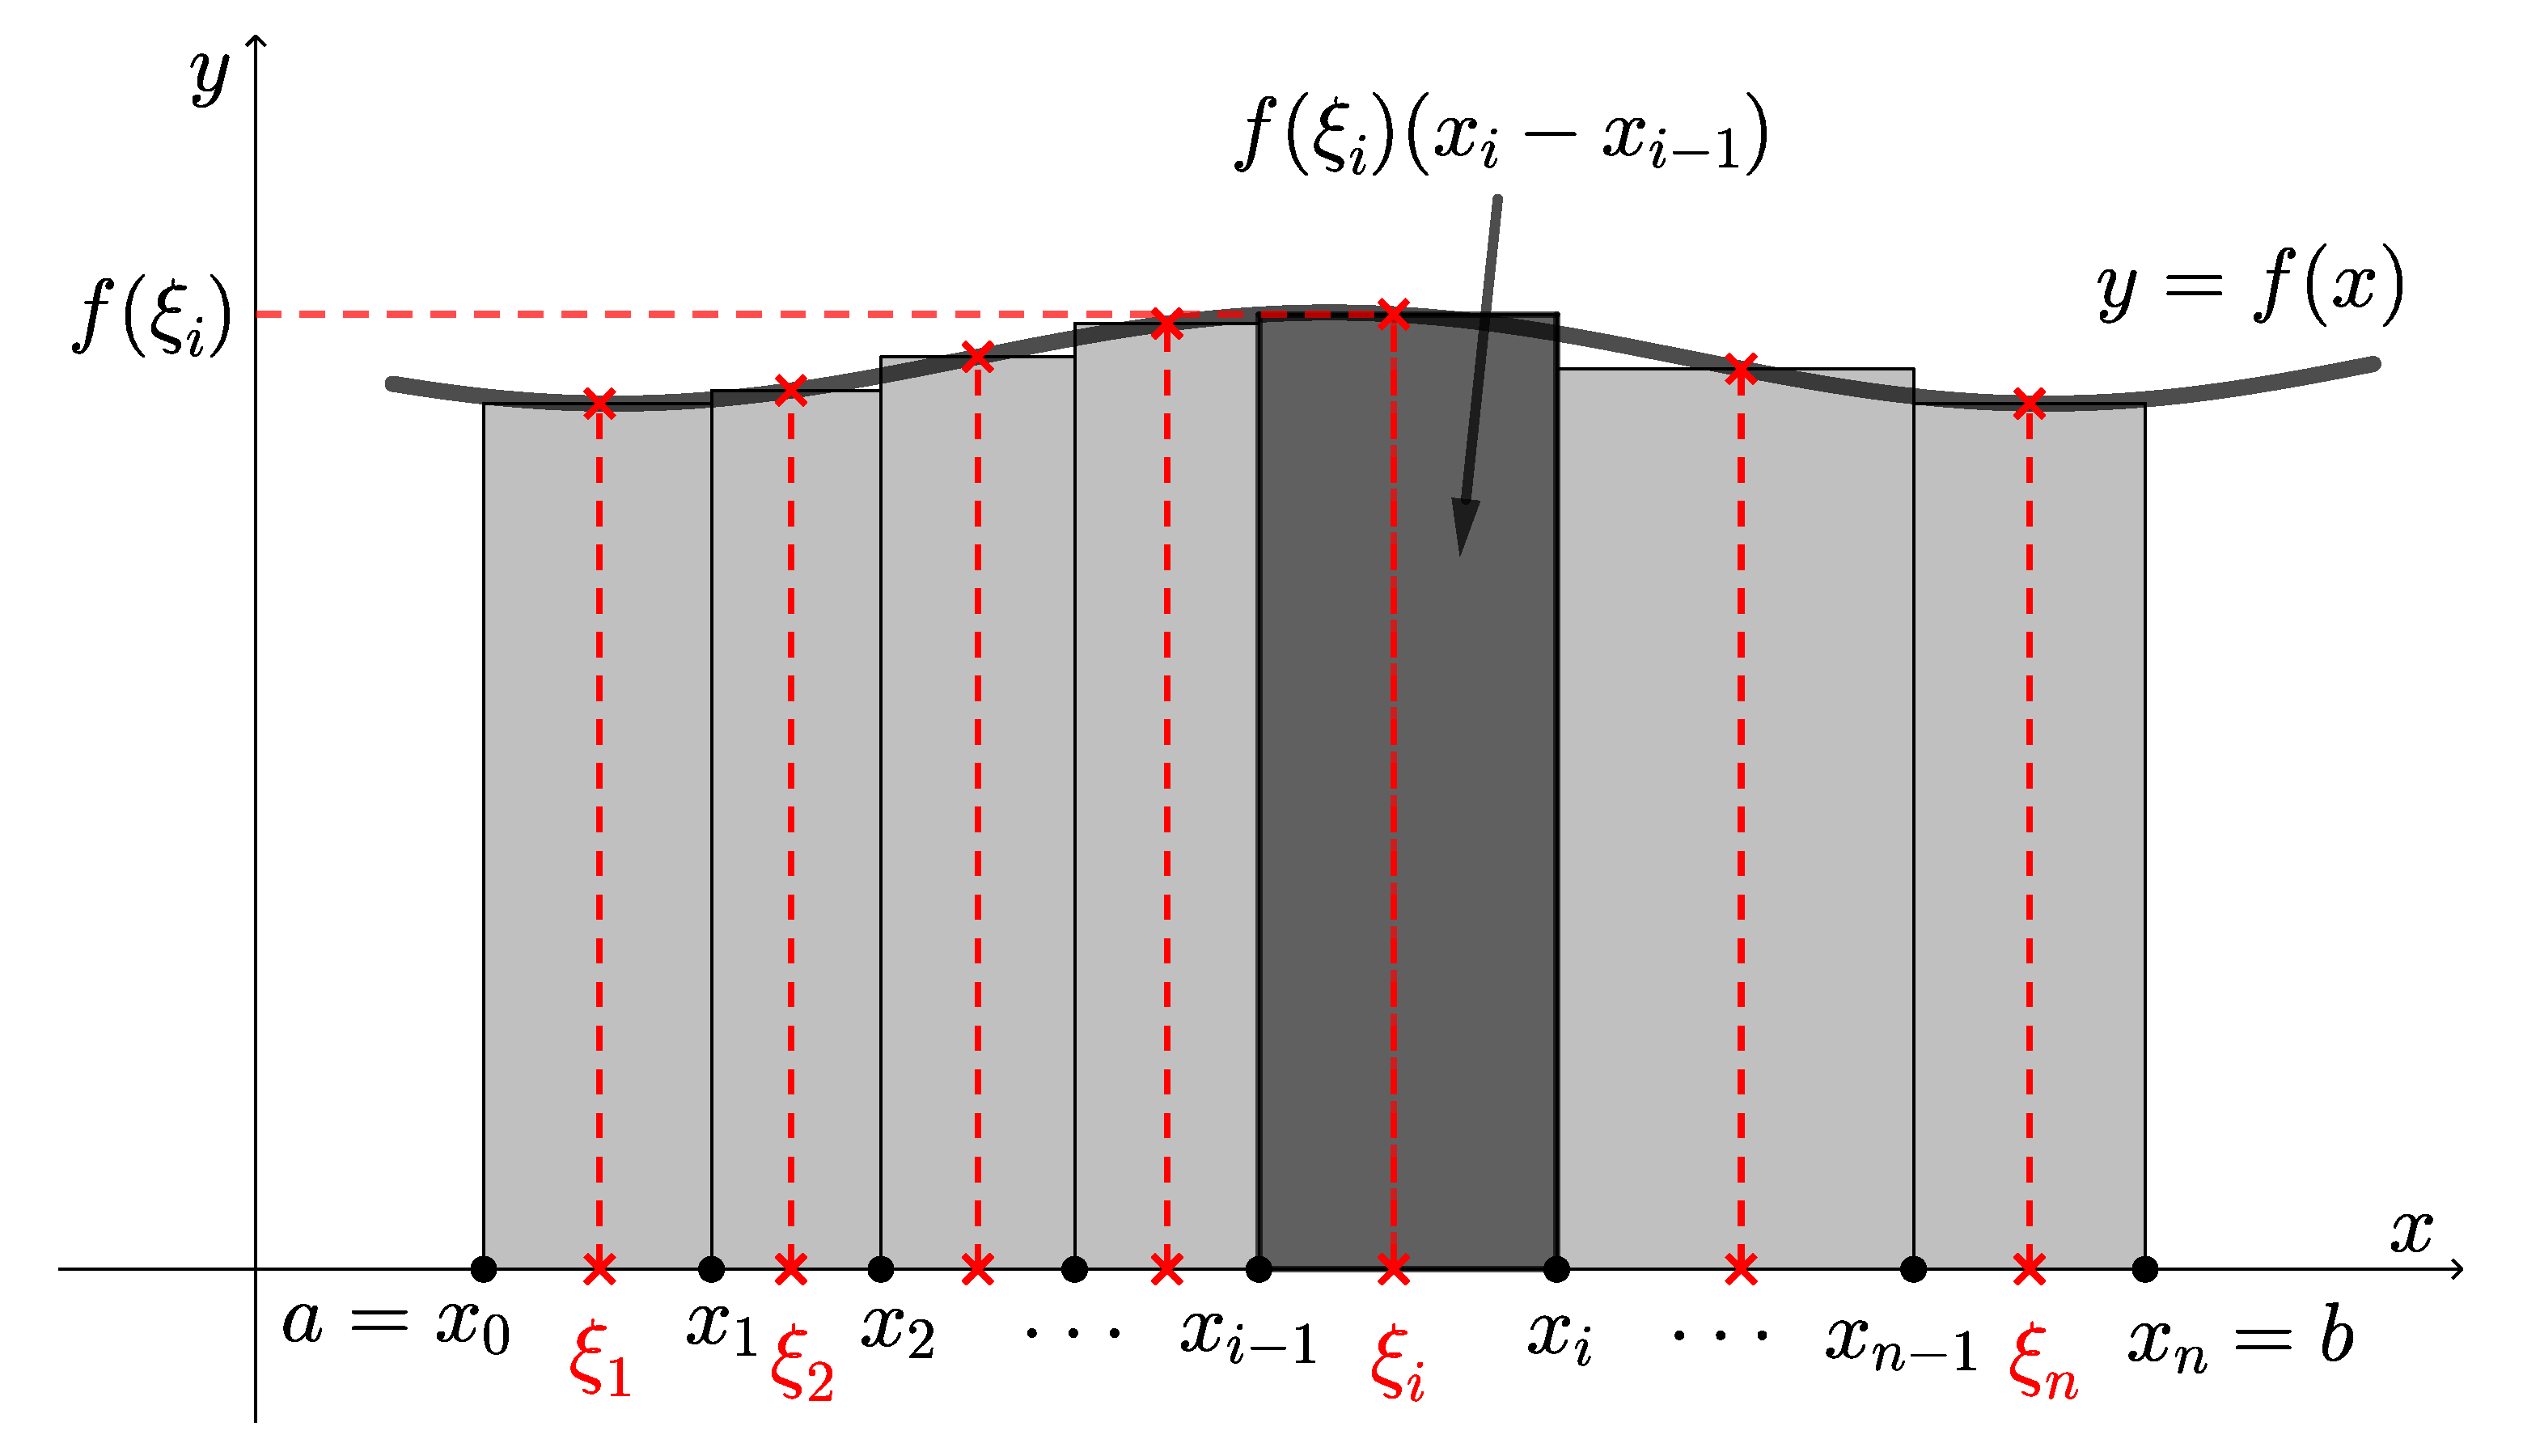
\includegraphics[height=6.5cm]{02/RiemannSum.pdf}
  \caption{Riemann 和 $\ds \sum_{i=1}^{n} f(\xi_i)(x_i-x_{i-1})$ は各長
    方形の(符号付き)面積の和に相当する. }\label{fig:RiemannSum1}
\end{figure}

\newpage

簡単な Riemann 和を実際に計算してみよう.

\begin{example}
  $f(x)=x^2$ とする.$\Delta=(x_0,x_1,x_2,x_3,x_4)$ を閉区
  間 $[0,4]$ の $4$ 等分割とし,各小区間 $[ x_{i-1}, x_{i}]$ の中点
  を $\xi_i$ とする.つまり,
  \[
    \Delta=(x_0, x_1, x_2, x_3, x_4) =(0,1,2,3,4), \quad
    \xi_1=\frac{1}{2}, \; \xi_2=\frac{3}{2}, \; \xi_3=\frac{5}{2}, \;
    \xi_4 = \frac{7}{2}
  \]
  とする.これらに関する $f$ の Riemann 和 $R(\Delta, \{\xi_i\}, f)$ を実際に計算してみよう.
  \[
    \begin{aligned}
      R\left( \Delta, \{\xi_i\}, f\right)
      &=f(\xi_1)(x_1-x_0)+f(\xi_2)(x_2-x_1) + f(\xi_3)(x_3-x_2) +
        f(\xi_4)(x_4-x_3)\\[2ex]
      &= f\left(\frac{1}{2}\right) \left( 1-0 \right) + f\left(\frac{3}{2}\right)\left(2-1\right)
        + f\left(\frac{5}{2}\right) \left(3-2\right) + f\left(\frac{7}{2}\right)\left(4-3\right)\\[2ex]
      & = \frac{1}{4} + \frac{9}{4} + \frac{25}{4} + \frac{49}{4} = 21
    \end{aligned}
  \]
\begin{figure}[h]
  \centering
  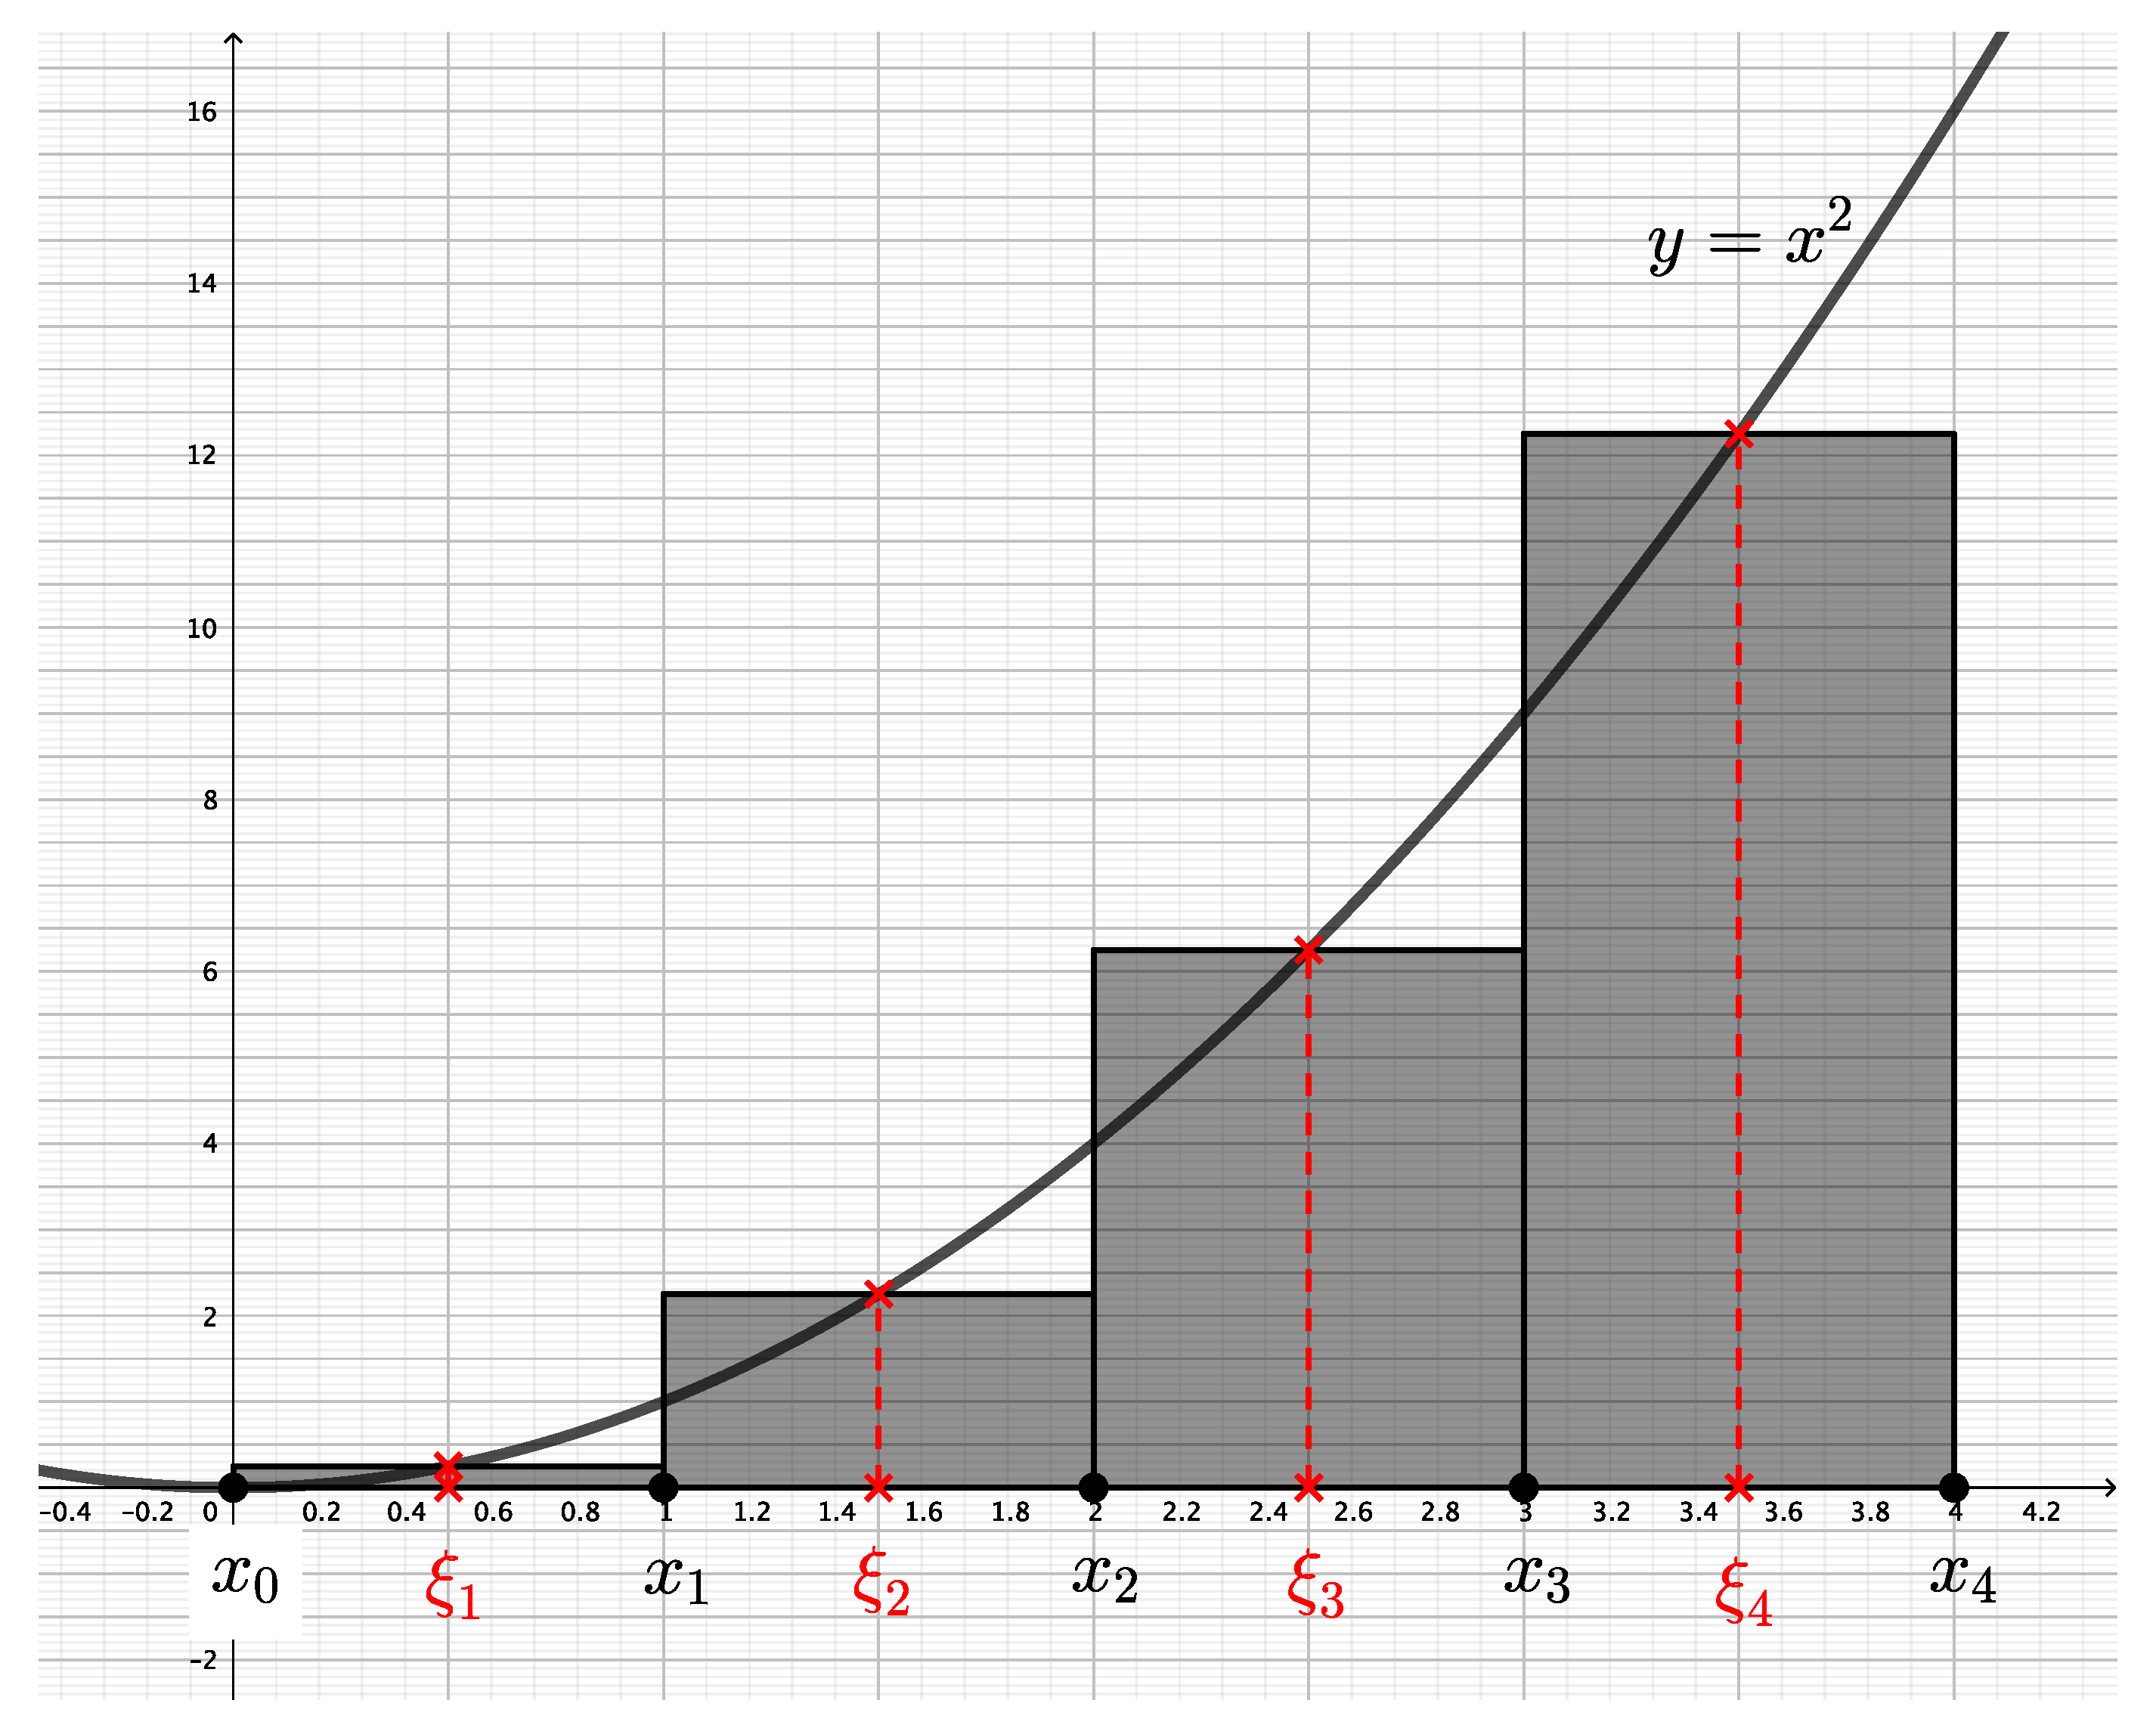
\includegraphics[height=12cm]{02/parabola.pdf}
\end{figure}

これは積分 $\ds \int_{0}^{4}x^2 \ dx $ を近似している.実際,後で確認す
るが $\ds \int_{0}^{4} x^2 \ dx = \frac{64}{3} = 21.333\cdots$ である.
\end{example}

\newpage


\subsection{積分の定義}

$f$ を有界閉区間 $[a,b]$ で有界な関数とする.$[a,b]$ の分
割 $\Delta =(x_0, \ldots, x_n)$ に対し,
\[
  |\Delta| := \max_{1 \leq i \leq n}(x_i - x_{i-1})
\]
とする.ここで,$\max$は最大値を意味する.すなわち,$x_1-x_0, x_2-x_1,
\ldots, x_{n}-x_{n-1}$ の中で最も大きな値が $|\Delta|$ であ
る.$|\Delta| \to 0$ のとき,分割の仕方と代表点集合 $\Set{\xi_i}$の選び
方によらず Riemann 和 $R(\Delta, \Set{\xi_i}, f)$ が一定の値に収束する
ならば,$f$ は $[a,b]$ で\textbf{(Riemann) 積分可能},また
は\textbf{(Riemann) 可積分}であるといい,その極限値を
\[
  \int_{a}^{b} f(x) \ dx
\]
で表し,区間 $[a,b]$ における $f$ の\textbf{積分}という.つまり,
\[
  \int_{a}^{b} f(x) \ dx = \lim_{|\Delta| \to 0} \sum_{i=1}^{n} f(\xi_i)(x_i-x_{i-1})
\]
である.ここまでは $a<b$ の場合しか想定していないが,$a \geqq b$ の場合も含めて以下を約束しておく.
\begin{equation}\label{eq:int_promis}
  \int_{a}^{b} f (x) \ dx = - \int_{b}^{a} f(x) \ dx, \qquad \int_{a}^{a} f(x) \ dx =0
\end{equation}


与えられた関数が積分可能であるかどうかを調べるのは容易ではないが,有界
閉区間上の連続関数は積分可能であることが知られている.

\begin{theorem}\label{thm:integrable1}
  有界閉区間 $[a,b]$ 上連続な関数は $[a,b]$ で積分可能である.
\end{theorem}

つまり,積分したい区間で $f$ が連続なら積分できるかどうかは心配する必要
がなく,「どうやって計算するか」のみ考をえればよい.\\

積分の定義から,以下の定理が成り立つ.

\begin{theorem}\label{thm:int_additive}
  $f$ の積分可能な範囲内にある任意の $a,b,c$ に対して以下が成り立つ.
  \[
    \int_{a}^{b} f(x) \ dx + \int_{b}^{c} f(x) \ dx = \int_{a}^{c} f(x) \ dx
  \]
\end{theorem}

\begin{theorem}\label{thm:int_monotomic}
  $f,g$ が区間 $[a,b]$ で積分可能かつ $f(x) \leqq g(x)$ なら $\ds \int_{a}^{b}f(x) \ dx \leqq \int_{a}^{b} g(x) \ dx$ である.
\end{theorem}

一般に,$- |f(x)| \leqq f(x) \leqq | f(x) |$ なので定理\ref{thm:int_monotomic}から以下が成り立つ.
\[
  -\int_{a}^{b} |f(x)| \ dx \leqq \int_{a}^{b} f(x) \ dx \leqq \int_{a}^{b} |f(x)| \ dx
\]
これにより,以下の定理が得られる.

\begin{theorem}\label{thm:int_absolute}
  $f$ が $[a,b]$ で積分可能なら $\ds \left| \int_{a}^{b} f(x) \ dx \right| \leqq \int_{a}^{b} |f(x)| \ dx$ である.
\end{theorem}

\subsection{微分積分学の基本定理}

積分値を定義に基づいて求めるのは大体困難であり,実際には微分積分学の基本定理を使って計算する.

\begin{theorem}[\textbf{微分積分学の基本定理}]\label{thm:fundamental}
  有界閉区間 $[a,b]$ 上の連続関数 $f$ に対して次が成り立つ.
  \begin{enumerate}[(1)]
  \item 関数 $\ds G(x) = \int_{a}^{x} f(t) \
    dt$ は閉区間 $[a,b]$ で定義され,開区間 $(a,b)$ で以下が成り立つ.
    \[
      G'(x)= f(x)
    \]
    つまり,$G$ は $f$ の原始関数である.
    
  \item $f$ の任意の原始関数 $F$ に対して(つまり,$F'=f$ となる任意の $F$ に対して)以下が成り立つ.
    \[
      \int_{a}^{b} f(x) \ dx = F(b) - F(a)
    \]
  \end{enumerate}
\end{theorem}

\begin{remark}
  この定理の(1)は,微分と積分という操作が互いに逆であることを示している.
  これがあるから「微分学」と「積分学」がまとめて「微分積分学」と呼ばれ
  ている.また,(2)は微分の逆操作によって実際に積分の値が計算できること
  を示している.この定理は微分積分学においてもっとも重要
  であり,だからこそ「基本定理」と呼ばれている.\\
\end{remark}

$F(b)-F(a)$ を $\Big[ F(x) \Big]_{a}^{b}$ と書くと便利である.これによって積分の計算は
\[
  \int_{a}^{b}f(x) \ dx = \Big[F(x)\Big]_{a}^{b} = F(a) - F(b) = \cdots 
\]
という形で書かれることが多い.\\

例えば,$\ds \left( \frac{x^3}{3} \right)' = x^3, \; \left( e^x \right)' = e^x$ なので
微分積分学の基本定理(2)から
\[
  \int_{0}^{4} x^2 \ dx = \left[ \frac{x^3}{3} \right]_{0}^{4} = \frac{4^3}{3} - \frac{0^3}{3} = \frac{64}{3}, \qquad
  \int_{0}^{1} e^x \ dx = \left[ e^x \right]_{0}^{1} = e^1 - e^0 = e-1
\]
などと積分の計算が容易に行える.とにかく,$F'=f$ となる $F$ さえ見つかれば積分は容易に計算できる.\\

また,$F'=f$ となる $F$
はどれを選んでもよい.例えば,$\ds \left( \log x \right)' = \left(
  \log (2x) \right)' = \frac{1}{x}$ なので
\[
  \int_{1}^{2} \frac{dx}{x} = \Big[ \log x \Big]_{1}^{2} = \log 2 - \log 1 = \log 2 \quad \Big( F(x) = \log x\Big)
\]
と計算しても
\[
  \int_{1}^{2} \frac{dx}{x} = \Big[\log(2x) \Big]_{1}^{2} = \log 4 - \log 2 = \log\frac{4}{2} = \log 2 \quad
  \Big( F(x) = \log (2x) \Big)
\]
と計算してもよい.ちなみに,$\log (2x) = \log x + \log 2$ なので,$\log x$ と $\log (2x)$ との差は定数 $\log 2$ である.

\subsection{定積分における部分積分と置換積分}

微分積分学の基本定理により,定積分 $\ds \int_{a}^{b} f(x) \ dx$ の計算
の大部分は実質不定積分 $\ds \int f(x) \ dx$ の計算である.そこに部分積分や
置換積分を適用する場合には積分範囲も含めて計算すればよい.\\

定積分で部分積分を適用する場合は,以下のように計算すればよい.
\[
  \int_{a}^{b} f(x)g'(x) \ dx = \Big[ f(x) g(x) \Big]_{a}^{b} - \int_{a}^{b} f'(x) g(x) \ dx
\]

\begin{example}

  \begin{enumerate}[(1)]
    \setlength{\itemsep}{1zh}
    
  \item $\ds \int_{0}^{1} x e^x \ dx = \Big[ x e^x \Big]_{0}^{1} - \int_{0}^{1} e^x \ dx = e -0 - \Big[ e^x \Big]_{0}^{1} =
    e - \left( e-1\right) = 1$

  \item
    $\ds \int_{1}^{2} x \log x \ dx = \left[ \frac{x^2}{2} \log x
    \right]_{1}^{2} - \int_{1}^{2} \frac{x}{2} \ dx = 2 \log 2 - 0 -
    \left[ \frac{x^2}{4} \right]_{1}^{2} = 2 \log 2 - \left( 1 -
      \frac{1}{4}\right) = 2 \log 2 - \frac{3}{4}$
  \end{enumerate}
  
\end{example}

\begin{remark}
  先に不定積分を計算しきってもよい.例えば,上の(1)で
  $\ds \int x e^x \ dx = x e^x - \int e^x \ dx = x e^x - e^x$ と不定積
  分を求めてしまってから以下のように計算してもよい.
  \[
    \int_{0}^{1} x e^x \ dx = \Big[ x e^x - e^x\Big]_{0}^{1} = (e-e) - (0 - 1) = 1
  \]
  これでももちろんよいが,$\ds \int$ が外れたところから代入計算をした方が早く結論に辿りつきやすい.\\
\end{remark}

定積分において,$u=g(x)$ として置換積分を適用する場合には,積分範囲も $u$ の動く範囲に変換する.
\[
  \int_{a}^{b} f\left( g(x) \right) \frac{du}{dx} \ dx = \int_{\alpha}^{\beta} f(u) \ du \quad \left[
    \begin{array}{c|ccc}
      x & a & \to & b \\ \hline
      u & \alpha & \to & \beta
    \end{array}
    \right]
\]

\begin{example}
  $\ds \int_{0}^{\pi/2} \frac{\cos x}{1+\sin x} \ dx$
  
  $u=1+\sin x$ とおくと $\ds \frac{du}{dx} = \cos x$ であり,積分範囲は $
  \begin{array}{c|ccc}
    x & 0 & \to & \pi/2 \\ \hline
    u & 1 & \to & 2
  \end{array}$ と変換される.
  \[
    \int_{0}^{\pi/2} \frac{\cos x}{1+\sin x} \ dx = \int_{0}^{\pi/2} \frac{1}{u}~ \frac{du}{dx} \ dx
    = \int_{1}^{2} \frac{du}{u} = \Big[ \log u \Big]_{1}^{2} = \log 2
  \]
\end{example}

\begin{remark}
  上の例で,先に不定積分を
  $\ds \int \frac{\cos x}{1+\sin x} \ dx = \int \frac{du}{u} = \log |u| = \log |1+\sin x|$ と計算しきってから
  \[
    \int_{0}^{\pi/2} \frac{\cos x}{1+\sin x} \ dx = \Big[ \log |1+\sin x| \Big]_{0}^{\pi/2}
    = \log 2 - \log 1 = \log 2
  \]
  と計算してももちろんよいが,積分範囲も変換しながら計算すれば,不定積分を計算しきる必要がなくなる.
\end{remark}


具体的な積分計算は以下のリンク先の「積分基本問題集 壱」(1) $\sim$ (26) で練習してください.
\begin{center}
  \url{https://github.com/kazutsumi/Integral1/blob/main/integral1.pdf}
\end{center}



\subsection{微分積分学の基本定理の証明}

微分積分学の基本定理(定理\ref{thm:fundamental})は微分積分学において最
も重要な定理なのでその証明を書いておく.興味がなければ読み飛ばしてもよ
い.なお,基本的に教科書と同じ証明である.

\begin{fundamental}
  有界閉区間 $[a,b]$ 上の連続関数 $f$ に対して次が成り立つ.
  \begin{enumerate}[(1)]
  \item 関数 $\ds G(x) = \int_{a}^{x} f(t)\ dt$ は閉区間 $[a,b]$ で定義され,開区間 $(a,b)$ で以下が成り立つ.
    \[
      G'(x) = f(x)
    \]
    
  \item $f$ の任意の原始関数 $F$ に対して以下が成り立つ.
    \[
      \int_{a}^{b} f(x) \ dx = F(b) - F(a)
    \]
  \end{enumerate}
\end{fundamental}

\vspace{1zh}

まず,(1)を認めてしまえば以下の補題\ref{lem:uptoC}から(2)は容易に示せる.

\begin{lemma}\label{lem:uptoC}
  $F,G$ を有界閉区間 $[a,b]$ 上の連続関数 $f$ の原始関数とする.このと
  き,$F(x) = G(x) +C$ となる定数 $C$ が存在する.
\end{lemma}

\begin{proof}
  $H(x) = F(x) - G(x)$ とする.$H'(x) = F'(x) - G'(x) = f(x) - f(x) =
  0$ なので,$H$ は $[a,b]$ 上の定数関数である.実際,平均値の定理から
  任意の $x_1 ,x_2 \in [a,b] \; ( x_1 < x_2)$ に対して
  \[
    \frac{H(x_2) - H(x_1)}{x_2-x_1} = H'(c) , \quad x_1 < c < x_2
  \]
  となる実数 $c$ が存在するが,$H'(c)=0$ なので $H(x_1) =
  H(x_2)$ より $H$ は定数関数である.よって,$H(x) = F(x) - G(x) = C$
  となる定数 $C$ が存在する.これより,$F(x) = G(x) +C$ である.
\end{proof}

\vspace{1zh}

\begin{proof}[微分積分学の基本定理(2)の証明]
  (1)から $G(x)$ は $f$ の原始関数なので,補
  題\ref{lem:uptoC}から $F(x) = G(x) +C$ を満たす定数 $C$ が存在する.
  また,$\ds \int_{a}^{a} f(t) \ dt =0$ と約束しているので
  \[
    F(b) - F(a) = \Big(G(b) +C \Big) - \Big(G(a) +C\Big) = G(b) - G(a)
    = \int_{a}^{b} f(t) \ dt - \int_{a}^{a} f(t) \ dt = \int_{a}^{b} f(x) \ dx
  \]
  である.なお,変数に使う文字によって積分値は変わらないので
  $\ds \int_{a}^{b} f(t) \ dt = \int_{a}^{b} f(x) \ dx$ である.
\end{proof}

\newpage

次に,定理\ref{thm:int_additive}と以下の補題\ref{lem:int_average}から微分積分学の基本定理(1)を証明する.

\begin{lemma}[\textbf{積分の平均値の定理}]\label{lem:int_average}
  有界閉区間 $[a,b]$ 上の連続関数 $f$ に対し,以下を満たす実数 $c$ が存在する.
  \[
    \int_{a}^{b}f(x) \ dx = f(c)(b-a), \quad a < c < b
  \]
\end{lemma}

\begin{proof}
  $f$ が定数関数なら明らかなので,$f$ は定数関数でないとする.$f$ は閉
  区間 $[a,b]$ で連続なので最小値 $m$ と最大値 $M$ が存在する.それらを
  実現する値をそれぞれ $x_{\min}, x_{\max} \in [a,b]$ とする.つま
  り,$f(x_{\min})=m, \; f(x_{\max})=M$ である.$f$ は定数関数でないの
  で $x_{\min} \neq x_{\max}$ である.定理\ref{thm:int_monotomic}より
  \[
    m(b-a) = \int_{a}^{b} m \ dx \leqq \int_{a}^{b} f(x) \ dx \leqq \int_{a}^{b} M \ dx = M (b-a)
  \]
  が成り立つ.これより
  \[
    m \leqq \frac{1}{b-a} \int_{a}^{b} f(x) \ dx \leqq M
  \]
  である.よって,中間値の定理から
  \[
    \frac{1}{b-a} \int_{a}^{b} f(x) \ dx = f(c), \quad x_{\min} < c < x_{\max} \text{ または } x_{\max} < c < x_{\min}
  \]
  を満たす実数 $c$ が存在する.従って,
  \[
    \int_{a}^{b} f(x) \ dx = f(c) (b-a)
  \]
  である.ここで,$x_{\min}, x_{\max} \in [a,b]$ なので $a < c < b$ である.
\end{proof}

\vspace{1zh}

\begin{proof}[微分積分学の定理(1)の証明]
  $x \in (a,b)$ とする.定理\ref{thm:int_additive}と約束 (\ref{eq:int_promis}) から
  \[
    \begin{aligned}
      \frac{G(x+h) - G(x)}{h}
      &= \frac{1}{h}\left(\int_{a}^{x+h}f(t) \ dt - \int_{a}^{x} f(t) \ dt\right)
        \underset{(\ref{eq:int_promis})}{=}\frac{1}{h} \left( \int_{a}^{x+h} f(t) \ dt + \int_{x}^{a} f(t) \ dt \right)\\
      &\underset{\text{定理\ref{thm:int_additive}}}{=} \frac{1}{h} \int_{x}^{x+h} f(t) \ dt
    \end{aligned}
  \]
  である.さらに,補題\ref{lem:int_average}から
  \[
    \int_{x}^{x+h} f(t) \ dt = f(c)h
  \]
  を満たす実数 $c$ が $x$ と $x+h$ の間に存在するので
  \[
    \frac{G(x+h) - G(x)}{h} = f(c)
  \]
  である.$h \to 0$ のとき $c \to x$ であり,$f$ は連続なので
  \[
    G'(x) = \lim_{h \to 0} \frac{G(x+h)-G(x)}{h} = \lim_{c \to x} f(c) = f(x)
  \]
  である.つまり,$G$ は開区間 $(a,b)$ で微分可能で $G'(x) = f(x)$ である.
\end{proof}
\newpage

\subsection{(おまけ)Riemann 和の極限としての積分}\label{sec:Rsum_computation}
有界閉区間上の連続関数の積分の値を Riemann 和の極限としていくつか計算する.

\begin{example}
$\ds \int_{0}^{4} x^2 \ dx$ 

  \vspace{1zh}

  $\Delta_n=(x_0, \ldots, x_n)$ を閉区間 $[0,4]$ の $n$ 等分割,各小区間 $[x_{i-1}, x_i]$
  の中点を代表点 $\xi_i$ とする.つまり,
  \[
    x_i = \frac{4i}{n} \; (i=0,1, \ldots, n) , \qquad \xi_i =
    \frac{x_{i-1} + x_{i}}{2} = \frac{2(2i-1)}{n} \; (i=1,2, \ldots, n)
  \]
  とする.これらに関する $f(x) =
  x^2$ の Riemann 和を $S_n$ とする.これは図\ref{fig:Rsum_quadratic}の灰色部分の面
  積に等しい.
  \begin{figure}[h]
    \centering
    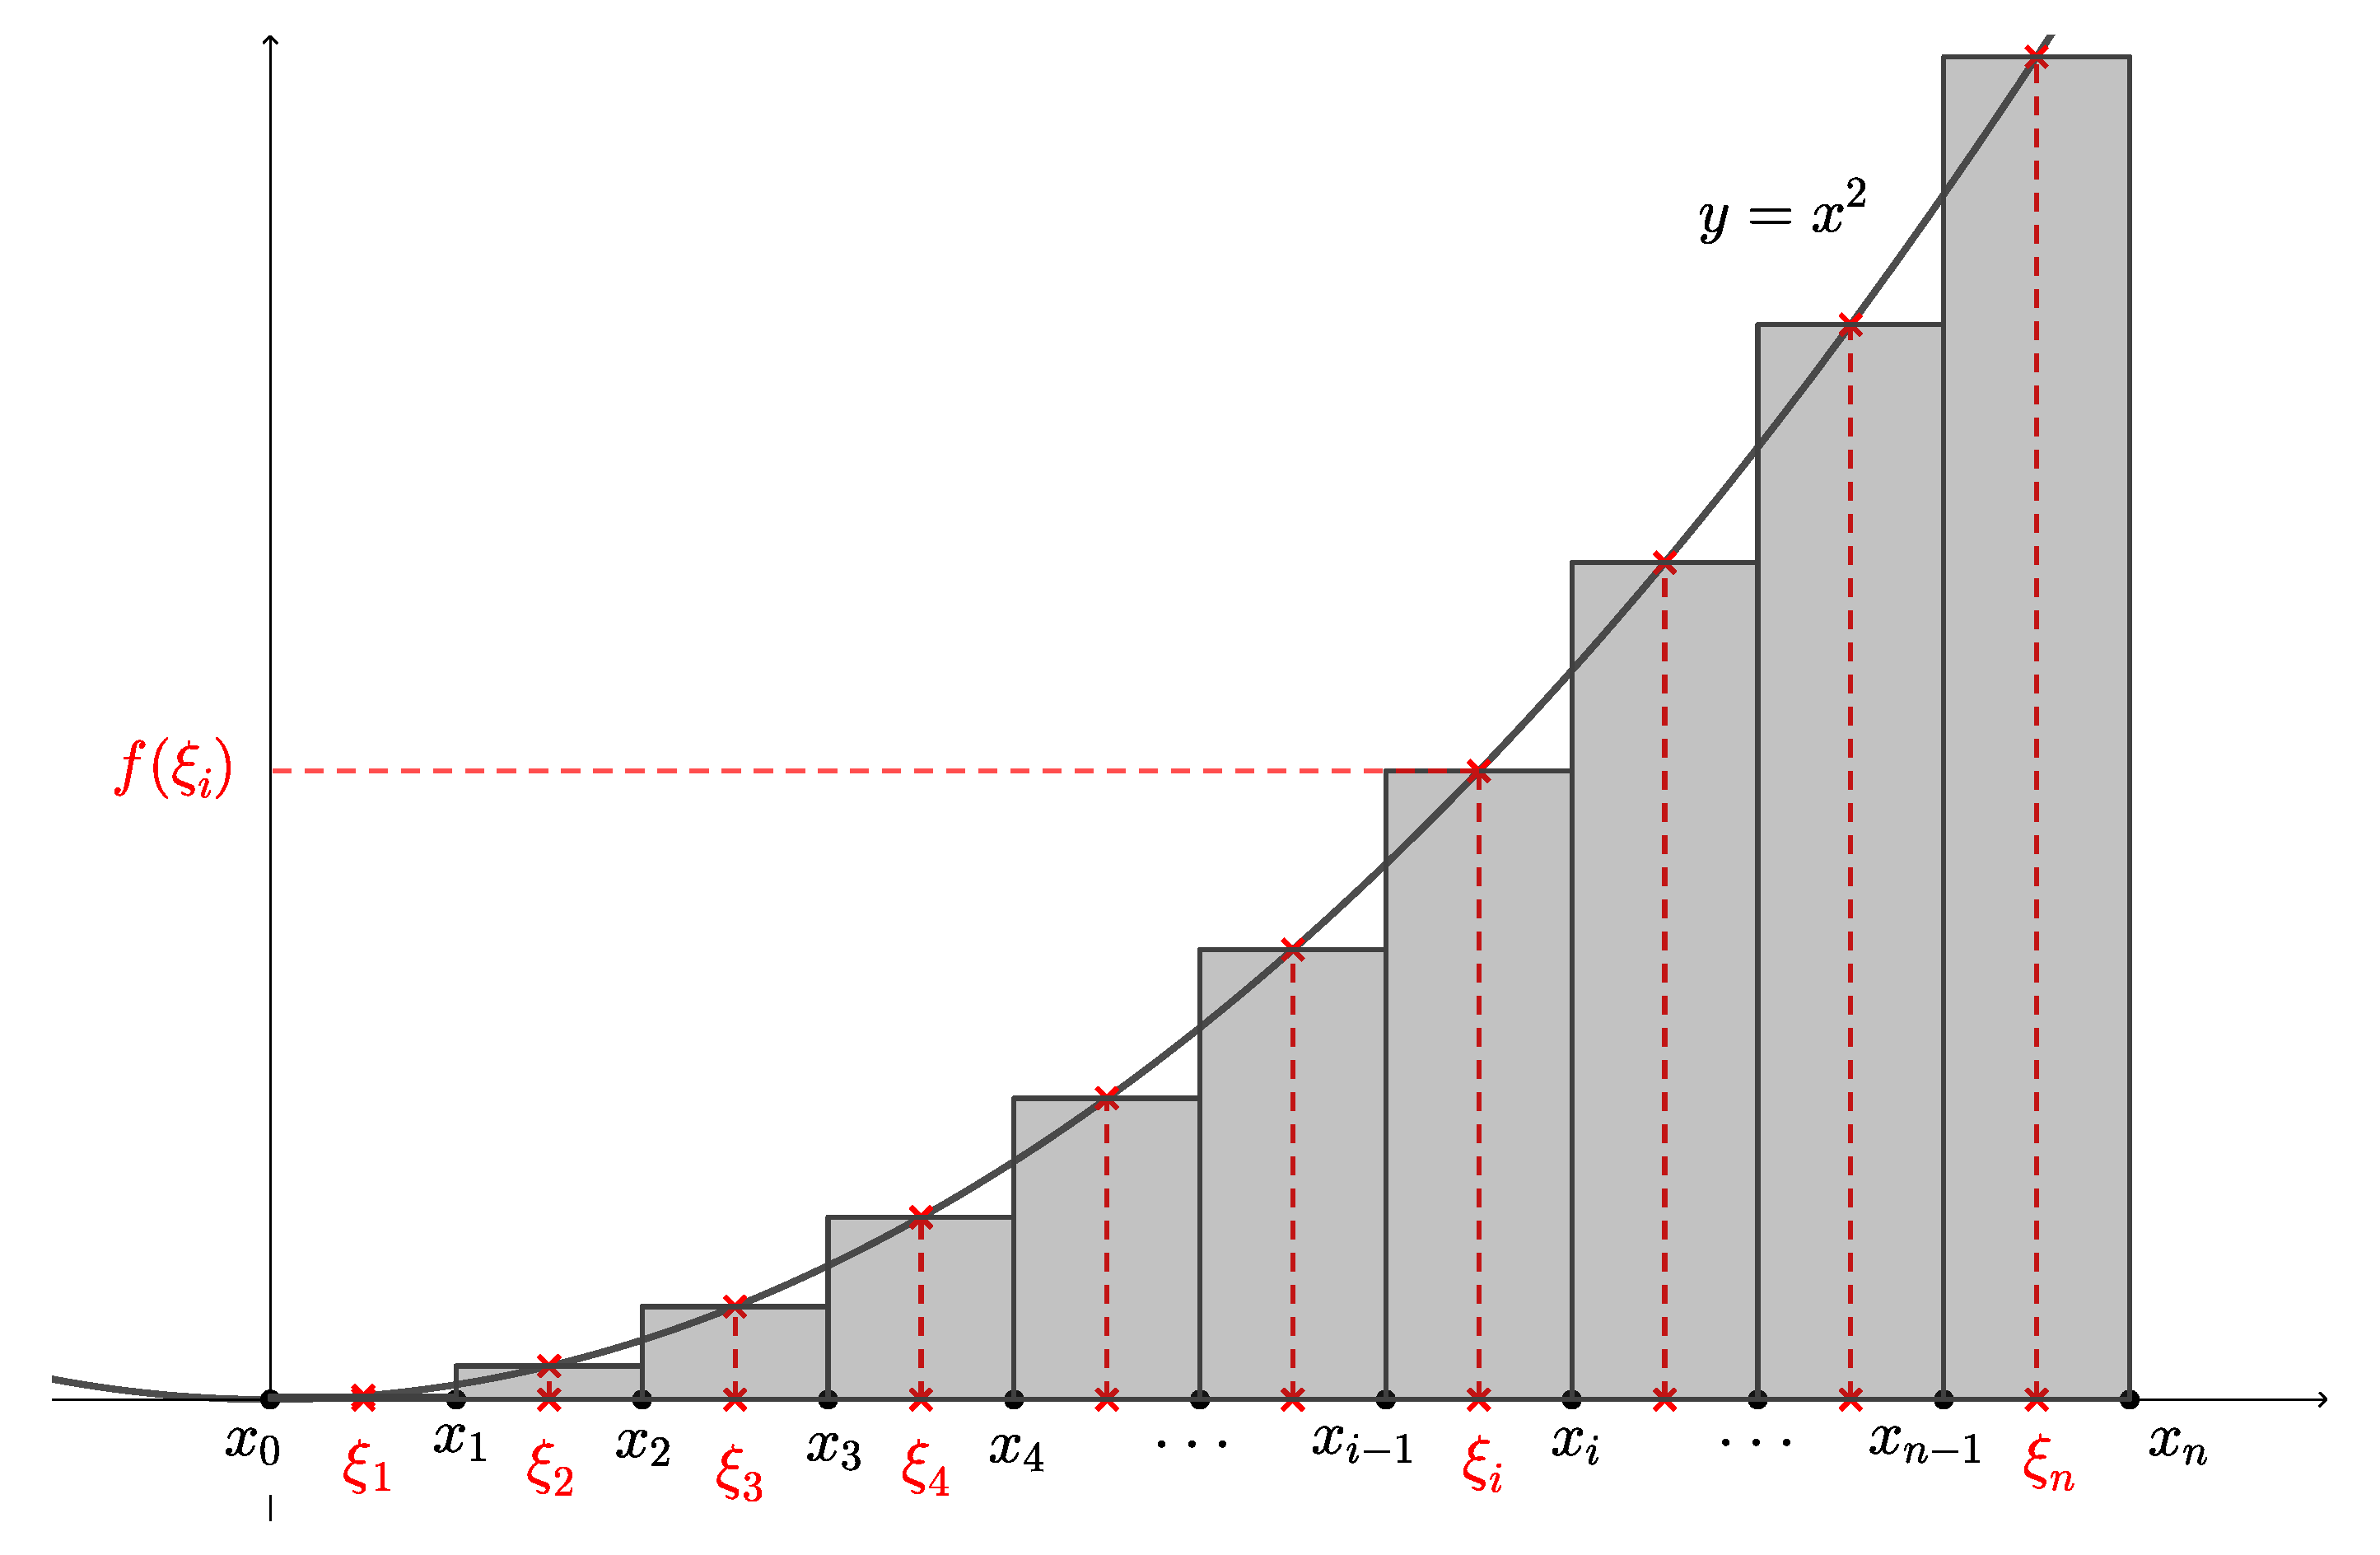
\includegraphics[height=8cm]{02/quadratic.pdf}
    \caption{}\label{fig:Rsum_quadratic}
  \end{figure}
  $n \to \infty$ のとき,$|\Delta_n| \to 0$ だから定理\ref{thm:integrable1}より $S_n$ は
  収束し,その極限値が求める積分値である.

  Riemann 和 $\ds S_n $ を具体的に計算する.$\Delta_n$ は区間 $[0,4]$ の $n$ 等
  分割なので,各 $i$ で $\ds x_{i} - x_{i-1} = \frac{4}{n}$ である.
  \[
    \begin{aligned}
      S_n &= \sum_{i=1}^{n} f(\xi_i)(x_i - x_{i-1})
            = \sum_{i=1}^{n} \left( \frac{2(2i-1)}{n}\right)^2 \cdot \frac{4}{n}
            =\frac{16}{n^3}\sum_{i=1}^{n} (2i-1)^2
            = \frac{16}{n^3} \sum_{i=1}^{n} \left(4i^2-4i+1\right)\\[2ex]
          &  = \frac{16}{n^3} \left( 4 \sum_{i=1}^{n} i^2 - 4 \sum_{i=1}^{n} i + \sum_{i=1}^{n} 1\right)
            = \frac{16}{n^3} \left( 4 \cdot \frac{n(n+1)(2n+1)}{6} - 4 \cdot \frac{n(n+1)}{2} + n\right)\\[2ex]
          &= 16 \left( \frac{2}{3} \left( 1 + \frac{1}{n}\right)\left(2+\frac{1}{n}\right)
            - \frac{2}{n} \left(1+\frac{1}{n}\right) + \frac{1}{n^2}\right) \to \frac{64}{3} \; (n \to \infty)
    \end{aligned}
  \]
  これより,$\ds \int_{0}^{4}x^2 \ dx = \lim_{n \to \infty} S_n = \frac{64}{3}$ である.
\end{example}

\newpage

\begin{example}
  $\ds \int_{0}^{1} e^x \ dx$ 

  \vspace{1zh}
  
  $\Delta_n=(x_0,\ldots, x_n)$ を閉区間 $[0,1]$ の $n$ 等分割,各小区間 $[x_{i-1},x_i]$ の
  右端 $x_i$ を代表点 $\xi_i$ とする.つまり,
  \[
    x_i = \xi_i = \frac{i}{n}
  \]
  とする.これらに関する $f(x) = e^x$ の Riemann和を $S_n$ とする.こ
  れは図\ref{fig:Rsum_exp}の灰色部分の面積に等しい.$n \to \infty$ のと
  き,$|\Delta_n| \to 0$ だから定理\ref{thm:integrable1}より $S_n$ は収束し,その極限値が求める積分
  値である.
  \begin{figure}[h]
    \centering
    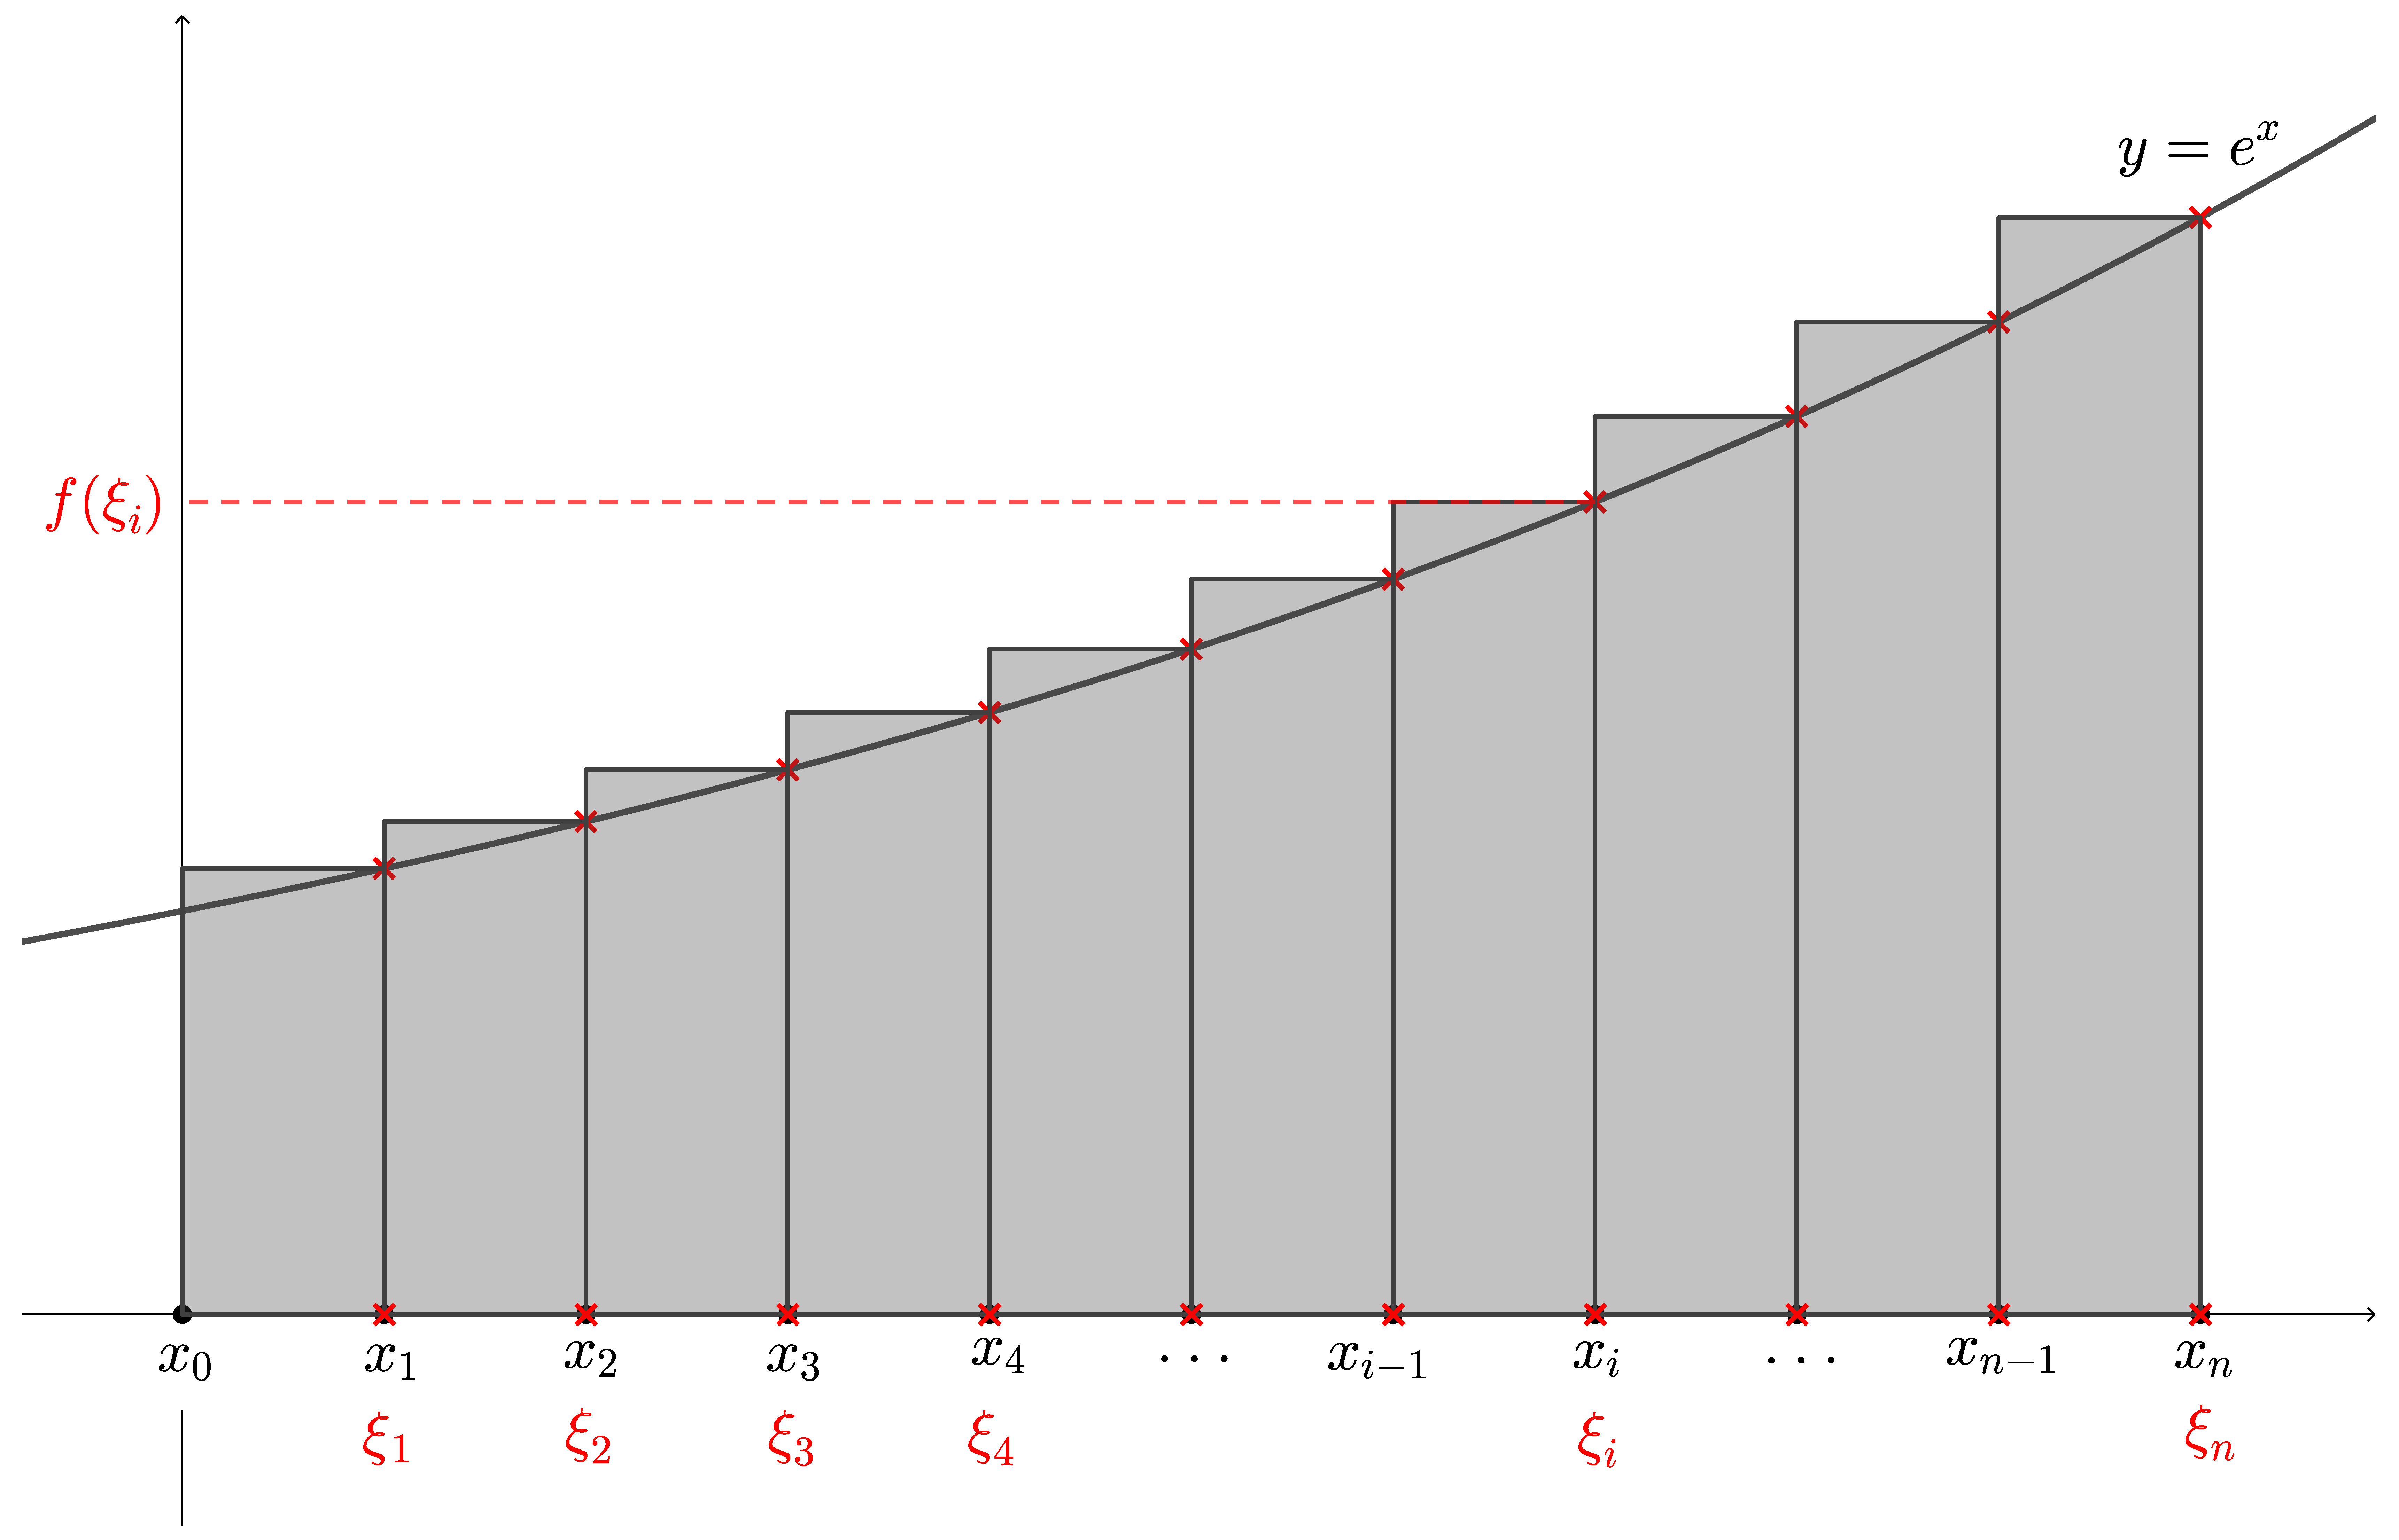
\includegraphics[height=8cm]{02/exp.pdf}
    \caption{}\label{fig:Rsum_exp}
  \end{figure}
\end{example}

Riemann 和 $S_n$ を具体的に計算する.$\Delta_n$ は区間 $[0,1]$ の $n$ 等分割な
ので,各 $i$ で $\ds x_i-x_{i-1} = \frac{1}{n}$ である.
\[
  \begin{aligned}
    S_n &= \sum_{i=1}^{n} f(\xi_i) (x_i-x_{i-1}) = \sum_{i=1}^{n} e^{\frac{i}{n}} \cdot \frac{1}{n}\\[2ex]
        & = \frac{1}{n} \left( e^{\frac{1}{n}}
          + \left(e^{\frac{1}{n}}\right)^2 + \left( e^{\frac{1}{n}}\right)^3 +\cdots
          + \left( e^{\frac{1}{n}}\right)^n\right) \quad \left( \text{ 公比 $e^{\frac{1}{n}}$ の等比級数}\right)\\[2ex]
        & = \frac{1}{n} \cdot \frac{e^{\frac{1}{n}} \left( 1 - \left( e^{\frac{1}{n}}\right)^n\right)}{1-e^{\frac{1}{n}}}
          = \frac{e^{\frac{1}{n}}}{n} \cdot \frac{e-1}{e^{\frac{1}{n}}-1}
  \end{aligned}
\]
ここで,$\ds t=e^{\frac{1}{n}}-1$ とおく.これにより $\ds \frac{1}{n} = \log(1+t)$ なので,
\[
  S_n = \frac{\log(1+t)}{t} \cdot (e-1)(t+1) = (e-1) (t+1) \log(1+t)^{\frac{1}{t}}
\]
と変形できる.$n \to \infty$ のとき $t \to +0$ なので,$\ds \lim_{t \to +0} \log (1+t)^{\frac{1}{t}}=1$ と合わせて以下を得る.
\[
  \int_{0}^{1} e^x \ dx = \lim_{n \to \infty} S_n = (e-1) \lim_{t\to +0} (t+1) \log (1+t)^{\frac{1}{t}} = e-1
\]


定数関数 $f(x) = C$ は連続関数だが,定理\ref{thm:integrable1}に頼ることなく直接積分を計算できる.
\begin{example}
  $\ds \int_{a}^{b} C \ dx$\\

  $\Delta = (x_0, \ldots, x_n)$ を閉区間 $[a,b]$ の任意の分割とし,各小
  区間の $[x_{i-1}, x_{i}]$ の代表点 $\xi_i$ を任意に選ぶ.これらに関す
  る $f(x) = C$ の Riemann 和は
  \[
    \begin{aligned}
      R(\Delta, \{\xi_i\}, f) &= \sum_{i=1}^{n} f(\xi_i) (x_i - x_{i-1}) = \sum_{i=1}^{n} C (x_{i}-x_{i-1})\\[2ex]
                              & = C \Big( (x_1-x_0) + (x_2-x_1) + \cdots + (x_n-x_{n-1}) \Big)
                                = C(x_n-x_0) = C(b-a)
    \end{aligned}
  \]
  である.よって,分割の仕方と代表点の選び方によらず Riemann 和は一定な
  ので,特に $|\Delta|\to 0$ における極限値もその一定の値に等しい.よっ
  て,$\ds \int_{a}^{b} C \ dx = \lim_{|\Delta| \to 0} R(\Delta, \{\xi_i\}, f) = C(b-a)$ である.
\end{example}



\end{document}


\documentclass[10pt, uplatex, dvipdfmx]{jsarticle}
\usepackage{../mypackage}

\graphicspath{{../pictures}}

\setcounter{section}{2}

\begin{document}


\section{分数関数の積分}

$\ds \frac{\text{多項式}}{\text{多項式}}$ という形をした関数
は\textbf{分数関数}とか\textbf{有理関数}と呼ばれる.その積分の計算方法をまとめる.
% \[
%   \int \frac{dx}{(x-\alpha)^n}, \qquad \int \frac{Bx+C}{(x^2+bx+c)^n}\ dx
%   \qquad (n \text{ は自然数 })
% \]

\subsection{多項式の割り算}\label{subsec:division}

\begin{wrapfigure}{r}[0pt]{0.5\textwidth}
  \centering
  \includegraphics[width=7cm]{03/remainder.pdf}
\end{wrapfigure}
例えば,次のような分数関数 $f(x)$ を積分したい.
\[
  f(x) = \frac{x^5+3x^3-2x+1}{x^2+3x+2}
\]
この分子と分母の多項式としての次数を比べると
\[
  \text{ 分子の次数 }  \geqq \text{ 分母の次数} 
\]
である.このような場合は,まず右のように分子を分母で割った商と余
りを計算しておく.この計算により $f(x)$ の分子が
\[
  x^5+3x^3-2x+1 = (x^3-3x^2+10x-24)(x^2+3x+2) + 50x+49
\]
と書けるので
\[
  f(x) = \frac{ (x^3-3x^2+10x-24)(x^2+3x+2) + 50x+49}{x^2+3x+2} = x^3-3x^2+10x-24 + \frac{50x+49}{x^2+3x+2}
\]
と変形できる.よって,$f(x)$ の積分は
\[
  \int f(x) \ dx = \frac{1}{4}x^4 - x^3-5x^2-24x + \int
  \frac{50x+49}{x^2+3x+2} \ dx
\]
となり,もともとの $\ds \frac{\text{ $5$ 次式}}{\text{ $2$ 次式}}$ の積
分が $\ds \frac{\text{$1$ 次式}}{\text{$2$ 次式}}$ の積分に帰着されている.より一般に,分数関数が
\[
  f(x) = \frac{g(x)}{h(x)}
\]
と,$2$ 個の多項式 $g(x)$ と $h(x)$ の比で書けるとき,多項式の割り算を実行して
\[
  g(x) = q(x) h(x) + r(x), \quad \deg r(x) < \deg h(x)
\]
を満たす多項式 $q(x)$ と $r(x)$ を計算することができる.$q(x)$ が商
で,$r(x)$ が余りである.ただし,初めから $\deg g(x) < \deg h(x)$ であ
れば,$q(x)=0, \; r(x) = h(x)$ である.これらによって
\[
  f(x) = \frac{q(x)h(x)+r(x)}{h(x)} = q(x) + \frac{r(x)}{h(x)}
\]
と,$f(x)$ を「多項式」と「分子の次数 $<$ 分母の次数となる分数関数」の和に分けることができる.つまり,
\[
  \text{ 分子の次数 } < \text{ 分母の次数}
\]
となる分数関数の積分が計算できれば,原理的にはどんな分数関数の積分も計算できる.

\subsection{部分分数分解}\label{subsec:partfrac}

分数関数 $\ds f(x) = \frac{x^5+3x^2-2x+1}{x^2+3x+2}$ の積分を完成させよう.先ほど見たように
\[
  \int f(x) \ dx = \frac{1}{4}x^4-x^3-5x^2-24x + \int \frac{50x+49}{x^2+3x+2} \ dx
\]
なので,最後に残った積分
\[
  \int \frac{50x+49}{x^2+3x+2}\ dx
\]
を計算してしまえばよい.まず,分母が
\[
  \frac{50x+49}{x^2+3x+2} = \frac{50x+49}{(x+1)(x+2)}
\]
と因数分解できる.これをさらに
\[
  \frac{50x+49}{(x+1)(x+2)} = \frac{A}{x+1} + \frac{B}{x+2}
\]
という簡素な分数関数の和に分けることができる.特に,左辺が
\[
  \text{ 分子の次数 } < \text{ 分母の次数}
\]
なので,右辺に並ぶ分数関数も全てそうなる.従って,$A, B$ は共に $0$ 次,つまり定数である.実際,
上式の右辺を通分すれば
\[
  \frac{A}{x+1} + \frac{B}{x+2} = \frac{A(x+2)+B(x+1)}{(x+1)(x+2)} = \frac{(A+B)x + (2A+B)}{(x+1)(x+2)}
\]
となるので,分子の係数を比較して以下の連立1次方程式を解けばよい.
\[
  \begin{cases}
    A+B=50\\
    2A+B=49
  \end{cases} \quad \left( \Longleftrightarrow \left[
      \begin{array}{rr}
        1 & 1\\
        2 & 1
      \end{array}
      \right] \left[
        \begin{array}{r}
          A\\
          B
        \end{array}
      \right] = \left[
        \begin{array}{r}
          50\\
          49
        \end{array}
      \right] \right)
\]
これは簡単に解けて,$A=-1, \; B=51$ である. つまり,
\[
  \frac{50x+49}{(x+1)(x+2)} = -\frac{1}{x+1} + \frac{51}{x+2}
\]
なのでその積分は
\[
  \int \frac{50x+49}{(x+1)(x+2)} \ dx = -\int\frac{dx}{x+1} + 51\int
  \frac{dx}{x+2}= -\log|x+1| +51\log|x+2|
\]
と計算できる.これによって,$f(x)$ の積分が以下の通り完成する.
\[
  \int \frac{x^5+3x^2-2x+1}{x^2+3x+2} \ dx = \frac{1}{4}x^4 -
  x^3-5x^2-24x -\log|x+1| + 51 \log |x+2|
\]

\newpage

別の例として,次の分数関数 $g(x)$ を積分してみよう.
\[
  g(x) = \frac{6x^2+x+1}{x^3+x^2+x+1}
\]
これは初めから
\[
  \text{ 分子の次数 } < \text{ 分母の次数}
\]
なので,多項式の割り算を実行する必要はない.分母が
\[
  x^3+x^2+x+1 = x^2(x+1) + x+1 = (x^2+1)(x+1)
\]
と因数分解できるので,$g(x)$ を次の形に分解する.
\[
  \frac{6x^2+x+1}{(x+1)(x^2+1)} = \frac{\bigcirc}{x+1} + \frac{\square}{x^2+1}
\]
右辺はどちらも「分子の次数 $<$ 分母の次数」としたいの
で,$\bigcirc$ は定数($0$ 次)で,$\square$ は $1$ 次以下の多項式である.そ
こで,$\bigcirc = A, \; \square = Bx+C$ とおく.つまり,以下を満たす定数 $A,B,C$ を見つければよい.
\[
  \frac{6x^2+x+1}{(x+1)(x^2+1)} = \frac{A}{x+1} + \frac{Bx+C}{x^2+1}
\]
結果的にもしも $B=0$ となれば $\square$ は定数だったことになるが,それは計算
してみないとわからないので,とりあえずは $\square$ を $1$ 次式としておく.上式の右辺を通分すれば
\[
  \frac{6x^2+x+1}{(x+1)(x^2+1)} = \frac{A(x^2+1) +
    (x+1)(Bx+C)}{(x+1)(x^2+1)} = \frac{(A+B)x^2 + (B+C)x +
    (A+C)}{(x+1)(x^2+1)}
\]
となるので,分子の係数を比較して以下の連立1次方程式を解けばよい.
\[
  \begin{cases}
    A+B=6\\
    B+C=1\\
    A+C=1
  \end{cases} \quad \left( \Longleftrightarrow \left[
      \begin{array}{rrr}
        1 & 1 & 0\\
        0 & 1 & 1\\
        1 & 0 & 1
      \end{array}
    \right]\left[
      \begin{array}{r}
        A\\
        B\\
        C
      \end{array}
    \right] = \left[
      \begin{array}{r}
        6\\
        1\\
        1
      \end{array}
    \right]
  \right)
\]
これは簡単に解けて,$A=3, \; B=3, \; C=-2$ である.つまり,
\[
  g(x) = \frac{6x^2+x+1}{(x+1)(x^2+1)} = \frac{3}{x+1} + \frac{3x-2}{x^2+1}
\]
なので,その積分は以下のように計算できる.
\[
  \begin{aligned}
    \int g(x) \ dx
    &= 3\int \frac{dx}{x+1} + 3\int \frac{x}{x^2+1} \ dx - 2 \int \frac{dx}{x^2+1}\\[1ex]
    &  =3\log|x+1| + \frac{3}{2}\int \frac{2x}{x^2+1}\ dx - 2 \tan^{-1}x\\[1ex]
    &= 3\log|x+1| + \frac{3}{2} \int \frac{(x^2+1)'}{x^2+1}\ dx - 2\tan^{-1}x\\[1ex]
    &  =3 \log|x+1| + \frac{3}{2} \log(x^2+1) -2\tan^{-1}x 
  \end{aligned}
\]

\newpage

より一般に,分数関数 $\ds \frac{Q(x)}{P(x)}$の分母が互いに素な $r$ 個の多項式の積として
\[
  P(x) = P_1(x)P_2(x) \cdots P_r(x)
\]
と因数分解されれば,分数関数を多項式 $Q_0(x)$ といくつかの分数関数の和として
\[
  \frac{Q(x)}{P(x)} = Q_0(x) + \frac{Q_1(x)}{P_1(x)} + \frac{Q_2(x)}{P_2(x)} +
  \cdots + \frac{Q_r(x)}{P_r(x)} \quad (\deg Q_i(x) < \deg P_i(x), \; i=1,2, \ldots, r)
\]
となるように分解できる.これを分数関数 $\ds
\frac{Q(x)}{P(x)}$ の\textbf{部分分数分解}という.特に,$P(x), Q(x)$ が
実数係数の多項式なら,各 $P_i(x), Q_i(x)$ も実数係数の多項式で,各分
母 $P_i(x)$ が次のいずれかの形になるまで分解できる.
\[
   (x-\alpha)^n \quad \text{ または } \quad (x^2+bx+c)^n \qquad (n \text{ は自然数 })
\]
従って,部分分数分解の多項式以外の各項は以下のいずれかの形をしている.
\[
  \frac{ \bigcirc x^{n-1} + \square x^{n-2} + \cdots + \triangle}{(x-\alpha)^n} \quad \text{ または } \quad
  \frac{\bigcirc x^{2n-1} + \square x^{2n-2} + \cdots + \triangle}{(x^2+bx+c)^n}
\]
さらに,例えば
\[
  \begin{aligned}
    \frac{x^2}{(x-1)^3}
    &= \frac{(x+1)(x-1)+1}{(x-1)^3} = \frac{x+1}{(x-1)^2} + \frac{1}{(x-1)^3}
      = \frac{(x-1)+2}{(x-1)^2} + \frac{1}{(x-1)^3} \\[1ex]
    &= \frac{1}{x-1} + \frac{2}{(x-1)^2} + \frac{1}{(x-1)^3}\\[5ex]
    \frac{x^3+2x+1}{(x^2+x+1)^2}
    &= \frac{(x-1)(x^2+x+1)+2x+2}{(x^2+x+1)^2} = \frac{x-1}{x^2+x+1} + \frac{2x+2}{(x^2+x+1)^2}
  \end{aligned}
\]
のように分解できるので,任意の分数関数は各項が多項式か以下のいずれかの形になるまで分解できる.
\begin{equation}\label{eq:basic-forms}
  \frac{\bigcirc}{(x-\alpha)^n} \quad \text{ または } \quad
  \frac{\square x + \bigtriangleup}{(x^2+bx+c)^n} \qquad (n \text{ は自然数 })
\end{equation}
よって,これらの形の分数関数の積分が計算できるようになっておけば,どん
な分数関数も積分できる(と言い切りたいが,実際には「どんな分数関数も」
は言い過ぎで,分母の次数が高いとその因数分解が難しい).

\newpage

\subsection{基本形の積分}\label{subsec:basic}

分数関数の積分は以下の基本形の積分に帰着できるので,これらの計算方法を確立していく.
\[
  [1] \int\frac{dx}{(x-\alpha)^n} \qquad \qquad [2] \int \frac{Bx+C}{(x^2+bx+c)^n}\ dx \qquad
  ( \text{ いずれも $n$ は自然数 } )
\]

\vspace{1zh}

まず,[1]については,例えば以下のように簡単に計算できる.
\[
  \int \frac{dx}{x-1} = \log|x-1|, \qquad \int \frac{dx}{(x-1)^2} = -(x-1)^{-1}, \qquad
  \int \frac{dx}{(x-1)^3} = -\frac{1}{2} (x-1)^{-2}
\]

\vspace{1zh}

次に,[2]ではまず分母の括弧の中の2次式を以下のように平方完成する.
\begin{equation}\label{eq:sq-comp}
  x^2+bx+c = (x-\alpha)^2 + \beta
\end{equation}
ここで,$\beta \leqq 0$ となる場合は右辺が因数分解できるので[1]の場合
に帰着される.そこで,$\beta >0$ かつ $n=1$ の場合の例として次の積分を計算する.
\[
  \int \frac{dx}{x^2+x+1}
\]
この場合,分母の2次式は
\[
  x^2+x+1 = \left( x+ \frac{1}{2}\right)^2 + \frac{3}{4}
\]
と平方完成できるので,$\ds u=x+\frac{1}{2}$ とおいて置換積分を適用すれ
ば,積分は次のように計算できる.
\[
  \int \frac{dx}{x^2+x+1} = \int \frac{du}{u^2+ \frac{3}{4}} = \frac{2}{\sqrt{3}} \tan^{-1} \frac{2u}{\sqrt{3}}
  = \frac{2}{\sqrt{3}} \tan^{-1} \frac{2x+1}{\sqrt{3}}
\]
ここで,次の積分公式を $a= \sqrt{3}/2$ として使った
(\ref{subsec:fundamental}節後半で導出した公式の一般化).
\[
  \int \frac{dx}{x^2+a^2} = \frac{1}{a} \tan^{-1} \frac{x}{a} \quad (a >0)
\]

\vspace{1zh}

さらに,この結果を利用して [2] としてもう少し一般的な形の次の積分を計算する.
\[
  \int \frac{x+1}{x^2+x+1} \ dx
\]
分母の2次式 $x^2+x+1$ を微分すると1次式 $2x+1$ になることを活用して
\[
  \int \frac{ x+1}{x^2+x+1} \ dx  = \int \frac{\frac{1}{2}\left( 2x+1\right) + \frac{1}{2}}{x^2+x+1} \ dx
  = \frac{1}{2} \int \frac{(x^2+x+1)'}{x^2+x+1}\ dx + \frac{1}{2}\int\frac{dx}{x^2+x+1}
\]
と変形できる.最右辺の第1項は $\ds \frac{f'(x)}{f(x)} = \left( \log \left|f(x)\right|
\right)'$ の形であり,第2項は直前に計算したばかりなので,
\[
  \int \frac{x+1}{x^2+x+1}\ dx = \frac{1}{2}\log\left| x^2+x+1\right|
  + \frac{1}{\sqrt{3}}\tan^{-1}\frac{2x+1}{\sqrt{3}}
\]
と計算できる.ちなみに,$x^2+x+1>0$ なので,$\left| x^2+x+1 \right|= x^2+x+1 $ である.

\newpage

残りの場合を片付けてしまおう.つまり,[2]としてより一般的な以下の形の積分を計算したい.
\begin{equation}\label{eq:general-quadratic}
  \int \frac{Bx+C}{(x^2+bx+c)^n} \qquad (n \geqq 2)
\end{equation}
例として,次の積分を計算していく.
\[
  \int \frac{x+2}{(x^2+x+1)^2} \ dx
\]
まず,先程と同様に,分母に現れる2次式 $x^2+x+1$ を微分すると1次式 $2x+1$ になることを活用して
\[
  \int \frac{x+2} {(x^2+x+1)^2} \ dx = \int \frac{ \frac{1}{2} (2x+1) + \frac{3}{2}}{(x^2+x+1)^2} \ dx
  = \frac{1}{2} \int \frac{ (x^2+x+1)'}{(x^2+x+1)^2} \ dx + \frac{3}{2} \int \frac{dx}{(x^2+x+1)^2}
\]
と変形できる.この最右辺の第1項の被積分関数は $\ds  \frac{f'(x)}{f(x)^2} = \left( -\frac{1}{f(x)}\right)'$ という形なので
\[
  \int \frac{x+2}{(x^2+x+1)^2} \ dx = \frac{-\frac{1}{2}}{x^2+x+1} + \frac{3}{2}\int\frac{dx}{(x^2+x+1)^2}
\]
と計算できる.最後に残った積分は,先程と同様に,$\ds u=x+\frac{1}{2}$ とおけば置換積分によって
\[
  \int \frac{dx}{(x^2+x+1)^2} = \int \frac{du}{\left(u^2+\frac{3}{4}\right)^2}
\]
と変換できる.ここで突然だが,この積分を計算するために次のような部分積分の計算を行う.
\begin{equation}\label{eq:lin2sq}
  \begin{aligned}
    \int \frac{du}{u^2+\frac{3}{4}}
    &= \int (u)'
      \frac{1}{u^2+\frac{3}{4}} \ dx = \frac{u}{u^2+\frac{3}{4}} - \int u
      \left(\frac{1}{u^2+\frac{3}{4}}\right)' \ du
      = \frac{u}{u^2+\frac{3}{4}} +\int \frac{2u^2}{\left(u^2+\frac{3}{4}\right)^2} \ du\\
    &= \frac{u}{u^2+\frac{3}{4}} + 2\int \frac{u^2 + \frac{3}{4} - \frac{3}{4}}{\left(u^2+\frac{3}{4}\right)^2} \ du
      = \frac{u}{u^2+\frac{3}{4}} + 2\left( \int \frac{du}{u^2+\frac{3}{4}}
      - \frac{3}{4}\uwave{\int \frac{du}{\left(u^2+\frac{3}{4}\right)^2}} \right)
  \end{aligned}
\end{equation}
波線部に計算したかった積分が現れた.上式の最左辺と最右辺が等しいので,波線部について解いて
\[
  \int  \frac{du}{\left( u^2 + \frac{3}{4}\right)^2} = \frac{2}{3} \left( \frac{u}{u^2+\frac{3}{4}} + \int \frac{du}{u^2+\frac{3}{4}}\right)
\]
を得る.右辺の最後に現れた積分は先ほど計算したので
\[
  \int \frac{du}{\left( u^2+\frac{3}{4}\right)^2} = \frac{2}{3}\left(
    \frac{u}{u^2+\frac{3}{4}} +
    \frac{2}{\sqrt{3}}\tan^{-1}\frac{2}{\sqrt{3}}u\right) 
\]
である.以上から,最終的に以下が得られる.
\[
  \begin{aligned}
    \int \frac{x+2}{(x^2+x+1)^2} \ dx
    & = \frac{-\frac{1}{2}}{x^2+x+1} + \frac{3}{2}\int \frac{du}{\left(u^2+\frac{3}{4}\right)^2}\\[2ex]
    &  = \frac{-\frac{1}{2}}{x^2+x+1} + \frac{u}{u^2+\frac{3}{4}} + \frac{2}{\sqrt{3}} \tan^{-1}\frac{2}{\sqrt{3}}u\\[2ex]
    & = \frac{-\frac{1}{2}}{x^2+x+1} + \frac{x+\frac{1}{2}}{x^2+x+1} + \frac{2}{\sqrt{3}}\tan^{-1} \frac{2x+1}{\sqrt{3}}\\[2ex]
    & = \frac{x}{x^2+x+1} + \frac{2}{\sqrt{3}}\tan^{-1} \frac{2x+1}{\sqrt{3}}x
  \end{aligned}
\]

\newpage

より一般に,(\ref{eq:general-quadratic}) の形の積分は前ページの例と同様に小手先のテクニックを駆使して,最終的には
\[
  \int \frac{du}{(u^2+a^2)^n} \quad ( a>0 )
\]
という形の積分に帰着される.これを計算してもよいが,もう少しだけ式を簡単にしておこう.
\[
  \frac{1}{(u^2+a^2)^n} = \frac{1}{a^{2n}\left( \left(\frac{u}{a}\right)^2+1\right)^n}
\]
なので,$\ds t=\frac{u}{a}$ とおいて置換積分を適用すればこの積分は
\[
  \int \frac{du}{(u^2+a^2)^n} = \frac{1}{a^{2n}} \int \frac{a}{(t^2+1)^n} \ dt = \frac{1}{a^{2n-1}} \int \frac{dt}{(t^2+1)^n}
\]
と変換できる.つまり,各 $n=1,2,3, \ldots$ に対して
\[
  I_n := \int \frac{dt}{(t^2+1)^n} 
\]
が計算できればよい.そのために,(\ref{eq:lin2sq}) と同様に $I_{n}$ を部分積分して $I_{n+1}$ を生み出す.
\[
  \begin{aligned}
    I_{n}
    & = \int \frac{(t)'}{(t^2+1)^n} \ dt = \frac{t}{(t^2+1)^n} - \int t\left( \frac{1}{\left(t^2+1\right)^n}\right)' \ dt
      = \frac{t}{(t^2+1)^n} + \int \frac{2nt^2}{(t^2+1)^{n+1}} \ dt\\[2ex]
    & = \frac{t}{(t^2+1)^n} + 2n \int \frac{t^2+1 - 1}{(t^2+1)^{n+1}} \ dt
      =\frac{t}{(t^2+1)^n} + 2n \left( \int \frac{dt}{(t^2+1)^n} - \int \frac{dt}{(t^2+1)^{n+1}} \ dt\right)\\[2ex]
    &= \frac{t}{(t^2+1)^n} + 2n\left( I_n -  I_{n+1}\right)
  \end{aligned}
\]
これの最左辺と最右辺を結ぶ等式から,以下の漸化式が得られる.
\[
  I_{n+1} = \frac{1}{2n}\left( \frac{t}{(t^2+1)^n} + (2n-1)I_n\right)
\]
これが全ての自然数 $n$ について成り立ち,さらに
\[
  I_1 = \int \frac{dt}{t^2+1} = \tan^{-1}t
\]
から,以下のように $I_2, I_3, I_4, \ldots$ を次々と計算していくことができる.
\[
  \begin{aligned}
    I_2 &= \frac{1}{2}\left(\frac{t}{t^2+1} + I_1 \right) = \frac{1}{2}~ \frac{t}{t^2+1} + \frac{1}{2}\tan^{-1}t \\[1ex]
    I_3 &= \frac{1}{4}\left(\frac{t}{(t^2+1)^2} + 3 I_2\right)=\frac{1}{4}~\frac{t}{(t^2+1)^2}
          + \frac{3}{8}~\frac{t}{t^2+1} + \frac{3}{8} \tan^{-1} t \\[1ex]
    I_4 &= \frac{1}{6} \left( \frac{t}{(t^2+1)^3} + 5 I_3\right) = \frac{1}{6}~\frac{t}{(t^2+1)^3}
          + \frac{5}{24}~\frac{t}{(t^2+1)^2} + \frac{5}{16}~\frac{t}{t^2+1} + \frac{5}{16}\tan^{-1}t 
  \end{aligned}
\]
あるいは,結果として上記のように各 $I_n$ は
\[
  I_n = a_{n-1} ~\frac{t}{(t^2+1)^{n-1}} + a_{n-2} ~\frac{t}{(t^2+1)^{n-2}} + \cdots + a_1~ \frac{t}{t^2+1} + a_0 \tan^{-1}t
\]
という形に書けるということだけを覚えておけば,これの右辺を微分してそれが $\ds
\frac{1}{(t^2+1)^n}$ に等しくなるように定数 $a_0, a_1, \ldots,
a_{n-1}$ を定めることもできる.つまり,$n$ 個の変数 $a_0, a_1, \ldots,
a_{n-1}$ に関する連立1次方程式を解くことでこれらの積分を計算することもできる.

\newpage

\subsection{練習問題}

答えは次のページ

\vspace{1zh}

\begin{enumerate}
  \setlength{\itemsep}{2zh}
  

\item 次の分数関数を「多項式」と「分子の次数 $<$ 分母の次数となる分数関数」の和に分けよう.

  \vspace{1zh}

  \begin{enumerate}[(1)]
    \setlength{\itemsep}{3zh}
    
  \item $\ds \frac{x^4+x+4}{x^3+x^2+x+1}$

  \item $\ds \frac{3x^4+x^3+13x^2+5}{(x+1)(x^2+2x+4)}$

  \item $\ds \frac{8x^5 + 82 x^4 + 287 x^3 + 259 x^2 -304 x -361}{x^3 (x^2+8x+19)^2}$
    
  \end{enumerate}

\item 前問 2. の分数関数を多項式と (\ref{eq:basic-forms}) の形の分数関数たちの和に分解しよう.
  
\item 前問1.と 前々問 2. を踏まえて,次の積分の値を求めよう.

  \vspace{1zh}
  
  \begin{enumerate}[(1)]
    \setlength{\itemsep}{2zh}
    
  \item $\ds \int_{0}^{1} \frac{x^4+x+4}{x^3+x^2+x+1} \ dx$
    
  \item $\ds \int_{0}^{2} \frac{3x^4+x^3+13x^2+5}{(x+1)(x^2+2x+4)} \ dx$
    
  \item $\ds \int_{-3}^{-1} \frac{8x^5 + 82 x^4 + 287 x^3 + 259 x^2 -304 x -361}{x^3 (x^2+8x+19)^2} \ dx$
    
  \end{enumerate}
  
\end{enumerate}

\vspace{2zh}


「積分基本問題集 壱」$(27) \sim (35)$ も参考にしてください.

\newpage

\begin{center}
  \textbf{解答}
\end{center}

\begin{enumerate}
  \setlength{\itemsep}{2zh}
\item
  \begin{enumerate}[(1)]
    \setlength{\itemsep}{2zh}
    
  \item $\ds x-1 + \frac{x+5}{x^3+x^2+x+1}$

  \item $\ds 3x-8 + \frac{19x^2+36x+37}{(x+1)(x^2+2x+4)}$

  \item $\ds  (\; 0 \; + \; ) \; \frac{8x^5 + 82 x^4 + 287 x^3 + 259 x^2 -304 x -361}{x^3 (x^2+8x+19)^2}$
  \end{enumerate}

\item
  \begin{enumerate}[(1)]
    \setlength{\itemsep}{2zh}
    
  \item $\ds x-1 + \frac{2}{x+1} + \frac{-2x+3}{x^2+1}$

  \item $\ds 3x-8 + \frac{\frac{20}{3}}{x+1} + \frac{\frac{37}{3} x + \frac{31}{3}}{x^2+2x+4}$

  \item $\ds ( \; 0 \; + \; ) \; \frac{1}{x} + \frac{-1}{x^3} + \frac{-x}{x^2+8x+19} + \frac{-1}{(x^2+8x+19)^2}$
  \end{enumerate}

\item
  \begin{enumerate}[(1)]

    \setlength{\itemsep}{2zh}
    
  \item $\ds \frac{3}{4}\pi - \frac{1}{2} + \log 2$
    
  \item $\ds \frac{77}{6}\log 3 -10 - \frac{\sqrt{3}}{9} \pi$
    
  \item $\ds \frac{4}{9} + \frac{23\sqrt{3}}{108} \pi - \frac{3}{2} \log 3$
  \end{enumerate}
\end{enumerate}

\newpage

\subsection{(おまけ)特殊な置換積分たち}

置換積分によって分数関数の積分に帰着できるものは少なくない.例えば,次の積分を考える.
\[
  \int \frac{\cos x}{\sin x - 3 \cos x} \ dx
\]
これを計算するために(非常に突然だが)変数変換 $\ds u=\tan\frac{x}{2}$ を考える.このとき,
\[
  \frac{du}{dx} = \frac{1}{2}\left( 1+ \tan^2\frac{x}{2}\right) = \frac{1}{2}(1+u^2)
\]
である.さらに,$\cos x, \; \sin x$ が $u$ の式としてそれぞれ次のように書ける.
\[
  \begin{aligned}
    \cos x &= 2\cos^2\frac{x}{2} - 1 = \frac{2}{1+\tan^2\frac{x}{2}} -1= \frac{2}{1+u^2}-1 =\frac{1-u^2}{1+u^2}\\[2ex]
    \sin x &= 2 \left( \sin\frac{x}{2}\right) \left(\cos\frac{x}{2}\right)
             = 2~ \frac{\sin \frac{x}{2}}{\cos \frac{x}{2}}~ \cos^2 \frac{x}{2}
             = 2 \left(\tan \frac{x}{2}\right)~ \frac{1}{1+\tan^2\frac{x}{2}}
             = \frac{2u}{1+u^2}
  \end{aligned}
\]
これにより,冒頭の積分が次のように書き換えられる.
\[
  \begin{aligned}
    \int \frac{\cos x}{ \sin x - 3 \cos x} \ dx
    &= \int \frac{ \frac{1-u^2}{1+u^2}}{ \frac{2u}{1+u^2} - 3~\frac{1-u^2}{1+u^2}}~ \frac{2}{1+u^2} \ du
      = \int \frac{-2u^2+2}{(u^2+1)(3u^2+2u-3)} \ du
  \end{aligned}
\]
このように,三角関数 $\cos x, \sin x$ と定数の四則演算だけで構成される関
数の積分は,変数変換
\[
  u=\tan\frac{x}{2}
\]
によって $u$ の分数関数の積分に帰着できる.なお,この変数変換におけ
る $u$ と $x$ の関係には下図のような意味付けができる.中学で学ぶ「円の1つの孤に対する中心角は円周角の $2$ 倍に等しい」という円周角の定理が効いている.
\begin{figure}[h]
  \centering
  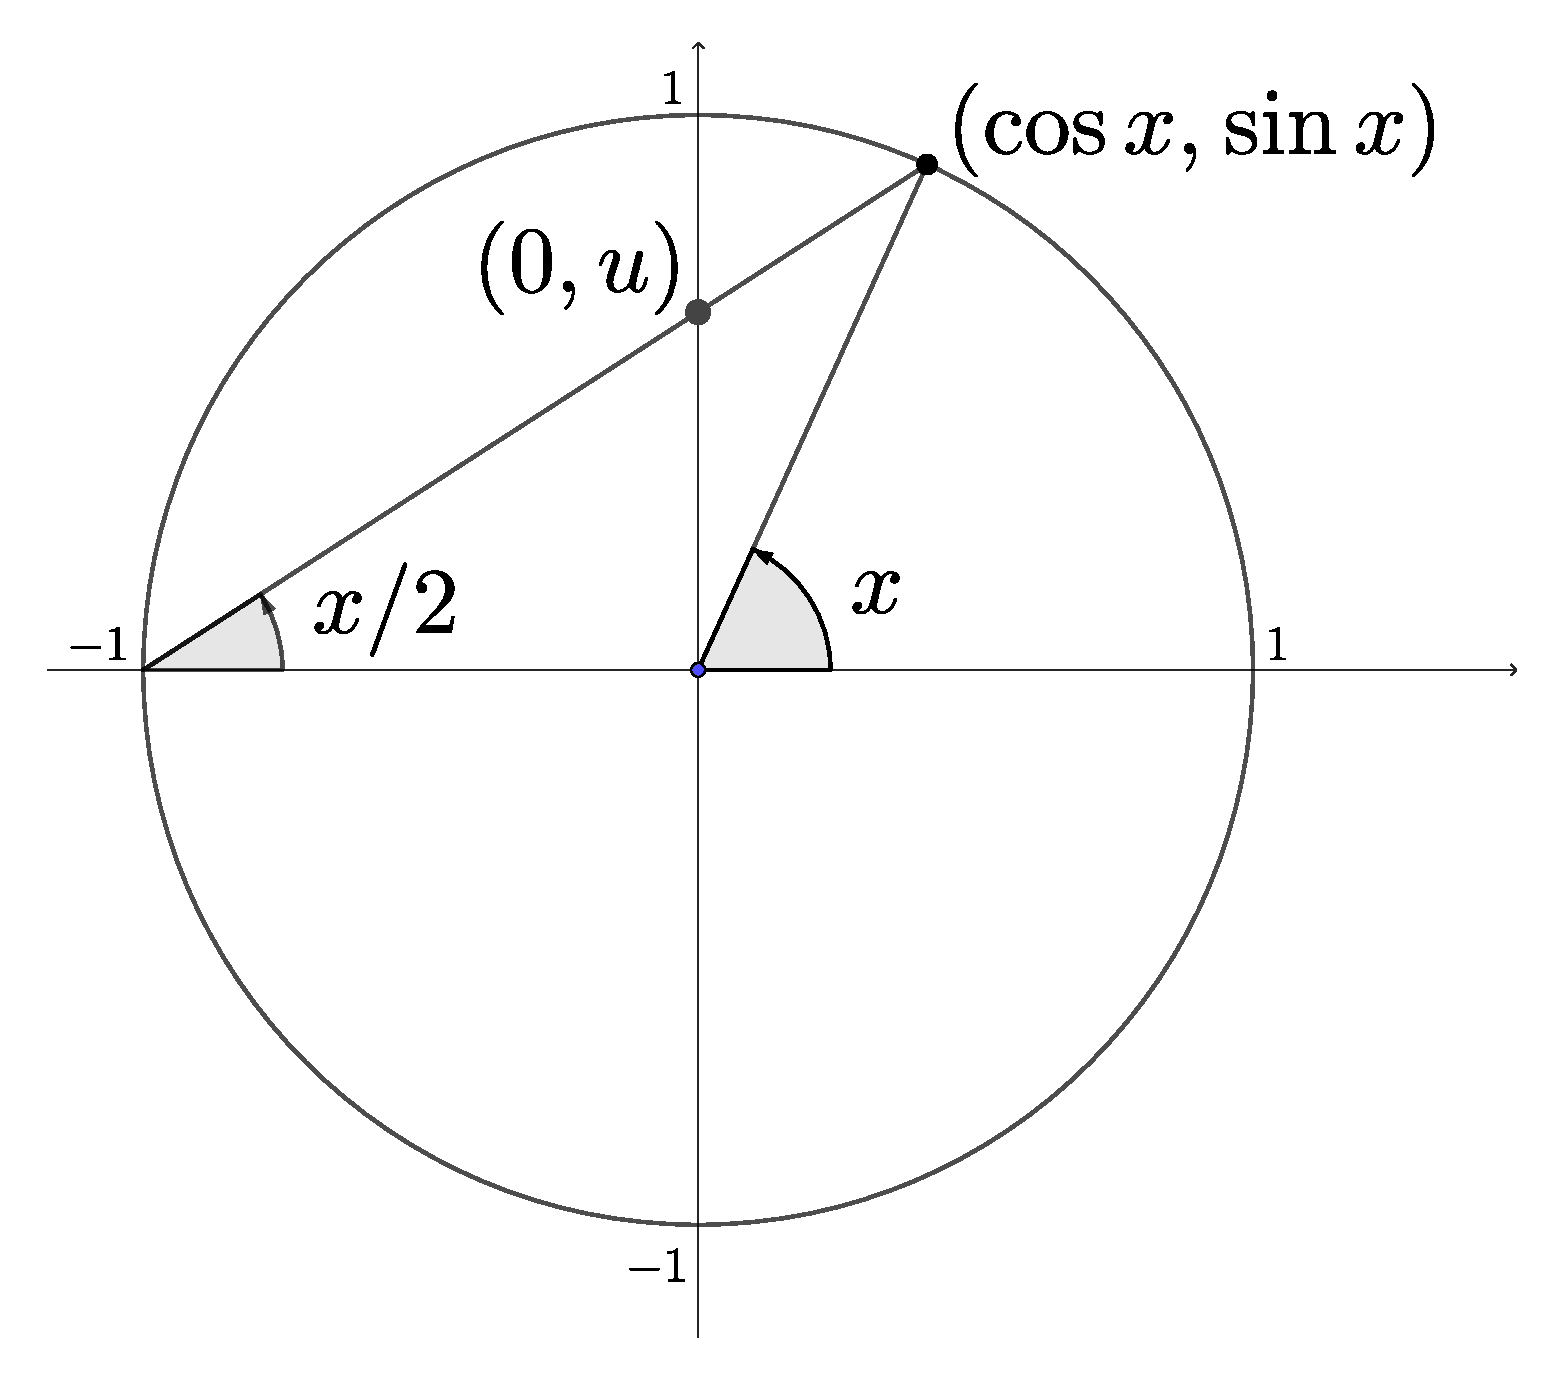
\includegraphics[height=7cm]{03/u-tanx2.pdf}
\end{figure}

\newpage

前ページで紹介した「$\cos x$ と $\sin x$ と定数の四則演算だけで構成される関数」の中でもさらに
\begin{center}
  $\cos^2 x$ と $\sin^2 x$ と $\left( \sin x \right) \left(\cos x\right)$ と定数の四則演算だけで構成される関数
\end{center}
に関しては,変数変換 $\ds u=\tan x$ による置換積分で計算することもできる.例として
\[
  \int_{0}^{\pi/4} \frac{1+\cos^2x}{\sin^2 x + 3 \cos^2 x} \ dx
\]
を計算してみよう.さっそく $\ds u=\tan x$ とおく.このとき,
\[
  \cos^2 x = \frac{1}{1+\tan^2 x} = \frac{1}{1+u^2} \qquad \sin^2 x = 1- \cos^2 x = 1- \frac{1}{1+u^2} = \frac{u^2}{1+u^2}
\]
である.ちなみに,今回は使わないが
\[
  \left( \sin x \right) \left(\cos x\right) = \frac{\sin x}{\cos x}~ \cos^2 x = \left( \tan x \right)\left( \cos^2 x\right)
  = \frac{u}{1+u^2}
\]
である.さらに,
\[
  \frac{du}{dx} = 1+\tan^2 x = 1+u^2 \quad \text{ より } \quad 1 = \frac{1}{1+u^2} \frac{du}{dx} 
\]
である.また,積分範囲は $
\begin{array}{c|ccc}
  x & 0 & \to & \pi/4\\ \hline
  u & 0 & \to & 1
\end{array}
$ と変換されるので,この積分は次のように計算できる.
\[
  \begin{aligned}
    \int_{0}^{\pi/4} \frac{1+\cos^2x}{\sin^2 x + 3 \cos^2 x} \ dx
    &= \int_{0}^{\pi/4} \frac{1+ \frac{1}{1+u^2}}{ \frac{u^2}{1+u^2} + \frac{3}{1+u^2}} \frac{1}{1+u^2}~ \frac{du}{dx} \ dx
      = \int_{0}^{1} \frac{u^2+2}{(u^2+1)(u^2+3)} \ du\\[2ex]
    &= \int_{0}^{1}\left(\frac{\frac{1}{2}}{u^2+1} + \frac{\frac{1}{2}}{u^2+3}\right) \ dx 
      = \frac{1}{2}\left( \Big[ \tan^{-1}u \Big]_{0}^{1} + \left[ \frac{1}{\sqrt{3}}
      \tan^{-1}\frac{u}{\sqrt{3}}\right]_{0}^{1}\right)\\[2ex]
    &=\frac{\pi}{8}  + \frac{\sqrt{3}~\pi}{36}
  \end{aligned}
\]

なお,この変数変換における $u$ と $x$ の関係には下図のような意味づけができる.
\begin{figure}[h]
  \centering
  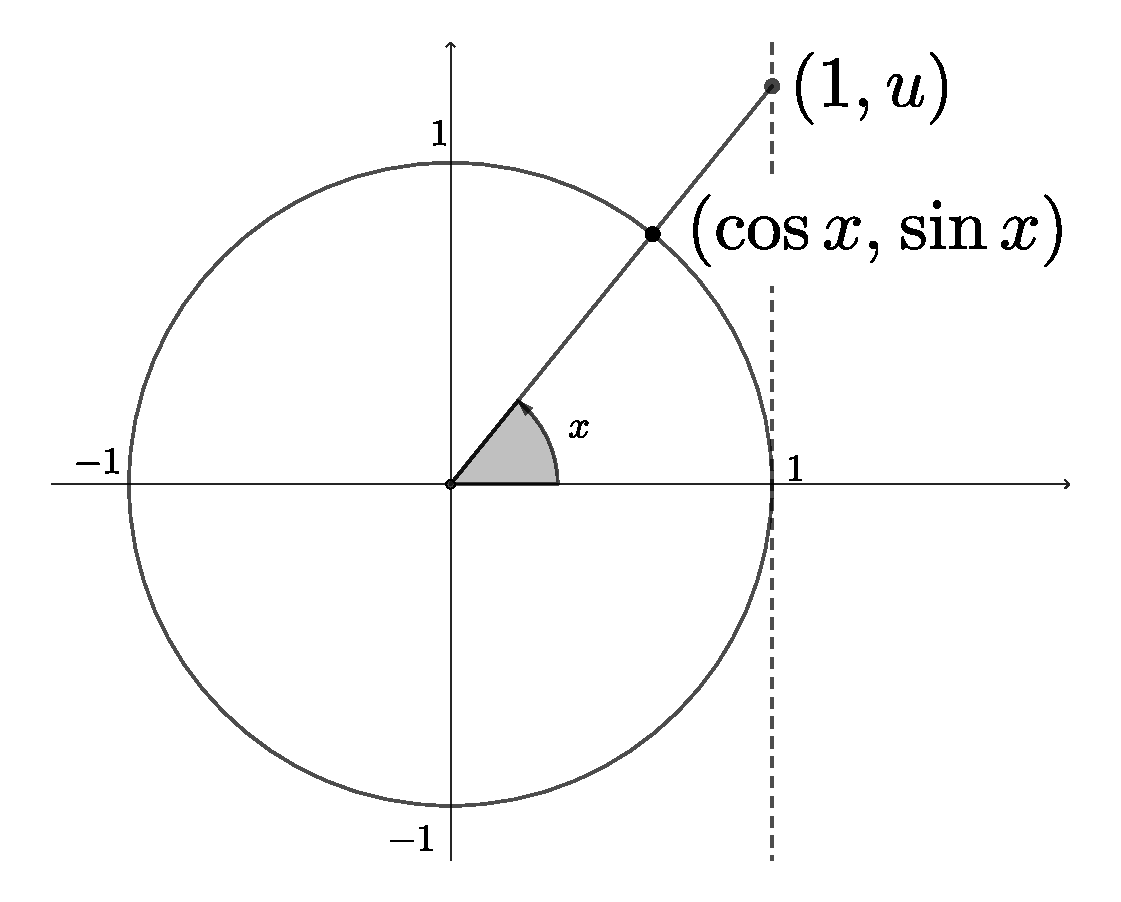
\includegraphics[height=6.5cm]{03/u-tanx.pdf}
\end{figure}

\newpage

さらに特別な場合として,$\left(\sin^m x\right)\left(\cos^nx\right)$ の
積分を考える.例として,以下の $m=2,n=3$ の場合を計算してみるが,$m,n$
の少なくとも一方が奇数なら同様に計算できる.
  \[
    \int_{0}^{\pi/2} \left( \sin^2 x\right) \left( \cos^3 x \right) \ dx
  \]
  これも $\ds u=\tan\frac{x}{2}$ による置換積分で分数関数の積分に帰着できるが,かなり面倒な計算になる.そこで
  \[
    \left( \sin^2 x\right) \left( \cos^3 x\right) = \left( \sin^2 x\right) \left(\cos^2 x\right) \cos x
    = \left( \sin^2 x\right)\left(1-\sin^2 x\right) \cos x
  \]
  と変形してみると,$u=\sin x$ による置換積分がうまくいきそうなことに気
  がつける.実際,$\ds \frac{du}{dx} = \cos x$ であり,積分範囲が
  \[
    \begin{array}{c|ccc}
      x & 0 & \to & \pi/2\\ \hline
      u & 0 & \to & 1
    \end{array}
  \]
  と変換されるので,以下のように割と簡単に計算できてしまう.
  \[
    \int_{0}^{\pi/2} \left( \sin^2 x\right) \left( \cos^3 x\right) \ dx
    = \int_{0}^{1} u^2 \left( 1-u^2\right) \ du = \left[ \frac{u^3}{3} - \frac{u^5}{5}\right]_{0}^{1} = \frac{2}{15}
  \]\\

  続いて,以下の $m=2,n=4$ の場合を計算してみる.$m,n$ の両方が偶数なら同様に計算できる.
  \[
    \int_{0}^{\pi/2} \left( \sin^2 x\right) \left( \cos^4 x\right) \ dx
  \]
  これも $\ds u=\tan\frac{x}{2}$ や $u=\tan x$ による置換積分で分数関数
  の積分に帰着はできるが,まず
  \[
    \left( \sin^2 x\right) \left( \cos^4 x\right) = \left( 1-\cos^2 x\right) \cos^4 x  = \cos^4x - \cos^6 x
  \]
  と変形してみる.ここで半角の公式から
  \[
    \begin{aligned}
      \cos^4 x &= \left( \cos^2 x\right)^2 =
      \left(\frac{1+\cos(2x)}{2}\right)^2 = \frac{1+2\cos(2x) +
        \cos^2(2x)}{4}
      = \frac{1+2\cos(2x) + \frac{1+\cos(4x)}{2}}{4}\\
      &= \frac{3}{8} + \frac{\cos (2x)}{2} + \frac{\cos (4x)}{8}\\ \\
      \cos^6 x &= \left( \cos^2 x\right)^3 = \left(
        \frac{1+\cos(2x)}{2}\right)^3 = \frac{1+3\cos(2x) +
        3\cos^2(2x) + \cos^3(2x)}{8}\\
      &= \frac{1+3\cos(2x) + 3 \frac{1+\cos(4x)}{2}}{8} + \frac{\cos^3(2x)}{8}
      = \frac{5}{16} + \frac{3}{8}\cos(2x) + \frac{3}{16}\cos(4x) + \frac{\cos^3(2x)}{8}
    \end{aligned}
  \]
  なので,この積分は以下のように計算できる.
  \[
    \begin{aligned}
      \int_{0}^{\pi/2} \left(\sin^2 x\right)\left(\cos^4x\right) \ dx
      &= \int_{0}^{\pi/2}\left( \frac{1}{16} + \frac{\cos(2x)}{8} - \frac{\cos(4x)}{16} - \frac{\cos^3(2x)}{8}\right) \ dx\\
      &= \left[\frac{x}{16} + \frac{\sin(2x)}{16} - \frac{\sin(4x)}{64}\right]_{0}^{\pi/2}
      - \frac{1}{8}\int_{0}^{\pi/2}\cos^3(2x) \ dx\\
      & = \frac{\pi}{32} - \frac{1}{8}\int_{0}^{\pi/2}\cos^3(2x) \ dx = \frac{\pi}{32}
    \end{aligned}
  \]
  最後に残った積分は,$\cos^3(2x) = \left(1-\sin^2(2x)\right)
  \cos(2x)$ と変形できるので $u=\sin(2x)$ による置換積分で計算できる.
 


\end{document}


\documentclass[10pt, uplatex, dvipdfmx]{jsarticle}
\usepackage{../mypackage}

\graphicspath{{../pictures}}

\setcounter{section}{3}

\begin{document}

\section{広義積分}\label{sec:imporper}

これまでの積分は有界閉区間上の有界な関数のみを対象にしてきた.その制
限を除き,(半)開区間や無限区間上の有界とは限らない関数の積分を定義
する.


\subsection{広義積分の定義}

\begin{definition}
  $f$ を半開区間 $[a,b) \; (b=\infty \text{でもよいが,その場合は半開
    区間とは呼ばないかも})$ で定義された1変数関数とし,任意
  の $c \in [a,b)$ 対し有界閉区間 $[a,c]$ で $f$ は有界で積分可能である
  とする.このとき,
  \[
    \int_{a}^{b} f(x) \ dx := \lim_{c \to b-0} \int_{a}^{c} f(x) \ dx
    \quad \left(b =\infty \text{ なら }\int_{a}^{\infty} f(x) \ dx := \lim_{c \to \infty}
      \int_{a}^{c} f(x) \ dx\right)
  \]
  を $f$ の半開区間 $[a,b)$ における\textbf{広義積分}という.極限が存在
  するとき広義積分は\textbf{収束する}といい,極限が存在しないとき
  は\textbf{発散する}という.

  同様にして,半開区間 $(a,b]\; (a=-\infty
  \text{でもよいが,半開区間とは呼ばないかも})$ における広義積分を
  \[
    \int_{a}^{b} f(x)\ dx := \lim_{c \to a+0} \int_{a}^{b} f(x) \ dx
    \quad \left( a = -\infty \text{ なら } \int_{-\infty}^{b} f(x) \
      dx := \lim_{c \to -\infty}  \int_{c}^{b} f(x) \
      dx\right)
  \]
  により定義する.このとき,$f$ は任意の $c \in (a,b]$ に対し有界閉区
  間 $[a,c]$ で有界で積分可能な関数とし,広義積分の収束・発散も同様に定
  義する.
  
  また,開区間 $(a,b) \; (a=-\infty \text{ や } b=\infty \text{でもよ
    い})$ で定義された関数 $f$ に対して,任意に $c \in (a,b)$ をとり
  \[
    \int_{a}^{b} f(x) \ dx := \int_{a}^{c} f(x)\ dx + \int_{c}^{b} f(x)\ dx
  \]
  により $f$ の開区間 $(a,c)$ における広義積分を定義する.このとき,右
  辺の2つの広義積分が共に収束するとき,左辺の広義積分は収束すると定義し,
  右辺のどちらか一方でも発散すれば左辺の広義積分も発散すると定義する.
  この広義積分が収束するとき,その値は $c$ によらない.

  関数が定義されない点が区間の内部に存在する場合は,区間をその点で分け
  て広義積分を定義する.例えば,関数 $f$ が$x=c \in (a,b)$ で定義されないなら
  \[
    \int_{a}^{b} f(x) \ dx := \int_{a}^{c} f(x) \ dx + \int_{c}^{b} f(x) \ dx
  \]
  により定義する.先程と同様に右辺の両方の広義積分が収束するときのみ左辺も収束すると定義する.
\end{definition}

\begin{example}
  \[
    \int_{0}^{\infty} e^{-x}\ dx = \lim_{c \to \infty} \int_{0}^{c} e^{-x}\ dx
    = \lim_{c \to \infty} \Big[-e^{-x}\Big]_{0}^{c} 
    = \lim_{c \to \infty} \left( -e^{-c} + 1\right) = 1
  \]
\end{example}

\begin{example}
  \[
    \int_{-\infty}^{0} e^{-x} \ dx = \lim_{c \to -\infty}
    \int_{c}^{0} e^{-x} \ dx = \lim_{c \to -\infty} \Big[ -e^{-x} \Big]_{c}^{0}
    = \lim_{c \to -\infty} \left( -1 + e^{-c}\right) = \infty \; \left( \text{ 発散 } \right)
  \]
\end{example}

\begin{example}
  \[
    \int_{0}^{1} \frac{dx}{\sqrt{1-x^2}} = \lim_{c \to 1-0}  \int_{0}^{c} \frac{dx}{\sqrt{1-x^2}}
    = \lim_{c \to 1-0} \Big[ \sin^{-1} x \Big]_{0}^{c} = \lim_{c \to 1-0} \sin^{-1}c 
    = \frac{\pi}{2}
  \]
\end{example}


\subsection{広義積分の収束・発散の判定}

広義積分の値はいつでもその値を計算できるとは限らないが,収束・発散の判
定だけならできることがある.

\begin{theorem}\label{thm:convergent}
  $f,g$ を区間 $[a, b)$ で $|f(x)| \leq g(x)$ を満たす1変数関数で,任意
  の $c \in [a,b)$ に対して $[a,c]$ で積分可能とする.このとき,広義積
  分 $\ds \int_{a}^{b} g(x)\ dx$ が収束するなら広義積分 $\ds \int_{a}^{b}
  f(x) \ dx$ も収束し,以下が成り立つ.
  \[
    \left| \int_{a}^{b} f(x)\ dx \right| \leq \int_{a}^{b} g(x)\ dx
  \]
\end{theorem}

\begin{theorem}\label{thm:divergent}
  $f,g$ を区間 $[a,b)$ で $f(x) \leq g(x)$ を満たす1変数関数で,任意
  の $c \in [a,b)$ に対して $[a,c]$ で積分可能とする.このとき,
  \[
    \int_{a}^{b} f(x) \ dx = +\infty \text{ ならば } \int_{a}^{b} g(x) \ dx = +\infty
  \]
  であり,
  \[
    \int_{a}^{b} g(x)\ dx = -\infty \text{ ならば } \int_{a}^{b} f(x)\ dx = -\infty
  \]
  である.
\end{theorem}

\begin{remark}
  定理\ref{thm:convergent}, \ref{thm:divergent}は区間が $(a,b], (a,b)$
  の場合(無限区間でもよい)に対しても成り立つ.
\end{remark}


\begin{example}
  広義積分 $\ds \int_{0}^{\infty} \frac{\sin x}{(x+1)(x+2)}\ dx$ は収束する.
  
  \begin{proof}
    区間 $[0, \infty)$ において
    \[
      \left|\frac{\sin x}{(x+1)(x+2)}\right| \leq \frac{1}{(x+1)^2}
    \]
    であり,任意の $c \in [0, \infty)$ に対して
    $\ds \frac{\sin x}{(x+1)(x+2)}, \, \frac{1}{(x+1)^2}$ は $[0,c]$ で
    連続なので積分可能である.さらに,
    \[
      \int_{0}^{\infty} \frac{dx}{(x+1)^2} = \lim_{b \to \infty} \int_{0}^{b} \frac{dx}{(x+1)^2}
      = \lim_{b \to \infty} \left[ -\frac{1}{x+1}\right]_{0}^{b}
      =\lim_{b \to \infty}\left( -\frac{1}{b+1} +1\right) =1
    \]
    より,定理\ref{thm:convergent}から広義積分
    $\ds \int_{0}^{\infty}\frac{\sin x}{(x+1)(x+2)}\ dx$ は収束する.
  \end{proof}
\end{example}

\begin{example}
  広義積分 $\ds \int_{1}^{\infty} \frac{dx}{1+\log x}$ は $+\infty$ に発散する.

  \begin{proof}
    区間 $[1,\infty)$ において
    \[
      \frac{1}{1+x} < \frac{1}{1+\log x}
    \]
    であり,任意の $c \in [1, \infty)$ に対して
    $\ds \frac{1}{1+x}, \, \frac{1}{1+\log x}$ は $[1, c]$ で連続なので積分可能であ
    る.さらに,
    \[
      \int_{1}^{\infty} \frac{dx}{1+x} = \lim_{b \to \infty} \int_{1}^{b} \frac{dx}{1+x}
      =\lim_{b \to \infty} \left[ \log (1+x) \right]_{1}^{b}
      = \lim_{b \to \infty} \left( \log(1+b) - \log 2\right) = +\infty
    \]
    より,定理\ref{thm:divergent}から広義積分
    $\ds \int_{1}^{\infty} \frac{dx}{1+\log x}$ は $+\infty$ に発散す
    る.
  \end{proof}
\end{example}

\begin{example}
  広義積分 $\ds \int_{0}^{3} \frac{\log x}{x} \ dx$ は $-\infty$ に発散する.

  \begin{proof}
    区間  $(0,3]$ において
    \[
      \frac{\log x}{x} \leq \frac{x-1}{x}
    \]
    であり,任意の $c \in (0,3]$ に対して
    $\ds \frac{\log x}{x}, \, \frac{x-1}{x}$ は $[c,3]$ で連続なので積
    分可能である.さらに,
    \begin{align*}
      \int_{0}^{3}\frac{x-1}{x} \ dx &= \lim_{a \to +0} \int_{a}^{3} \frac{x-1}{x}\ dx
                                       = \lim_{a \to +0}\int_{a}^{3} \left( 1-\frac{1}{x}\right)\ dx
                                       = \lim_{a \to +0}\left[ x-\log x\right]_{a}^{3} \\
                                     &= \lim_{a \to +0}\left( 3-\log 3 -a + \log a\right)
                                       =-\infty
    \end{align*}
    より,定理\ref{thm:divergent}から広義積分
    $\ds \int_{0}^{3} \frac{\log x}{x}\ dx$ は $-\infty$ に発散する.
  \end{proof}
\end{example}

\subsection{積分と広義積分}

例えば,以下の積分の計算過程には広義積分が現れている.($1 = x'$ とみなして部分積分)
\[
  \int_{0}^{1} \sin^{-1} x \ dx = \Big[ x \sin^{-1} x \Big]_{0}^{1} - \int_{0}^{1} \frac{x}{\sqrt{1-x^2}} \ dx
  = \frac{\pi}{2} - \Big[ - \sqrt{1-x^2} \Big]_{0}^{1} = \frac{\pi}{2} - 1
\]
普通の積分計算に見えるかもしれないが,実は
$\ds \int_{0}^{1}\frac{x}{\sqrt{1-x^2}} \ dx$ が広義積分である.
\[
  \int_{0}^{1} \frac{x}{\sqrt{1-x^2}} \ dx = \lim_{c \to 1-0} \int_{0}^{c} \frac{x}{\sqrt{1-x^2}} \ dx
  = \lim_{c \to 1-0} \Big[-\sqrt{1-x^2}\Big]_{0}^{c} = \lim_{c \to 1-0} \left(1- \sqrt{1-c^2} \right) =1
\]
このように,実は広義積分だがそれに気づかずに計算してしまっても結果は正
しく得られているが,そうなるように広義積分がうまく定義されている.よかったね.\\

一方で,例えば以下の左辺はただの積分に見えるかもしれないが,被積分関数が $x=0$ で定義されていな
いので広義積分である.

\[
  \int_{-1}^{1} \frac{dx}{x} : = \int_{-1}^{0} \frac{dx}{x} + \int_{0}^{1} \frac{dx}{x}
\]
右辺のどちらの広義積分も発散するので,この左辺は発散すると広義積分では定義している.これに気づかず
\[
  \textbf{(間違い)} \quad \int_{-1}^{1} \frac{dx}{x} = \Big[ \log|x| \Big]_{-1}^{1} = \log 1 - \log 1 =0 \quad
  \textbf{(間違い)}
\]
と計算してしまうと,広義積分の定義とは合わない結論にたどり着いてしまう.気をつけよう.

\newpage

\subsection{練習問題}

次の広義積分の収束・発散を明らかにしよう.

\vspace{1zh}

\begin{edaenumerate}<3>[(1)]

  
\item $\ds \int_{0}^{1} \frac{dx}{\sqrt{x}}$
  
\item $\ds \int_{0}^{1} \frac{dx}{x}$

\item $\ds \int_{0}^{1} \frac{dx}{x^2}$

\item $\ds \int_{1}^{\infty} \frac{dx}{\sqrt{x}}$

\item $\ds \int_{1}^{\infty} \frac{dx}{x}$

\item $\ds \int_{1}^{\infty} \frac{dx}{x^2}$

\item $\ds \int_{-\infty}^{\infty} \frac{dx}{1+x^2}$

\item $\ds \int_{-\infty}^{\infty} \frac{dx}{x^2}$

\item $\ds \int_{-1}^{1} \frac{x}{\sqrt{1-x^2}}\ dx$

\item $\ds \int_{-\infty}^{\infty} x \ dx$

\item $\ds \int_{-\frac{\pi}{2}}^{\frac{\pi}{2}}\tan x\ dx$

\item $\ds \int_{0}^{1} x \log x\ dx$

\item $\ds \int_{0}^{1} \sqrt{1+\frac{1}{x^4}}\ dx$

\item $\ds \int_{0}^{\infty} x e^{-x^2}\ dx$

\item $\ds \int_{0}^{\infty} e^{-x^2}\ dx$

\end{edaenumerate}

\vspace{2zh}

「積分基本問題集 壱」$(36) \sim (48)$ も参考にしてください.

\begin{figure}[b]
  答え : (1), (6), (7), (9), (12), (14), (15) は収束.残りは発散.
\end{figure}

\newpage

\subsection{(おまけ)Beta 関数と Gamma 関数}

広義積分によって定義される関数として有名な Beta 関数と Gamma 関数を紹介
する.
\begin{theorem}[\textbf{Beta 関数}]
  以下の $2$ 変数関数 $B(p,q)$ は $p>0, q>0$ で定義され,\textbf{Beta 関
    数}と呼ばれる.
  \[
    B(p,q) := \int_{0}^{1} x^{p-1} (1-x)^{q-1} \ dx
  \]
\end{theorem}

\begin{proof}
  $p \geqq 1$ かつ $q \geqq 1$ ではこれはただの連続関数の積分なので,ちゃ
  んと値が定まる.問題は$0<p<1$ や $0<q<1$ で$B(p,q)$ が広義積分となる
  ので,それがちゃんと収束することを証明しておく.

  被積分関数を $\ds f(x) = x^{p-1}(1-x)^{q-1}$ として,次の $3$ つの場
  合に分けて示していく.
  \begin{enumerate}[(i)]

  \item $p \geqq 1$ かつ $0 < q < 1$ のとき:$a:=p-1, b:=1-q$ とおけ
    ば,$a \geqq 0$ かつ $0 < b < 1$ であり,
    \[
      f(x) = \frac{x^a}{(1-x)^b}
    \]
    と書ける.従って,$B(p,q)$ は半開区間 $[0,1)$ 上の広義積分であ
    る.$x \in [0,1)$ において
    \[
      |f(x)| = \left|\frac{x^a}{(1-x)^b}\right| \leqq \frac{1}{(1-x)^b}
    \]
    であり,最右辺の $[0,1)$ 上の広義積分が次のように収束する
    ので,定理\ref{thm:convergent}から $B(p,q)$ は収束する.
    \[
      \int_{0}^{1} \frac{dx}{(1-x)^b} = \lim_{c \to 1-0} \int_{0}^{c} (1-x)^{-b} \ dx
      = \lim_{c \to 1-0} \left[ \frac{(1-x)^{1-b}}{b-1}\right]_{0}^{c}
      =\lim_{c \to 1-0} \frac{ (1-c)^{1-b} - 1}{b-1} = \frac{1}{1-b}
    \]
    
  \item $0 < p < 1$ かつ $q \geqq 1$ のとき:$u=1-x$ とおいて置換積分を
    適用すれば,
    \[
      B(p,q) = \int_{0}^{1}  u^{q-1} (1-u)^{p-1} \ du \; \Big( = B(q,p) \Big)
    \]
    と書き換えられる.これが収束することは (i) で示した.
    
  \item $0 < p < 1$ かつ $0 < q < 1$ のとき:$a:=1-p, b:=1-q$ とおけ
    ば,$0<a<1$ かつ $0<b<1$ であり,
    \[
      f(x) = \frac{1}{x^a (1-x)^b}
    \]
    と書けるので,$B(p,q)$ は開区間 $(0,1)$ 上の広義積分である.従っ
    て,$B(p,q)$ を
    \begin{equation}\label{eq:divide_beta}
      B(p,q) = \int_{0}^{1/2} \frac{dx}{x^a(1-x)^b} + \int_{1/2}^{1} \frac{dx}{x^a (1-x)^b}
    \end{equation}
    と2個の広義積分の和に分けて両方が収束すること
    を示せばよい.第1項に関しては,$\ds x \in \left( 0, 1/2\right]$ に対して $1/2 \leqq 1-x < 1$ なので
    \[
      |f(x)| = \left| \frac{1}{x^a(1-x)^b} \right| \leqq \frac{2^b}{x^a}
    \]
    であり,この最右辺の半開区間 $(0, 1/2]$ 上の広義積分が以下のように収束する.
    \[
      \int_{0}^{1/2} \frac{2^b}{x^a} \ dx = \lim_{ c \to +0} 2^b
      \int_{c}^{1/2} x^{-a} \ dx = 2^b \lim_{ c \to +0}
      \left[\frac{x^{1-a}}{1-a}\right]_{c}^{1/2} = 2^b
      \lim_{c \to +0} \frac{2^{a-1} - c^{1-a}}{1-a} = \frac{2^{a+b-1}}{1-a}
    \]
    よって,定理\ref{thm:convergent}から(\ref{eq:divide_beta})の第1項は
    収束する.第2項は(ii)と同じ置換積分で第1項と同じ形に帰着でき
    る.\qedhere
  \end{enumerate}
\end{proof}

\begin{theorem}[\textbf{Gamma 関数}]
  以下の関数 $\varGamma(s)$ は $s>0$ で定義され,\textbf{Gamma 関数} と呼ばれる.
  \[
    \varGamma(s) := \int_{0}^{\infty} e^{-x} x^{s-1} \ dx
  \]
\end{theorem}

\begin{proof}
  広義積分 $\varGamma(s)$ を以下のように $x=1$ で2個に分ける.
  \begin{equation}\label{eq:divide_gamma}
    \varGamma(s) = \int_{0}^{1} e^{-x} x ^{s-1}  \ dx  + \int_{1}^{\infty} e^{-x} x^{s-1} \ dx
  \end{equation}
  
  まず,右辺第1項を考える.$s \geqq 1$ ではこれはただの有界閉区間上の連
  続関数の積分なので,ちゃんと値が定まる.$0<s<1$ ではこれは半開区間 $(0,
  1]$ 上の広義積分である.このとき,$x \in (0, 1]$ に対して
  \[
    \left| e^{-x} x^{s-1}\right|  \leqq x^{s-1}
  \]
  であり,この右辺の半開区間 $(0, 1]$ 上の広義積分は以下のように収束す
  るから,定理\ref{thm:convergent}により(\ref{eq:divide_gamma})の右辺第1項
  は収束する.
  \[
    \int_{0}^{1} x^{s-1} \ dx = \lim_{c \to +0} \int_{c}^{1} x^{s-1} \
    dx = \lim_{c \to +0} \left[ \frac{x^{s}}{s}\right]_{c}^{1}
    = \lim_{c \to +0} \frac{1-c^s}{s} = \frac{1}{s}
  \]

  次に,(\ref{eq:divide_gamma})の第2項の広義積分が収束することを示す.$s >0$ とする.$s+1>1$ なので
  \[
    \lim_{x \to \infty} e^{-x} x^{s+1} = 0
  \]
  だから,十分大きな $x$ に対して $e^{-x} x^{s+1} <1 $ である.そこ
  で,$x \geqq X$ では $e^{-x} x^{s+1} <1$ であるとすれば (\ref{eq:divide_gamma})の右辺第2項は
  \begin{equation}\label{eq:divide-X}
    \int_{1}^{\infty} e^{-x}x^{s-1} \ dx = \int_{1}^{X} e^{-x}x^{s-1} \ dx + \int_{X}^{\infty} e^{-x} x^{s-1} \ dx
  \end{equation}
  と分けられ,この右辺第1項はただの連続関数の積分なので,右辺第2項が収
  束することを示せばよい.このとき,$x \in [X, \infty)$ に対して
  \[
    \left| e^{-x} x^{s-1}\right| = \frac{e^{-x}x^{s+1}}{x^2} < \frac{1}{x^2}
  \]
  であり,この最右辺の無限区間 $[X, \infty)$ 上の広義積分は以下のように収束する.
  \[
    \int_{X}^{\infty} \frac{dx}{x^2} = \lim_{c \to \infty} \int_{X}^{c} x^{-2} \ dx = \lim_{ c \to \infty} \Big[-x^{-1} \Big]_{X}^{c}
    = \lim_{c \to \infty} \left( \frac{1}{X} - \frac{1}{c}\right) = \frac{1}{X}
  \]
  よって,定理\ref{thm:convergent}より(\ref{eq:divide-X}) の右辺第2項の広義積分は収束する.
\end{proof}

\begin{remark}
  Gamma 関数 $\varGamma(s)$ は自然数の階乗 $n! = n (n-1)\cdots 2 \cdot 1$ の拡張と見なせる.実際,部分積分により
  \[
    \varGamma(s+1) = \int_{0}^{\infty} e^{-x} x^{s} \ dx = \Big[e^{-x}x^{s}\Big]_{0}^{\infty} + s \int_{0}^{\infty} e^{-x} x^{s-1} \ dx
    = \lim_{c \to \infty} e^{-c}c^s + s \varGamma(s) = s\varGamma(s)
  \]
  となるので,自然数 $n$ に対しては
  \[
    \begin{aligned}
      \varGamma(n) &= (n-1) \varGamma(n-1) = (n-1)(n-2) \varGamma(n-2) = \cdots = (n-1)(n-2) \cdots 2 \cdot 1 \cdot \varGamma(1)\\
                   & = (n-1)! \varGamma(1) = (n-1)! \int_{0}^{-\infty} e^{-x} \ dx  = (n-1)! \lim_{c \to \infty} \Big[-e^{-x}\Big]_{0}^{c}
                     = (n-1)!
    \end{aligned}
  \]
  である.番号が1つずれるのが少し気持ち悪いが,とにかく $\Gamma(n) = (n-1)!$ となっている.
\end{remark}



\end{document}


\addtocontents{toc}{\newpage}

\documentclass[10pt, uplatex, dvipdfmx]{jsarticle}
\usepackage{../mypackage}

\graphicspath{{../pictures}}

\setcounter{section}{4}

\begin{document}

\section{平面図形の面積と曲線の長さ}\label{sec:area}


\subsection{平面図形の面積と積分}

\begin{theorem}\label{thm:area}
  $f,g$ を有界閉区間 $[a,b]$ 上の連続関数とし,$[a,b]$ で $f(x) \geqq
  g(x)$ とする.図\ref{fig:area}のように曲
  線 $y=f(x)$ と$y=g(x)$ と $x$ 軸に垂直な $2$ 直線 $x=a, \, x=b$ で囲
  まれる有界閉領域
  \[
    D=\Set{(x,y) | a \leqq x \leqq b, \, g(x) \leqq y \leqq f(x)}
  \]
  の面積は以下の積分値に等しい.
  \[
    \int_{a}^{b} \left( f(x) - g(x) \right) dx
  \]
  \begin{figure}[h]
    \centering
    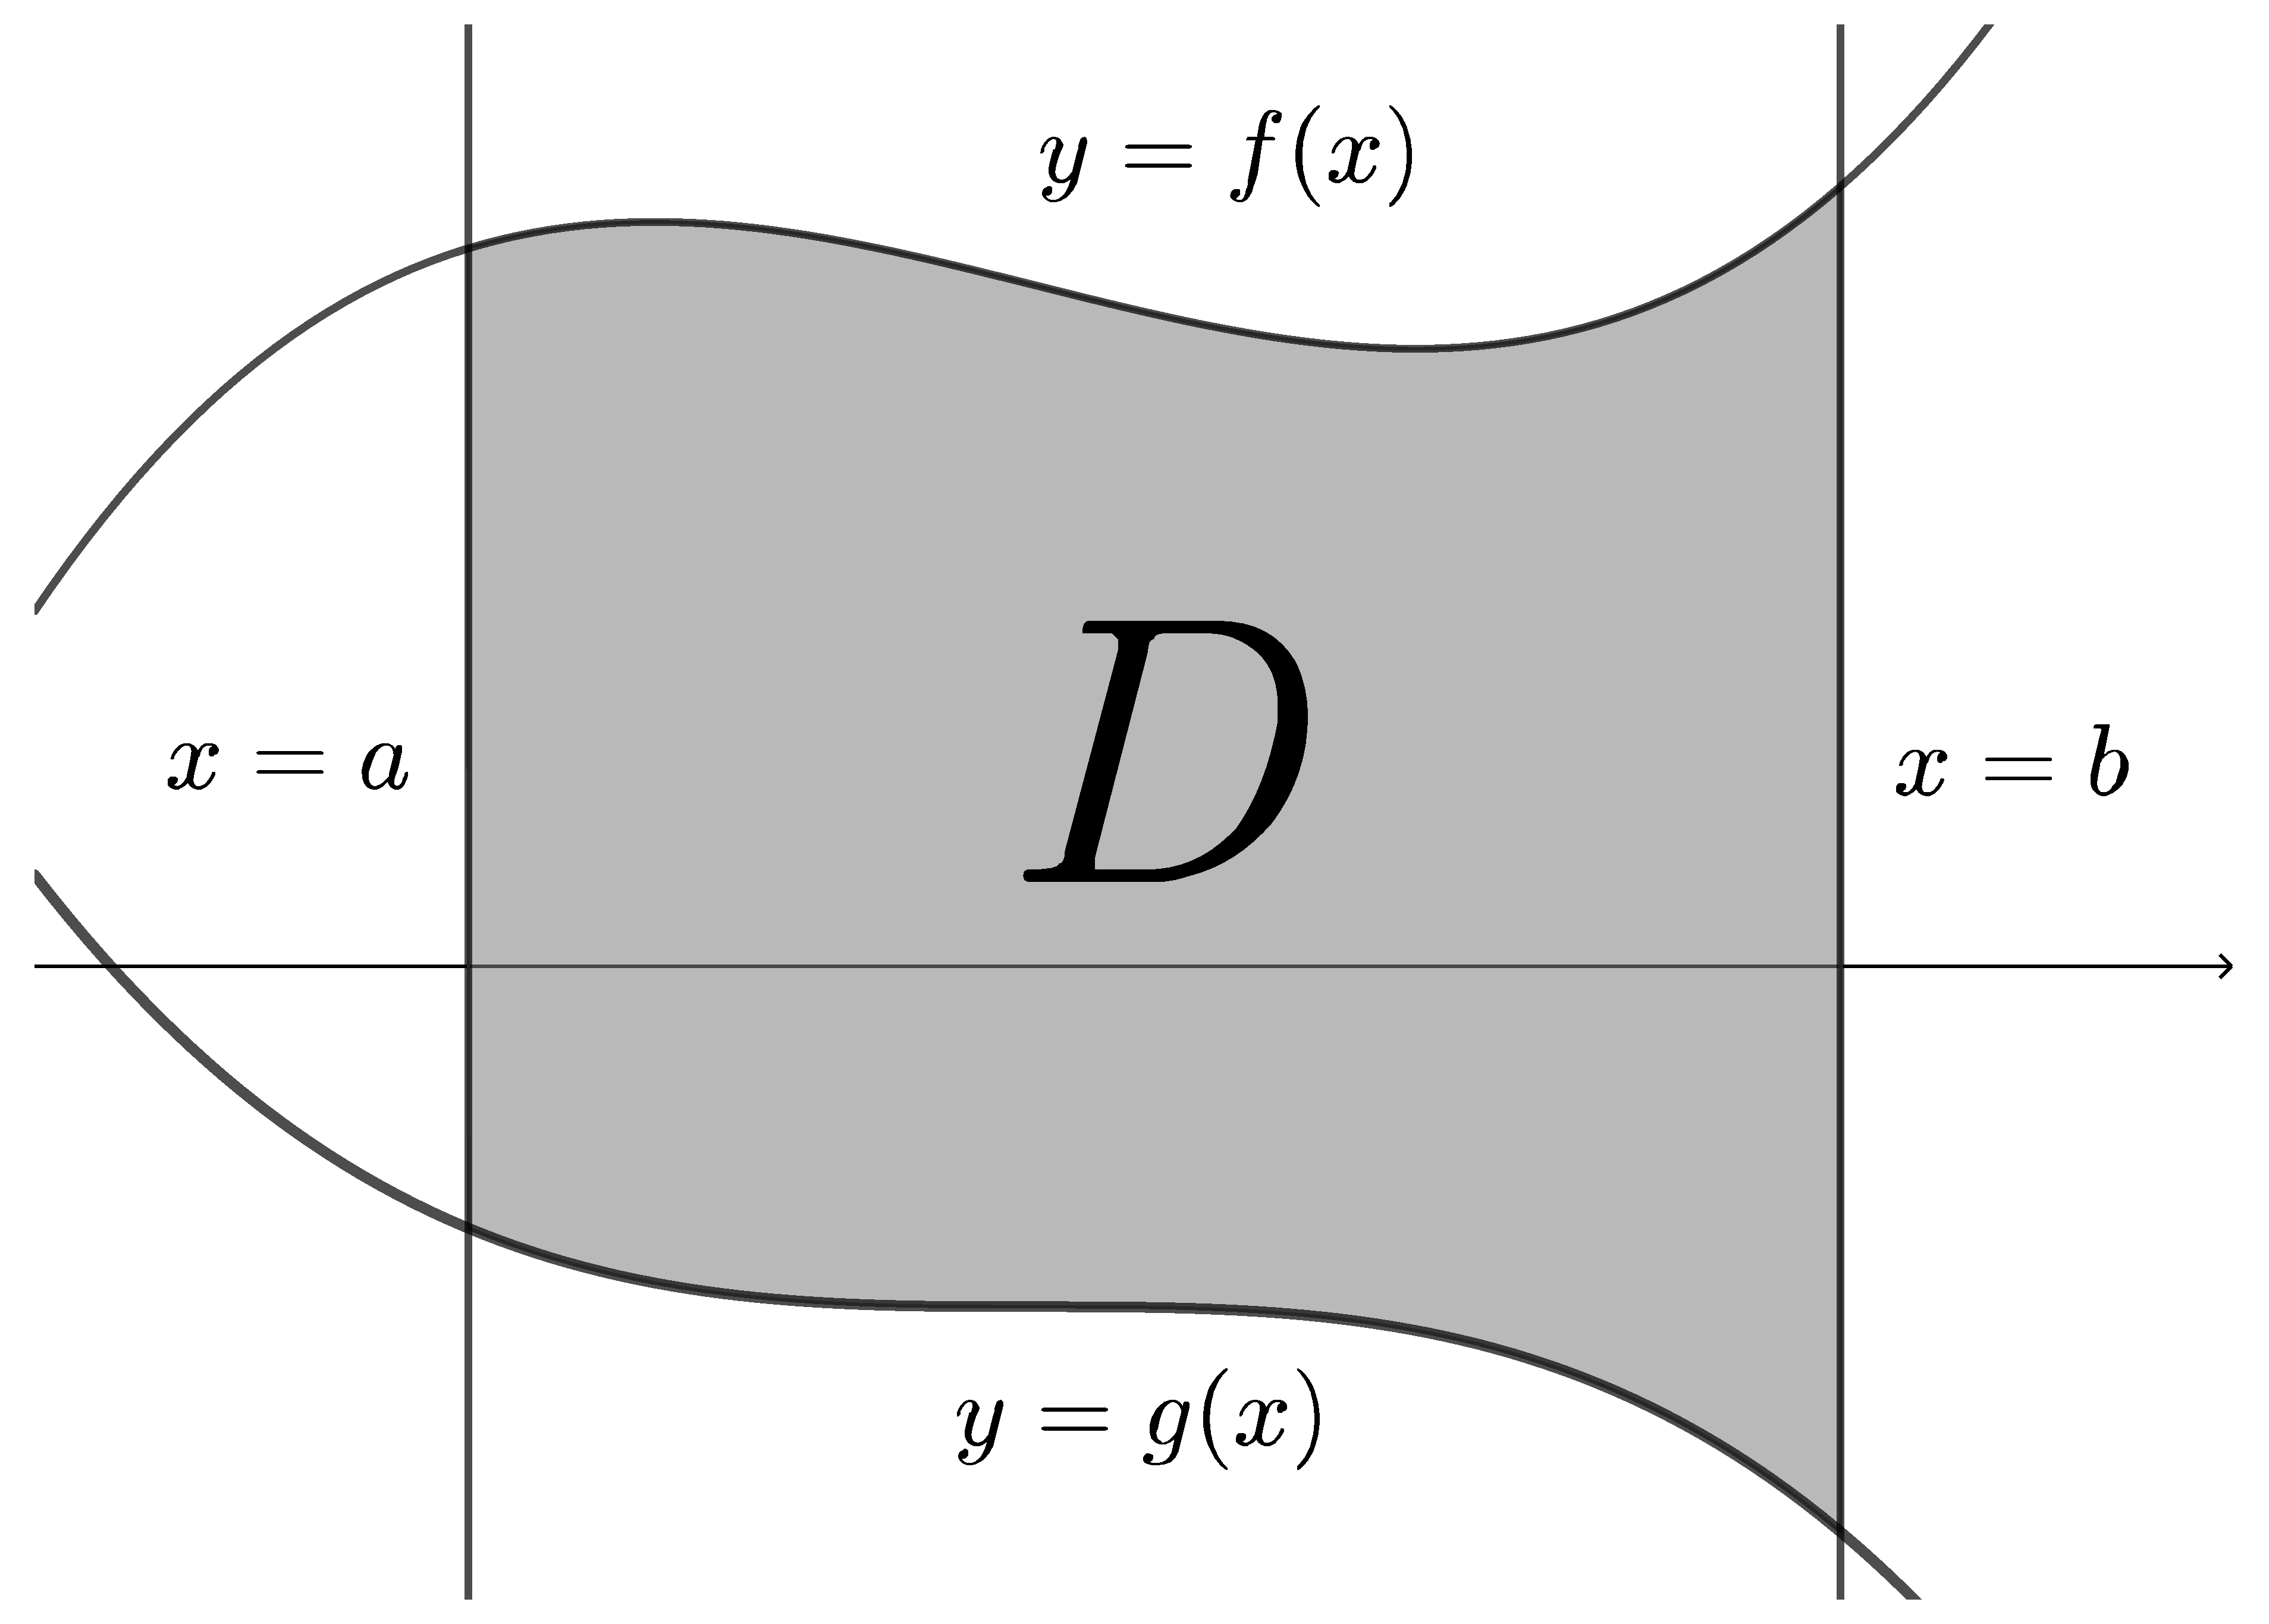
\includegraphics[width=7cm]{05/area.pdf}
    \caption{曲線 $y=f(x)$ と $y=g(x)$ と直線 $x=a$ と $x=b$ で囲まれる有界閉領域 $D$}
    \label{fig:area}
  \end{figure}
\end{theorem}


\begin{example}
  半径 $R>0$ の円の面積 $S(R)$ は図\ref{fig:circle}のように以下の積分で求められる.
  \[
    S(R) =\int_{-R}^{R} \left( \sqrt{R^2-x^2} - \left(-\sqrt{R^2-x^2}\right) \right) dx = \pi R^2
  \]
  \begin{figure}[h]
    \centering
    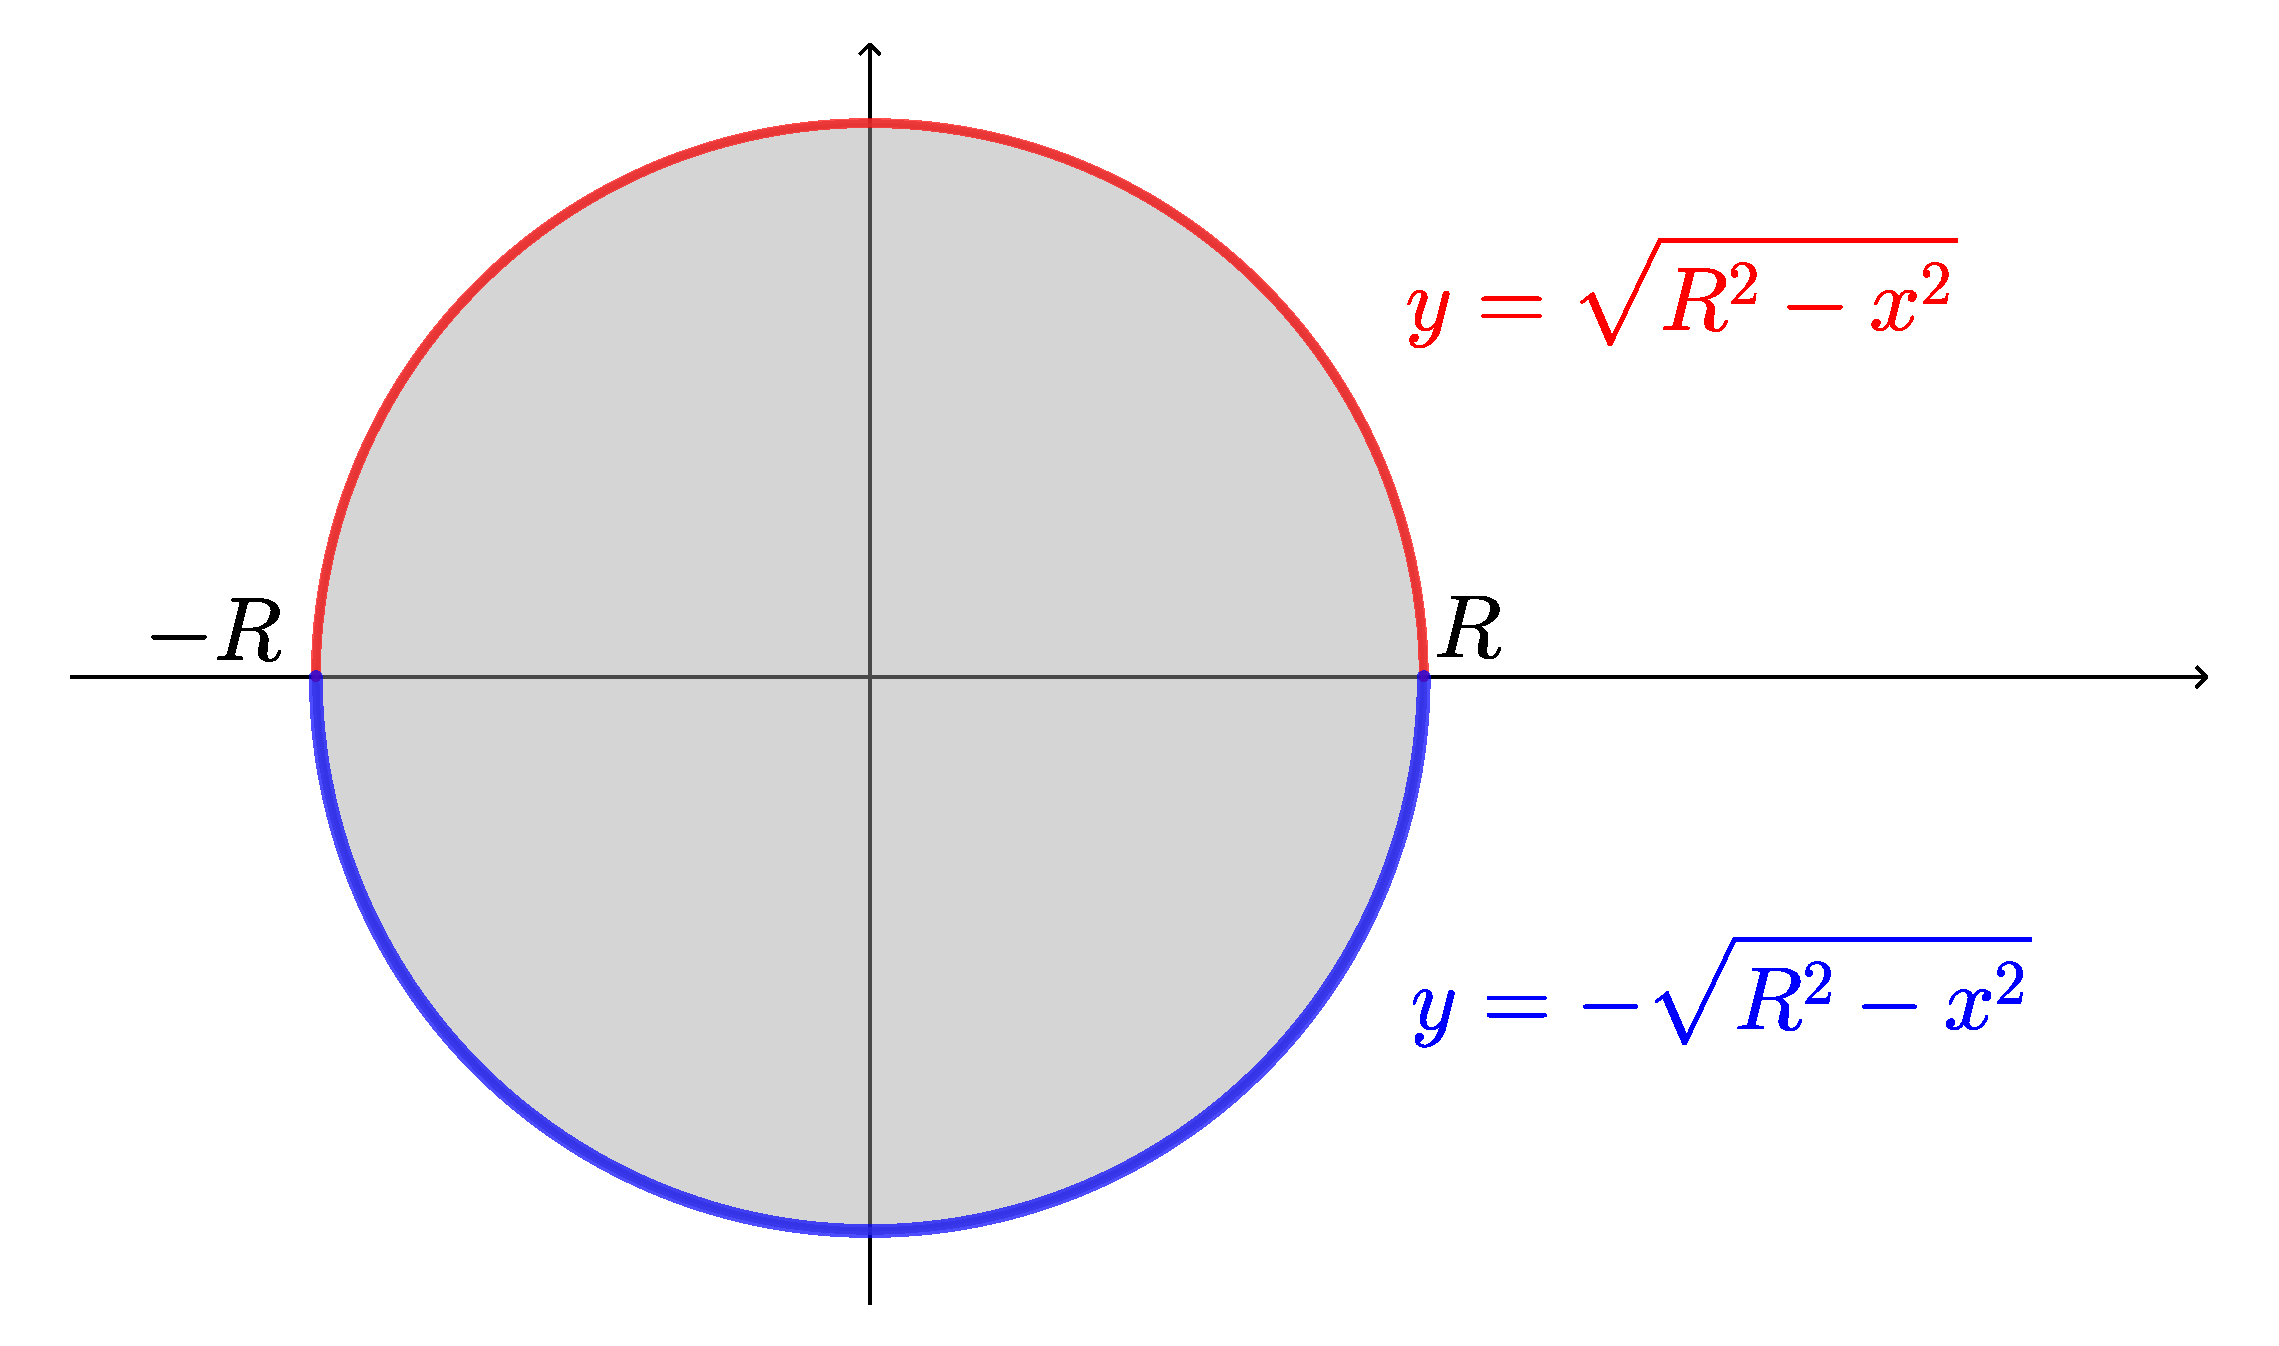
\includegraphics[width=8cm]{05/circle.pdf}
    \caption{曲線 $y=\pm \sqrt{R^2-x^2}$ と直
      線 $x= \pm R$ で囲まれる有界閉領域}
    \label{fig:circle}
  \end{figure}
\end{example}



\subsection{平面曲線の長さと積分}

積分を用いて曲線の長さを計算する.その前に「曲線の長さ」とは何かを定義
する.

$\varphi(t), \psi(t)$ を有界閉区間 $[a,b]$ 上定義された $C^1$ 級関数と
する.変数 $t$ が $a$ から $b$ まで動くとき,平面上の点
$\left( \varphi(t), \psi(t)\right)$ はなめらかな平面曲線 $C$ を描く.こ
れを
\[
  x=\varphi(t), \quad y=\psi(t), \quad a \leqq t \leqq b
\]
と書き,曲線 $C$
の\textbf{媒介変数表示}という.$\left( \varphi(a), \psi(a)\right), \,
\left(\varphi(b), \psi(b)\right)$ は $C$ の端点である.

曲線 $C$ を折れ線で近似する.閉区間 $[a,b]$ の分割
\[
  \Delta : a =t_0 < t_1 < t_2 < t_3< \cdots < t_{n-1} < t_n = b
\]
をとる.これにより曲線 $C$ 上に $n+1$ 個の点
$P_i\left( \varphi(t_i), \psi(t_i)\right) (i=0,1,\ldots, n)$ がとれる.
点 $P_0$ から $P_n$ までを順に結んで図\ref{fig:curve}のように曲線 $C$
を近似する折れ線ができる.
\begin{figure}[h]
  \centering
  \includegraphics[height=8cm]{05/curve.pdf}
  \caption{曲線 $C : x=\varphi(t), y=\psi(t)$ を近似する折れ線}
  \label{fig:curve}
\end{figure}

ここで
\[
\Delta x_i=\varphi(t_i)-\varphi(t_{i-1}), \quad \Delta y_i =\psi(t_i) - \psi(t_{i-1}), \quad
\Delta t_i = t_{i}-t_{i-1}
\]
とすれば,各線分 $P_{i-1}P_i$ の長さは三平方の定理から $\sqrt{{\Delta x_i}^2 + {\Delta
    y_i}^2}$ なので,$C$ を近似する折れ線の長さ $l_{\Delta}$ は次のように書ける.
\[
  l_{\Delta} = \sum_{i=1}^{n}\sqrt{{\Delta x_i}^2 + {\Delta y_i}^2} 
\]
そこで,$|\Delta| \to 0$ のときの $l_{\Delta}$ の極限値を曲線 $C$ の長
さと定義する.

次に,曲線 $C$ の長さ $\ds \lim_{|\Delta| \to 0} l_{\Delta}$ を積分を用
いて表す.まず,$l_{\Delta}$ は
\[
  \sqrt{{\Delta x_i}^2 + {\Delta y_i}^2} 
  =\sqrt{ \left(\frac{\Delta x_i}{\Delta
        t_i}\right)^2 + \left( \frac{\Delta y_i}{\Delta t_i}\right)^2
  }\ \Delta t_i
\]
と書ける.ここで,$\varphi, \psi$ は $C^1$ 級なので平均値の定理から
各 $i=1,2,\ldots, n$ に対して
\begin{align*}
  \frac{\Delta x_i}{\Delta t_i} = \frac{\varphi(t_i) - \varphi(t_{i-1})}{t_{i}-t_{i-1}} = \varphi'(c_i), \quad
  \frac{\Delta y_i}{\Delta t_i} = \frac{\psi(t_i) - \psi(t_{i-1})}{t_{i}-t_{i-1}} = \psi'(d_i)
\end{align*}
を満たす $c_i, d_i \in [t_{i-1}, t_{i}]$ が存在する.ここ
で,$\psi$ は $C^1$ 級と仮定したから $\psi'$ は連続である.よっ
て,$|\Delta| \to 0$のとき $d_i \to c_i$ なので $\psi'(d_i) \to
\psi'(c_i)$ である.従って,
\begin{align*}
  \lim_{|\Delta| \to 0} l_{\Delta} 
  = \lim_{|\Delta| \to 0} \sum_{i=1}^{n} \sqrt{ {\varphi'(c_i)}^2 + {\psi'(c_i)}^2}\ \Delta t_i
\end{align*}
である.これは分割 $\Delta$ と代表点集合 $\Set{c_i}$ に関する連続関
数 $\ds \sqrt{ {\varphi'(t)}^2 +
  {\psi'(t)}^2}$ の Riemann 和の $|\Delta| \to 0$ のときの極限なので,その値は
\[
  \int_{a}^{b} \sqrt{{\varphi'(t)}^2 + {\psi'(t)}^2} \ dt
\]
に等しい.以上を定理としてまとめておこう.

\begin{theorem}\label{thm:lencurve}
  $\varphi, \psi$ を閉区間 $[a,b]$ 上定義された $C^1$ 級関数とする.媒介変数表示
  \[
     x=\varphi(t), \; y=\psi(t), \; a \leqq t \leqq b
  \]
  で与えられる曲線の長さは,以下の積分値に等しい.
  \[
    \int_{a}^{b} \sqrt{ {\varphi'(t)}^2 + {\psi'(t)}^2} \ dt
  \]
\end{theorem}

\ \\

平面曲線の中でも,1変数関数 $y=f(x) \; (a \leqq x \leqq b)$ のグラフと
して与えられる曲線は
\[
  x = t, \; y= f(t), a \leqq t \leqq b
\]
と媒介変数表示できるので,以下の定理を得る.
  
\begin{theorem}\label{thm:lengraph}
  $C^1$ 級関数 $y=f(x)$ のグラフの $a\leqq x \leqq b$ の部分の長さは以下
  の積分値に等しい.
  \[
    \int_{a}^{b} \sqrt{ 1+ {f'(x)}^2} \ dx
  \]
\end{theorem}

\newpage

\begin{example}
  半径 $R>0$ の円の周の長さ $L(R)$ は定
  理\ref{thm:lencurve}より以下の積分で求められる.
  \begin{align*}
    L(R) &= \int_{0}^{2\pi} \sqrt{ \left( \left( R\cos t\right)'\right)^2 
           + \left( \left(R \sin t\right)'\right)^2} \ dt
           = \int_{0}^{2\pi}R  \ dt = 2\pi R
  \end{align*}
  
  あるいは,図\ref{fig:circle_par}のように関数 $y=\sqrt{R^2-x^2}$ のグ
  ラフの $-R \leqq x \leqq R$ の部分の長さを定理\ref{thm:lengraph}を用い
  て計算し,それを $2$ 倍してもよい.ただし,以下は広義積分である.
  \begin{align*}
    L(R) = 2 \int_{-R}^{R} \sqrt{ 1 + \left( \left(\sqrt{R^2-x^2}\right)'\right)^2}\ dx
    = 2 R\int_{-R}^{R} \frac{dx}{\sqrt{R^2-x^2}} = 2\pi R
  \end{align*}
  \begin{figure}[h]
    \centering
    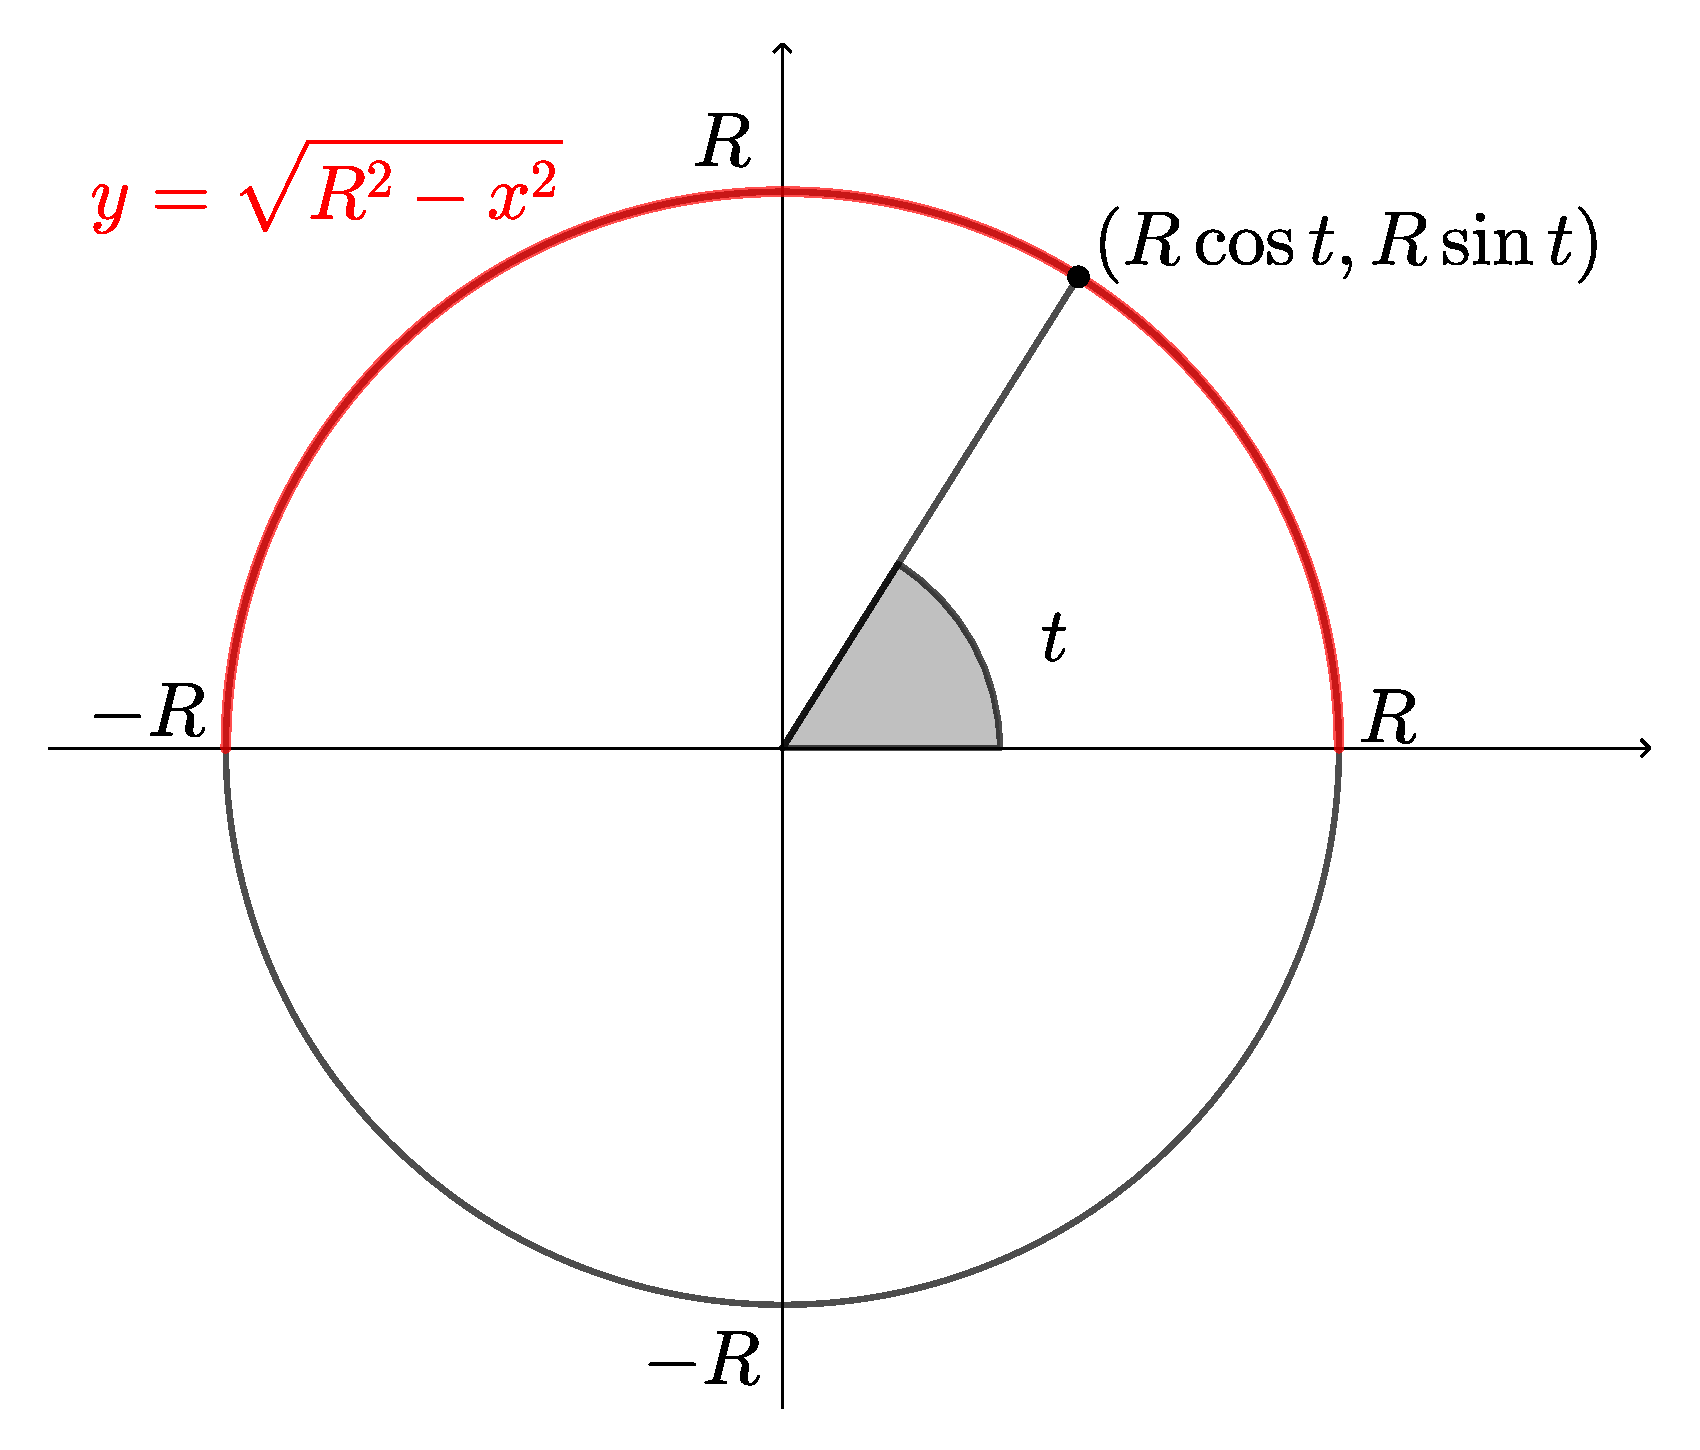
\includegraphics[height=5cm]{05/circle_par.pdf}
    \caption{}
    \label{fig:circle_par}
  \end{figure}
  
  
\end{example}

\begin{example}\label{exmp:parab-length}
  放物線 $y=x^2$ の $0 \leqq x \leqq 1$ の部分の長さ $L$ は定理\ref{thm:lengraph}より以下のように求められる.
  \[
    \begin{aligned}
      L&=\int_{0}^{1} \sqrt{ 1 + \left( \left( x^2\right)'\right)^2}\ dx 
         = \int_{0}^{1} \sqrt{1+4x^2}\ dx
         = \frac{1}{2}\left[ x \sqrt{1+4x^2} + \frac{1}{2} \log \left( 2x+\sqrt{1+4x^2}\right)\right]_{0}^{1}\\
       & = \frac{\sqrt{5}}{2} + \frac{1}{4} \log \left( 2+\sqrt{5} \right)
    \end{aligned}
  \]
  \begin{figure}[h]
    \centering
    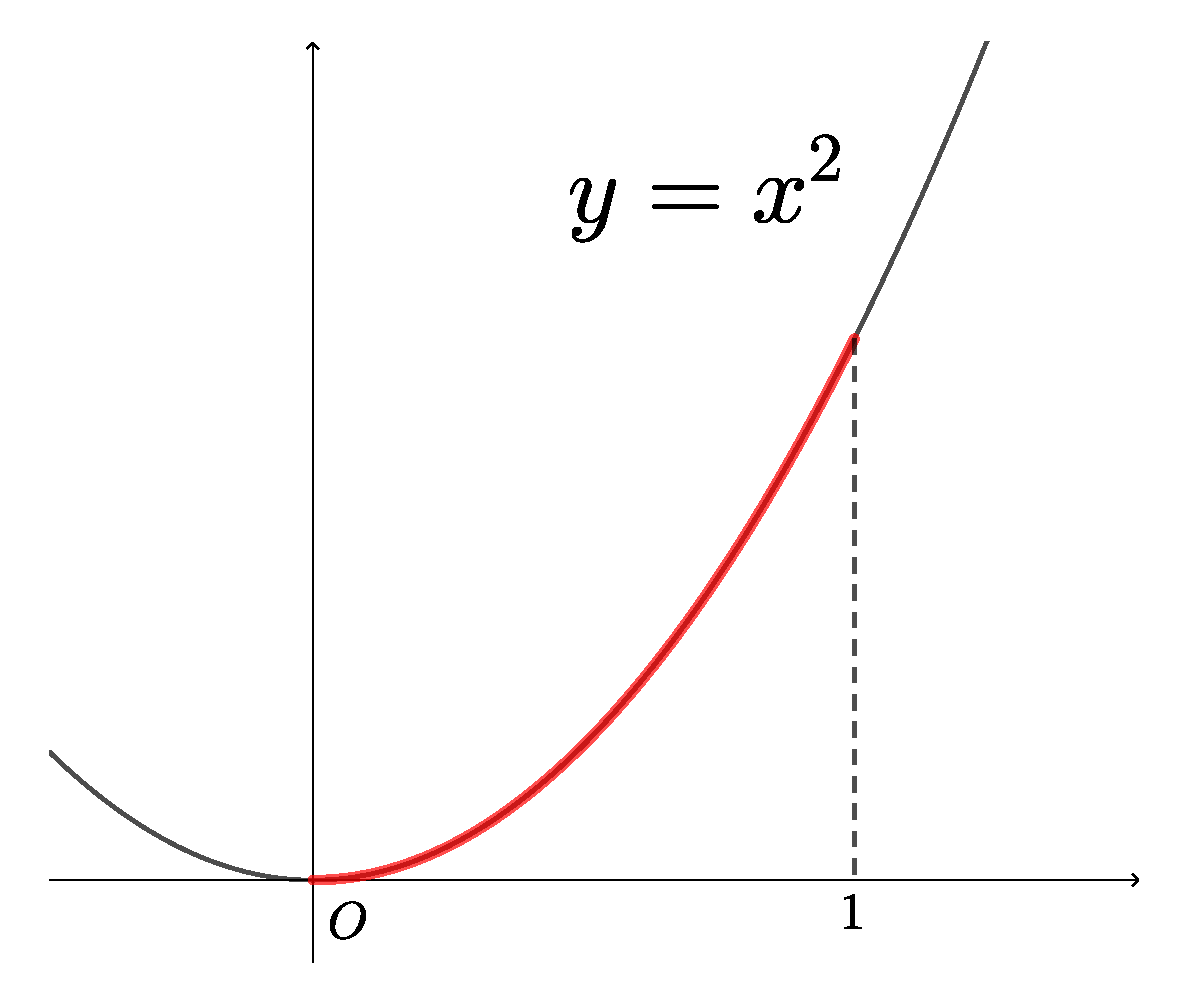
\includegraphics[height=5cm]{05/parab.pdf}
    \caption{放物線 $y=x^2$}
  \end{figure}
\end{example}

\newpage

\subsection{空間曲線の長さと積分}

$\varphi, \psi, \chi$ を閉区間 $[a,b]$ 上定義された $C^1$ 級関数とする.
変数 $t$ が $a$ から $b$ まで動くとき,空間の点 $(\varphi(t), \psi(t),
\chi(t))$ はなめらかな空間曲線 $C$ を描く.これを
\[
  x=\varphi(t), \quad y=\psi(t), \quad z=\chi(t), \quad a \leqq t \leqq b
\]
と書き,空間曲線 $C$ の媒介変数表示という.平面曲線と同様に,空間曲線 $C$ の長さは以下の
積分に等しい.
\[
  \int_{a}^{b} \sqrt{ {\varphi'(t)}^2 + {\psi'(t)}^2 + {\chi'(t)}^2} \ dt
\]

\begin{example}
  常螺旋曲線
  \[
    x=\cos t, \; y=\sin t, \; z=t, \; 0 \leqq t \leqq 2\pi
  \]
  の長さは以下の積分で求められる.
  \begin{align*}
    \int_{0}^{2\pi} \sqrt{ \left( \left( \cos t\right)'\right)^2 + \left( \left( \sin t\right)'\right)^2 
        + \left( t'\right)^2} \ dt
        = \int_{0}^{2\pi} \sqrt{2} \ dt = 2\sqrt{2} \pi
  \end{align*}
  \begin{figure}[h]
    \centering
    \includegraphics[width=10cm]{05/spiral.png}
  \end{figure}
\end{example}

平面曲線は $\bm{r}(t) = \left( x(t), y(t) \right)$ と表せる.また,空間
曲線は $\bm{r}(t) = \left( x(t), y(t), z(t)\right)$ と表せる.平面曲線
に対して $\bm{r}'(t)=\left( x'(t), y'(t)\right)$ とし,空間曲線に対し
て $\bm{r}'(t)=\left( x'(t), y'(t), z'(t)\right)$ とすれば,いずれもの
その長さは以下のように統一的に表せる.
\[
  \int_{a}^{b} \left| \bm{r}'(t)\right| \ dt
\]

\subsection{練習問題}

\begin{enumerate}

\item 曲線 $y=\sin x$ と $y=\cos x$ で囲まれる下図斜線部分の図形の
  面積を求めよう.
  \begin{figure}[h]
    \centering
    
\includegraphics[height=4.5cm]{05/sincos.pdf}
  \end{figure}
  
\item 次の曲線の長さを求めよう.
  \vspace{1zh}
  
  \begin{enumerate}[(1)]

    
  \item $\begin{cases}
      x=t-\sin t\\
      y=1-\cos t
    \end{cases}\quad (0 \leqq t \leqq \pi)$
    \begin{figure}[h]
      \centering
      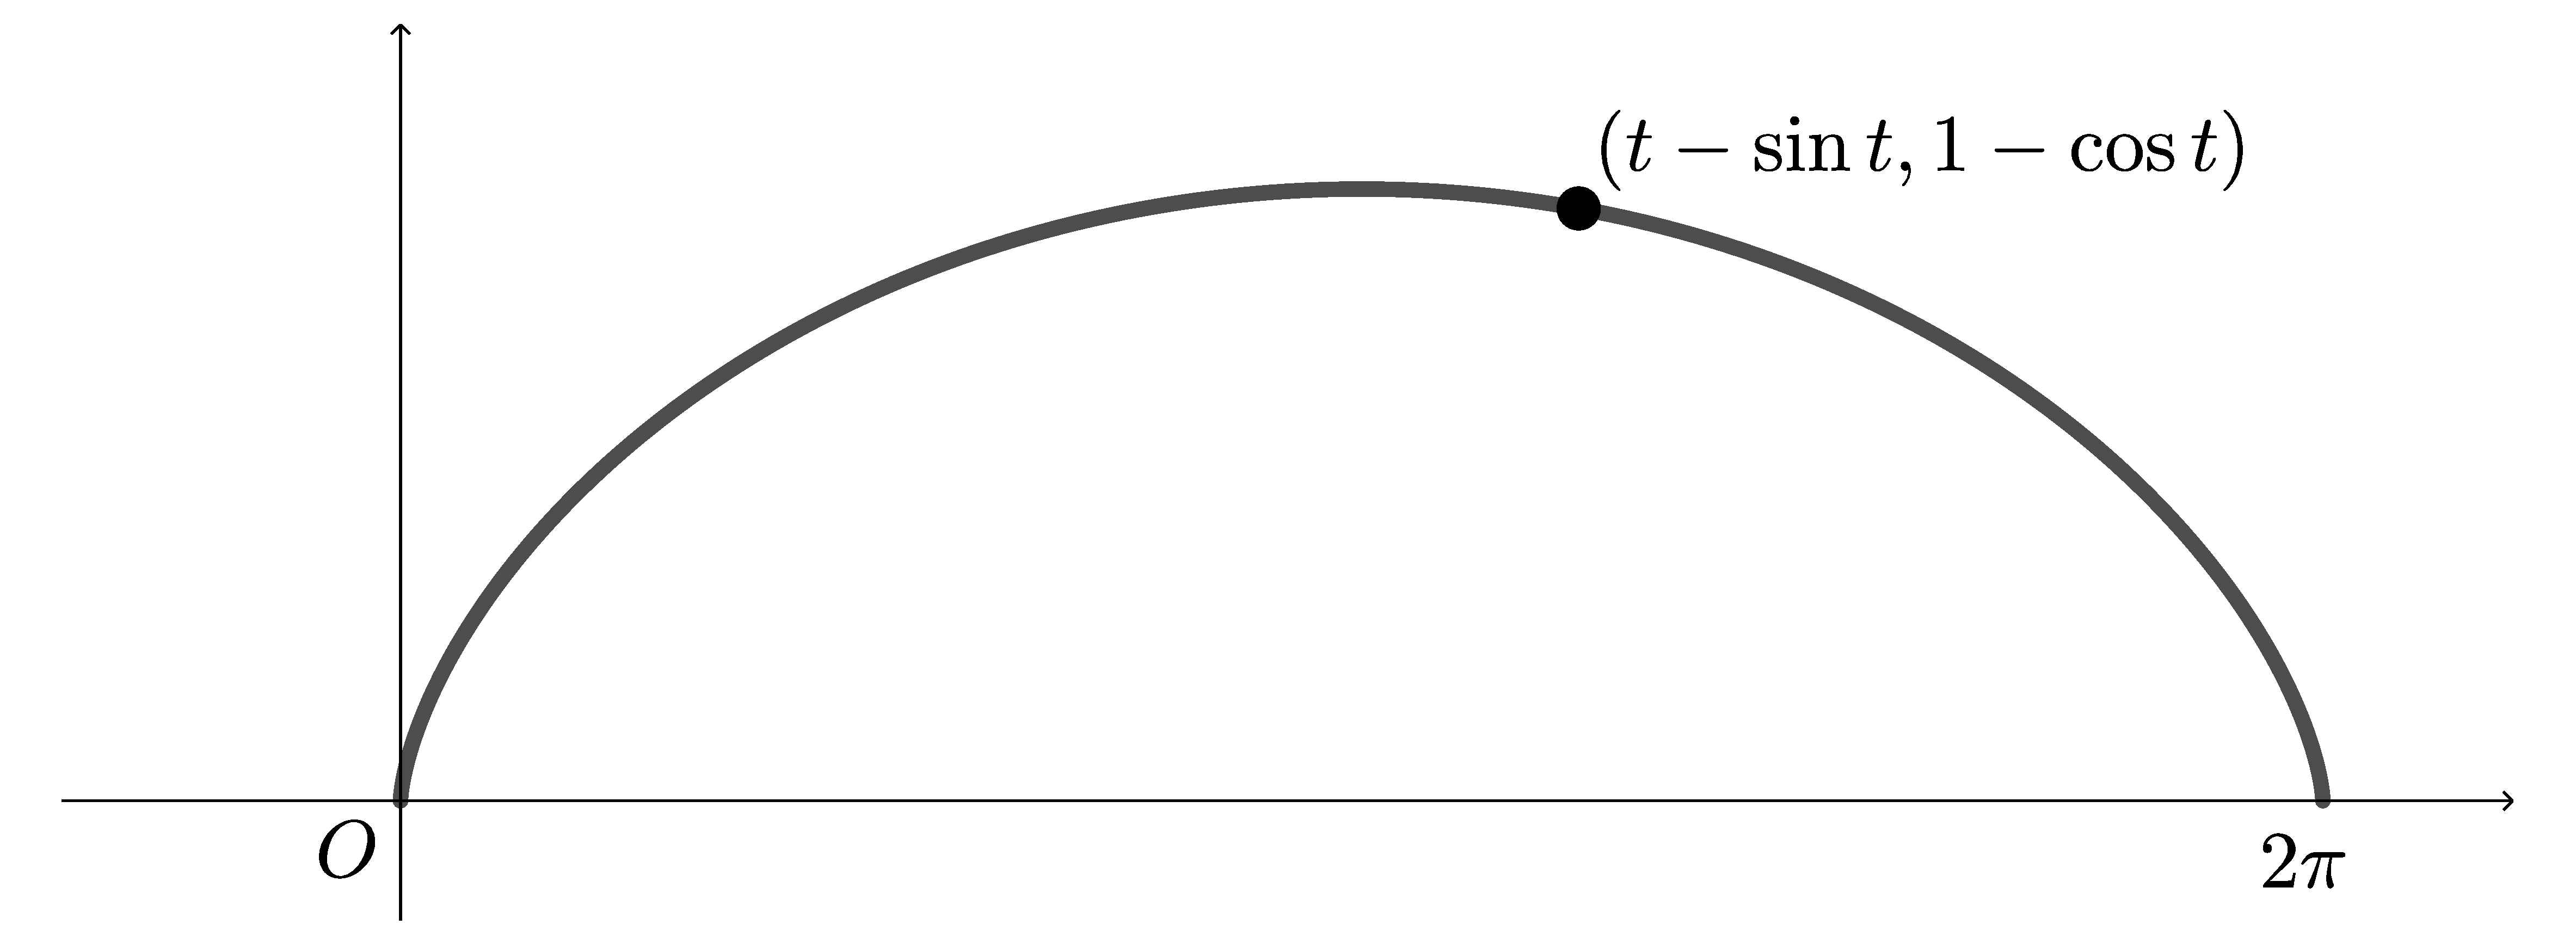
\includegraphics[height=4.5cm]{05/cycloid.pdf}
    \end{figure}
    
  \item $\ds y=\frac{e^{x}+e^{-x}}{2} \; \left(= \cosh x\right) \quad (0 \leqq x \leqq \log 2)$
    \begin{figure}[h]
      \centering
      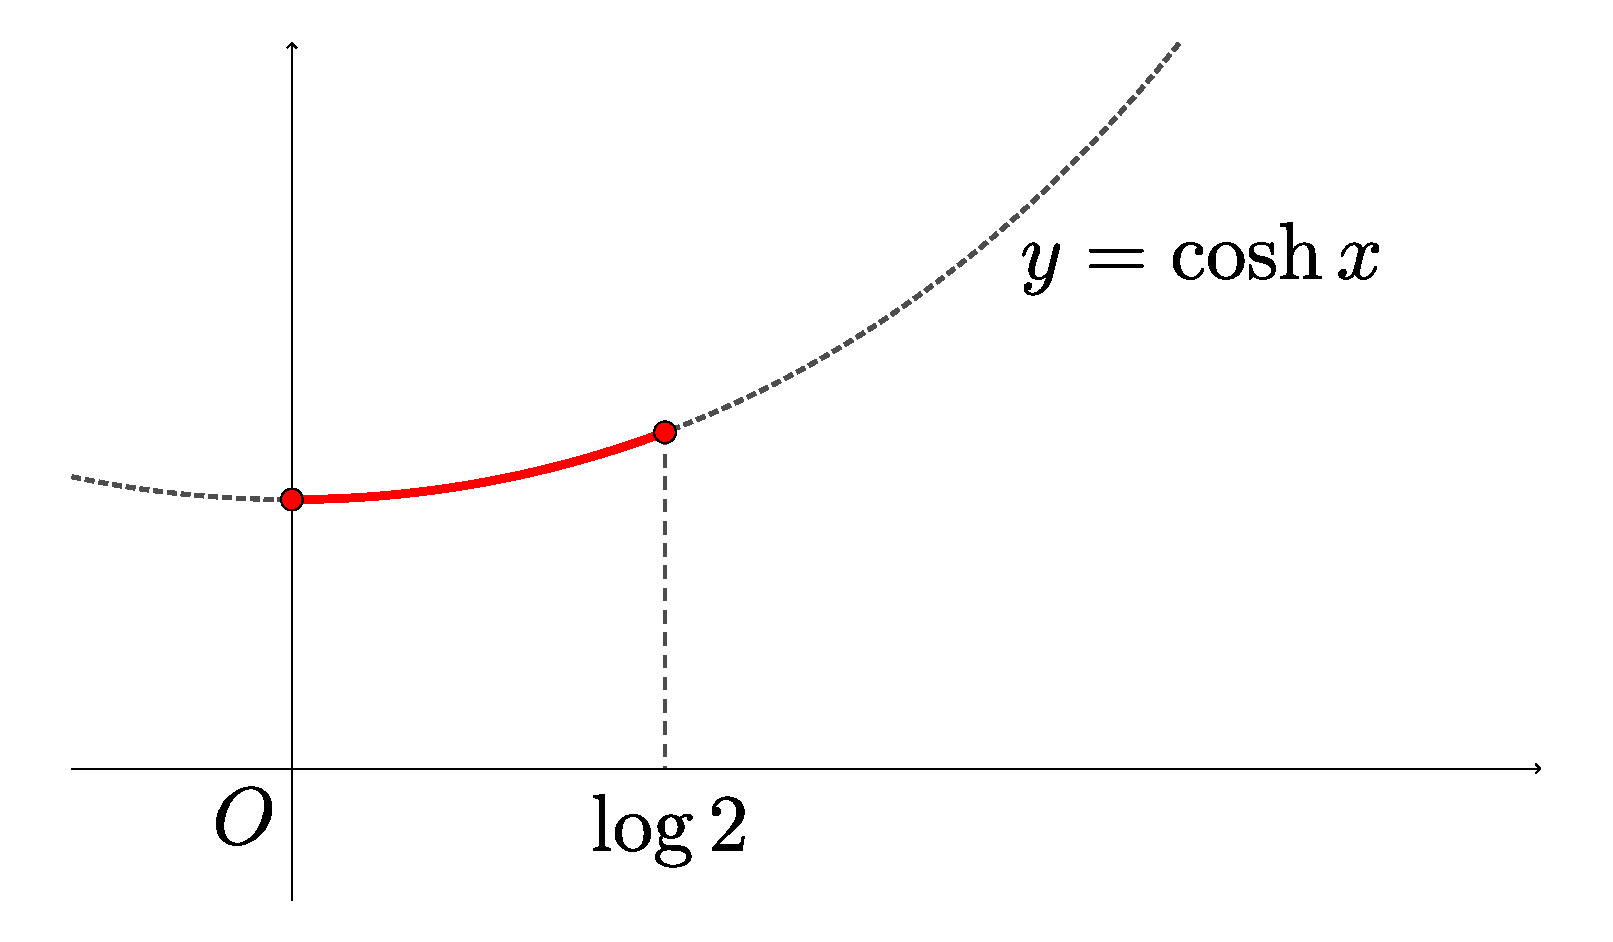
\includegraphics[height=4.5cm]{05/cosh.pdf}
    \end{figure}
  \end{enumerate}
  
  \begin{figure}[b]
  答え : 1. $2\sqrt{2}$ \qquad 2. (1) $4$ \quad (2) $\frac{3}{4}$
\end{figure}

\end{enumerate}

\subsection{(おまけ)平方根を含む関数の積分と双曲線関数}

例えば
\[
  \int \frac{dx}{\sqrt{a^2+x^2}} \quad \text{ や } \quad \int \sqrt{a^2+x^2} \ dx
\]
ような平方根を含む関数の積分には,$u=x+\sqrt{a^2+x^2}$ とおいて置換積
分を使うという自力で見出すのはやや困難な方法がある.それを紹介してもよ
いが,どうせならより自力で見出しにくい方法を紹介しておく.\\

以下の $3$ 個の関数は\textbf{双曲線関数}と呼ばれる.
\[
  \sinh x := \frac{e^{x}-e^{-x}}{2} \qquad \cosh x := \frac{e^{x}+e^{-x}}{2} \qquad
  \tanh x:=\frac{\sinh x}{\cosh x} = \frac{e^{x}-e^{-x}}{e^{x}+e^{-x}}
\]
それぞれ,hyperbolic sine, hyperbolic cosine, hyperbolic tangent と読む.
三角関数の記号 $\sin, \cos, \tan$ とよく似ているが全く別の関数である.
それでいて三角関数に非常によく似た性質を持っている.例えば
\[
  \cosh^2 x - \sinh^2 x =1, \qquad 1 - \tanh^2 x = \frac{1}{\cosh^2x}
\]
という関係式が成り立つことが定義から容易に確かめられる.さらには,三角
関数の加法定理によく似た公式
\[
  \sinh(x \pm y) = (\sinh x)(\cosh y) \pm (\cosh x)(\sinh y), \quad
  \cosh(x \pm y) = (\cosh x)(\cosh y) \pm (\sinh x)(\sinh y)
\]
を定義から容易に導ける.符号の反転が起こらないので,三角関数の公式より
も覚えやすい.三角関数の加法定理が倍角・半角の公式を導くのと全く同様に,
これらは双曲線関数に関する類似の公式
\[
  \begin{aligned}
    &\sinh(2x) = 2 (\sinh x)(\cosh x), \qquad \cosh(2x) = \cosh^2 x +
      \sinh^2 x = 2\cosh^2 x -1 = 1+2\sinh^2 x\\[1ex]
    &\cosh^2(x) = \frac{1+\cosh(2x)}{2}, \qquad \sinh^2 x = \frac{\cosh(2x)-1}{2}
  \end{aligned}
\]
などを導く.さらには,各々の導関数に関しても
\[
  \left( \sinh x \right) = \cosh x, \quad \left( \cosh x \right)' = \sinh x, \quad
  \left( \tanh x\right)' = \frac{1}{\cosh^2x} = 1 - \tanh^2 x
\]
となることもやはり定義から容易に確認できる.これらから積分の公式
\[
  \int \sinh x \ dx = \cosh x, \quad \int \cosh x \ dx = \sinh x,
  \quad \int \frac{dx}{\cosh^2 x} = \tanh x
\]
も導かれる.いずれも三角関数間の関係式とよく似ているが,符号の反転が起きないので覚えやすい.\\

また,逆三角関数が $\sin^{-1}, \cos^{-1}, \tan^{-1}$ と書かれるように,
双曲線関数においても $\sinh^{-1}, \cosh^{-1}, \tanh^{-1}$ は逆数ではな
く,各々の逆関数を表す.その導関数は逆関数の微分公式を使って逆三角関数
と同様に計算できる.例えば $y=\sinh^{-1}x$ の導関数であれば,$x=\sinh
y$ なので
\[
  \left( \sinh^{-1}x \right)'= \frac{dy}{dx} = \frac{1}{\frac{dx}{dy}}
  = \frac{1}{\cosh y} = \frac{1}{\sqrt{1+\sinh^2y}} =
  \frac{1}{\sqrt{1+x^2}}
\]
と計算できる.これは以下の積分の公式を導く.
\[
  \int \frac{dx}{\sqrt{1+x^2}} = \sinh^{-1}x \quad \Bigg( = \log \left( x + \sqrt{1+x^2}\right) \Bigg)
\]
\newpage

長々と語った双曲線関数の一連の性質を使って,例として以下の積分公式を導出する.
\begin{equation}\label{eq:int-sqrt-sinh}
  \int \sqrt{a^2+x^2} \ dx = \frac{1}{2}\left( a^2 \log \left(x+\sqrt{a^2+x^2}\right) + x \sqrt{a^2+x^2} \right) \quad (a>0)
\end{equation}
突然だが
$\ds x= a \sinh u \; \left( \Leftrightarrow u =
  \sinh^{-1}\frac{x}{a}\right)$ とおく.$\ds \frac{dx}{du} = a \cosh
u$ なので
\begin{equation}\label{eq:x-asinh}
  \begin{aligned}
    \int \sqrt{a^2+x^2} \ dx
    &= \int a \sqrt{1+\sinh^2 u}~ \frac{dx}{du}\ du
      = \int a \sqrt{\cosh^2 u}~ \left( a \cosh u\right) \ du
      = a^2 \int \cosh^2 u \ du\\[1ex]
    &= a^2 \int \frac{1+\cosh(2u)}{2} \ du = a^2\left( \frac{u}{2} + \frac{1}{4}\sinh(2u) \right)
      = a^2 \left( \frac{u}{2} + \frac{(\sinh u)(\cosh u)}{2}\right)\\[1ex]
    & = \frac{a^2}{2}\left( u + \left( \sinh u\right) \sqrt{1+\sinh^2 u}\right)
      =\frac{a^2}{2}\left( \sinh^{-1}\frac{x}{a} + \frac{x}{a} \sqrt{1+ \left(\frac{x}{a}\right)^2}\right)\\[1ex]
    & = \frac{1}{2}\left( a^2 \sinh^{-1}\frac{x}{a} + x \sqrt{a^2+x^2}\right)
  \end{aligned}
\end{equation}
である.前ページで紹介した諸々の公式を随所で使いまくっている.ここで,$\ds y=\sinh^{-1}\frac{x}{a}$ とおけば
\[
  y = \sinh^{-1}\frac{x}{a} \; \Longleftrightarrow \; \frac{x}{a} =
  \sinh y = \frac{e^{y}-e^{-y}}{2} \; \Longleftrightarrow \;
  a \left( e^y\right)^2 -2x e^y - a=0
\]
である.最後の等式を $e^y$ に関する2次方程式として解けば,$e^y >0$ と合わせて
\[
  e^y = \frac{x + \sqrt{a^2+x^2}}{a} \quad \text{ より }  \quad y = \log \left( x + \sqrt{a^2+x^2}\right) - \log a
\]
である.(\ref{eq:x-asinh})の最後の $\ds \sinh^{-1}\frac{x}{a}$ をこ
の $y$ に置き換えて,定数 $\ds -\frac{a^2}{2}\log a$ を積分定数に吸収させれば (\ref{eq:int-sqrt-sinh}) が得られる.\\

例\ref{exmp:parab-length}で以下の積分公式をさりげなく使った.
\[
  \int \sqrt{1+4x^2} \ dx = \frac{1}{2}\left(\frac{1}{2} \log \left( 2x + \sqrt{1+4x^2}\right) + x \sqrt{1+4x^2}\right)
\]
これは(\ref{eq:int-sqrt-sinh}) で $\ds a=\frac{1}{2}$ とすれば得られる.実際,
\[
  \int \sqrt{ \left( \frac{1}{2}\right)^2 + x^2 } \ dx = \int
  \sqrt{\frac{1+4x^2}{4}} \ dx = \frac{1}{2}\int \sqrt{1+4x^2} \ dx
\]
なので,$\ds a=\frac{1}{2}$ のときの(\ref{eq:int-sqrt-sinh})を $2$ 倍す
ればよい.なお,定数の差は積分定数が吸収してくれる.\\

この他にも双曲線関数によって計算しやすくなる積分がいくつかある.双曲線
関数やそれにまつわる積分についてより詳しく知りたければ以下の記事を読ん
でみてください.
\begin{center}
  双曲線関数について : \url{https://github.com/kazutsumi/hyperbolic/blob/main/hyperbolic.pdf}
\end{center}



\end{document}


\documentclass[10pt, uplatex, dvipdfmx]{jsarticle}
\usepackage{../mypackage}

\graphicspath{{../pictures}}

\setcounter{section}{5}

\begin{document}

\section{べき級数}

\subsection{級数}

数列 $\{a_n\}$ によって定まる以下の形の式を\textbf{級数}という.
\[
  \sum_{n=0}^{\infty} a_n = a_0+a_1+a_2+ \cdots + a_n + \cdots
\]
以下の $n$ 番目までの部分和 $S_n$ が収束するとき,級数 $\ds
\sum_{n=0}^{\infty} a_n$ は\textbf{収束する}という.
\[
  S_n=\sum_{k=0}^{n}a_n = a_0 + a_1 + \cdots + a_n
\]
また,$\ds \lim_{n \to \infty} S_n = \alpha$ であるとき,級数
$\ds \sum_{n=0}^{\infty}a_n$ の値は $\alpha$
であるといい,$\ds \sum_{n=0}^{\infty} a_n = \alpha$ と書く.当たり前の
ことを長々と定義しているように見えるかもしれないが,例えば
\[
  \sum_{n=0}^{\infty}  (-1)^n = 1 +(-1) + 1 + (-1) + 1 + \cdots
\]
という数列 $\{(-1)^n\}$ から定まる級数を
\[
  \left( 1 + \left(-1\right)\right) + \left(1 + \left(-1\right)\right) + \cdots = 0
\]
と見なしたり
\[
  1 + \left(-1+1\right) + \left(-1+1\right) + \cdots =1
\]
と見なしたりしていては収束先が定まらないので,「前から順番に足す」とい
う約束をしている.この定義に従えば,上の級数は収束しない.

\begin{example}\label{exmp:geo-seq}
  初項が $a$ で公比が $r$ の等比数列の $n$ 番目までの和は
  \[
    \sum_{k=0}^{n}ar^{k} =
    \begin{cases}
      \dfrac{a(1-r^{n+1})}{1-r} & (r \neq 1)\\ \\
      a(n+1) & (r =1)
    \end{cases}
  \]
  なので,等比級数 $\ds \sum_{n=0}^{\infty} a r^{n}$ は $|r|<1$ のとき収束し,その値は
  \[
    \sum_{n=0}^{\infty} ar^{n} = \frac{a}{1-r} \quad (r <1)
  \]
  である.$|r|\geqq 1$ のとき,この等比級数は発散する.
\end{example}

\newpage

\begin{remark}
以後,混乱のおそれがないところでは $\ds \sum_{n=0}^{\infty}$ を単に $\sum$ と略して書く.
\end{remark}

\begin{theorem}[\textbf{級数の和・定数倍}]\label{thm:linear} 2つの級数
  $\sum a_n, \; \sum b_n$ が収束する
  とき,任意の定数 $k, l \in \mathbb{R}$ に対して,級数
  $\ds \sum \left(k a_n+ lb_n\right)$ も収束し,以下が成り立つ.
  \[
    \sum \left( k a_n + l b_n\right)
    = k\left( \sum a_n\right) + l \left(\sum  b_n\right)
  \]
\end{theorem}

\begin{theorem}\label{thm:seq0}
  級数 $\ds \sum a_n$ が収束するなら,数
  列 $\{a_n\}$ は $0$ に収束する.
\end{theorem}

\begin{proof}
  級数 $\ds \sum  a_n$ が $\alpha$
  に収束するとし,$\ds S_n=\sum_{k=0}^{n}a_n$ とすると,$\ds \lim_{n \to \infty}S_n=\alpha$ だから
  \[
    a_n = S_n - S_{n-1}  \to \alpha - \alpha =0 \quad (n \to \infty)
  \]
  より,数列 $\{a_n\}$ は $0$ に収束する.
\end{proof}

定理\ref{thm:seq0}の逆は成り立たない.つまり,数列 $\{a_n\}$ が $0$ に
収束しても級数 $ \sum a_n$ が収束するとは限らない.

\begin{example}\label{exmp:harmonic}
  $a_n=\dfrac{1}{n}$ とすると,数列 $\{a_n\}$ は $0$ に収束する.一方,任意の自然数 $N$ に対して
  \[
    \sum_{n=1}^{N}a_n=\sum_{n=1}^{N} \frac{1}{n}
    \geqq \int_{1}^{N}\frac{dx}{x} = \log N \to \infty \quad (N \to \infty)
  \]
  より,級数 $\sum a_n$ は発散する.なお,部分和 $\ds \sum_{n=1}^{N} a_n$ は下図の灰色部分の面積に等しい.
  \begin{figure}[h]
    \centering
    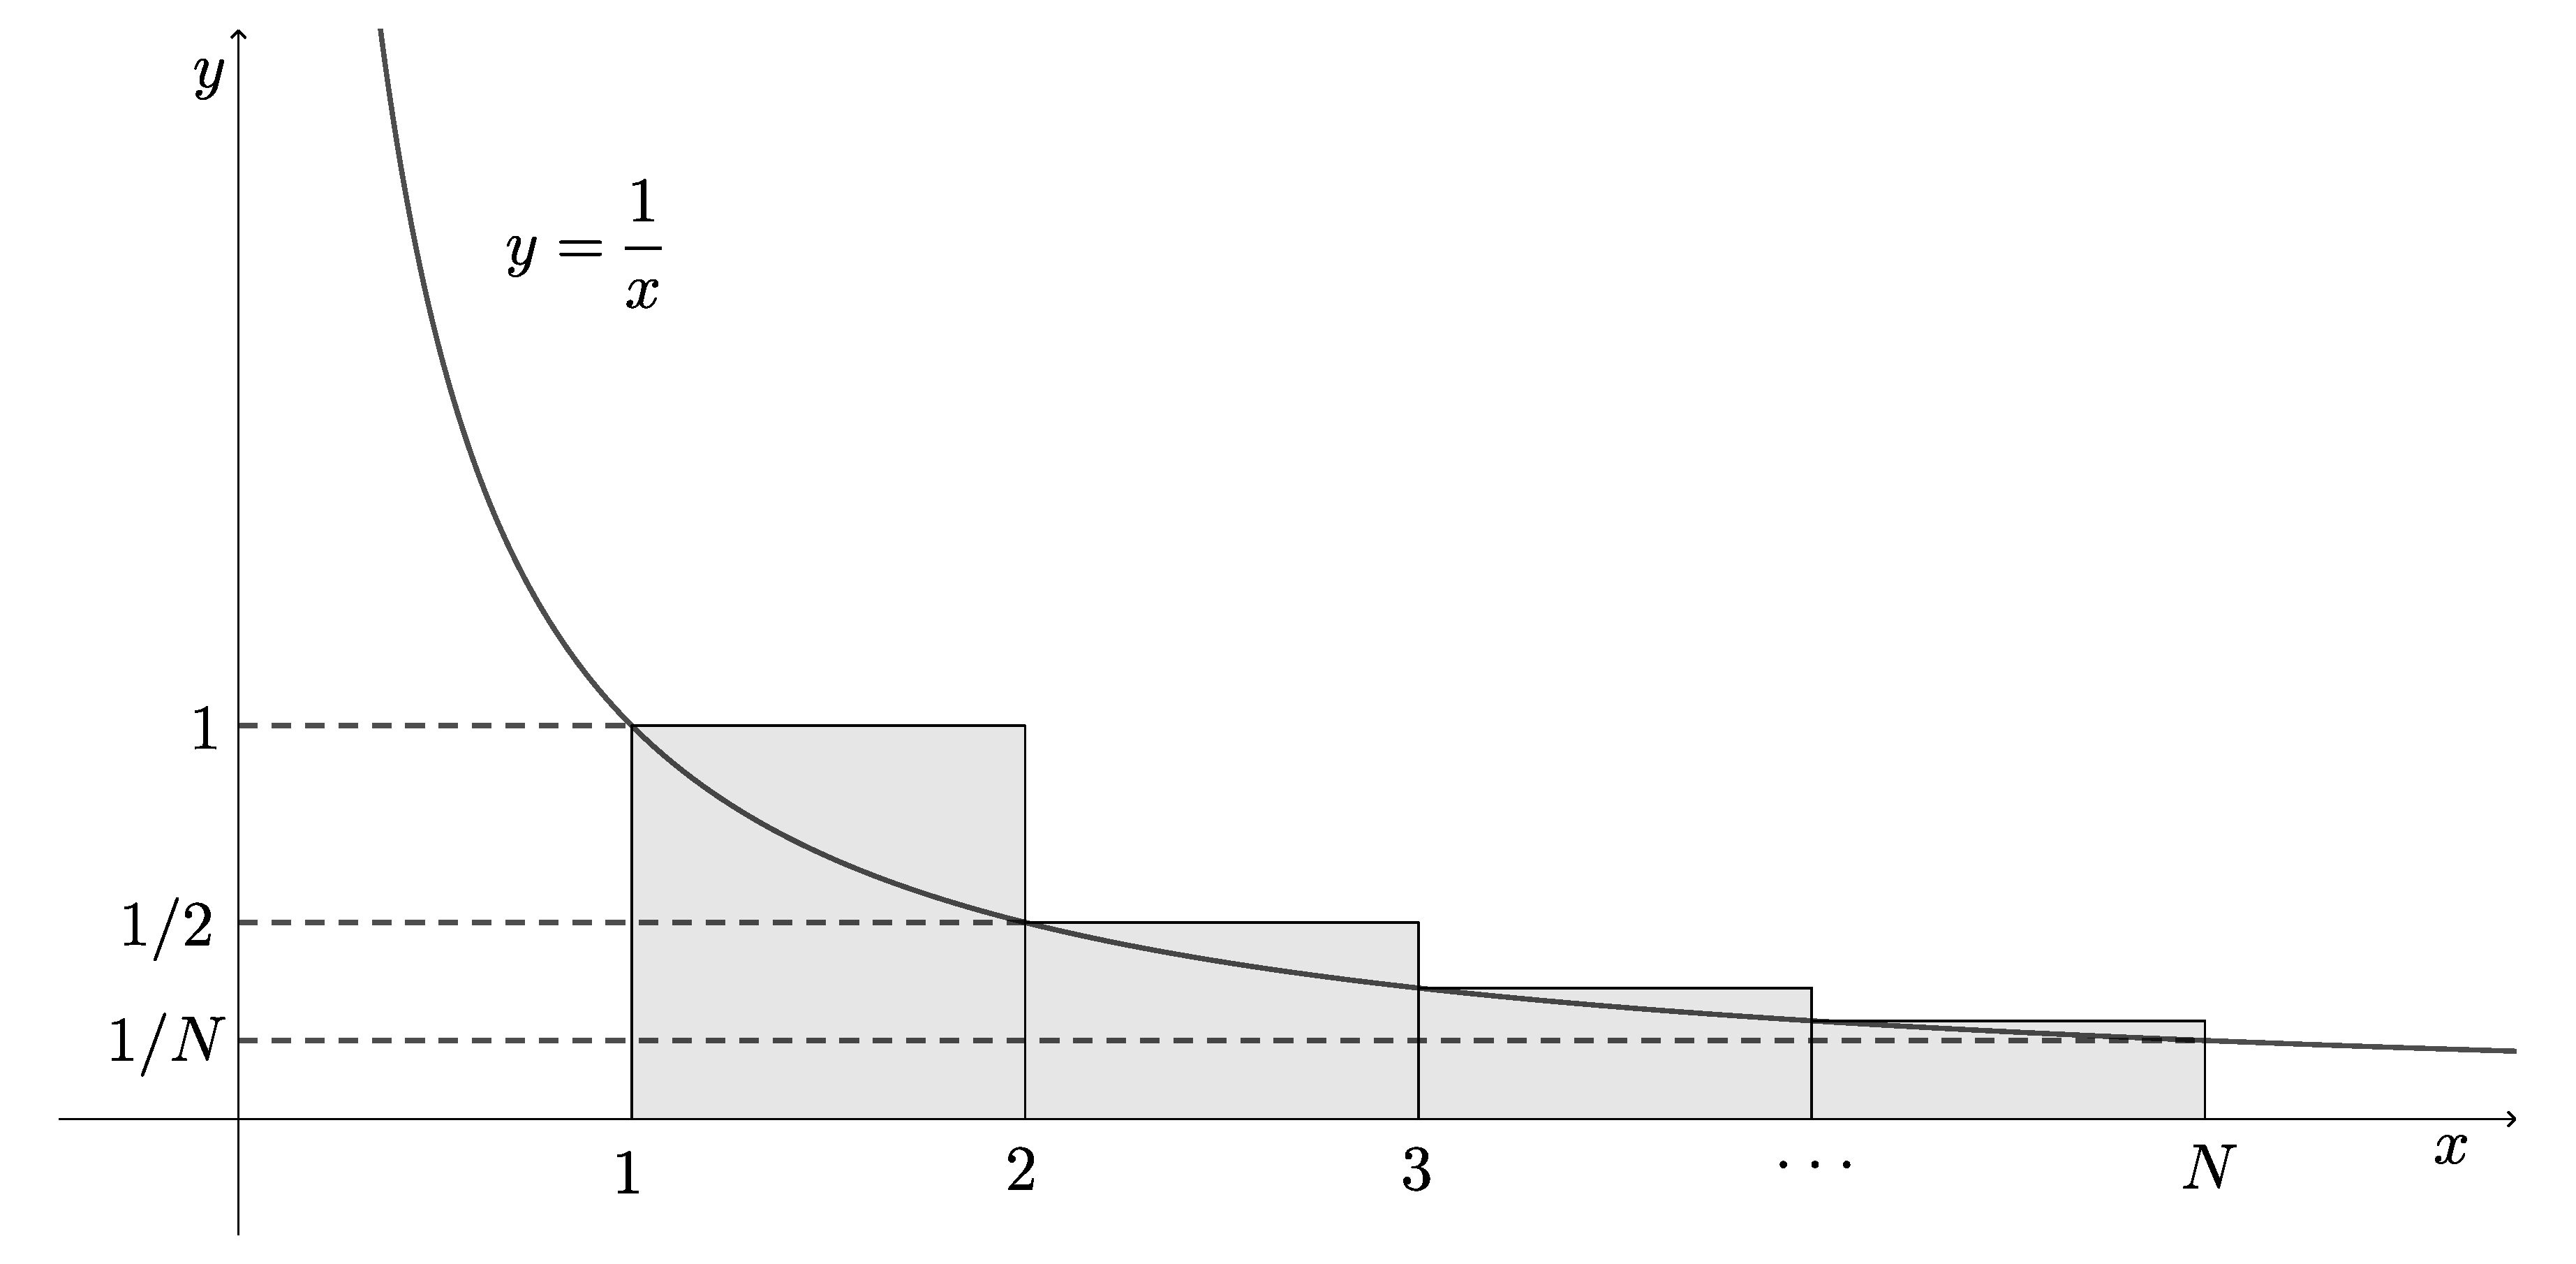
\includegraphics[width=15cm]{06/harmonic.pdf}
  \end{figure}
\end{example}

\newpage
\subsection{べき級数}

数列 $\{a_n\}$ と実数 $b$ と変数 $x$ によって
\[
  \sum_{n=0}^{\infty} a_n(x-b)^n = a_0 + a_1(x-b) + a_2(x-b)^2 + a_3(x-b)^3 + \cdots
\]
と表される級数を,$x=b$ を中心とする\textbf{べき級数}という.$t=x-b$ とおけば,この級数は
\[
  \sum_{n=0}^{\infty} a_n t^n = a_0 + a_1 t + a_2 t^2 + a_3 t^3  + \cdots
\]
と $t=0$ を中心とするべき級数に書き換えられるので,この形のべき級数が重要である.

\begin{example}
  多項式 $a_0 + a_1 x + \cdots +a_n x^n$ は,$a_{k} = 0 \; (k >n)$ とし
  て,べき級数とみなせる.
\end{example}

\begin{definition}[\textbf{Taylor 級数}]
  実数 $a$ を含む開区間 $I$ で $C^{\infty}$ 級な関数 $f$ に対し,
  \[
    \sum_{n=0}^{\infty} \frac{f^{(n)}(a)}{n!}(x-a)^n = f(a) + f'(a)(x-a) + \frac{f''(a)}{2!}(x-a)^2
    + \frac{f^{(3)}(a)}{3!}(x-a)^3 + \cdots
  \]
  を $f$ の $x=a$ を中心とする\textbf{Taylor 級数}という.
\end{definition}

関数 $f$ が $x=a$ でTaylor展開可能なとき,$a$ の近くの $x$ におい
て $f$ の $x=a$ を中心とするTaylor級数は収束し,その値は $f(x)$ に等し
い.しかしながら,一般には $f$ が $C^{\infty}$ 級であってもそのTaylor級数
と $f(x)$ が等しいとは限らない.

\begin{example}
  以下の関数 $f$ の $x=0$ を中心とするTaylor級数を考えてみよう.
  \[
    f(x) =\left\{
      \begin{array}{cc}
        e^{-\frac{1}{x^2}} & (x \neq 0)\\
        0 & (x=0)
      \end{array}
    \right.
  \]
  まず,$f'(0)$ を求めよう.以下は途中で $h=\frac{1}{t}$ と変数変換している.
  \[
    f'(0)=\lim_{h \to 0} \frac{f(0+h)-f(0)}{h} = \lim_{h \to 0} \frac{e^{-\frac{1}{h^2}}}{h}
    = \lim_{t \to \pm \infty} \frac{t}{e^{t^2}} = 0
  \]
  次に,$f''(0)$ を求めよう.やはり以下でも途中で $h=\frac{1}{t}$ と変数変換している.
  \[
    f''(0) = \lim_{h \to 0} \frac{f'(0+h)-f'(0)}{h} = \lim_{h \to 0} \frac{2h^{-3}e^{-\frac{1}{h^2}}}{h}
    =\lim_{t \to \pm \infty} \frac{2t^4}{e^{t^2}} =0
  \]
  以下,同様に計算して $f(0)=f'(0)=f''(0)= f^{(3)}(0)= \cdots = 0$ とな
  ることがわかる.従って,$f$ の $x=0$ のまわりでのTaylor級数は
  \[
    \sum_{n=0}^{\infty} \frac{f^{(n)}(0)}{n!}x^n = 0 + 0x + 0x^2 + \cdots = 0
  \]
  であるが,これは明らかに $x=0$ 以外の全ての $x$ に対して $f(x)$ と等しくない.
\end{example}

\subsection{収束半径}

\begin{theorem}\label{thm:conv-seriese}
  べき級数 $\sum a_n x^n$ が $x=b \; (\neq 0)$ で収
  束するなら,$|x| < |b|$ を満たす全ての $x$ で収束する.
\end{theorem}

\begin{proof}
  級数 $\sum a_n b^n$ が収束するので,数
  列 $\{a_nb^n\}$ は $0$ に収束する.特に,数列 $\{a_n b^n\}$ は上にも
  下にも有界なので,全ての番号 $n \geq 0$ で $|a_n b^n| <M$ となる正の
  実数 $M$が存在する.このとき,各 $x$ に対して $\ds
  r=\left|x/b\right|$ とすると,
  \[
    |a_n x^n| = \left| a_n b^n \cdot \frac{x^n}{b^n}\right| \leq M r^n
  \]
  が成り立つ.従って,$|x| < |b|$ すなわち $r<1$ ならば,級数
  $\sum Mr^n$ が収束するので
  $\sum |a_n x^n|$
  も収束する.よって,$\sum  a_n x^n$ は収束す
  る.
\end{proof}

\begin{remark}
上の証明の終盤では以下の優級数定理と呼ばれる定理を使った.
\end{remark}

\begin{theorem}[\textbf{優級数定理}] 全ての $n$ で $0 \leqq a_n \leqq
  b_n$ であり,級数 $\sum b_n$ が収束するなら,級数 $\sum a_n$ も収束す
  る.このような級数 $\sum b_n$ は級数 $\sum a_n$ の\textbf{優級数}と呼ばれる.
\end{theorem}

\begin{remark}
  級数 $\sum |a_n|$ が収束するとき,級数 $\sum a_n$ は\textbf{絶対収束
    する}という.これは級数 $\sum a_n$ が収束するよりも強い条件である.
  つまり,級数 $\sum a_n$ が絶対収束するなら,$\sum a_n$ は収束する.
\end{remark}

定理\ref{thm:conv-seriese}は級数の発散を判定する以下の定理を導くこともできる.

\begin{theorem}\label{thm:div-seriese}
べき級数 $\sum a_n x^n$ が $x=b$ で発散するな
ら,$|x| > |b|$ を満たす全ての $x$ で発散する.
\end{theorem}

\begin{proof}
$|u|> |b|$ と
なる $u$ でべき級数が収束するなら,定理\ref{thm:conv-seriese}により $x=b$ でべ
き級数が収束し,$x=b$ で発散することに矛盾する.
\end{proof}


\begin{definition}[\textbf{収束半径}]
  べき級数 $\sum a_n x^n$ が $|x| < r$ のとき収束
  し,$|x|>r$ のとき発散するとき,$r$ をこのべき級数の\textbf{収束半径}と
  いう.ただし,$x=0$ でのみ収束するときは $r=0$ とし,全ての実数 $x$
  で収束するときは $r=+\infty$ と定める.
\end{definition}


\begin{remark}
  収束半径 $r$ が $0 < r < +\infty$ のとき,定
  理\ref{thm:conv-seriese}からべき級数 $\sum  a_n
  x^n$ は $|x| <r$ で収束し,$|x|>r$ で発散する.なお,$x= \pm r$ にお
  ける収束・発散は個別に調べなければわからない.
\end{remark}


\begin{example}\label{exmp:geo}
  べき級数 $\ds \sum_{n=0}^{\infty} x^n$ は $|x|<1$ で絶対収束
  し,$|x|>1$ で発散するから,その収束半径は $1$ である.なお,この場
  合 $x=\pm1$ では発散することが容易にわかる.よって,$|x|<1$ において
  以下が成り立つ.
  \[
    \sum_{n=0}^{\infty}x^n=\frac{1}{1-x}
  \]
\end{example}

\newpage

全ての $n$ で $a_n>0$ となる級数 $\sum a_n$ を\textbf{正項級数}という.

\begin{theorem}[\textbf{Cauchy の収束判定法}]
  正項級数 $\sum a_n$ に対して,$\ds \rho := \lim_{n \to \infty}
  \sqrt[n]{a_n}$ とする.$\rho <1$ なら $\sum a_n$
  は収束し,$\ds \rho >1 \; \left( \lim_{n \to \infty} \sqrt[n]{a_n} =
    \infty \text{ も含む }\right)$ なら $\sum a_n$ は発散する.
\end{theorem}

\begin{theorem}[\textbf{d'Alembert の収束判定法}]
  正項級数 $\sum a_n$
  に対して,$\ds \rho:= \lim_{n \to \infty} \frac{a_{n+1}}{a_{n}}$ とす
  る.$\rho <1$ なら $\sum a_n$
  は収束し,$\ds \rho >1 \; \left( \lim_{n \to \infty} \frac{a_{n+1}}{a_n}
    = \infty \text{ も含む } \right)$ なら $\sum a_n$ は発散する.
\end{theorem}

\begin{remark}
  Cauchy の収束判定法も d'lAmbert の収束判定法も $\rho=1$ となるときに
  は収束・発散に関して何も教えてくれない.その場合は個別に別の方法で調べなければならない.
\end{remark}

\begin{theorem}\label{thm:criterion}
  べき級数 $ \sum a_n x^n$ の収束半径を $r$ とする.
  このとき次が成り立つ.
  \begin{enumerate}[(1)]
    \setlength{\itemsep}{1zh}
  \item 極限値 $\ds l = \lim_{n \to \infty} \sqrt[n]{|a_n|}$ が存在するとき,$\ds r=\frac{1}{l}$ である.
  \item 極限値
    $\ds l = \lim_{n \to \infty} \left| \frac{a_{n+1}}{a_n}\right|$ が
    存在するとき,$\ds r=\frac{1}{l}$ である.
  \end{enumerate}
  ただし,$l=0$ のときは $r=+\infty$ であり,$l=+\infty$ のときは $r=0$ である.
\end{theorem}

\begin{proof}
  \begin{enumerate}[(1)]
    \setlength{\itemsep}{1zh}
    
  \item 実数 $x$ に対して
    $\ds \lim_{n \to \infty} \sqrt[n]{|a_n x^n|} =
    \lim_{n=\infty}\sqrt[n]{|a_n|}|x| = l |x|$ である.従って,Cauchyの
    収束判定法から
    \begin{itemize}
      \setlength{\itemsep}{1zh}
    \item $l |x| <1$ すなわち $|x| < \dfrac{1}{l}$ ならば,べき級数は絶対収束する.
    \item $l |x| >1$ すなわち $|x| > \dfrac{1}{l}$ ならば,級数
      $\sum |a_n x^n|$ は発散する.
    \end{itemize}
    よって,収束半径は $r=\dfrac{1}{l}$ である.

  \item 実数 $x$ に対して
    $\ds \lim_{n \to \infty} \left| \frac{a_{n+1}x^{n+1}}{a_n
        x^n}\right| = \lim_{n \to \infty}
    \left|\frac{a_{n+1}}{a_n}\right| |x| = l |x|$ である.従って,d'Alembertの収束判定法から
    \begin{itemize}
      \setlength{\itemsep}{1zh}
    \item $l|x| <1$ すなわち $|x| < \dfrac{1}{l}$ ならば,べき級数は絶対収束する.
    \item $l|x| >1$ すなわち $|x| > \dfrac{1}{l}$ ならば,級数 $\sum |a_n x^n|$ は発散する.
    \end{itemize}
    よって,収束半径は $r= \dfrac{1}{l}$ である.
  \end{enumerate}
\end{proof}

\begin{example}
  べき級数 $\ds \sum_{n=0}^{\infty} \frac{x^n}{n!}$ の収束半径
  は $+\infty$ である.すなわち,全ての実数 $x$ で収束する.

  実際,$\ds a_n=\frac{1}{n!}$ とおけばこのべき級数は $\ds \sum_{n=0}^{\infty} a_n x^n$ と書けるので,
  \[
    \lim_{n \to \infty} \left| \frac{a_{n+1}}{a_n}\right| = \lim_{n \to \infty} \frac{1}{n+1} = 0
  \]
  より定理\ref{thm:criterion}から収束半径は $+\infty$ である.

\end{example}

\newpage

\subsection{項別積分・項別微分}

べき級数 $\sum a_n x^n$ の収束半径が $r>0$ なら,これは開区間 $(-r,r)$ 上の関数
\[
  f(x) = \sum  a_n x^n = a_0 + a_1 x + a_2 x^2 + \cdots
\]
を定義する.このとき,$f$ は $(-r,r)$ で連続である.

\begin{theorem}[\textbf{項別積分}]\label{thm:term-int}
  べき級数 $f(x) = \sum a_n x^n$ の収束半径を $r>0$
  とする.このとき,開区間 $(-r,r)$ 上で以下が成り立つ.すなわち,右辺の収束半径は $r$ である.
  \[
    \int_{0}^{x} f(t) \ dt = \sum_{n=0}^{\infty} \frac{a_n}{n+1}x^{n+1}
  \]
\end{theorem}

\begin{theorem}[\textbf{項別微分}]\label{thm:term-diff}
  べき級数 $f(x) = \sum a_n x^n$ と
  $g(x) = \sum  na_n x^{n-1}$ に次が成り立つ.
  \begin{enumerate}[(1)]
    
  \item $g(x)$ の収束半径は $f(x)$ の収束半径に等しい.

  \item $f(x)$ の収束半径が $r>0$ のとき,$f$ は $(-r,r)$ で微分
    可能で,$f'(x) = g(x)$ である.
  \end{enumerate}
\end{theorem}

\begin{theorem}
  正の収束半径 $r$ を持つべき級数 $f(x) = \sum  a_n
  x^n$ は $(-r,r)$ で $C^{\infty}$ 級である.
\end{theorem}
\begin{proof}
  定理\ref{thm:term-diff}より $f'(x) = \sum  n a_n
  x^{n-1}$ であり,その収束半径も $r$ である.よって,定
  理\ref{thm:term-diff}を繰り返し適用して,$f$ は何回でも微分できること
  が示せる.
\end{proof}

\begin{theorem}\label{thm:coeff}
  べき級数 $f(x) = \sum  a_n x^n$ が正の収束半
  径 $r$を持つとき,各 $n=0,1,2,\ldots$ に対して以下が成り立つ.
  \[
    a_n = \frac{f^{(n)}(0)}{n!}
  \]
\end{theorem}
\begin{proof}
  $f$ に定理\ref{thm:term-diff}を繰り返し適用して
  \[
    f^{(n)}(x) = n! a_n + \left( (n+1)n \cdots  2\right)a_{n+1} x + \left( (n+2)(n+1)\cdots 3\right) a_{n+2} x^2 + \cdots
  \]
  だから,これに $x=0$ を代入して $f^{(n)}(0) = n! a_n$ を得る.
\end{proof}

\begin{theorem}[\textbf{べき級数展開の一意性}]\label{thm:unique-seriese}
  $C^{\infty}$ 級関数 $f$ が,正の収束半径を持つべき級数として
  \[
    f(x) = \sum  a_n x^n = \sum b_n x^n
  \]
  と2通りに表せたとき,各 $n=0,1,2,\ldots$ に対して $a_n=b_n$ である.
\end{theorem}

\begin{proof}
  定理\ref{thm:coeff}より,各 $n=0,1,2,\ldots$ に対して
  $\ds a_n = \frac{f^{(n)}(0)}{n!} =b_n$ である.
\end{proof}

\newpage

\subsection{Taylor 展開}

実数 $a$ の近くで $C^{\infty}$ 級な関数 $f$ の $n$ 次剰余項
\[
  R_n(x) = f(x) -\sum_{n=0}^{n-1}\frac{f^{(k)}(a)}{k!}(x-a)^{n-1}
\]
が $n \to \infty$ のときに $0$ に収束すると
き,$f$ は $x=a$ で\textbf{Taylor展開可能}であるといい,そのTaylor級
数を $f$ の $x=a$ での\textbf{Taylor展開}という.このとき
\[
  f(x) = \sum_{n=0}^{\infty} \frac{f^{(n)}(a)}{n!}(x-a)^n
\]
である.特に,$a=0$ でのTaylor展開を $f$ の\textbf{Maclaurin展開}という.

\begin{example}\label{exmp:taylor-serieses}
  代表的なMaclaurin展開をいくつか挙げておく.
  \[
    \begin{aligned}
      e^x &= \sum \frac{x^n}{n!} = 1 + x +
            \frac{x^2}{2!} + \frac{x^3}{3!} + \cdots \quad (-\infty < x <
            \infty)\\
      \sin x & = \sum (-1)^n \frac{x^{2n+1}}{(2n+1)!}
               = x - \frac{x^3}{3!} + \frac{x^5}{5!} -\frac{x^7}{7!} + \cdots \quad (-\infty < x < \infty)\\
      \cos x &= \sum (-1)^n \frac{x^{2n}}{(2n)!}
               = 1 - \frac{x^2}{2!} + \frac{x^4}{4!}-\frac{x^6}{6!}+\cdots \quad (-\infty < x < \infty)\\
      (1+x)^{a} &= \sum \binom{a}{n}x^n = 1 + \binom{a}{1}x + \binom{a}{2}x^2
                  + \binom{a}{3}x^3 + \cdots \quad (-1 < x < 1)
        \end{aligned}
      \]
      ただし,最後の級数の係数は一般化二項係数である.
      \[
        \binom{a}{k} := \frac{\overbrace{a(a-1)\cdots(a-k+1)}^{k \text{ 個 }}}{n!}, \qquad \binom{a}{0}:=1
      \]
    \end{example}


\begin{example}\label{exmp:log-taylor}
  例\ref{exmp:geo}のべき級数 $\sum  x^n$ の収束半径
  は $1$ である.従って,$|x|<1$ において
  \[
    \frac{1}{1-x} = \sum x^n = 1 + x + x^2 + x^3 + \cdots 
  \]
  である.べき級数展開の一意性(定理\ref{thm:unique-seriese})からこれは関数 $
  f(x)=\dfrac{1}{1-x}$ のMaclaurin展開でもある.また,$|x|<1$ のと
  き,$|-x|<1$ だから
  \[
    f(-x) = \frac{1}{1+x} = \sum (-x)^n = 1 -x + x^2 - x^3 + \cdots 
  \]
  であり,最右辺の収束半径は $1$ である.よって,項別積分ができて(定理\ref{thm:term-int})
  \[
    \log(1+x) = \int_{0}^{x} \frac{dt}{1+t} = \sum \frac{(-1)^n}{n+1} x^{n+1}
    = x - \frac{x^2}{2} + \frac{x^3}{3} - \frac{x^4}{4} + \cdots 
  \]
  が $|x|<1$ で成り立つ.これは関数 $\log(1+x)$ のMaclaurin展開である.
  ちなみに,このMaclaurin展開は $x=1$ でも成り立つので,
  \[
    \log 2 = 1 - \frac{1}{2} + \frac{1}{3} - \frac{1}{4} + \cdots
  \]
  である.なお,$x=-1$ のとき級数は発散する.
\end{example}

\begin{example}\label{exmp:atan-taylor}
  $\tan^{-1}x$ のMaclaurin展開とその収束半径を項別積分を使って求める.

  例\ref{exmp:log-taylor}で見たように,$|x|<1$ で
  \[
    \frac{1}{1+x} = \sum (-x)^n = 1 - x + x^2 - x^3 + \cdots
  \]
  である.$|x| <1$ のとき,$|x^2|<1$ なので $x$ に $x^2$ を代入して
  \[
    \frac{1}{1+x^2} = \sum(-x^2)^n=\sum (-1)^n x^{2n}
    =1 -x^2 + x^4 - x^6 + \cdots 
  \]
  を得る.この収束半径は $1$ である.よって,項別積分ができて(定理\ref{thm:term-int})
  \[
    \tan^{-1}x = \int_{0}^{x}\frac{dt}{1+t^2} = \sum \frac{(-1)^n}{2n+1}x^{2n+1}
    = x - \frac{x^3}{3} + \frac{x^5}{5} - \frac{x^7}{7} + \cdots
  \]
  が開区間 $(-1,1)$ で成り立つ.べき級数展開の一意性(定理\ref{thm:unique-seriese})からこれ
  は $\tan^{-1}x$ のMaclaurin展開であり,定理\ref{thm:term-int}からその
  収束半径は $1$ である.
\end{example}

\begin{example}\label{exmp:int-exp-x2-taylor}
  以下の関数 $G(x)$ の Maclaulin 展開を項別積分を
  使って求める.
  \[
    G(x) := \int_{0}^{x} e^{-t^2} \ dt
  \]
  例\ref{exmp:taylor-serieses}で挙げた指数関数 $e^x$ の Maclaulin 展開の $x$ に $-t^2$ を代入して以下が得られる.
  \[
    e^{-t^2} = 1 - t^2 + \frac{t^4}{2!} - \frac{t^6}{3!} + \cdots + \frac{(-1)^n}{n!}t^{2n} + \cdots \quad (- \infty < t < \infty)
  \]
  右辺は項別積分ができる(定理\ref{thm:term-int})ので両辺を $0$ から $x$ まで積分して以下を得る.
  \begin{equation}\label{eq:G-seriese}
    G(x) = \int_{0}^{x}e^{-t^2} \ dt = x - \frac{x^3}{3} + \frac{x^5}{10} - \frac{x^7}{42} + \cdots + \frac{(-1)^n}{n! (2n+1)}x^{2n+1} + \cdots
    \quad (- \infty < x < \infty)
  \end{equation}
  べき級数の一意性(定理\ref{thm:unique-seriese})から,これは $G(x)$ の Maclaulin 展開である.\\
 

  
  ちなみに,この関数 $G(x)$ の $\ds \frac{2}{\sqrt{\pi}}$ 倍は\textbf{誤差関数 (error function)}
  と呼ばれ,$\erf(x)$ と書かれる.
  \[
    \erf (x) = \frac{2}{\sqrt{\pi}}\int_{0}^{x} e^{-t^2} \ dt 
  \]
  わざわざ $\ds \frac{2}{\sqrt{\pi}}$ 倍する理由はいずれ説明するつもり
  だが,これは初等関数(多項式,三角関数,逆三角関数,指数関数,対数関
  数,無理関数たちのある種の組み合わせとして表せる関数)でないことが知
  られている.そのため,各 $x$ での関数値を知るのも困難だが,上記の級数
  表示(\ref{eq:G-seriese})によって原理上は任意精度の近似値を計算するこ
  とができる.
\end{example}

\newpage
\subsection{(おまけ)Taylorの定理と積分}

\begin{theorem}\label{thm:taylor-int}
  $f$ を実数 $a$ を含む開区間 $I$ で $C^n$ 級な関数とする.このとき,任
  意の $x \in I$ に対して以下が成り立つ.
  \[
    f(x) = \sum_{k=0}^{n-1} \frac{f^{(k)}(a)}{k!}(x-a)^k +
    \int_{a}^{x}\frac{f^{(n)}(t)}{(n-1)!}(x-t)^{n-1} \ dt
  \]
\end{theorem}

\begin{proof}
  微分積分学の基本定理から,任意の $x \in I$ に対して
  \[
    f(x)-f(a) = \int_{a}^{x} f'(t) \ dt
  \]
  である.右辺の積分に部分積分を繰り返し適用して,以下を得る. 
  \[
    \begin{aligned}
      f(x) &= f(a) + \int_{a}^{x} \left( -(x-t)\right)' f'(t) \ dt\\
      &= f(a) + \Big[\left( -\left(x-t\right)\right)f'(t)\Big]_{t=a}^{t=x} + \int_{a}^{x} f''(t)(x-t)\ dt\\
      &= f(a) + f'(a)(x-a)+ \int_{a}^{x} \left( -\frac{(x-t)^2}{2}\right)' f''(t) \ dt\\
      &= \sum_{k=0}^{1}\frac{f^{(k)}(a)}{k!}(x-a)^k + \left[ -\frac{(x-t)^2}{2!}f''(t)\right]_{t=a}^{t=x}
      + \int_{a}^{x}\frac{f^{(3)}(t)}{2!}(x-t)^2\ dt\\
      &= \sum_{k=0}^{2}\frac{f^{(k)}(a)}{k!}(x-a)^k + \left[-\frac{(x-t)^3}{3!}f^{(3)}(t)\right]_{t=a}^{t=x}
      +\int_{a}^{x} \frac{f^{(4)}(t)}{3!}(x-t)^3 \ dt\\
      &= \sum_{k=0}^{3}\frac{f^{(k)}(a)}{k!}(x-a)^k + \left[-\frac{(x-t)^4}{4!}f^{(3)}(t)\right]_{t=a}^{t=x}
      + \int_{a}^{x} \frac{f^{(5)}(t)}{4!} (x-t)^4 \ dt\\
      &\qquad  \vdots\\
      &= \sum_{k=0}^{n-1}\frac{f^{(k)}(a)}{k!}(x-a)^k
      + \int_{a}^{x} \frac{f^{(n)}(t)}{(n-1)!}(x-t)^{n-1} \ dt
    \end{aligned}
  \]

\end{proof}

上の定理において
\[
  R_{n}(x) := \int_{a}^{x}\frac{f^{(n)}(t)}{(n-1)!}(x-t)^{n-1}\ dt
\]
を積分形の剰余項という.これは Taylor の定理における剰余項の別の表現方
法である.この定理\ref{thm:taylor-int}から Taylor の定理を導くこともできる.


\begin{theorem}[\textbf{Taylor の定理}]\label{thm:taylor}
  定理\ref{thm:taylor-int}と同じ仮定のもとで,任意の $x \in I$ に対して,
  以下を満たす実数 $c$ が存在する.
  \[
    f(x) = \sum_{k=0}^{n-1}\frac{f^{(k)}(a)}{k!}(x-a)^k
    +\frac{f^{(n)}(c)}{n!}(x-a)^n, \quad a<c<x \text{ または } x<c<a
  \]
\end{theorem}

\begin{proof}
  $a>x$ のときも同様に示せるので,$a<x$ とする.定理\ref{thm:taylor-int}から
  \[
    R_n(x):=\int_{a}^{x}\frac{f^{(n)}(t)}{(n-1)!}(x-t)^{n-1}\ dt =
    \frac{f^{(n)}(c)}{n!}(x-a)^n, \quad a<c<x
  \]
  を満たす実数 $c$ が存在することを示せばよい.$f$ は開区
  間 $I$ で $C^n$ 級なので,$f^{(n)}$ は閉区間 $[a,x]$ で連続である.従っ
  て,最大値・最小値の定理から,区間 $[a,x]$ における $f^{(n)}$ の最小
  値 $m$ と最大値 $M$ が存在するので
  \[
    \int_{a}^{x} \frac{m}{(n-1)!}(x-t)^{n-1}\ dt
    \leq R_n(x)
    \leq \int_{a}^{x} \frac{M}{(n-1)!}(x-t)^{n-1}\ dt
  \]
  である.ここで,
  \[
    \begin{aligned}
      \int_{a}^{x}\frac{m}{(n-1)!}(x-t)^{n-1}\ dt
      &= \frac{m}{(n-1)!}\left[ -\frac{(x-t)^{n}}{n}\right]_{t=a}^{t=x}
      =\frac{m}{n!}(x-a)^n\\ 
      \int_{a}^{x}\frac{M}{(n-1)!}(x-t)^{n-1}\ dt
      &=\frac{M}{(n-1)!}\left[ -\frac{(x-t)^{n}}{n}\right]_{t=a}^{t=x}=\frac{M}{n!}(x-a)^n
    \end{aligned}
  \]
  より
  \[
    m \leq \frac{n!}{(x-a)^n} R_n(x) \leq M
  \]
  である.よって,中間値の定理から
  \[
    \frac{n!}{(x-a)^n}R_n(x) =f^{(n)}(c)
  \]
  を満たす実数 $c \in (a,x)$ が存在する.これから以下を得る.
  \[
    R_n(x) = \frac{f^{(n)}(c)}{n!}(x-a)^n
  \]
\end{proof}

Taylor の定理における剰余項
\[
  R_n(x) = \frac{f^{(n)}(c)}{n!}(x-a)^n
\]
はLagrangeの剰余項と呼ばれる.



\end{document}


\documentclass[10pt, uplatex, dvipdfmx]{jsarticle}
\usepackage{../mypackage}

\graphicspath{{../pictures}}

\setcounter{section}{6}

\begin{document}

\section{2重積分とは}

$2$ 変数関数の積分を定義する.

\subsection{2変数関数の Riemann 和}

$f$ を以下の有界な長方形 $K$ で定義された有界な $2$ 変数関数とする.
\[
  K=[a,b] \times [c,d] :=\Set{(x,y) | a \leq x \leq b, \, c \leq y \leq d}
\]

区間 $[a,b]$ を $m$ 個に,区間 $[c,d]$ を $n$ 個に分割し,長方
形 $K$ を $mn$ 個に分割する.
\begin{align*}
  & a=x_0 < x_1 < x_2 < \cdots < x_{m-1} < x_{m}=b\\
  & c=y_0 < y_1 < y_2 < \cdots < y_{n-1} < y_{n} =d
\end{align*}
この $(m+n+2)$ 個の点の組
$\Delta=\left( x_0, \ldots, x_n; y_0, \ldots,
  y_n\right)$ を $K$ の\textbf{分割}と呼ぶ.各小長方形から代表
点
$\left( \xi_{ij}, \eta_{ij}\right) \in [x_{i-1}, x_{i}] \times
[y_{j-1}, y_{j}]$ を選ぶ.このとき,
\[
  R\left( \Delta, \Set{(\xi_{ij}, \eta_{ij})}, f\right) 
  := \sum_{i=1}^{m} \sum_{j=1}^{n} f\left( \xi_{ij}, \eta_{ij}\right)(x_{i}-x_{i-1})(y_{j}-y_{j-1})
\]
を分割 $\Delta$ と代表点集合 $\Set{(\xi_{ij}, \eta_{ij})}$ に関す
る $f$ の\textbf{Riemann 和}という.

ここで定義した Riemann 和は下図のように,底面積
が $(x_{i}-x_{i-1})(y_{j}-y_{j-1})$ で,高さが
$f\left( \xi_{ij}, \eta_{ij}\right)$ の細長い直方体たちの体積を足し合わ
せたものである.これは $z=f(x,y)$ のグラフと $xy$ 平面と平
面 $x=a, \ x=b, \ y=c, \ y=d$ で囲まれた図形の体積を近似してい
る.ただし,グラフが $xy$ 平面より下にある部分の Riemann 和は負の値である.
\begin{figure}[h]
  \centering
  \includegraphics[height=8.5cm]{07/box.pdf}
\end{figure}

\newpage

簡単な Riemann 和を実際に計算してみよう.

\begin{example}
  $\ds f(x,y) = x^2+y^2$
  とする.下図のように,$\Delta=\left(x_0, x_1, x_2; y_0, y_1, y_2\right) = \left(0,
    \frac{1}{2}, 1;\ 0, \frac{1}{2}, 1\right)$
  を正方形$[0,1] \times [0,1]$の分割とし,各小長方形
  $[x_{i-1}, x_{i}] \times [y_{j-1}, y_j]$ の中心を $(\xi_{ij},
  \eta_{ij})$ とする.
  \begin{figure}[h]
    \centering
    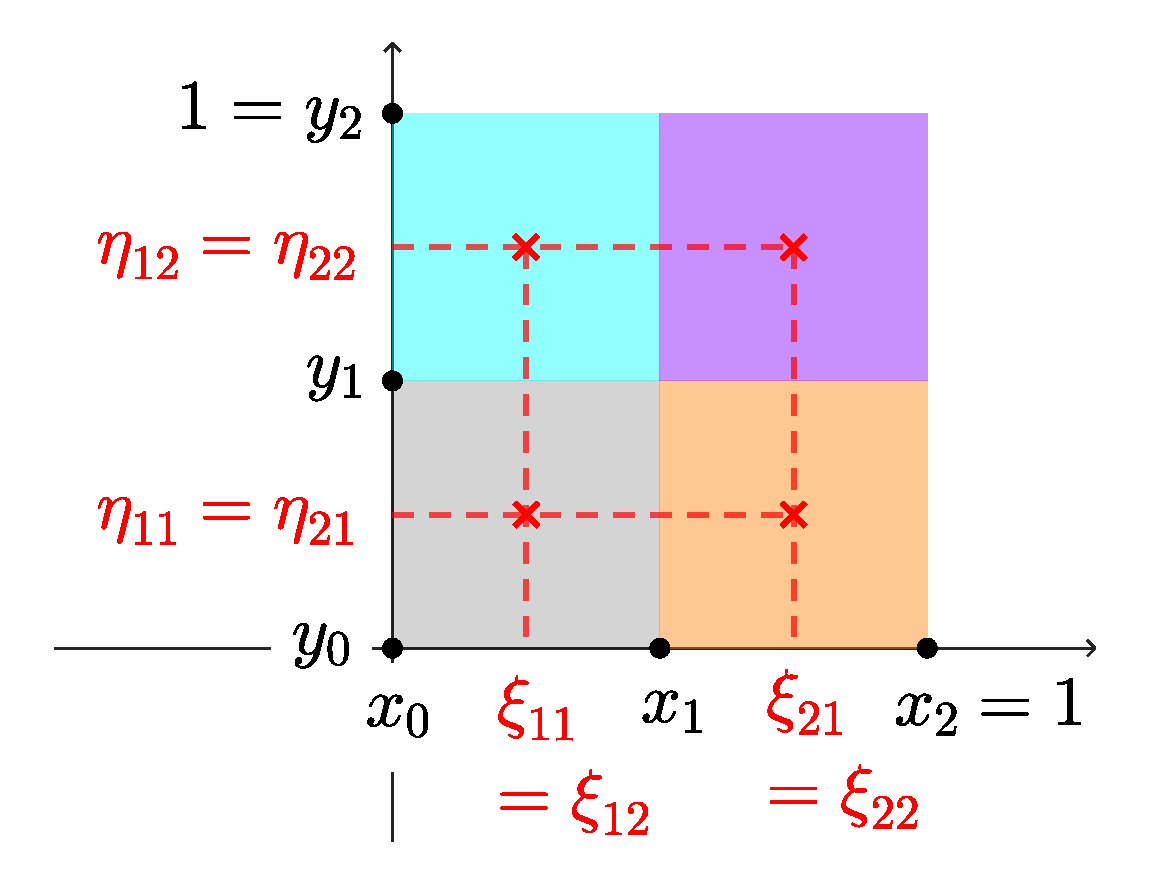
\includegraphics[height=5cm]{07/Rep3D.pdf}\\
  \end{figure}
  
  \noindent 代表点たちの具体的な座標は以下の通りである.
  \[
    \left( \xi_{11}, \eta_{11}\right) = \left( \frac{1}{4},
      \frac{1}{4}\right), \quad \left( \xi_{12}, \eta_{12}\right) =
    \left( \frac{1}{4}, \frac{3}{4}\right), \quad \left(\xi_{21},
      \eta_{21}\right) = \left(\frac{3}{4}, \frac{1}{4}\right), \quad
    \left( \xi_{22}, \eta_{22}\right) = \left( \frac{3}{4},
      \frac{3}{4}\right)
  \]
  この分割 $\Delta$と代表点集合 $\Set{\left( \xi_{ij}, \eta_{ij}
    \right)}$ に関する関数 $f(x,y)$ の Riemann 和は
  \[
    \begin{aligned}
      R\left( \Delta, \Set{(\xi_{ij}, \eta_{ij})}, f\right)
      =& \sum_{i=i}^{2} \sum_{j=1}^{2} f( \xi_{ij}, \eta_{ij}) (x_{i} - x_{i-1}) (y_{j} - y_{j-1})\\[2ex]
       =& f(\xi_{11}, \eta_{11})(x_1-x_0)(y_1-y_0) + f(\xi_{12}, \eta_{12}) (x_1-x_0)(y_2-y_1)\\[1ex]
       &+ f(\xi_{21}, \eta_{21})(x_2-x_1)(y_1-y_0)+ f(\xi_{22}, \eta_{22})(x_2-x_1)(y_2-y_1)\\[2ex]
      =& f\left(\frac{1}{4}, \frac{1}{4}\right)\left(\frac{1}{2}-0\right)\left(\frac{1}{2}-0\right)
         + f\left(\frac{1}{4}, \frac{3}{4}\right)\left(\frac{1}{2}-0\right)\left(1-\frac{1}{2}\right)\\
       &+ f\left(\frac{3}{4}, \frac{1}{4}\right)\left(1-\frac{1}{2}\right)\left(\frac{1}{2}-0\right)
         + f\left(\frac{3}{4}, \frac{3}{4}\right)\left(1-\frac{1}{2}\right)\left(1-\frac{1}{2}\right)\\[1ex]
      &= \frac{1}{32} + \frac{5}{32} + \frac{5}{32} + \frac{9}{32} = \frac{5}{8}
    \end{aligned}
  \]
  である.この値は下図の4個の直方体の体積の和に等しい.
  \begin{figure}[h]
    \centering
    \includegraphics[height=4.5cm]{07/boxes3D.png}                                                
  \end{figure}
  
\end{example}

\newpage

\subsection{ 2重積分の定義}

$f$ を有界な長方形 $K=[a,b] \times [c,d]$ で有界な $2$ 変数関数とする.
長方形 $K$ の分割
\[
  \Delta=\left( x_0, \ldots, x_m; \ y_0, \ldots, y_n\right)
\]
に対し,
\[
  |\Delta| := \max_{1 \leq i \leq m, \ 1 \leq j \leq n} \Set{ (x_{i}-x_{i-1}), \ (y_{j}-y_{j-1})}
\]
とする.$|\Delta| \to 0$ のとき,分割の仕方と代表点集
合 $\Set{(\xi_{ij}, \eta_{ij})}$ の取り方によらず Riemann
和$R\left( \Delta, \Set{(\xi_{ij}, \eta_{ij})}, f\right)$ が一定の値に
収束するならば,$f$ は $K$ で\textbf{(Riemann) 重積分
  可能} であるという.このとき,その極限値を以下のように表し,$f$ の $K$ 上の\textbf{$2$ 重積分}という.
\begin{equation}\label{eq:double-int}
  \iint_{K} f(x,y) \ dx dy
\end{equation}

$2$ 変数関数が重積分可能であるかどうかを調べるのは $1$ 変数関数のとき以
上に難しいが,$1$ 変数関数のときと同様に,有界な長方形 $[a,b] \times
[c,d]$ 上の連続関数は重積分可能であることが知られている.


\begin{theorem}\label{thm:double-integrable}
  有界な長方形 $K=[a,b] \times [c,d]$ 上連続な $2$ 変数関数は $K$ で重積分可能である.
\end{theorem}

$2$ 変数関数 $f$ が有界な長方形 $K=[a,b] \times [c,d]$ で連続であれ
ば,$K$ のいかなる分割 $\Delta$ と代表点集合に対しても,$|\Delta| \to
0$ でさえあれば必ず Riemann 和は一定の値に近づき,その値
が(\ref{eq:double-int})に等しいことをこの定理\ref{thm:double-integrable}は主張
している.\\



より一般の有界閉領域 $D$ に対しては,下図のように $D$ を含む長方形 $K=[a,b] \times
[c,d]$ を1つ取り,
\[
  f^{*}(x,y) =\left\{
    \begin{array}{cc}
      f(x,y) & \left( (x,y) \in D\right)\\
      0 & \left( (x,y) \not\in D\right)
    \end{array}
  \right.
\]
として,$f^{*}$ が $K$ 上重積分可能なら $f$ は $D$ 上重積分可能であるとし,
\[
  \iint_{D} f(x,y) \ dx dy = \iint_{K}f^{*}(x,y) \ dx dy
\]
によって $f$ の $D$ 上の2重積分を定義する.$D$ 上の重積分の値
は $D$ を含む長方形 $K$ の取り方によらない.
\begin{figure}[h]
  \centering
  \includegraphics[height=5cm]{07/region.pdf}
\end{figure}


\newpage

\subsection{2重積分の諸性質}

\begin{theorem}[$2$ 重積分の線形性]
  $f, g$ を有界閉領域 $D$ 上重積分可能な $2$ 変数関数とする.定
  数 $\alpha, \beta \in \mathbb{R}$ に対して以下が成り立つ.
  \[
    \iint_{D}\left( \alpha f(x,y) + \beta g(x,y)\right) dx dy 
    =\alpha \iint_{D} f(x,y) \ dx dy + \beta \iint_{D} f(x,y) \ dx dy
  \]
\end{theorem}

\begin{theorem}
  $2$ つの有界閉領域 $D_1, D_2$ の共通部分 $D_1 \cap D_2$ の面積が $0$
  のとき,$D_1 \cup D_2$ 上重積分可能な関数 $f$ に対して以下が成り立つ.
  \[
    \iint_{D_1 \cup D_2} f(x,y) \ dx dy = \iint_{D_1} f(x,y) \ dx dy + \iint_{D_2} f(x,y) \ dx dy
  \]
  \begin{table}[h]
    \centering
    \begin{tabular}{|cc|c|}\hline
      \multicolumn{2}{|c|}{$D_1 \cap D_2$ の面積 $=0$} & $D_1 \cap D_2$ の面積 $>0$\\ \hline
      \includegraphics[height=3cm]{07/disjoint.pdf}
     &\includegraphics[height=3cm]{07/tangent.pdf}
     & \includegraphics[height=3cm]{07/intersect.pdf}\\ \hline
    \end{tabular}
  \end{table}
\end{theorem}

\begin{theorem}\label{thm:additiveD}
  $2$ 変数関数 $f,g$ が有界閉領域 $D$ 上重積分可能かつ $f(x,y) \geqq g(x,y)$ なら以下が成り立つ.
  \[
    \iint_{D} f(x,y) \ dx dy \geqq \iint_{D} g(x,y) \ dx dy
  \]
  \begin{figure}[h]
    \centering
    \includegraphics[height=5cm]{07/monotonic.png}
  \end{figure}
\end{theorem}

\begin{theorem}
  有界閉領域 $D$ 上重積分可能な $2$ 変数関数 $f$ に対して以下が成り立つ.
  \[
    \left| \iint_{D} f(x,y) \ dx dy \right| \leqq \iint_{D} \left| f(x,y) \right| dx dy
  \]
\end{theorem}


\newpage

\subsection{累次積分による 2重積分の計算}

長方形上の連続関数の2重積分は累次積分によって
計算できる.

\begin{theorem}\label{thm:int-on-square}
  長方形 $[a,b] \times [c,d]$ 上の連続関数 $f$ に対して以下が成り立つ.
  \[
    \iint_{[a,b] \times [c,d]} f(x,y) \ dx dy = \int_{a}^{b} \left( \int_{c}^{d} f(x,y) \ dy \right) \ dx
    = \int_{c}^{d} \left( \int_{a}^{b} f(x,y) \ dx \right) \ dy
  \]
\end{theorem}

次節でこの定理\ref{thm:int-on-square}を拡張し,より一般的な有界閉領域上の2重積分の計算方法を与える.\\

\begin{example}
  \[
    \begin{aligned}
      \iint_{[0,1] \times [0,2]} \left( x^2+y^2\right) \ dx dy
      &= \int_{0}^{1} \left( \int_{0}^{2} (x^2+y^2) \ dy \right) \ dx
        = \int_{0}^{1} \left[ x^2y + \frac{y^3}{3} \right]_{y=0}^{y=2} \ dx\\[1ex]
      & = \int_{0}^{1} \left( 2x^2 + \frac{8}{3}\right) \ dx = \left[\frac{2}{3}x^3 + \frac{8}{3}x \right]_{0}^{1}
        =\frac{10}{3}
    \end{aligned}
  \]
  あるいは,次のようにも計算できる.
  \[
    \begin{aligned}
        \iint_{[0,1] \times [0,2]} \left( x^2+y^2\right) \ dx dy
      &= \int_{0}^{2} \left( \int_{0}^{1} (x^2+y^2) \ dx \right) \ dy
        = \int_{0}^{2} \left[ \frac{x^3}{3} + xy^2 \right]_{x=0}^{x=1} \ dy\\
      & = \int_{0}^{2} \left( \frac{1}{3} + y^2\right) \ dy
        = \left[ \frac{y}{3} + \frac{y^3}{3}\right]_{0}^{2}=\frac{10}{3}
    \end{aligned}
  \]
\end{example}

\vspace{1zh}

\begin{example}
  \[
    \begin{aligned}
      \iint_{[0,\pi]\times [0, \pi/3]} \sin(x-y) \ dx dy
      &= \int_{0}^{\pi} \left( \int_{0}^{\pi/3} \sin (x-y) \ dy \right) \ dx
        = \int_{0}^{\pi} \Big[ \cos(x-y) \Big]_{y=0}^{y=\pi/3} \ dx \\[1ex]
      &= \int_{0}^{\pi} \left( \cos\left( x - \frac{\pi}{3}\right) - \cos x\right) \ dx
        = \left[ \sin\left( x - \frac{\pi}{3}\right) - \sin x\right]_{0}^{\pi}\\[1ex]
      &= \sin \frac{2\pi}{3} - \sin\left( -\frac{\pi}{3}\right) =  \sqrt{3}
    \end{aligned}
  \]
  あるいは,次のようにも計算できる.
  \[
    \begin{aligned}
      \iint_{[0,\pi] \times [0, \pi/3]} \sin(x-y) \ dx dy
      &= \int_{0}^{\pi/3} \left( \int_{0}^{\pi} \sin(x-y) \ dx \right) \ dy
        = \int_{0}^{\pi/3} \Big[ -\cos(x-y) \Big]_{x=0}^{x=\pi} \ dy\\
      &= \int_{0}^{\pi/3}\left( -\cos\left(\pi-y\right) + \cos\left(-y\right) \right) \ dy
        =\Big[ \sin(\pi-y) + \sin y\Big]_{0}^{\pi/3}\\[1ex]
      &= \sin\frac{2\pi}{3} + \sin\frac{\pi}{3} = \sqrt{3}
    \end{aligned}
  \]
\end{example}

\newpage

\subsection{練習問題}

次の長方形上の2重積分を計算しよう.

\vspace{1zh}

\begin{enumerate}[(1)]

  \setlength{\itemsep}{2zh}
  
\item $\ds \iint_{[-1,1] \times [1.2]} \left( x^3-y^2\right) \ dx dy$

\item $\ds \iint_{[0,1] \times [-1,0]} e^{2x-3y} \ dx dy$

\item $\ds \iint_{[0,2] \times [0,1]} x e^{xy} \ dx dy$

\item $\ds \iint_{\left[0, \pi/2\right] \times [1,e]} \left( \cos x \right) \log y \ dx dy$
\end{enumerate}

\begin{figure}[b]
答え : (1) $\ds -\frac{14}{3}$ \quad (2) $\ds \frac{1-e^2-e^3+e^5}{6}$ \quad (3) $\ds e^2-3$ \quad (4) $1$
\end{figure}

\newpage

\subsection{(おまけ)Riemann 和の極限としての2重積分}

\vspace{1zh}

長方形上の2重積分の値を Riemann 和の極限として計算する例を挙げておく.\\


\begin{example}
  $\ds \iint_{[0,1] \times [0,1]} \left( x^2+y^2\right) \ dx dy$

  \vspace{1zh}
  
  正方形 $[0,1]\times [0,1]$ を $x$ 方向と $y$ 方向それぞれ $n$ 等分し
  て得られる分割を
  \[
    \Delta_n = \left( x_0, x_1, \ldots, x_n \ ; \ y_0, y_1, \ldots,
      y_n\right)
  \]
  とし,各小正方形 $[x_{i-1}, x_{i}] \times [y_{j-1}, y_{j}]$ の中心(対角線の交点)を代
  表点 $\left( \xi_{ij}, \eta_{ij}\right)$ とする.つまり,
  \[
    x_i = \frac{i}{n}, \quad y_j = \frac{j}{n}, \quad \xi_{ij} =
    \frac{x_{i-1}+x_{i}}{2}, \quad \eta_{ij}=\frac{y_{j-1}+y_{j}}{2}
  \]
  である.この分割 $\Delta_n$と代表点集合 $\Set{\left( \xi_{ij},
      \eta_{ij}\right)}$ に関する $f(x,y) =
  x^2+y^2$ の Riemann 和を $S_n$ とする.
  \[
    S_n := R \left(\Delta_n, \Set{\left( \xi_{ij}, \eta_{ij}\right)}, f \right)
    = \sum_{i=1}^{n} \sum_{j=1}^{n} f\left( \xi_{ij}, \eta_{ij}\right) (x_i-x_{i-1})(y_{j}-y_{j-1})
  \]
  $f$ は $[0,1] \times [0,1]$ で連続なので,定理\ref{thm:double-integrable} か
  らこの $S_n$ は $n \to \infty$ のとき収束し,
  \[
      \lim_{n \to \infty} S_n = \iint_{[0,1] \times [0,1]} (x^2+y^2) \ dx dy
  \]
  である.各 $x_{i}-x_{i-1}, y_{j}- y_{j-1}$ はいずれも $\ds
  \frac{1}{n}$
  であり,$\ds \xi_{ij} = \frac{2i-1}{2n}, \; \eta_{ij} =
  \frac{2j-1}{2n}$ なので
  \[
    \begin{aligned}
      S_n &= \sum_{i=1}^{n} \sum_{j=1}^{n} \left(\left(\frac{2i-1}{2n}\right)^2
            + \left(\frac{2j-1}{2n}\right)^2\right) \cdot \frac{1}{n} \cdot \frac{1}{n}
            = \frac{1}{4n^4} \left( \sum_{i=1}^{n} \sum_{j=1}^{n} (2i-1)^2
            + \sum_{j=1}^{n} \sum_{i=1}^{n} (2j-1)^2\right)\\[1ex]
          &= \frac{1}{4n^4} \cdot 2 \sum_{i=1}^{n}\sum_{j=1}^{n} (2i-1)^2 = \frac{1}{2n^4} \sum_{i=1}^{n} n (2i-1)^2
            = \frac{1}{4n^4} \sum_{i=1}^{n} \left( 4i^2-4i+1\right)\\[1ex]
          &=\frac{1}{2n^3} \left( 4 \sum_{i=1}^{n} i^2 - 4 \sum_{i=1}^{n} + \sum_{i=1}^{n}1\right)
            = \frac{1}{2n^3} \left( 4 \cdot \frac{n(n+1)(2n+1)}{6} - 4 \cdot \frac{n(n+1)}{2} + n \right)\\[1ex]
          &= \frac{1}{3}\left(1+\frac{1}{n}\right)\left(2+\frac{1}{n}\right) - \frac{1}{n}\left(1+\frac{1}{n}\right)
            + \frac{1}{2n^2} \to \frac{2}{3} \; (n \to \infty)
    \end{aligned}
  \]
  である.以上から,$\ds \iint_{[0,1] \times [0,1]} (x^2+y^2) \ dx dy = \lim_{n \to \infty} S_n = \frac{2}{3}$ である.
\end{example}

\newpage

定数関数 $f(x,y) = C$ は連続関数だが,定理\ref{thm:double-integrable}に頼ることなく直接2重積分を計算できる.\\

\begin{example}
  $\ds \iint_{[a,b]\times [c,d]}C \ dx dy$

  \vspace{1zh}

  $\Delta=(x_0, \ldots, x_m \ ;\  y_0, \ldots, y_n)$ を長方形
  $[a,b] \times [c,d]$ の分割とし,各小長方形
  $[x_{i-1}, x_{i}] \times [y_{j-1}, y_{j}]$ の代表点
  $\left( \xi_{ij}, \eta_{ij}\right)$ を任意に選ぶ.これらに関す
  る $f(x,y) =C$ の Riemann 和は
  \[
    \begin{aligned}
      R(\Delta, \Set{(\xi_{ij}, \eta_{ij})}, f)
      &= \sum_{i=1}^{m} \sum_{j=1}^{n} f(\xi_{ij}, \eta_{ij}) (x_{i}-x_{i-1})(y_{j}-y_{j-1})\\
      &= C \left( \sum_{i=1}^{m} (x_{i}-x_{i-1}) \right) \left(\sum_{j=1}^{n} (y_{j}-y_{j-1})\right)
        = C \left( x_{m} - x_{0} \right) \left( y_{n} - y_{0}\right)\\[1ex]
      &= C(b-a)(d-c)
    \end{aligned}
  \]
  である.よって,分割の仕方と代表点の選び方によらず Riemann 和は一定な
  ので,特に,$|\Delta | \to 0$ における極限値もその一定の値に等しい.
  よって,以下を得る.
  \[
    \iint_{[a,b] \times [c,d]} C \ dx dy = \lim_{|\Delta|
      \to 0} R\left(\Delta, \Set{\left(\xi_{ij}, \eta_{ij}\right)}, f\right) =
    C(b-a)(d-c)
  \]
\end{example}




\end{document}


\documentclass[10pt, uplatex, dvipdfmx]{jsarticle}
\usepackage{../mypackage}

\graphicspath{{../pictures}}

\setcounter{section}{7}

\begin{document}

\section{$2$ 重積分の計算(累次積分)}

\subsection{縦線集合・横線集合上の2重積分}

2重積分の計算は次の定理を使うのが一般的である.この定理の証明はおまけとして\ref{subsec:pf-iterated2}節で述べる.

\begin{theorem}\label{thm:iterated2}
  $f(x,y)$ を有界閉領域 $D$ 上連続な $2$ 変数関数とする.
  \begin{enumerate}[(1)]
    \setlength{\itemsep}{.1in}

  \item 実数 $a,b$ と閉区間 $[a,b]$ 上 $\varphi_1(x) \leqq
    \varphi_2(x)$ かつ連続な関数 $\varphi_1, \varphi_2$ によって $D$ が
    \[
      D=\Set{(x,y) | a \leqq x \leqq b, \, \varphi_1(x) \leqq y \leqq \varphi_2(x)}
    \]
    と表せるとき,$f(x,y)$ は $D$ 上重積分可能で以下が成り立つ.
    \[
      \iint_{D} f(x,y) \ dx dy = \int_{a}^{b} \left( \int_{\varphi_1(x)}^{\varphi_2(x)} f(x,y)\ dy\right) dx 
    \]

  \item 実数 $c,d$ と閉区間 $[c,d]$ 上 $\psi_1(y) \leqq
    \psi_2(y)$ かつ連続な関数 $\psi_1, \psi_2$ によって $D$ が
    \[
      D=\Set{(x,y) | c \leqq y \leqq d, \, \psi_1(y) \leqq x \leqq  \psi_2(y)}
    \]
    と表せるとき,$f(x,y)$ は $D$ 上重積分可能で以下が成り立つ.
    \[
      \iint_{D} f(x,y) \ dx dy = \int_{c}^{d} \left( \int_{\psi_1(y)}^{\psi_2(y)} f(x,y) \ dx \right) dy
    \]\\
  \end{enumerate}
  
\end{theorem}



定理\ref{thm:iterated2}(1)の $D$ を\textbf{縦線集合}(左下図)といい,
(2)の $D$ を\textbf{横線集合}(右下図)という.
\begin{figure}[h]
  \centering
  \begin{tabular}{c}
    \begin{minipage}{0.45\linewidth}
      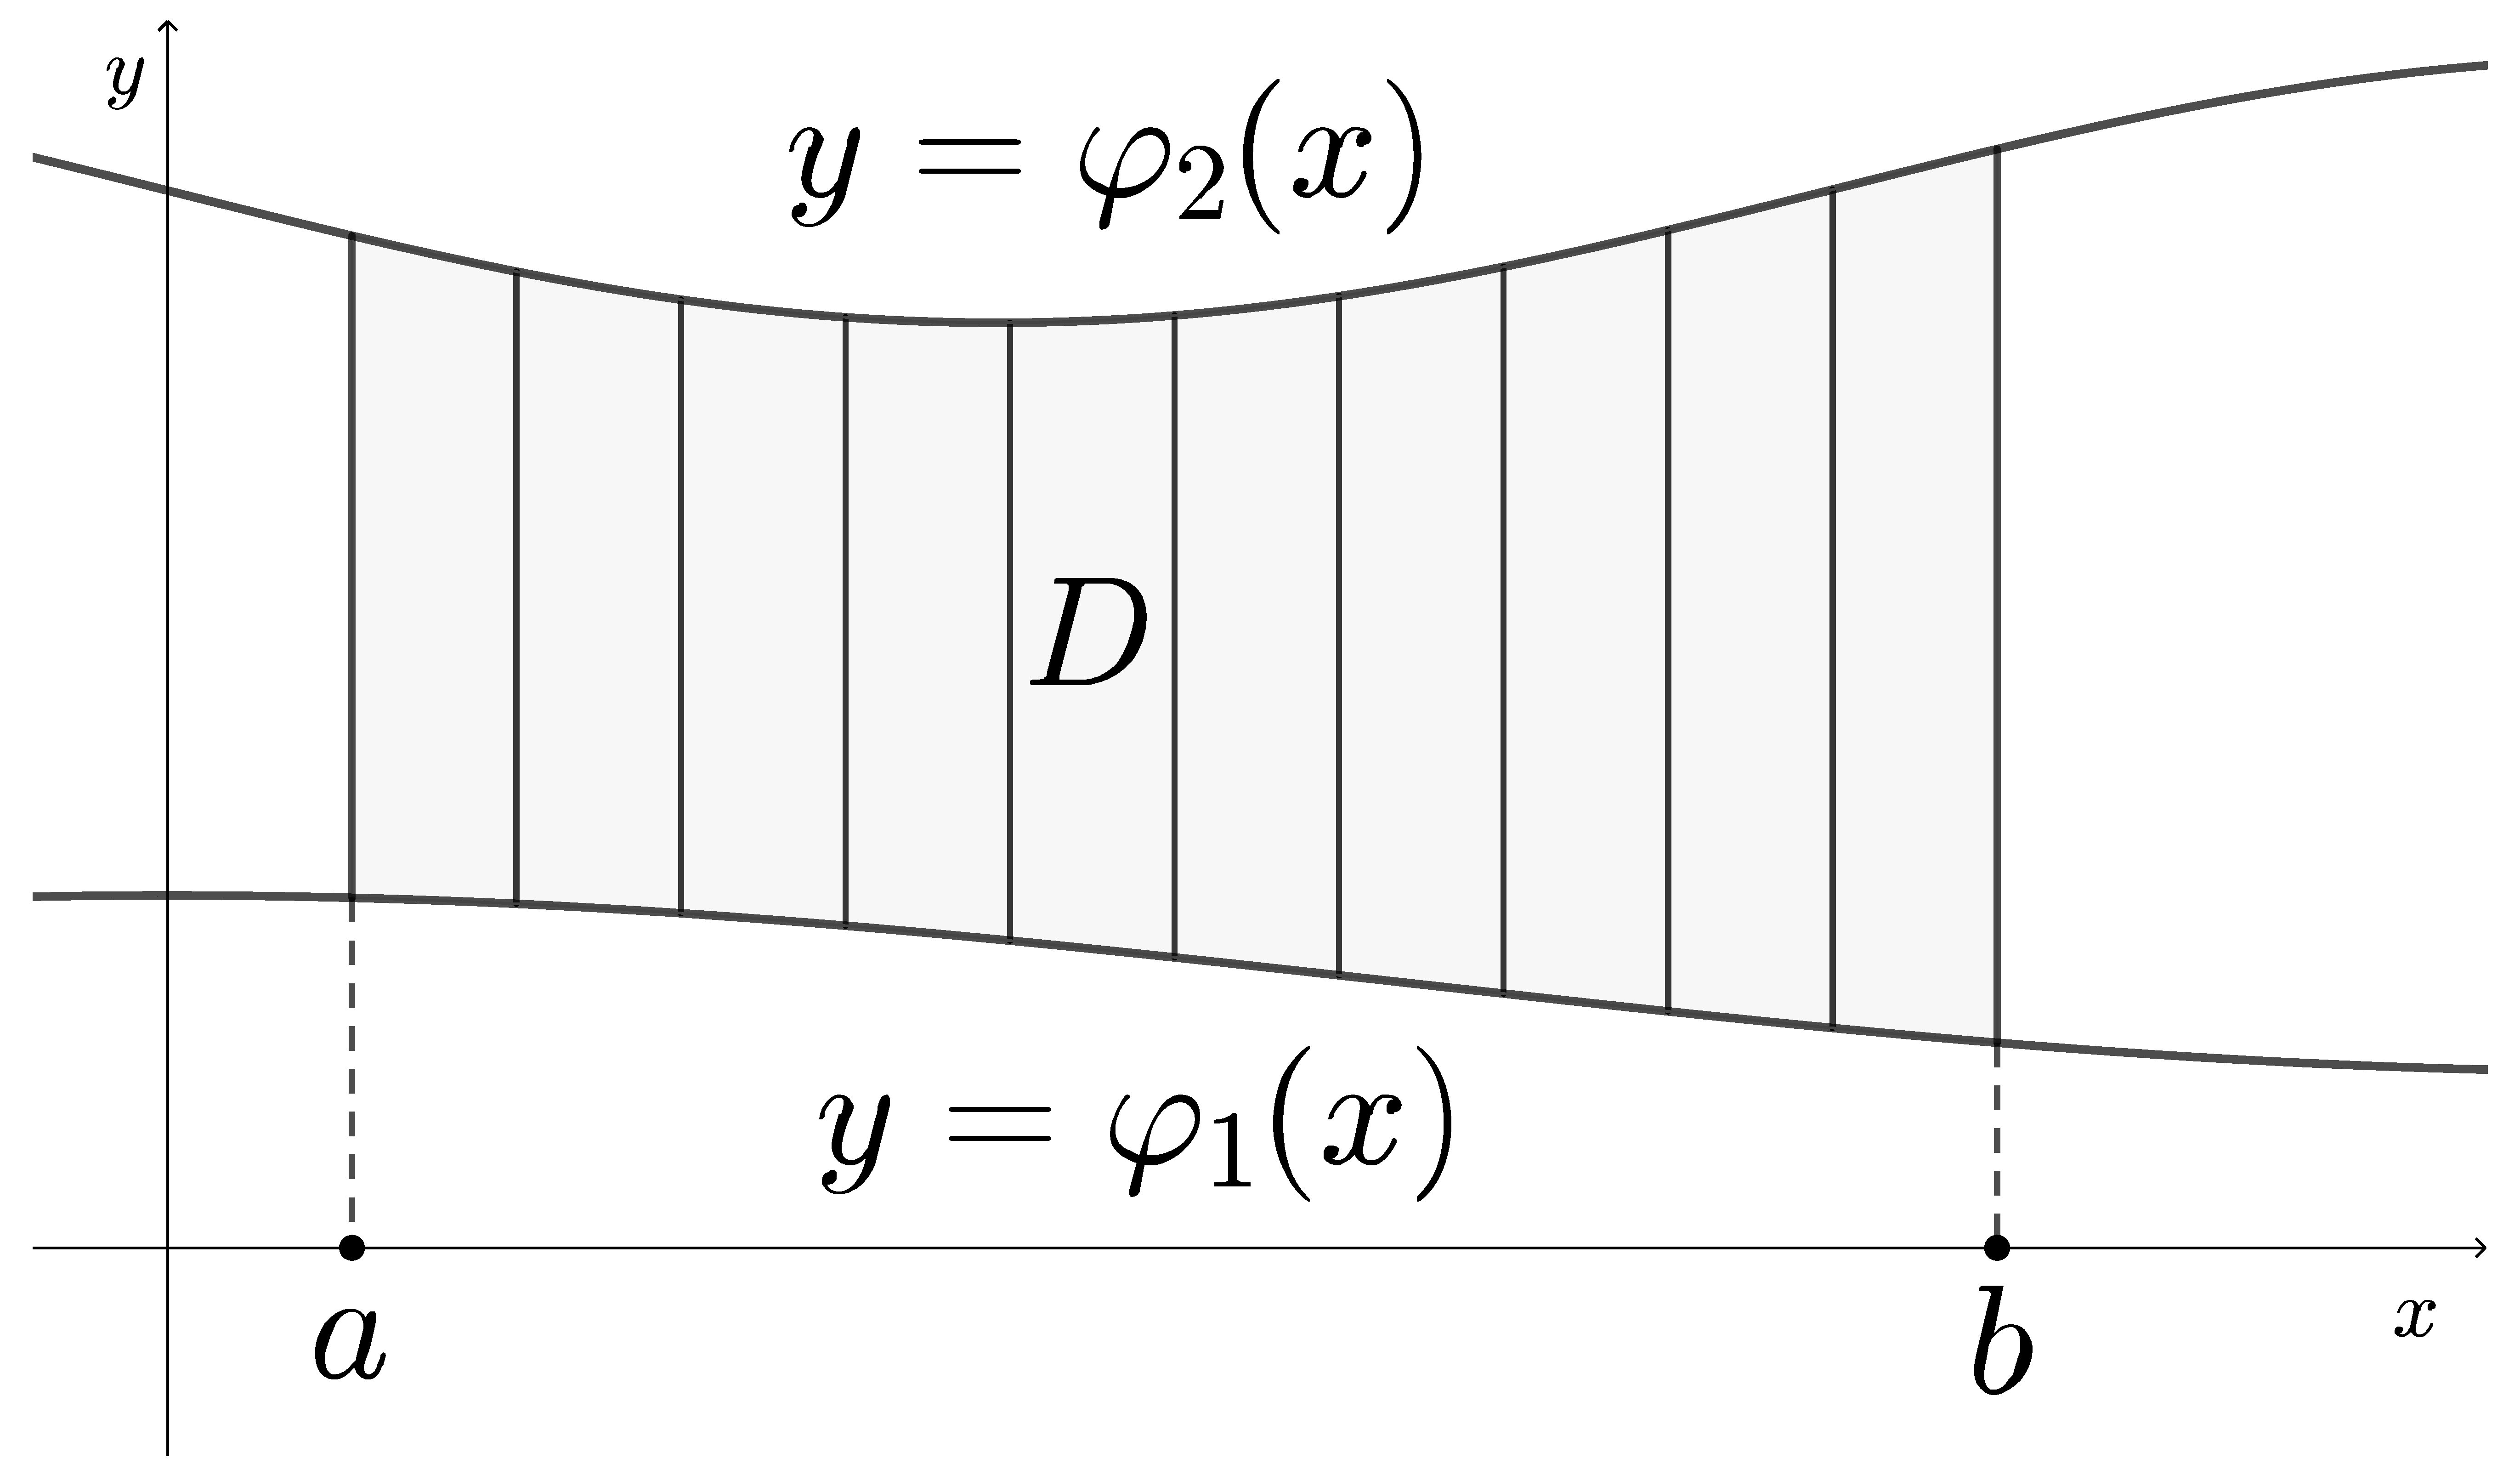
\includegraphics[height=3.5cm]{08/columnset.pdf}
    \end{minipage}
    \begin{minipage}{0.45\linewidth}
      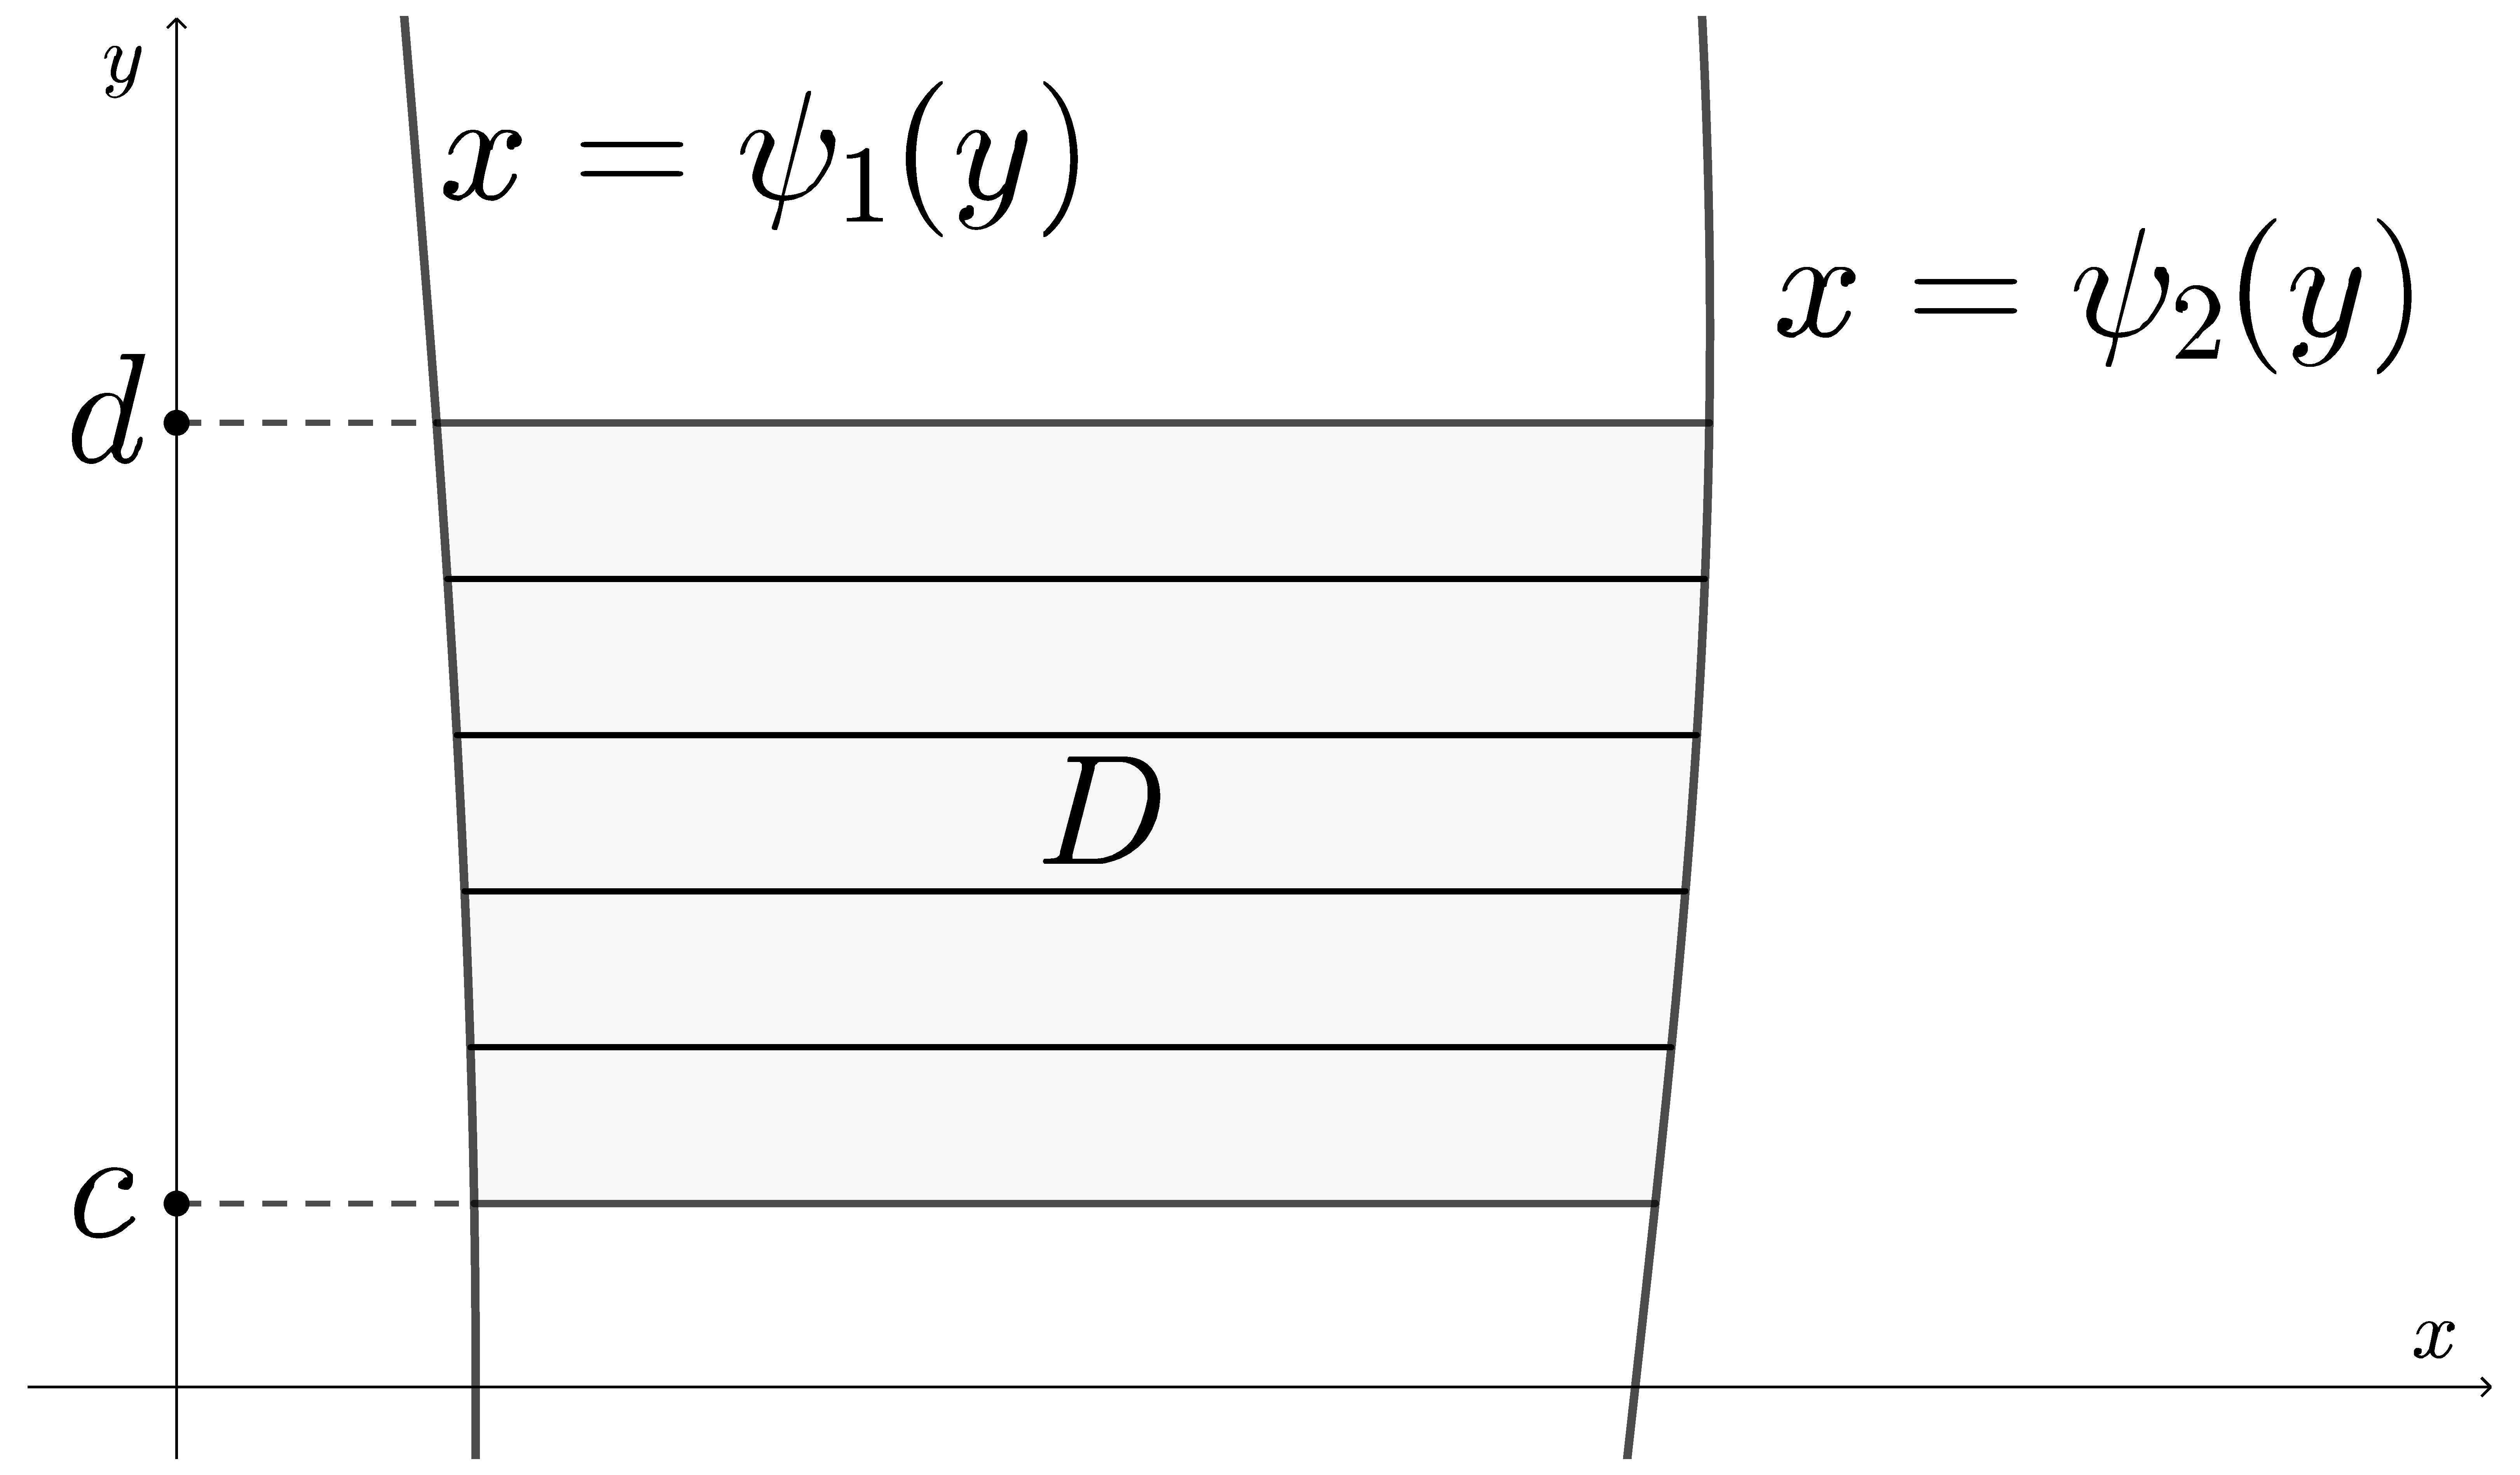
\includegraphics[height=3.5cm]{08/rowset.pdf}
    \end{minipage}
  \end{tabular}
\end{figure}

\begin{example}
  $D=\Set{(x,y) | 1 \leqq x \leqq 2, \, 0 \leqq y \leqq x}$
  に対して,$\ds \iint_{D}(x+y) \ dx dy$ は次のように計算できる.
  \begin{align*}
    \iint_{D} (x+y) \ dx dy 
    &= \int_{1}^{2} \left( \int_{0}^{x} (x+y) \ dy \right) dx
      = \int_{1}^{2} \left[ xy + \frac{1}{2}y^2 \right]_{y=0}^{y=x} dx\\
    &= \int_{1}^{2}\frac{3}{2} x^2 \ dx = \frac{1}{2}\Big[ x^3\Big]_{1}^{2} = \frac{7}{2}
  \end{align*}
\end{example}

\newpage

\subsection{定理\ref{thm:iterated2}の幾何学的意味}

$2$ 変数関数 $f(x,y)$ の有界閉領域 $D$ 上の2重積分は,$D$ の境界に
沿って伸びる $xy$ 平面に垂直な曲面と $xy$ 平面と $z=f(x,y)$ で囲まれる
立体の体積に等しい.ただし,$xy$ 平面よりも下側にある部分の体積は負の値
として扱う.定理\ref{thm:iterated2}の累次積分の内側に
\[
  F(x) = \int_{\phi_1(x}^{\phi_2(x)} f(x,y) \ dy, \quad
  G(y) = \int_{\psi_1(y)}^{\psi_2(y)} f(x,y) \ dx
\]
と名前を付ける.$F(\xi)$ の値は下図のように平面 $x=\xi$
によって立体を切ったときの断面積に等しい.同様に $G(\eta)$ の値は平
面 $y=\eta$ で立体を切ったときの断面積に等しい.従って,定
理\ref{thm:iterated2}は\textbf{立体の断面積を積分したものが体積である}こ
とを主張している.

\begin{figure}[h]
  \centering
  \includegraphics[height=11cm]{08/cutx.pdf}
\end{figure}


\newpage

\subsection{練習問題}

次の2重積分を求めよう.

\vspace{1zh}

\begin{enumerate}[(1)]

  \setlength{\itemsep}{2zh}

\item $\ds \iint_{D} \sin (x+y) \ dx dy, \quad D=\Set{(x,y) | 0 \leqq y \leqq \frac{\pi}{2}, \, 0 \leqq x \leqq y}$

\item $\ds \iint_{D} x \ dx dy, \quad D=\Set{(x,y) | y \leqq x \leqq \sqrt{y}}$
\item $\ds \iint_{D} xy \ dx  dy, \quad D=\Set{(x,y) | x+y \leqq 2, \, y^2 \leqq x, \, 0 \leqq y}$

\item $\ds \iint_{D} \sin\left( \pi x^2\right) \ dx dy, \quad D=\Set{(x,y) | y \leqq x \leqq 1, \, 0 \leqq y \leqq 1}$
  
\item $\ds \iint_{D} y \ dx dy, \quad D=\Set{(x,y) | \frac{y}{2} \leqq x \leqq 2y, \, x+y \leqq 1}$
  
\item $\ds \iint_{D} x \ dx dy, \quad D=\Set{(x,y) | -2 \leqq x \leqq 1, \, x^2+4x+1 \leqq y \leqq -x^2+2x+1}$
\end{enumerate}

\vspace{3zh}

「積分基本問題集 弍」(1) $\sim$ (4), (11), (14), (15) も参考にしてください.
\begin{center}
  \url{https://github.com/kazutsumi/Integral2/blob/main/integral2.pdf}
\end{center}

\begin{figure}[b]
  答え:(1) $1$ \quad (2) $\ds \frac{1}{12}$ \quad (3) $\ds \frac{3}{8}$ \quad
  (4) $\ds \frac{1}{\pi}$ \quad (5) $\ds \frac{1}{18}$ \quad (6) $\ds -\frac{1}{6}$
\end{figure}

\newpage

\subsection{(おまけ)定理\ref{thm:iterated2}の証明}\label{subsec:pf-iterated2}

定理\ref{thm:iterated2}の(1)を証明する.ただし,$f$ が $D$ 上で重積分可能
であることの証明は省略する.\\


1変数関数の積分に関する以下の定理\ref{thm:piecewise}を使う.

\begin{theorem}\label{thm:piecewise}
  有界閉区間で区分的に連続な $1$ 変数関数はこの区間で積分可能である.
\end{theorem}

有界閉区間 $[a,b]$ で定義された $1$ 変数関数
$f$が有限個の点$c_1, c_2, \ldots, c_n \in [a,b]$ を除いて連続で,
各 $c_i$における左側極限 $\ds \lim_{x \to c_i-0} f(x)$ と
右側極限$\ds \lim_{x \to c_i+0} f(x)$ が存在すると
き,$f(x)$ は $[a,b]$ で\textbf{区分的に連続}であるという.ただし,両
端 $a,b$では区間の内側からの片側極限のみ存在すればよい.すなわち,$a$
では右側極限が,$b$ では左側極限のみが存在すればよい.区分的に連続な関
数は有界である.また,連続関数は区分的に連続である.
\begin{figure}[h]
  \centering
  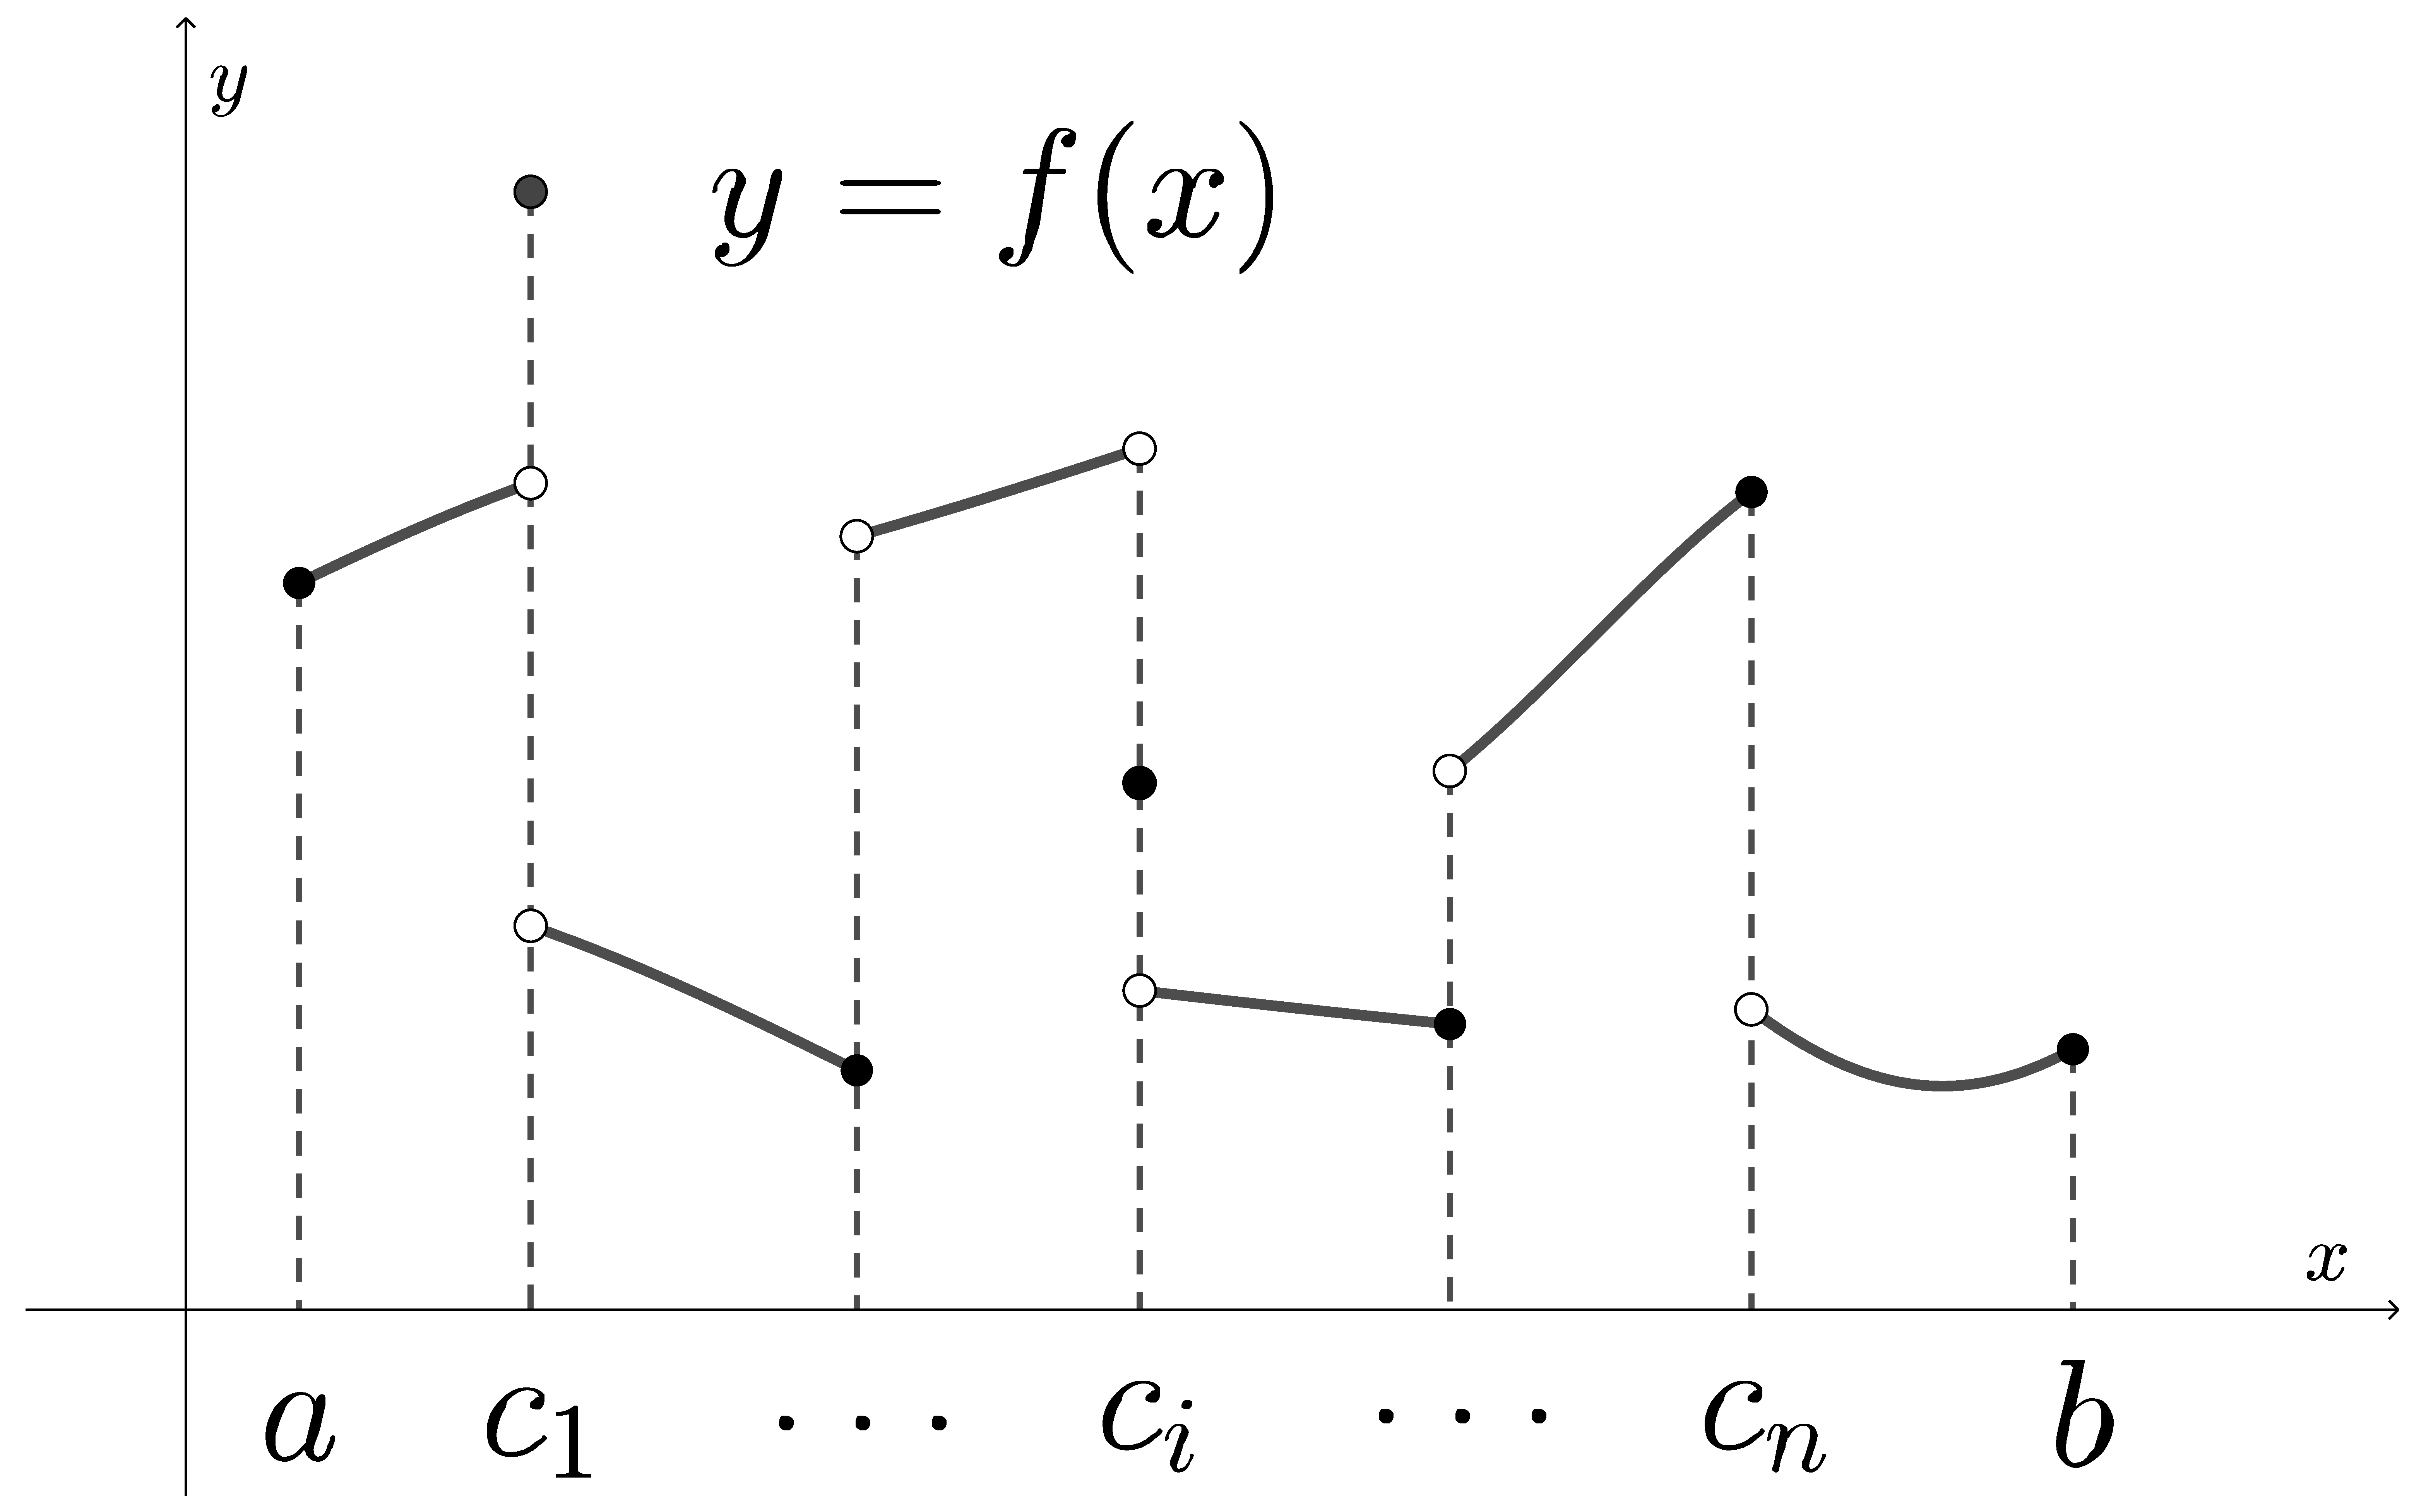
\includegraphics[height=6cm]{08/piecewise.pdf}
\end{figure}

有界閉区間 $[a,b]$ で区分的に連続な関数 $f$ の積分は,区分ごとの積分値
を足し合わせればよい.つまり,不連続な点
$c_1, c_2, \ldots, c_n \in [a,b] \; (c_1 < c_2 < \cdots <
c_n)$ と $c_0=a, \; c_{n+1}=b$ に対し
\[
  f_i(x) = \left\{
  \begin{array}{cl}
    \ds \lim_{x \to c_{i-1}+0} f(x) & (x=c_{i-1})\\
    f(x) & (c_{i-1} < x < c_{i})\\
    \ds \lim_{x \to c_{i}-0} f(x) & (x=c_{i})
  \end{array}
  \right. , \; i=,1, \ldots, n+1
\]
とすれば,各 $f_i$ は $[c_{i-1},c_{i}]$ で連続なので以下が成り立つ.
\[
  \int_{a}^{b} f(x) \ dx = \sum_{i=1}^{n+1} \int_{c_{i-1}}^{c_{i}} f_i(x) \ dx
\]


\newpage


\begin{proof}[\textbf{定理\ref{thm:iterated2}(1)の証明}]

  下図のように $D$ を含む長方形 $K=[a,b] \times [c,d]$ をとる.
    \begin{figure}[h]
    \centering
    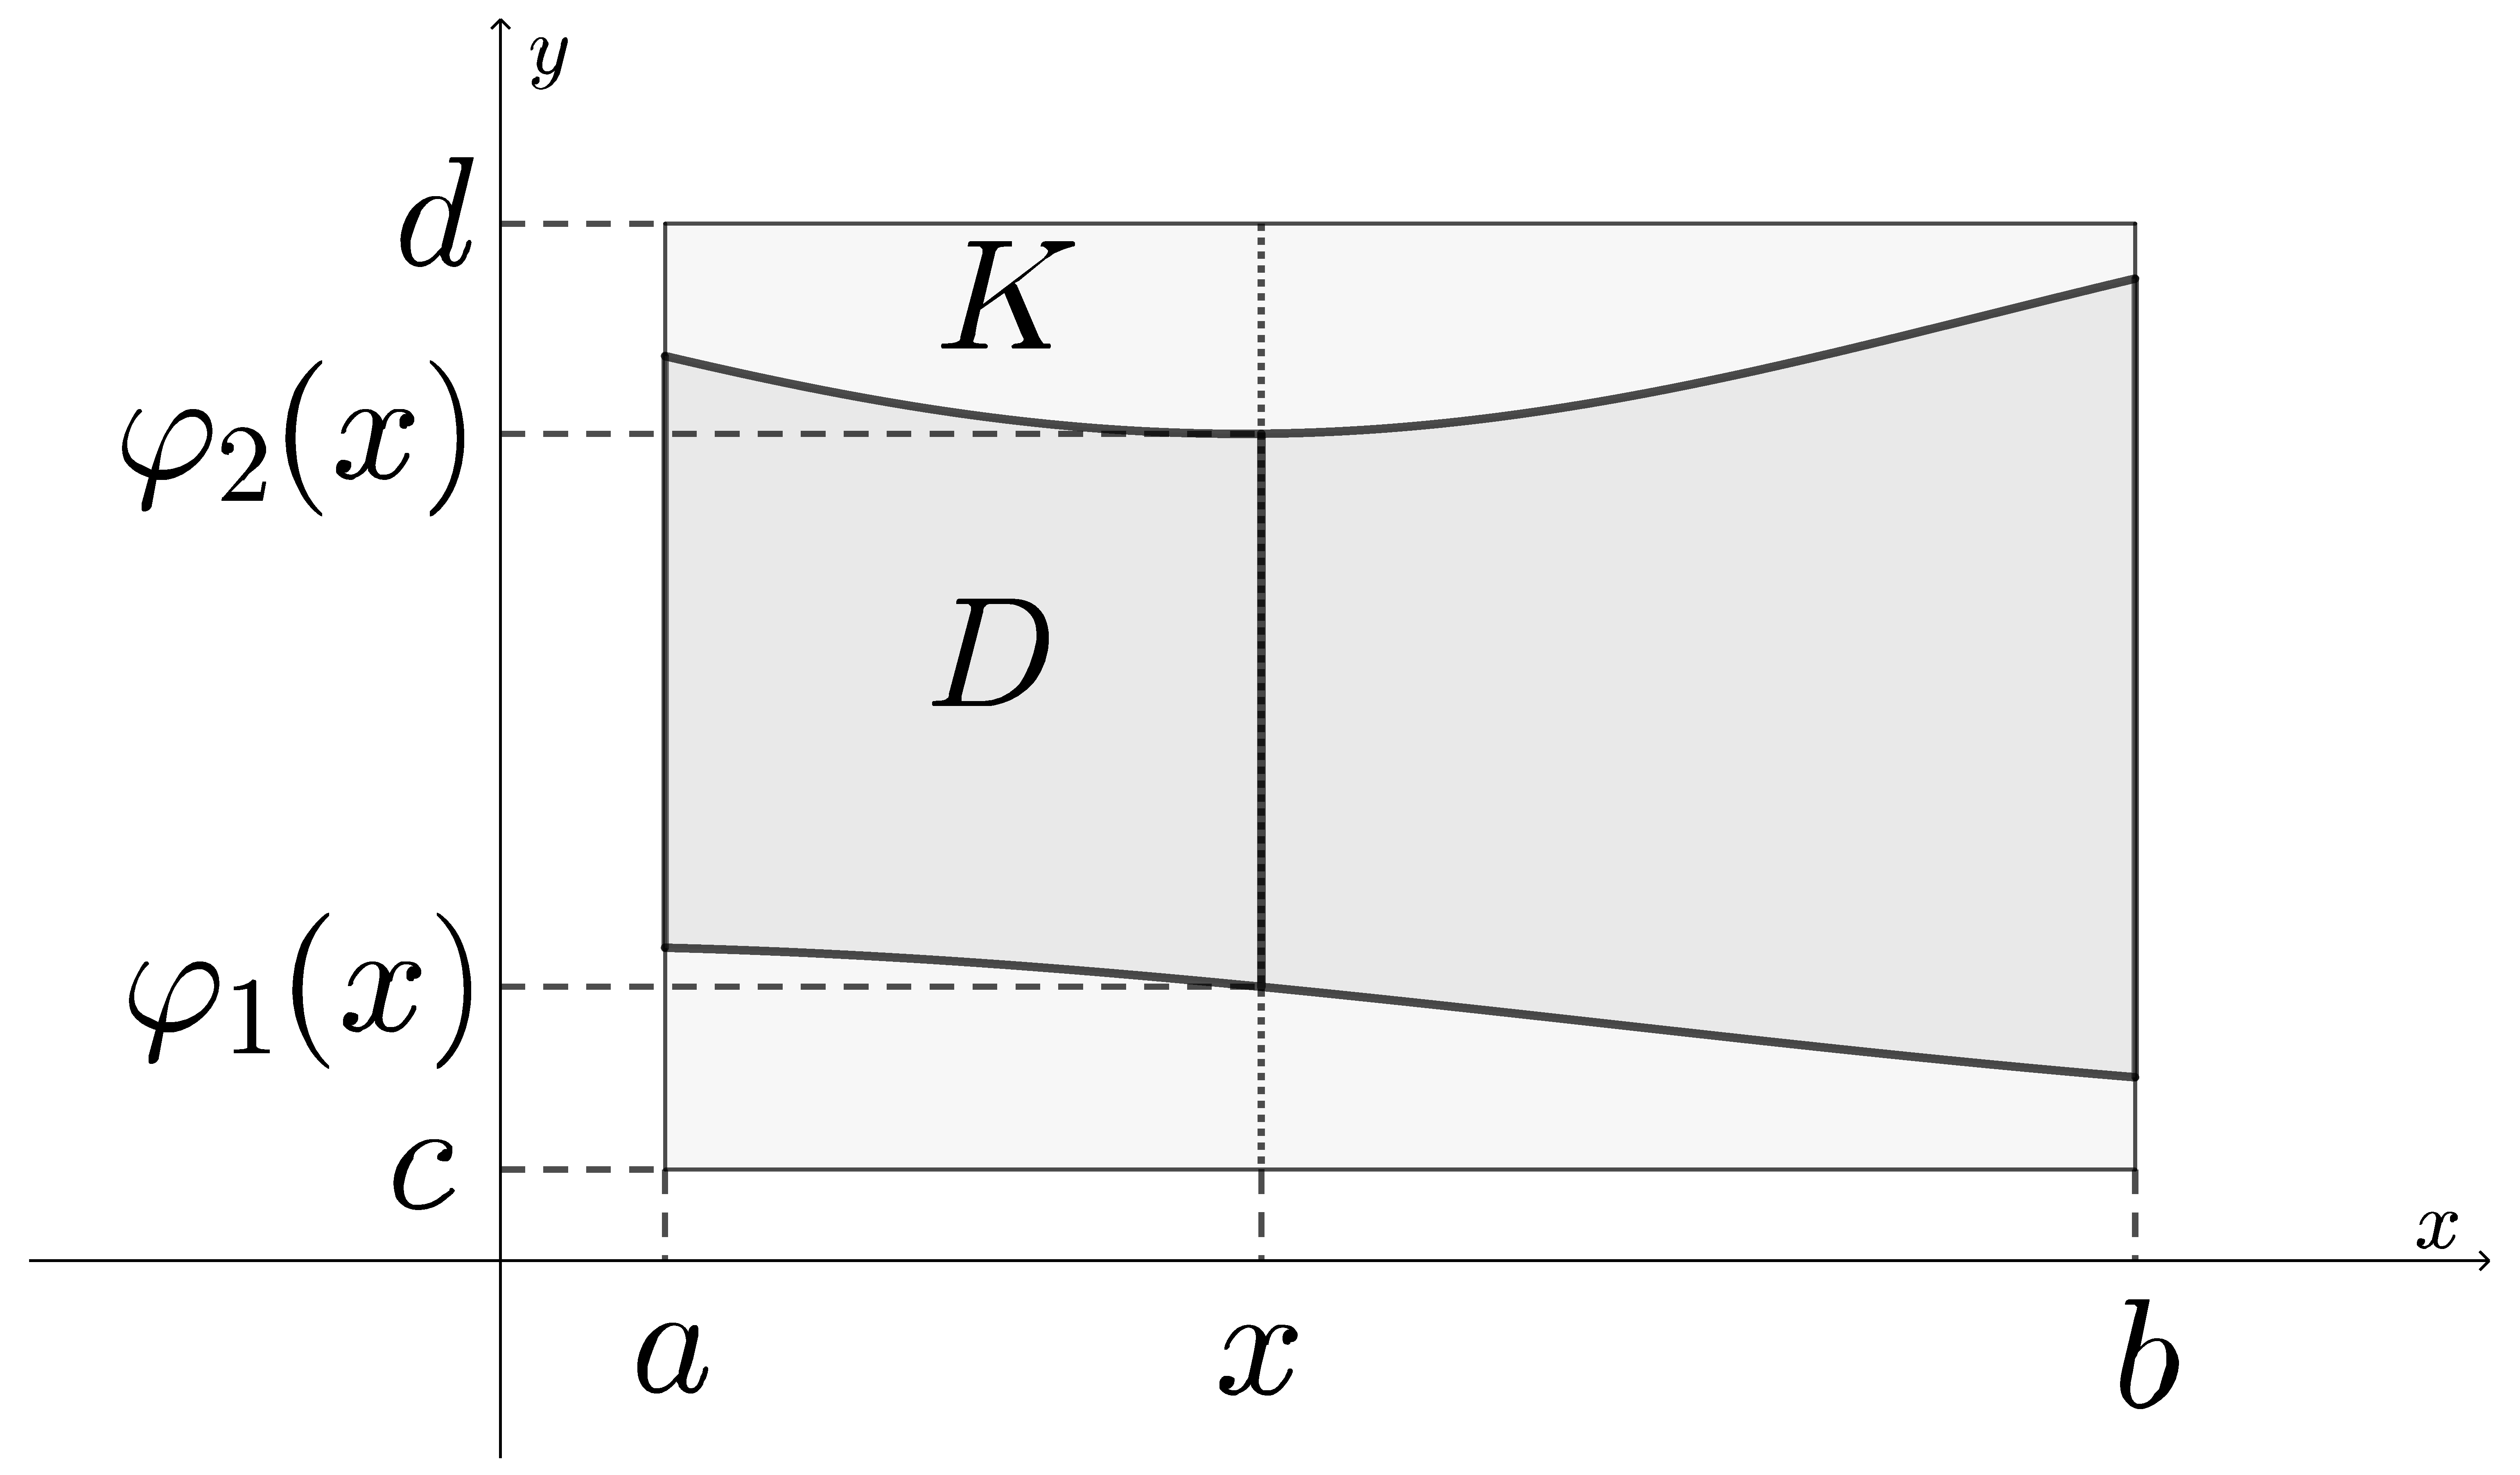
\includegraphics[height=5cm]{08/columnK.pdf}
  \end{figure}

  \noindent ここで $K$ 上の関数 $f^*$ を
  \[
    f^*(x,y) = \left\{
    \begin{array}{cl}
      f(x,y) & \left( (x,y) \in D\right)\\
      0 & \left( (x,y) \notin D \right)
    \end{array}
    \right.
  \]
  により定める.$f$ は $D$ 上重積分可能(証明略)だから,有界閉領域上
  の2重積分の定義から $f^*$ は $K$ 上重積分可能で,
  \begin{equation}\label{eq:D-K}
    \iint_{D} f(x,y) \ dx dy = \iint_{K} f^{*}(x,y) \ dx dy
  \end{equation}
  である.任意の $\xi \in [a,b]$ に対して,$y$ の $1$ 変数関
  数 $f^{*}(\xi , y)$ は $[c,d]$ において
  $\varphi_1(\xi), \varphi_2(\xi)$ を不連続点とする区分的に連続な関数であ
  る.従って,定理\ref{thm:piecewise}より $f^{*}(\xi,y)$ は$[c,d]$ で積
  分可能で,
  \begin{align*}
    \int_{c}^{d} f^{*}(\xi,y) \ dy 
    &= \int_{c}^{\varphi_1(\xi)} f^{*}(\xi, y) \ dy + \int_{\varphi_1(\xi)}^{\varphi_2(\xi)} f^{*}(\xi, y) \ dy 
      + \int_{\varphi_2(\xi)}^{d} f^{*}(\xi,y) \ dy\\
    &= 0 + \int_{\varphi_1(\xi)}^{\varphi_2(\xi)} f^{*}(\xi, y) \ dy  +0
      = \int_{\varphi_1(\xi)}^{\varphi_2(\xi)}f(\xi ,y) \ dy
  \end{align*}
  である.従って,$1$ 変数関数 $\ds F(x) = \int_{c}^{d}f^{*}(x, y) \
  dy$ が $[a,b]$ で積分可能で,かつ以下が成り立つことを証明すればよい.
  \[
    \iint_{K} f^{*}(x,y) \ dx dy = \int_{a}^{b} \left( \int_{c}^{d} f^{*}(x,y) \ dy\right) dx
  \]
  
  $\Delta=(x_0, \ldots, x_m;\ y_0, \ldots, y_n)$
  を長方形$K=[a,b] \times [c,d]$ の任意の分割とする.$x$ 方向の各小区
  間 $[x_{i-1},x_{i}]$ から代表点 $\xi_i$ を任意に選ぶ.$y$ 方向の各小
  区間 $[y_{j-1}, y_{j}]$ での $f^{*}(\xi_i, y)$ の最小値
  を $m_{ij}=f^{*}(\xi_i, s_{ij})$ とし,最大値を$M_{ij}=f^{*}(\xi_i,
  S_{ij})$ とすると,各小区間 $[y_{j-1},y_{j}]$ で
  $m_{ij} \leqq f^{*}(\xi_i, y) \leqq M_{ij}$ だから,
  \[
    m_{ij}(y_{j}-y_{j-1}) \leqq \int_{y_{j-1}}^{y_j} f^{*}(\xi_i, y) \ dy \leqq M_{ij} (y_{j} - y_{j-1})
  \]
  である.これが各 $i, j$ で成り立つので以下の不等式が成り立つ.
  \begin{align*}
    \sum_{i=1}^{m} \sum_{j=1}^{n} m_{ij} (x_{i}-x_{i-1})(y_{j}-y_{j-1})
    & \leqq \sum_{i=1}^{m}\left( \sum_{j=1}^{n} \int_{y_{j-1}}^{y_j}f^{*}(\xi_i,y) \ dy \right)(x_{i}-x_{i-1})\\
    & \leqq \sum_{i=1}^{m} \sum_{j=1}^{n} M_{ij} (x_{i}-x_{i-1})(y_{j}-y_{j-1})
  \end{align*}
  この不等式の左辺は$\Delta$ と $\Set{\left(\xi_i, s_{ij}\right)}$ に関
  する $f^{*}$ の Riemann 和であり,右辺
  は $\Delta$ と $\Set{\left(\xi_i, S_{ij} \right)}$ に関する $f^{*}$
  の Riemann 和である.また,不等式の中辺は
  \begin{align*}
    \sum_{i=1}^{m} \left( \sum_{j=1}^{n} \int_{y_{j-1}}^{y_j} f^{*}(\xi_i, y) \ dy \right) (x_i-x_{i-1})
   & =\sum_{i=1}^{m} \left( \int_{c}^{d} f^{*}(\xi_i, y) \ dy\right) (x_{i}-x_{i-1})\\
   & = \sum_{i=1}^{m} F(\xi_i)(x_{i}-x_{i-1})
  \end{align*}
  である.これは区間 $[a,b]$ の分割 $\Delta_X=(x_0, \ldots, x_m)$ と代
  表点集合 $\Set{\xi_i}$ に関する $1$ 変数関数 $F$ の Riemann 和である.
  よって,以下の不等式が成り立つ.
  \[
    R\left( \Delta, \Set{\left(\xi_i, s_{ij}\right)}, f^{*}\right) \leqq R\left(\Delta_{X},\Set{\xi_i}, F\right)
    \leqq R\left( \Delta, \Set{\left(\xi_i, S_{ij}\right)}, f^{*}\right)
  \]
  $f^{*}$ は $K$ 上重積分可能なので,$|\Delta| \to 0$ のときこ
  の不等式の左辺と右辺,従って中辺も,(\ref{eq:D-K})に収束する.ま
  た,$|\Delta| \to 0$ のとき $|\Delta_X| \to 0$ であるか
  ら,$F$ は $[a,b]$ で積分可能であり,以下を得る.
  \[
    \begin{aligned}
    \iint_{K}f^{*}(x,y) \ dx dy 
    &= \lim_{|\Delta| \to 0} R\left( \Delta, \Set{\left(\xi_i, s_{ij}\right)}, f^{*}\right)
    = \lim_{|\Delta| \to 0} R\left( \Delta, \Set{\left(\xi_i, S_{ij}\right)}, f^{*}\right)\\
    &= \lim_{|\Delta_X| \to 0} R\left( \Delta_X, \Set{\xi_i}, F\right)\
    = \int_{a}^{b} F(x) \ dx \\
    &= \int_{a}^{b} \left( \int_{c}^{d} f^{*}(x,y) \ dy \right) dx
  \end{aligned}
\]
\end{proof}



\end{document}


\documentclass[10pt, uplatex, dvipdfmx]{jsarticle}
\usepackage{../mypackage}

\graphicspath{{../pictures}}

\setcounter{section}{8}

\begin{document}

\section{2重積分の計算(変数変換)}


偏微分可能な $2$ 変数関数 $\varphi,\psi$ による変数変換 $
\begin{cases}
  x=\varphi(u,v)\\
  y=\psi(u,v)
\end{cases}
$ に対して,$u,v$ に関する $2$ 変数関数
\[
  J(u,v) = \left|
    \begin{array}{cc}
      \frac{\partial x}{\partial u} & \frac{\partial x}{\partial v}\\[1ex]
      \frac{\partial y}{\partial u} & \frac{\partial y}{\partial v}
    \end{array}
  \right|=\frac{\partial x}{\partial u} \frac{\partial y}{\partial v}
  - \frac{\partial x}{\partial v} \frac{\partial y}{\partial u}
  \; \Big( = \varphi_{u} \psi_{v} - \varphi_{v}\psi_{u}\Big)
\]
をこの変換の Jacobian という.Jacobian は以下のように書かれることもあ
る.
\[
  \frac{D(x,y)}{D(u,v)}, \quad \frac{\partial(x,y)}{\partial(u,v)}
\]

\subsection{変数変換の公式}

\begin{theorem}\label{thm:iint-trans}
  $uv$ 平面の閉領域 $E$ から $xy$ 平面の閉領域 $D$ への1対1の変数変換
  (全単射)
  \[
    \Phi:
    \begin{cases}
      x=\varphi(u,v)\\
      y=\psi(u,v)
    \end{cases}
    \quad \left(\text{ $\varphi, \psi$ は $C^1$ 級} \right)
  \]
  の Jacobian を $J(u,v)$ とし,全ての $(u,v) \in E$ に対して $J(u,v)
  \neq 0$ とする.このとき $D$ 上積分可能な連続関数 $f(x,y)$ に対して以下が成り
  立つ.
  \begin{equation}\label{eq:iint-trans}
    \iint_{D} f(x,y) \ dx dy 
    = \iint_{E} f\left( \varphi(u,v), \psi(u,v)\right) \left| J(u,v)\right| du dv
  \end{equation}
  \begin{figure}[b]
    \centering
    \includegraphics[height=8.5cm]{09/uv2xy.pdf}
  \end{figure}
\end{theorem}




\begin{example}
  次の重積分の計算に定理\ref{thm:iint-trans}を適用してみよう.
  \[
    \iint_{D} x^2 \ dx dy,  \quad D=\Set{(x,y) | \ |x+2y| \leqq 1, \, |x-y| \leqq 1}
  \] 

  $u=x+2y, \, v=x-y$ とおく.すなわち,変数変換
  \[
    \Phi :
    \begin{cases}
      x=\frac{1}{3}u+\frac{2}{3}v\\[1ex]
      y=\frac{1}{3}u-\frac{1}{3}v
    \end{cases}
  \]
  を考える.$\Phi$ は下図のように $uv$ 平面の閉領域
  \[
    E=\Set{(u,v) | -1 \leqq u \leqq 1, \, -1 \leqq v \leqq 1}
  \]
  から $xy$ 平面の閉領域 $D$ への1対1の写像である.
  \begin{figure}[h]
    \centering
    \begin{tabular}[h]{ccc}
      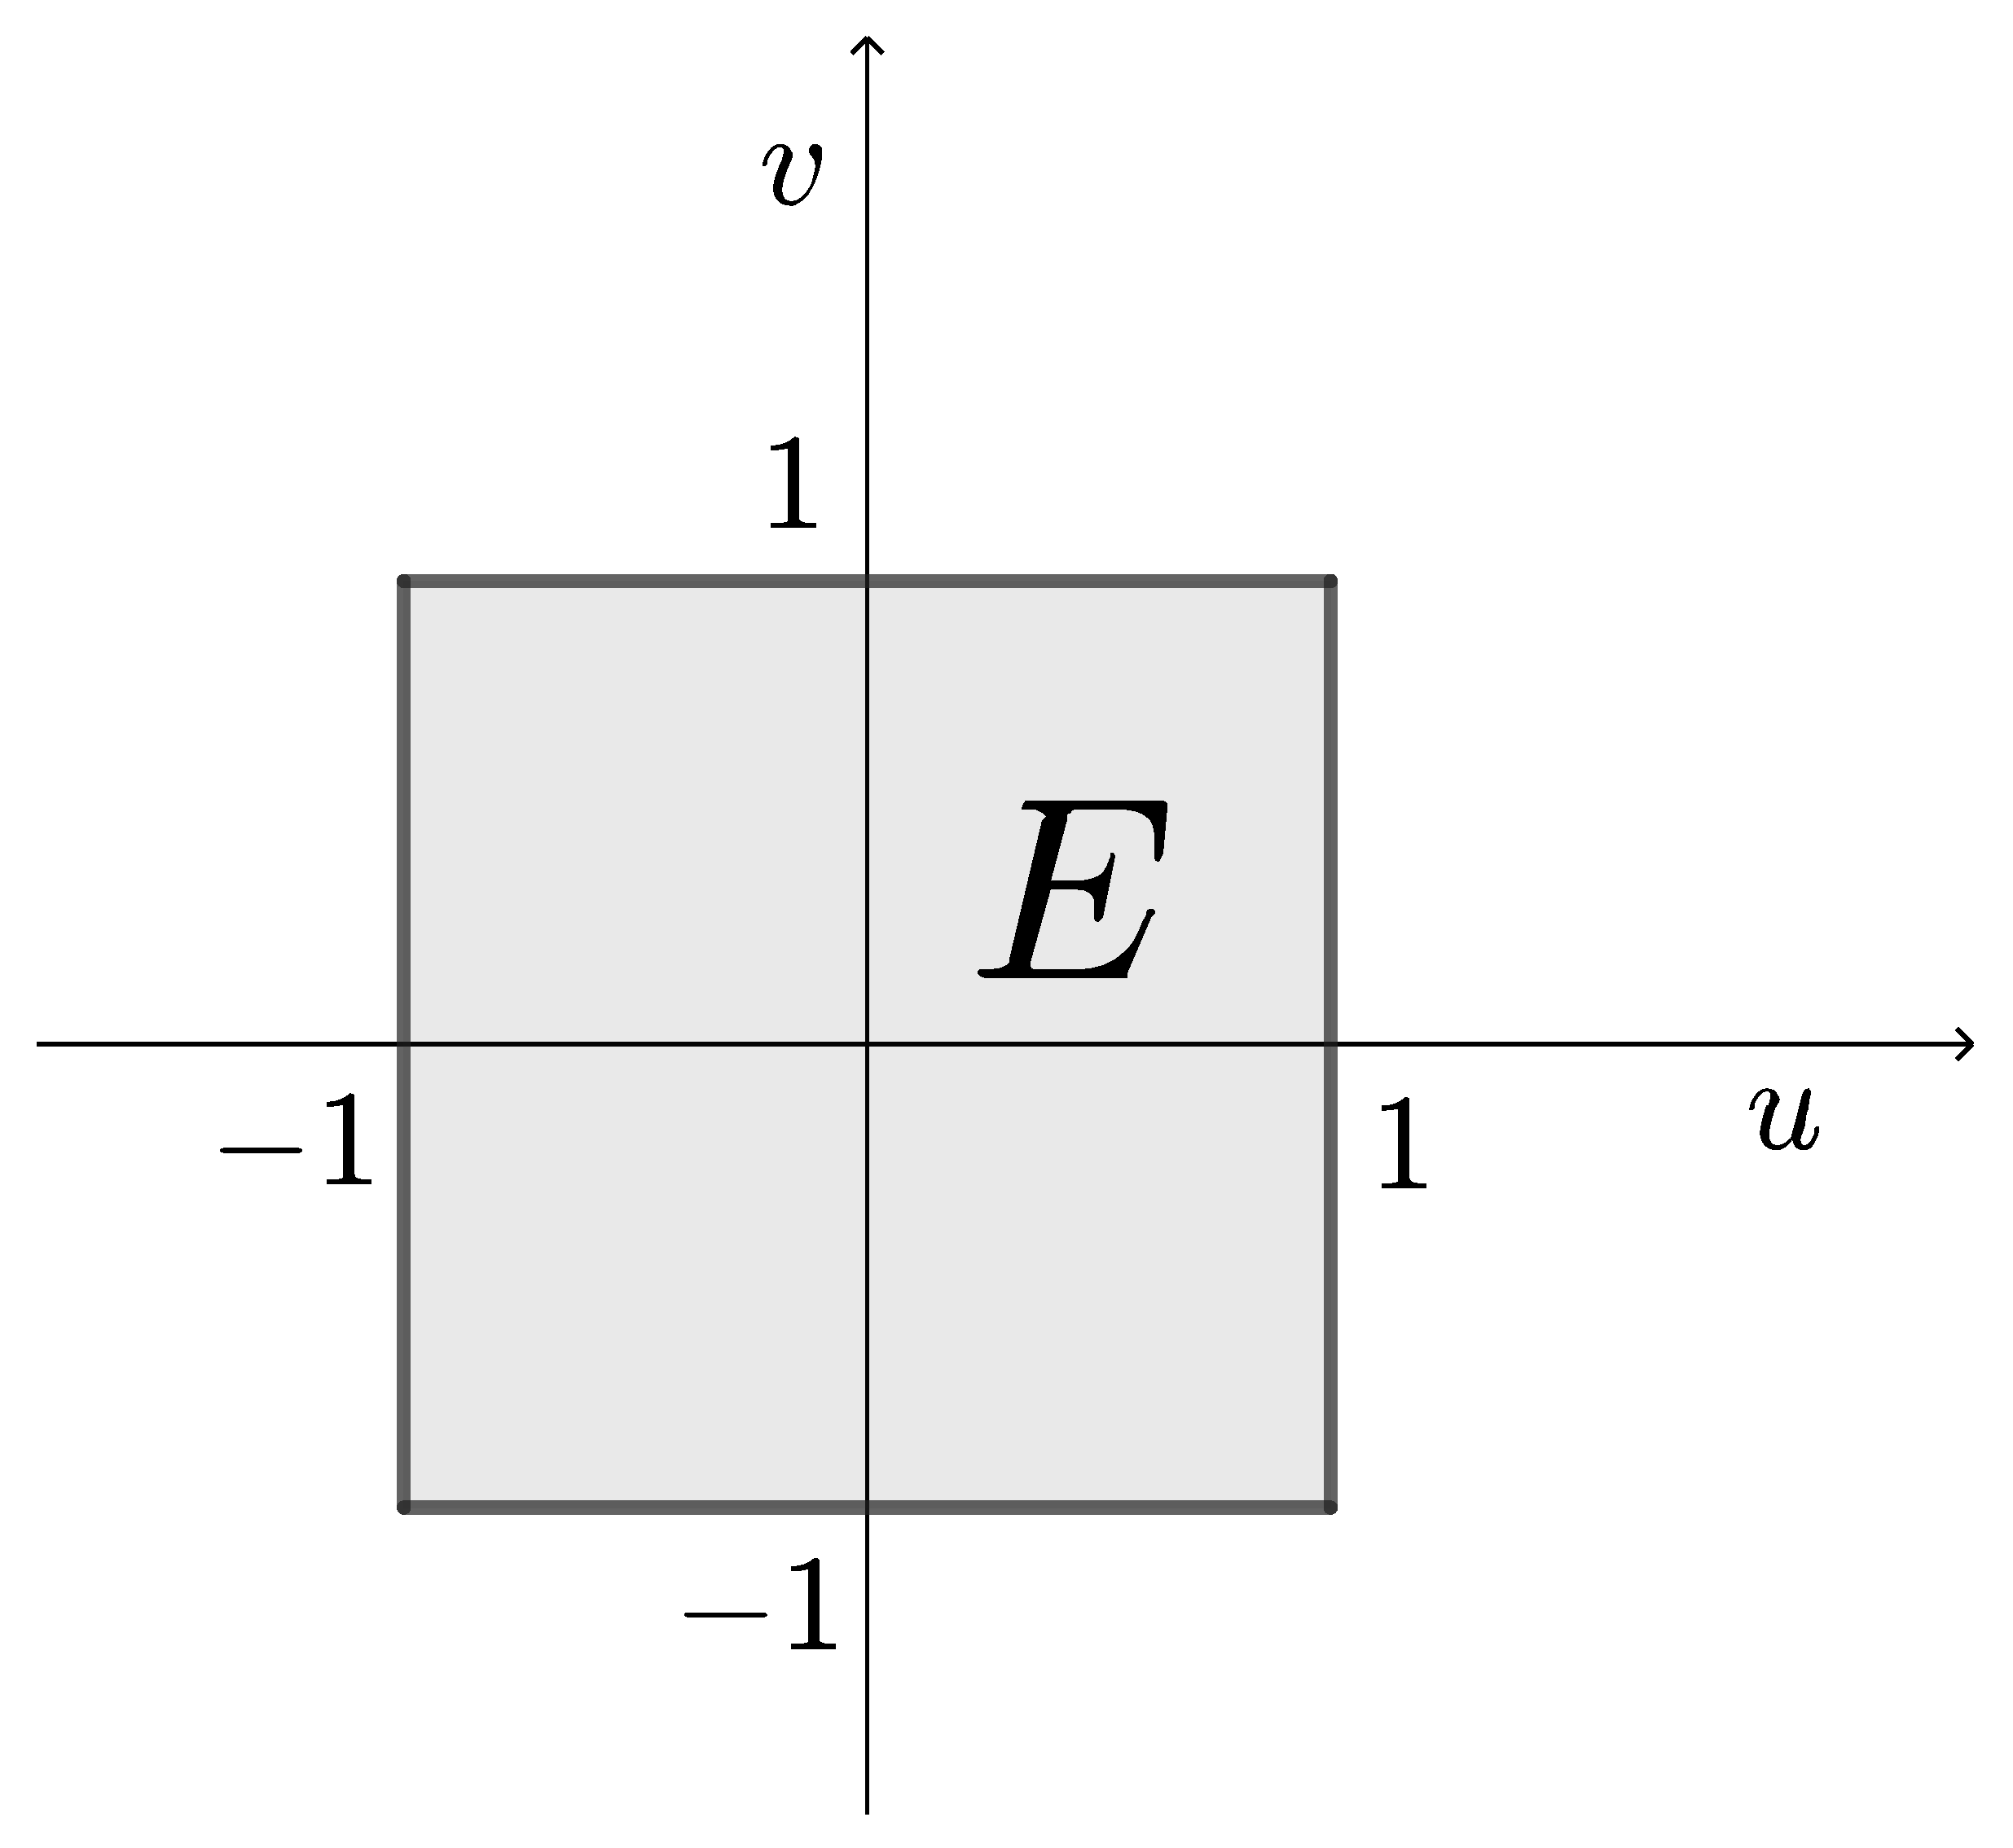
\includegraphics[height=5cm]{09/ex1uv.pdf}
      & \multirow{1}{*}[2.1cm]{$\overset{\Phi}{\longrightarrow}$}
      &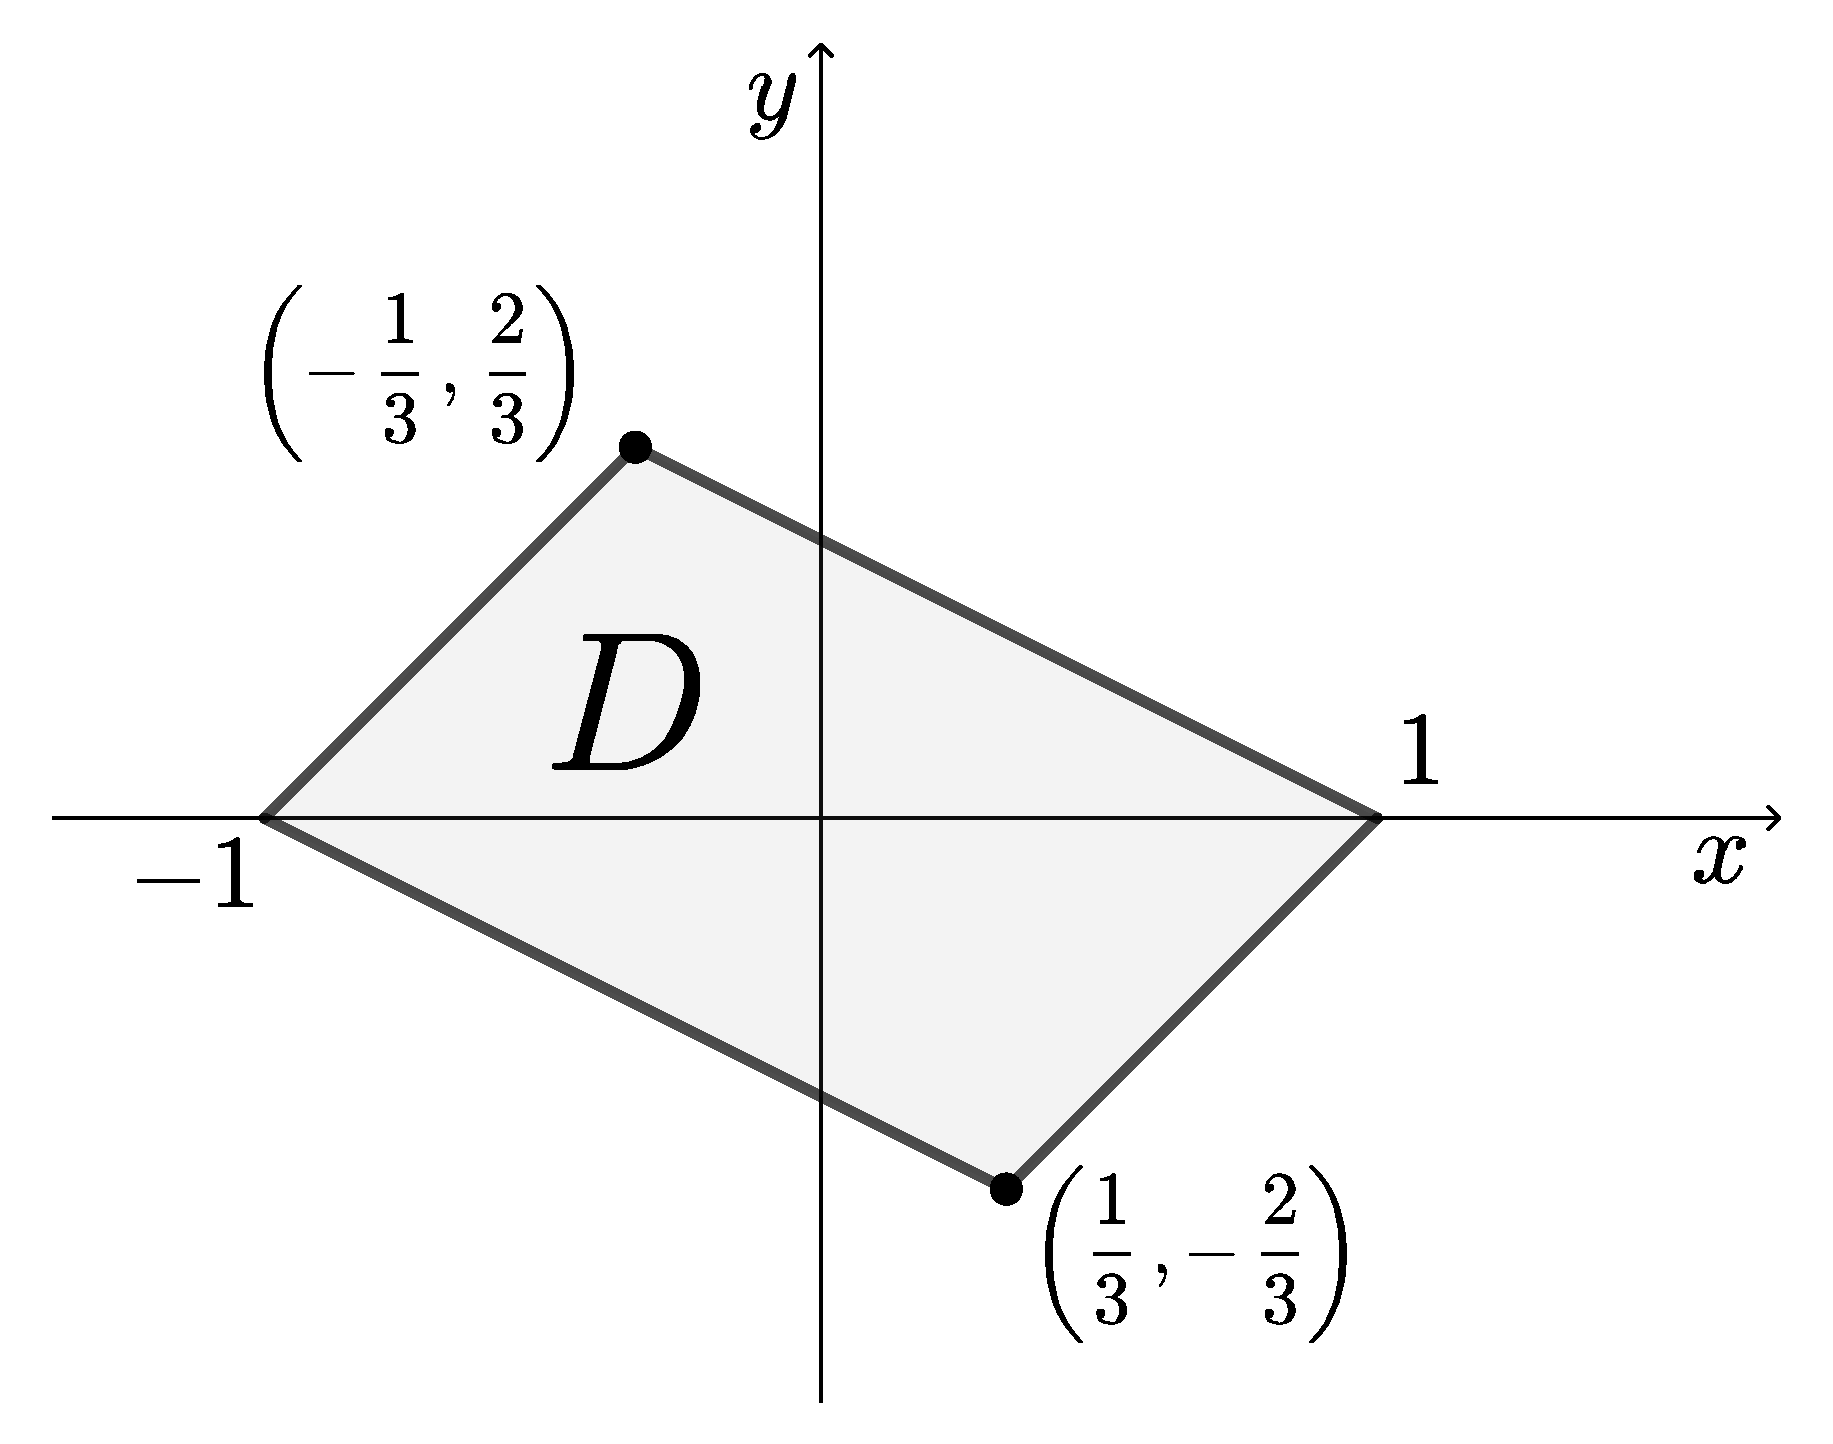
\includegraphics[height=5cm]{09/ex1xy.pdf}
    \end{tabular}
  \end{figure}

  \noindent
  変数変換 $\Phi$ の Jacobian は
  \[
    J(u,v) = \left|
      \begin{array}{cc}
        \frac{\partial x}{\partial u} & \frac{\partial x}{\partial v}\\[1ex]
        \frac{\partial y}{\partial u} & \frac{\partial y}{\partial v}
      \end{array}
    \right| =\left|
      \begin{array}{rr}
        \frac{1}{3} & \frac{2}{3}\\
        \frac{1}{3} & -\frac{1}{3}
      \end{array}
    \right| = -\frac{1}{3}
  \]
  であるから,$(u,v) \in E$ に対して $J(u,v) \neq 0$ である.よっ
  て,定理\ref{thm:iint-trans}より以下を得る.
  \begin{align*}
    \iint_{D} x^2 \ dx dy
    &= \iint_{E} \left( \frac{1}{3}u+\frac{2}{3}\right)^2 \left| J(u,v)\right| \ du dv
    =\iint_{E} \frac{1}{3}\left( \frac{1}{3}u+\frac{2}{3}\right)^2  du dv\\
    &= \frac{1}{27}\int_{-1}^{1} \left( \int_{-1}^{1} \left( u+2v\right)^2 du \right) dv
    =\frac{1}{27}\int_{-1}^{1} \left[ \frac{1}{3} \left( u+2v\right)^3 \right]_{u=-1}^{u=1} dv\\
    &=\frac{1}{81} \int_{-1}^{1} \left( \left( 2v+1\right)^3 -\left(2v-1\right)^3\right) dv
      = \frac{1}{81} \left[ \frac{(2v+1)^4}{8}- \frac{(2v-1)^4}{8}\right]_{-1}^{1}\\
    &=\frac{20}{81}
  \end{align*}

\end{example}

\newpage

\begin{remark}
  定理\ref{thm:iint-trans}の最後の等式 (\ref{eq:iint-trans}) は,変数変
  換 $\Phi$ が $E$ の面積 $0$ の部分集合 $N$ を除いて1対1で,$(u,v)
  \notin N$ に対して $J(u,v) \neq 0$ であれば成立する.
\end{remark}

例えば,正の実数 $R$ に対し極座標変換
\[
  \begin{cases}
    x = r \cos \theta\\
    y = r \sin \theta
  \end{cases}
\]
は下図のように $r\theta$ 平面の閉領域
\[
  E=\Set{ (r,\theta) | 0 \leqq r \leqq R, \, 0 \leqq \theta \leqq 2\pi}
\]
から $xy$ 平面の閉領域
\[
  D=\Set{(x,y) | x^2+y^2 \leqq R^2}
\]
への変換を与えるが,これは1対1の対応ではない.しかしながら,
\[
  N=\Set{(r, \theta) \in E | r=0} \cup \Set{(r,\theta) | \theta=2\pi}
\]
とおけば,$N$ は $E$ の面積 $0$ の部分集合であり,極座標変換は $E-N$
から $D-\Set{(0,0)}$ への1対1の対応(全単射)を与える.
\begin{figure}[h]
  \centering
  \includegraphics[height=6cm]{09/polar.pdf}
\end{figure}

\noindent
このとき,極座標変換
の Jacobian は
\[
  J(r, \theta) = \left|
    \begin{array}{cc}
      \frac{\partial x}{\partial r} & \frac{\partial x}{\partial \theta}\\[1ex]
      \frac{\partial y}{\partial r} & \frac{\partial y}{\partial \theta}
    \end{array}
  \right| = \left|
    \begin{array}{rr}
      \cos \theta & -r\sin\theta\\
      \sin \theta & r \cos \theta
    \end{array}
  \right| = r
\]
であるから,$(r, \theta) \notin N$ ならば $J(r, \theta) \neq 0$ であ
る.従って,$D$ 上重積分可能な $2$ 変数関数 $f(x,y)$ に対して,以下が成り立つ.
\[
  \iint_{D}f(x,y)\ dx dy = \iint_{E} f\left( r\cos\theta, r\sin\theta\right) r \ dr d\theta
\]

\newpage

\subsection{練習問題}


次の2重積分を求めよう.

\vspace{1zh}

\begin{enumerate}[(1)]

  \setlength{\itemsep}{2zh}
  
\item $\ds \iint_{D} (x^2-y^2)\ dx dy, \quad
  D=\Set{(x,y) | 1 \leqq x+y \leqq 2, \, 0 \leqq x-y \leqq 1}$

\item $\ds \iint_{D} e^{-x^2-y^2} dx dy, \quad
  D=\Set{(x,y) | 1 \leqq x^2+y^2 \leqq 9}$

\item $\ds \iint_{D} \sqrt{x^2+y^2}\ dx dy, \quad
  D=\Set{(x,y) | 0 \leqq y \leqq x^2+y^2 \leqq 1, \, 0 \leqq x}$

\item $\ds \iint_{D} (x^2+y^2)\ dx dy, \quad
  D=\Set{(x,y) | \frac{x^2}{4}+ \frac{y^2}{9} \leqq 1 }$

\item $\ds \iint_{D} xy\ dx dy, \quad D=\Set{(x,y) | \sqrt{x} + \sqrt{y} \leqq 1}$

\end{enumerate}


\vspace{3zh}

「積分基本問題集 弍」(5) $\sim$ (10), (12), (13) も参考にしてください.
\begin{center}
  \url{https://github.com/kazutsumi/Integral2/blob/main/integral2.pdf}
\end{center}


\begin{figure}[b]
  答え:(1) $\ds \frac{3}{8}$ \quad (2) $\ds \pi\left(e^{-1}-e^{-9}\right)$ \quad (3) $\ds \frac{\pi}{6}-\frac{2}{9}$ \quad
  (4) $\ds \frac{39\pi}{2}$ \quad (5) $\ds \frac{1}{280}$
\end{figure}




\end{document}


\documentclass[10pt, uplatex, dvipdfmx]{jsarticle}
\usepackage{../mypackage}

\graphicspath{{../pictures}}

\setcounter{section}{9}

\begin{document}

\section{広義2重積分}

有界閉領域とは限らない集合上の有界とは限らない関数の2重積分を定義する.

\subsection{増加近似列}

有界閉領域でない集合 $D$ 上の2重積分は,$D$ に近づく有界閉領域上の2重積分
の極限として定義する.そこで,まず「集合 $D$ に近づく」ということを正確
に定義する.

\begin{definition}
  $D \subset \mathbb{R}^2$ に対し,以下を満たす有界閉領域の
  列 $\Set{D_n}$ を $D$ の\textbf{増加近似列}という.
  \begin{enumerate}[(1)]
  \item
    $D_1 \subset D_2 \subset \cdots \subset D_n \subset D_{n+1}
    \subset \cdots \subset D$
  \item 任意の有界閉領域 $K \subset D$ に対して,十分大きな自然数 $n$
    を選べば $K \subset D_n$ となる.
  \end{enumerate}  
\end{definition}

\begin{example}\label{ex:Lopen}
  自然数 $n$ に対して($D_n$ に関しては $n \geqq 2$ とする)
   \begin{align*}
     D_n = \left[ \frac{1}{n}, 1\right] \times [0,1], \quad E_n=\left[e^{-n}, 1\right] \times [0,1]
  \end{align*}
   とすると,$\Set{D_n}$ と $\Set{E_n}$ はいずれも $D=(0,1] \times [0,1]$ の増加
    近似列である.
  \begin{figure}[h]
    \centering
    \begin{tabular}{cc}
      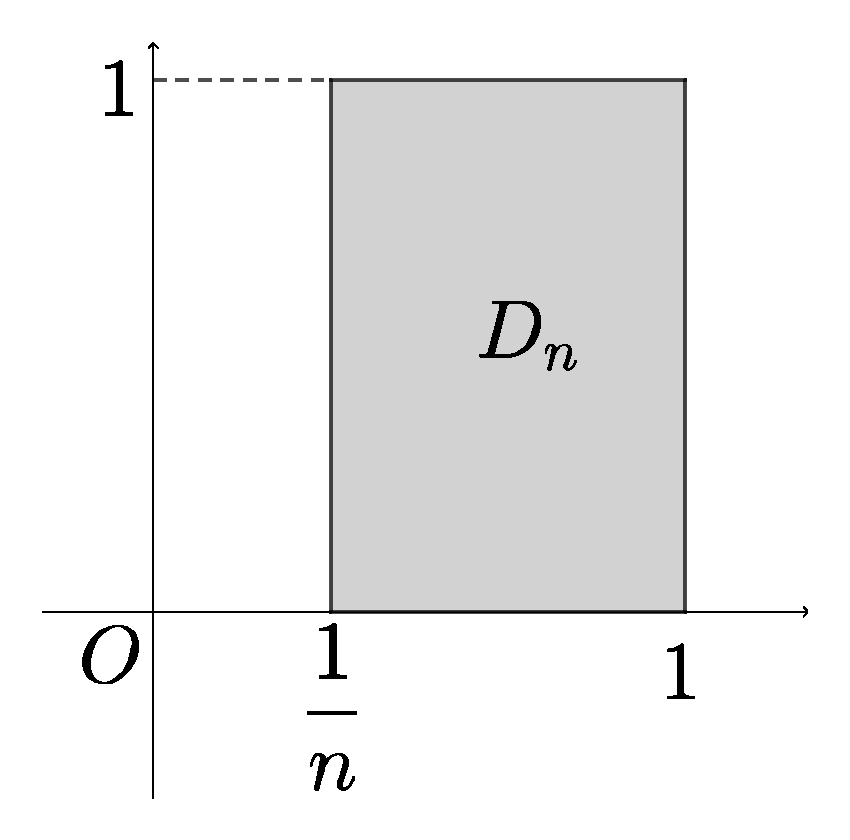
\includegraphics[height=4cm]{10/Lopen1.pdf}
      & 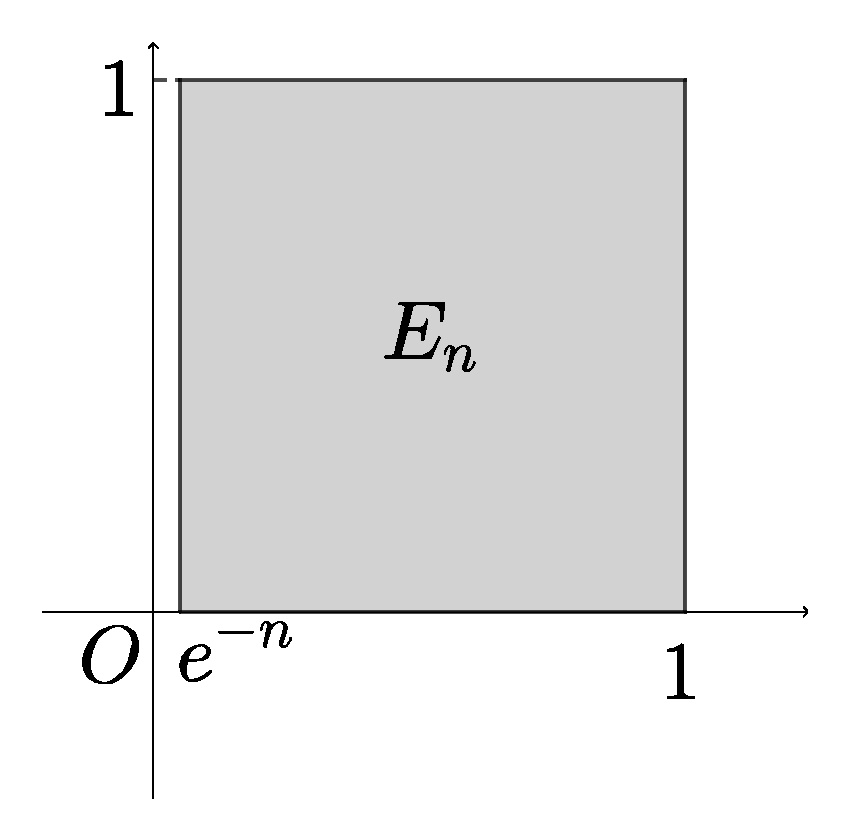
\includegraphics[height=4cm]{10/Lopen2.pdf}\\
    \end{tabular}
  \end{figure}
\end{example}

\begin{example}
  自然数 $n$ に対して
  \[
    D_n = [-n, n] \times [-n,n], \quad E_n=\Set{(x,y) | x^2+y^2 \leq n^2}
  \]
  とすると,$\Set{D_n}$ と $\Set{E_n}$ はいずれも $\mathbb{R}^2$ の増加近似列である.
  \begin{figure}[h]
    \centering
    \begin{tabular}{cc}
      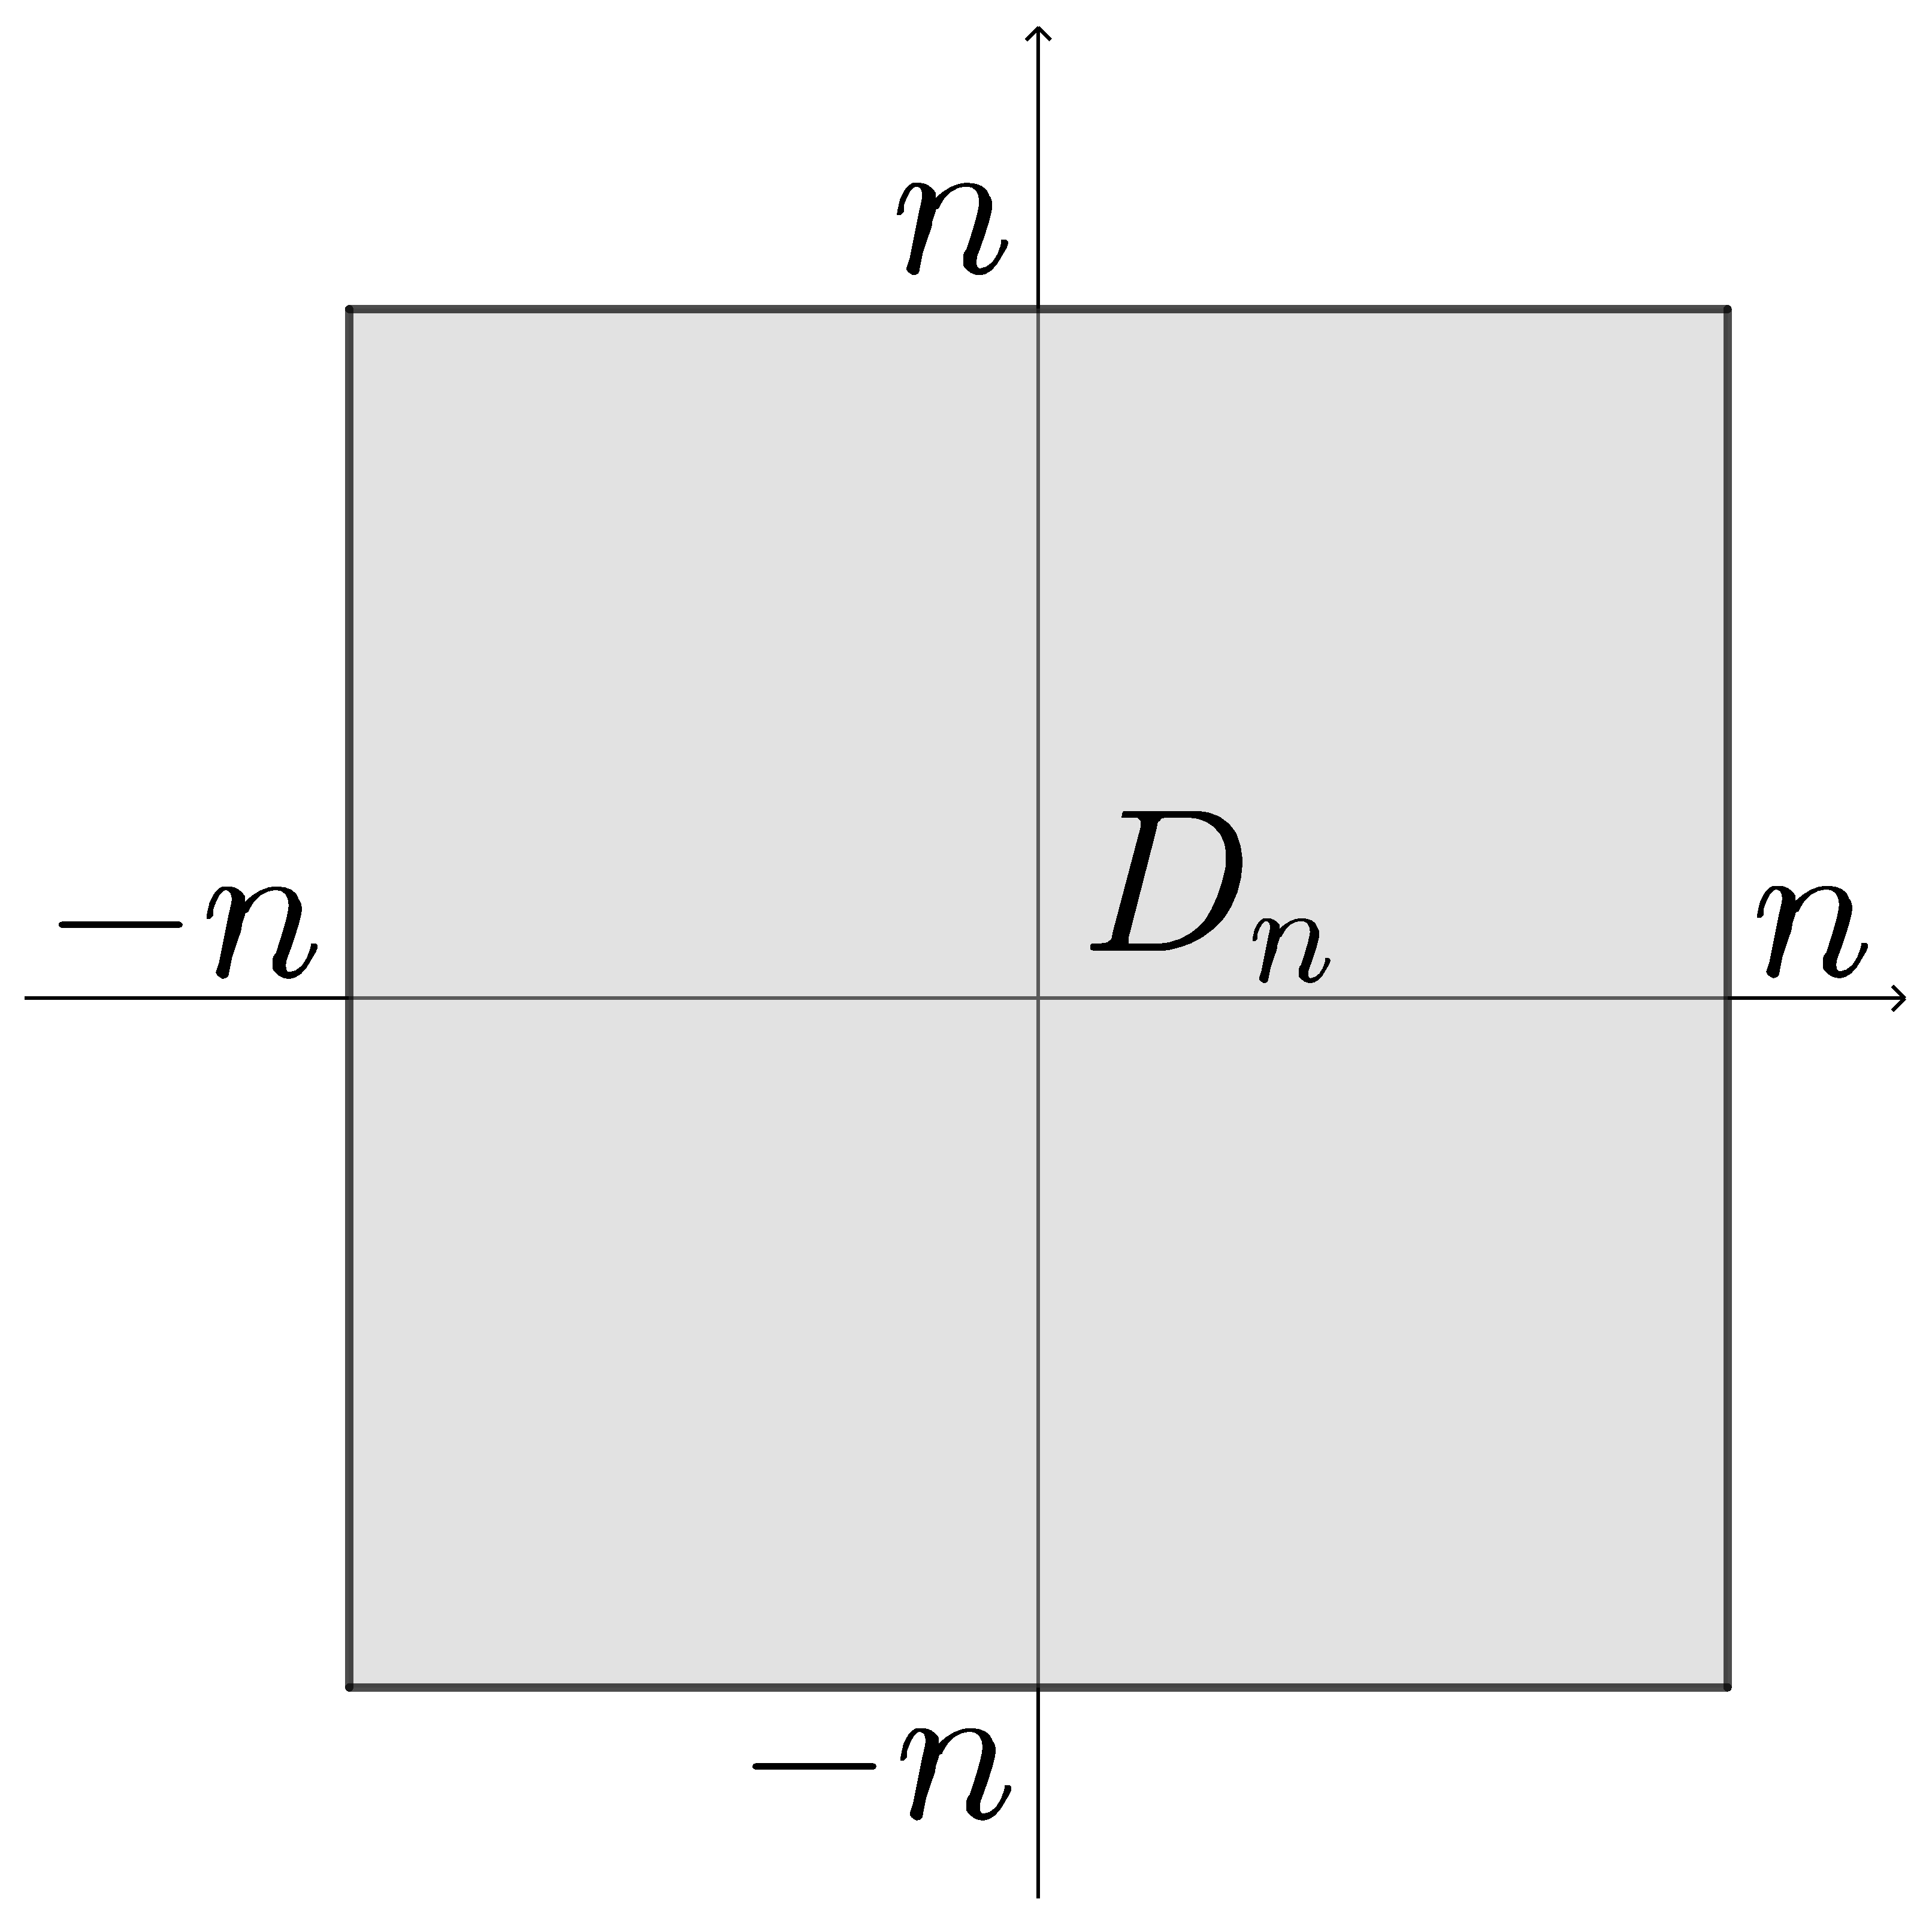
\includegraphics[height=4cm]{10/Infplane1.pdf}
      & 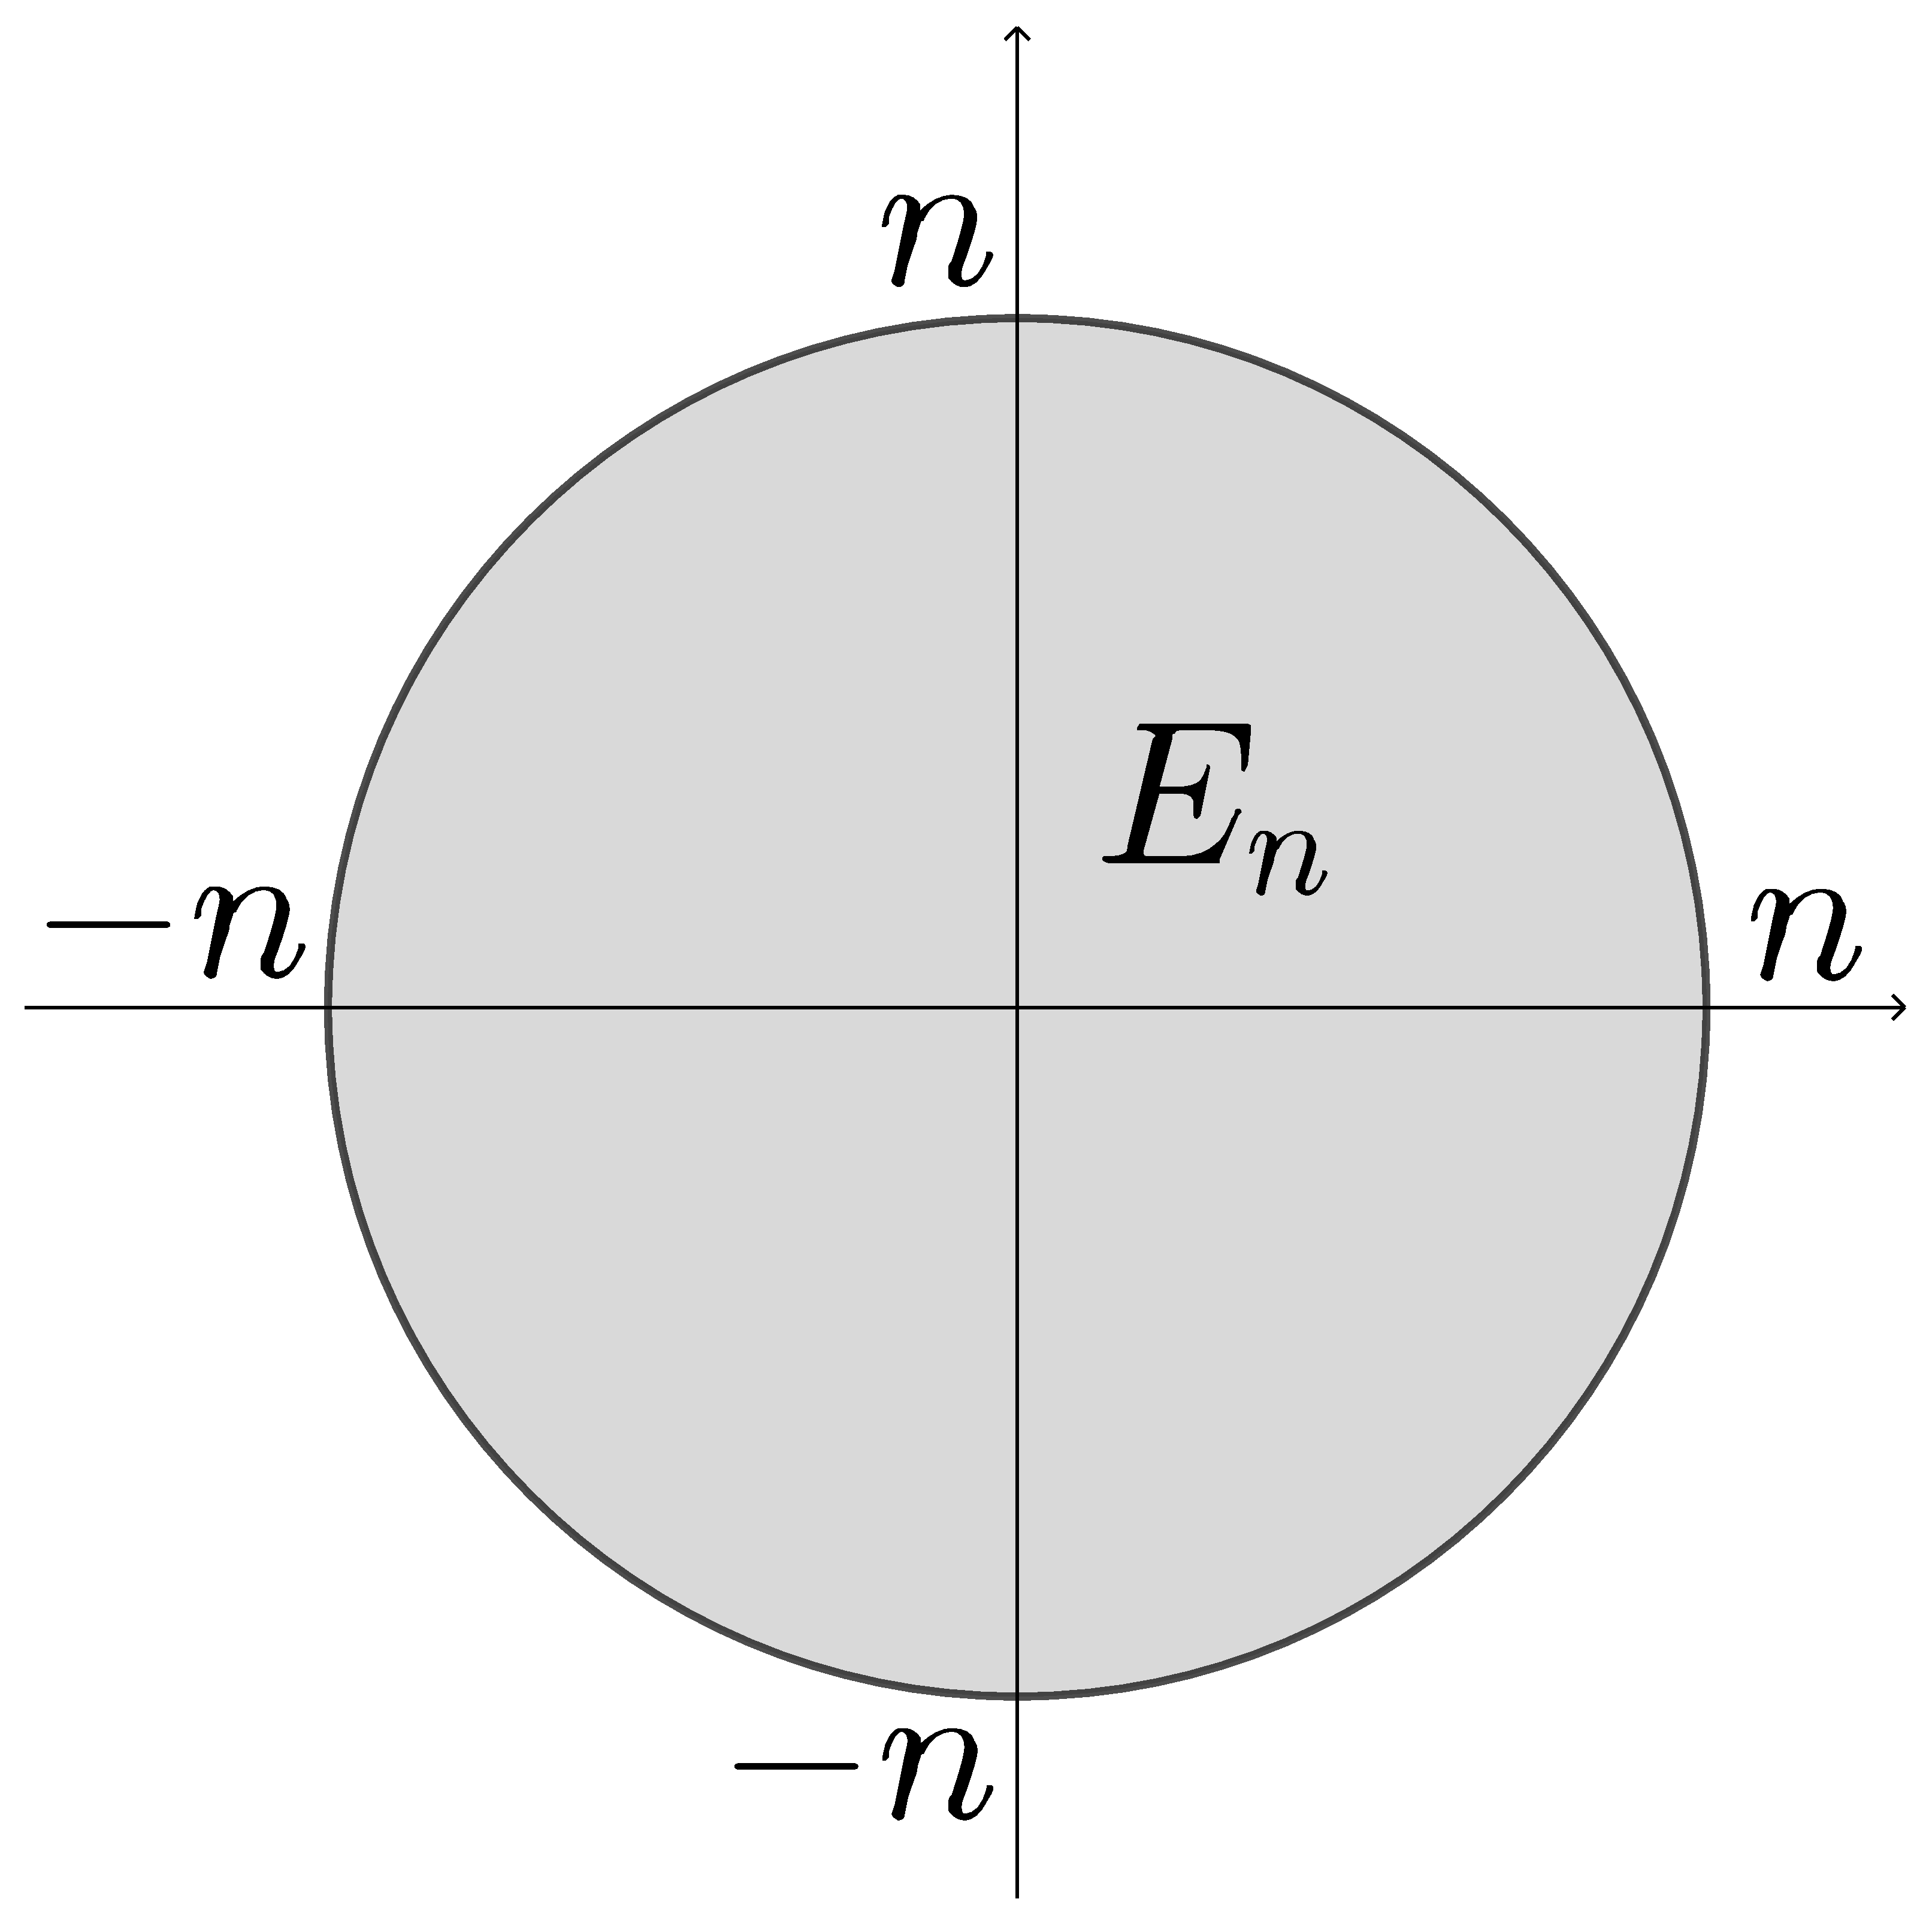
\includegraphics[height=4cm]{10/Infplane2.pdf}
    \end{tabular}
  \end{figure}
\end{example}

\subsection{広義2重積分の定義}

\begin{definition}
  $f$ を $D \subset \mathbb{R}^2$ 上定義された2変数関数とし,$D$ に含ま
  れる任意の有界閉領域上有界とする.このとき,$D$ のどんな増加近似
  列 $\Set{D_n}$ に対しても $f$ が各 $D_n$ 上重積分可能で,増加近似
  列 $\Set{D_n}$ によらず極限
  \[
    \lim_{n \to \infty} \iint_{D_n} f(x,y) \ dx dy
  \]
  が一定の値に収束するとき,$f$ は $D$
  上\textbf{広義重積分可能}であるといい,その極限値を
  \[
    \iint_{D} f(x,y)\ dxdy
  \]
  と書き,$f$ の $D$ 上の\textbf{広義2重積分}という.上の極限が存在すると
  き広義2重積分は\textbf{収束する}といい,極限が存在しなかったり増加近似列
  によって値が変わるときは\textbf{発散する}という.
\end{definition}


\begin{theorem}\label{thm:improper-conv}
  $f$ を集合 $D \subset \mathbb{R}^2$ 上の2変数関数とする.任意
  の $(x,y) \in D$ に対して $f(x,y) \geqq 0$ であるとき,$D$ のどれか1つ
  の増加近似列 $\Set{D_n}$ に対して極限
  \[
    \lim_{n \to \infty} \iint_{D_n} f(x,y)\ dx dy
  \]
  が収束するなら,$f$ の $D$ 上の広義2重積分はこの極限値に収束する.
\end{theorem}

\begin{proof}
  $\Set{E_n}$ を $D$ の任意の増加近似列とし,数列 $\Set{I_n}, \; \Set{J_n}$ を以下のように定める.
  \[
    I_n := \iint_{D_n} f(x,y) \ dx dy, \qquad J_n := \iint_{E_n} f(x,y) \ dx dy
  \]
  仮定から数列 $\Set{I_n}$ は収束するので,その極限値を $I$ とす
  る.$D$ 上で $f(x,y) \geqq 0$ なので,いずれの数列も単調増加である.
  また,増加近似列の定義から各 $E_n$ に対して十分大きな自然
  数 $N$ で $E_n \subset D_N$ となるので $J_n \leqq I_N \leqq
  I$ である.従って,$\Set{J_n}$ は上に有界で単調増加なので収束し,その極限値
  を $J$ とすれば $J \leqq I$ である.$\Set{I_n}, \Set{J_n}$ の役割を入
  れ替えて,同様の議論から $I \leqq J$ が得られる.よって, $I=J$ であ
  る.
\end{proof}
\begin{remark}
  任意の $(x,y) \in D$ に対して $f(x,y) \leq 0$ であるときも上と同様の定理が成り立つ.
\end{remark}

\begin{example}
  次の広義2重積分を計算しよう.
\[
  \iint_{D}\frac{y}{\sqrt{x}}\ dx dy, \qquad D=(0,1] \times [0,1]
\]

$D$ において $\ds \frac{y}{\sqrt{x}}>0$ だから,定
理\ref{thm:improper-conv}より $D$ の1個の増加近似列について極限を
調べればよい.例\ref{ex:Lopen}で見たように,自然数 $n \geqq 2$ に対して
$D_n = \left[ \frac{1}{n}, 1 \right] \times [0,1]$ とすれ
ば $\Set{D_n}$ は $D$ の増加近似列であり,
\begin{align*}
  \iint_{D_n} \frac{y}{(x+y)^2}\ dx dy
  &= \int_{0}^{1} \left( y \int_{\frac{1}{n}}^{1}\frac{dx}{\sqrt{x}} \right) dy
    = \int_{0}^{1}y \Big[ 2\sqrt{x}\Big]_{x=\frac{1}{n}}^{x=1} dy
    =\left( 1 - \sqrt{\frac{1}{n}}\right) \int_{0}^{1} 2y\ dy\\[1ex]
  &=  1 - \sqrt{\frac{1}{n}} \to 1 \; ( n \to \infty)
\end{align*}
なので,定理\ref{thm:improper-conv}から $\ds \iint_{D} \frac{y}{\sqrt{x}} \ dxdy = 1$ である.

\end{example}


\newpage


\subsection{練習問題}

\vspace{1zh}

\begin{enumerate}[(1)]
  \setlength{\itemsep}{2zh}

\item $\ds \iint_{D} \frac{dx dy}{\sqrt{1-x^2-y^2}}, \quad D=\Set{(x,y) \ \mid \  x^2+y^2 < 1}$

\item $\ds \iint_{D} \frac{dxdy}{\sqrt{x^2+y^2}}, \quad D=\Set{(x,y) \ \mid \  0 < x \leqq 1, \, 0 \leqq y \leqq x}$

\item $\ds \iint_{D} \tan^{-1}\frac{y}{x}\ dx dy, \quad D=\Set{(x,y) \ \mid \ x^2+y^2 \leqq 2, \, 0<x, \, 0 \leqq y}$

\end{enumerate}

\vspace{3zh}

「積分基本問題集 弍」(16) $\sim$ (24) も参考にしてください.
\begin{center}
  \url{https://github.com/kazutsumi/Integral2/blob/main/integral2.pdf}
\end{center}

\begin{figure}[b]
  答え : (1) $2\pi$  \quad (2) $\ds \log\left(1+\sqrt{2}\right)$  \quad (3) $\ds \frac{\pi^2}{8}$
\end{figure}


\newpage

\subsection{(おまけ)広義2重積分の収束・発散}


  増加近似列の選び方によって極限値が異なるとき広義積分は発散すると定義した.例
  として
 \[
   D = [0,1] \times [0,1] - \{(0,0)\}
   =\Set{(x,y) \ \mid \ 0 \leqq x \leqq 1, \, 0 \leqq y \leqq 1, \, (x,y) \neq (0,0)} 
 \]
 に対し,以下の広義2重積分を考えてみる.
 \[
   \iint_{D} \frac{x-y}{(x+y)^3}\ dx dy
 \]
 $D_n, E_n \; (n \geqq 2) $ を下図のような閉領域と
 すると, $\Set{D_n}$ と $\Set{E_n}$ はいずれも $D$ の増加近似列である.
 \begin{figure}[h]
   \centering
   \begin{tabular}{cc}
     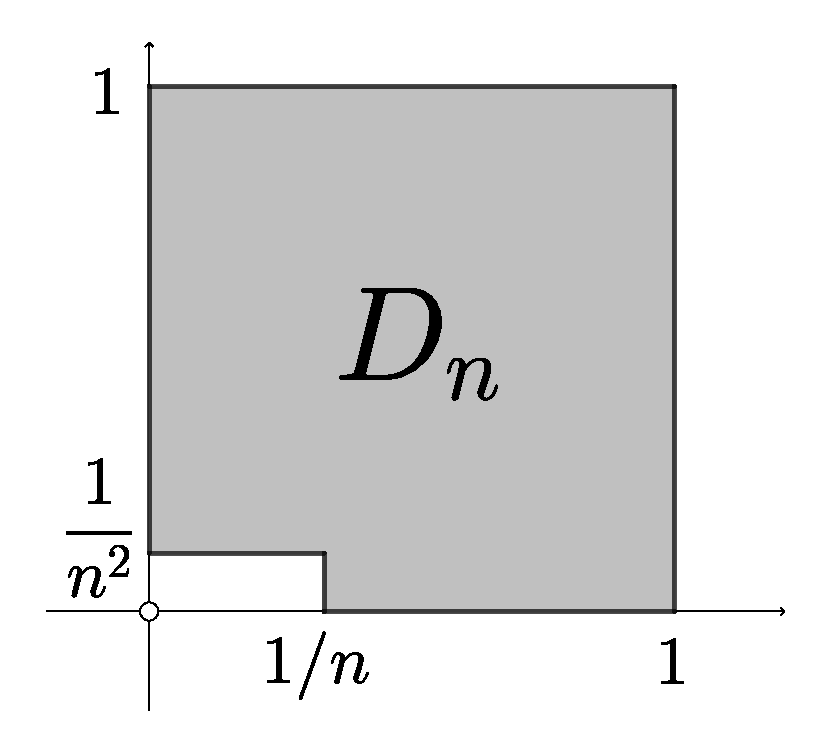
\includegraphics[width=4.8cm]{10/rowlong.pdf}&
     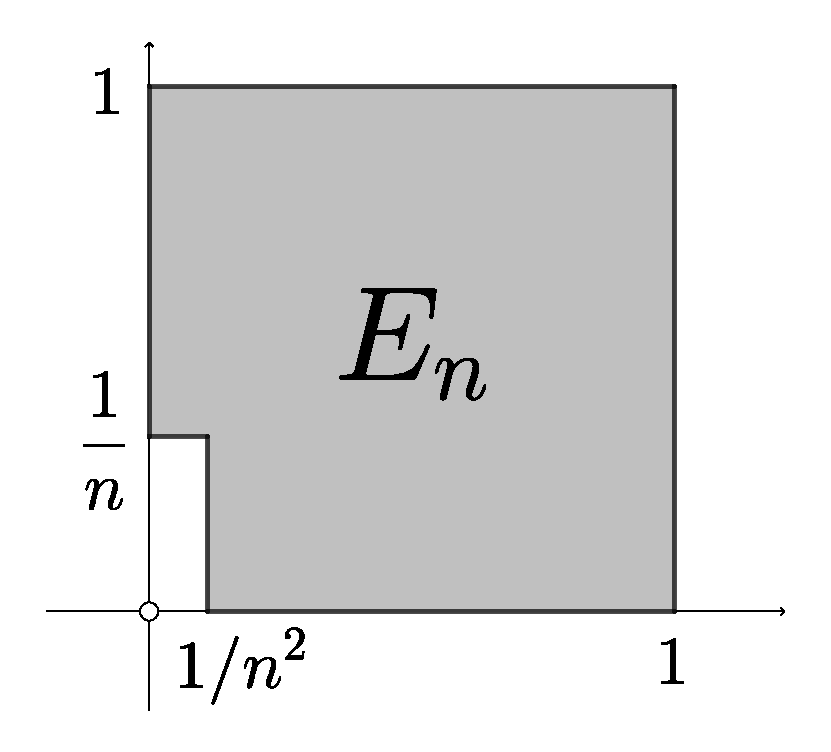
\includegraphics[width=4.8cm]{10/collong.pdf}\\
     $D_n = D-\left( \left[0, \frac{1}{n}\right) \times \left[0, \frac{1}{n^2}\right) \right)$ &
     $E_n = D-\left( \left[0, \frac{1}{n^2}\right) \times \left[0, \frac{1}{n}\right) \right)$
   \end{tabular}
 \end{figure}
 
 このとき,以下のように増加近似列の選び方によって極限値が異なる.
 \begin{align*}
   \iint_{D_n} \frac{x-y}{(x+y)^3}\ dx dy 
   &= \int_{0}^{\frac{1}{n}}\left( \int_{\frac{1}{n^2}}^{1}\frac{x-y}{(x+y)^3}\ dy \right) dx 
     + \int_{\frac{1}{n}}^{1}\left( \int_{0}^{1}\frac{x-y}{(x+y)^3}\ dy \right) dx\\[1ex]
   &= \int_{0}^{\frac{1}{n}}\left[\frac{y}{(x+y)^2}\right]_{y=\frac{1}{n^2}}^{y=1}\ dx 
     + \int_{\frac{1}{n}}^{1} \left[ \frac{y}{(x+y)^2}\right]_{y=0}^{y=1}\ dx\\[1ex]
   &= \int_{0}^{\frac{1}{n}}\left( \frac{1}{(x+1)^2} - \frac{1/n^2}{(x+1/n^2)^2}\right) dx 
   + \int_{\frac{1}{n}}^{1} \frac{dx}{(x+1)^2}\\[1ex]
   &= \frac{1}{2} - \frac{1}{1+1/n} \to -\frac{1}{2} \; (n \to \infty)\\[1ex]
   \iint_{E_n} \frac{x-y}{(x+y)^3}\ dx dy
   &=\int_{0}^{\frac{1}{n^2}}\left( \int_{\frac{1}{n}}^{1}\frac{x-y}{(x+y)^3}\ dy \right) dx
     + \int_{\frac{1}{n^2}}^{1}\left( \int_{0}^{1}\frac{x-y}{(x+y)^3}\ dy \right) dx\\[1ex]
   &=\int_{0}^{\frac{1}{n^2}}\left[ \frac{y}{(x+y)^2}\right]_{y=\frac{1}{n}}^{1}\ dx
     + \int_{\frac{1}{n^2}}^{1} \left[ \frac{y}{(x+y)^2}\right]_{y=0}^{y=1}\ dx\\[1ex]
   &=\int_{0}^{\frac{1}{n^2}}\left( \frac{1}{(x+1)^2} - \frac{1/n}{(x+1/n)^2}\right) dx
     + \int_{\frac{1}{n^2}}^{1}\frac{dx}{(x+1)^2}\ dx\\[1ex]
   &= \frac{1}{2} - \frac{1}{n+1} \to \frac{1}{2} \; (n \to \infty)
 \end{align*}
 これより広義積分 $\ds \iint_{D} \frac{x-y}{(x+y)^3}\ dx dy$ は発散す
 る.
 \newpage
 
 先程の例のように,広義2重積分
 \begin{equation}\label{eq:improper-int}
   \iint_{D} f(x,y) \ dx dy
 \end{equation}
 において,$D$ で $f(x,y)>0$ となることも $f(x,y)<0$ となることもある場
 合は定理\ref{thm:improper-conv}は使えず,1個の増加近似列に関する極限を
 調べるだけでは不十分であり,あらゆる増加近似列に対して同じ極限値に収束
 するかどうかを調べる必要がある.このような場合は,まず被積分関数 $f$ に対して
 \begin{equation}\label{eq:f_pm}
   f_{+}(x,y) := \left\{
     \begin{array}{cl}
       f(x,y) & \left( f(x,y) \geqq 0 \right)\\[1ex]
       0 & \left( f(x,y) \leqq 0\right)
     \end{array}
   \right. \qquad
   f_{-}(x,y) := \left\{
     \begin{array}{cl}
       0 & \left( f(x,y) \geqq 0\right)\\[1ex]
       -f(x,y) & \left( f(x,y) \leqq 0 \right)
     \end{array}
   \right.
 \end{equation}
 として,$f(x,y)$ を
 \[
   f(x,y) = f_{+}(x,y) - f_{-}(x,y)
 \]
 と分ける.$D$ 上で $f_{+}(x,y)\geqq 0 , \; f_{-}(x,y) \geqq 0$ なので,
 定理\ref{thm:improper-conv}から広義2重積分
 \begin{equation}\label{eq:improper-pm}
   \iint_{D}f_{+}(x,y) \ dxdy, \qquad \iint_{D}f_{-}(x,y) \ dxdy
 \end{equation}
 の収束・発散はそれぞれ $D$ の1個の増加近似列について極限を調べればよい.
 これらのいずれもが収束するとき,広義2重積分 (\ref{eq:improper-int}) は
 収束し,以下が成り立つ.
 \[
   \iint_{D} f(x,y) \ dx dy = \iint_{D}f_{+}(x,y) \ dx dy - \iint_{D} f_{-}(x,y) \ dx
 \]
 一方,(\ref{eq:improper-pm})のどちらか一方でも発散すれば広義
 積分 (\ref{eq:improper-int}) は発散する.以上を定理としてまとめる.

 \begin{theorem}\label{thm:improper-criterion} 広義2重積分
   $\ds \iint_{D} f(x,y) \ dxdy$ の収束に関して次が成り立つ.
   \[
     \iint_{D} f(x,y) \ dx dy \text{ は収束する } \quad
     \Longleftrightarrow \quad \iint_{D}f_{+}(x,y) \ dxdy, \; \iint_{D}f_{-}(x,y) \ dxdy \text{ が
       共に収束する}
   \]
   さらに,広義2重積分 $\ds \iint_{D}f(x,y) \ dxdy$ が収束するとき,以下が成り立つ.
   \[
     \iint_{D}f(x,y) \ dx dy = \iint_{D}f_{+}(x,y) \ dxdy - \iint_{D} f_{-}(x,y) \ dxdy
   \]
 \end{theorem}

 なお,広義2重積分の収束・発散を判定するのみであれば,次の定理を根拠として $|f(x,y)|$ の広義
 2重積分の収束・発散を定理\ref{thm:improper-conv}を使って判定してもよい.

 \begin{theorem}
   広義2重積分 $\ds \iint_{D} f(x,y) \ dxdy$ の収束に関して次が成り立つ.
   \[
     \iint_{D}f(x,y) \ dx dy \text{ は収束する } \quad
     \Longleftrightarrow \quad \iint_{D}|f(x,y)| \ dxdy \text{ は収束する }
   \]
   特に,広義2重積分 $\ds \iint_{D}|f(x,y)| \ dxdy$ が収束するとき,以下が成り立つ.
   \[
     \iint_{D} |f(x,y)| \ dxdy = \iint_{D} f_{+}(x,y) \ dx dy + \iint_{D} f_{-}(x,y) \ dxdy
   \]
 \end{theorem}
 
 前々ページで例として挙げた,以下の広義2重積分の収束・発散を定理\ref{thm:improper-criterion}を使っ
 て判定してみる.
 \[
   \iint_{D} \frac{x-y}{(x+y)^3} \ dx dy \qquad D=\Set{(x,y) \ \mid \
     0 \leqq x \leqq 1, \; 0 \leqq y \leqq 1, \; (x,y) \neq (0,0)}
 \]
 被積分関数に $f(x,y)$ と名前をつければ,(\ref{eq:f_pm}) の $f_{+}, f_{-}$ はそれぞれ
 \[
   f_{+}(x,y) = \left\{
     \begin{array}{cl}
       \dfrac{x-y}{(x+y)^3} & ( x \geqq y)\\[1ex]
       0 & ( x \leqq y)
     \end{array}
   \right. \qquad f_{-}(x,y) = \left\{
     \begin{array}{cl}
       0 & (x \geqq y)\\[1ex]
       -\dfrac{x-y}{(x+y)^3} & (x \leqq y)
     \end{array}
   \right.
 \]
 である.そこで,
 \[
   D^{+}:= D \cap \Set{(x,y) \ \mid \ x \geqq y}  \qquad D^{-}:= D \cap \Set{(x,y) \ \mid \ x \leqq y}
 \]
 とすれば,$\ds D = D^{+} \cup D^{-}$ であり,$D^{+} \cap D^{-}$ の面積は $0$ なので
 \[
   \begin{aligned}
     \iint_{D} f^{+}(x,y) \ dxdy &= \iint_{D^{+}} \frac{x-y}{(x+y)^3} \ dxdy + \iint_{D^{-}} 0 \ dx dy
                                   = \iint_{D^{+}} f(x,y) \ dxdy\\[1ex]
     \iint_{D} f^{-}(x,y) \ dxdy &= \iint_{D^{+}} 0 \ dxdy  + \iint_{D^{-}} -\frac{x-y}{(x+y)^3} \ dxdy
                                   = -\iint_{D^{-}} f(x,y) \ dxdy
   \end{aligned}
 \]
 である.従って,$D^{+}, D^{-}$ 上での $f(x,y)$ の広義2重積分の収束・発
 散を調べればよい.\\

 まず,$D^{+}$ 上での $f(x,y)$ の広義2重積分の収束・発散を調べる.$D^{+}$ 上で $f(x,y) \geqq 0$ であり,
 \[
   D^{+}_{n} := \Set{(x,y) \ | \ \frac{1}{n} \leqq x \leqq
     1, \; 0 \leqq y \leqq x} \; (n \geqq 2)
 \]
 とすれば $\Set{D^{+}_n}$ は $D^{+}$ の増加近似列なので,定理\ref{thm:improper-conv}から極限
 \[
   \lim_{n \to \infty} \iint_{D^{+}_{n}} \frac{x-y}{(x+y)^3} \ dxdy
 \]
 が収束するか $+\infty$ に発散するかを判定すればよい.
 \[
   \begin{aligned}
     \iint_{D^{+}_n} f(x,y) \ dxdy
     &= \int_{\frac{1}{n}}^{1} \left( \int_{0}^{x} \frac{x-y}{(x+y)^3} \ dy \right) dx
       = \int_{\frac{1}{n}}^{1}\left[ \frac{y}{(x+y)^2}\right]_{y=0}^{y=x} \ dx
       = \int_{\frac{1}{n}}^{1} \frac{dx}{4x}\\[1ex]
     & = \frac{\log n}{4} \to +\infty \; (n \to \infty)
   \end{aligned}
 \]
 なので,広義2重積分 $\ds \iint_{D^{+}} f(x,y) \ dxdy$ は発散する.よっ
 て,$D^{-}$ 上の広義2重積分を調べるまでもなく,定理\ref{thm:improper-criterion}から広義2重積分
 $\ds \iint_{D} \frac{x-y}{(x+y)^3} \ dxdy$ は発散することがわかる.\\

 ちなみに,$D^{-}$ 上の広義2重積分 $\ds \iint_{D^{-}} f(x,y) \
 dxdy$ も $+\infty$ に発散することが同様の計算で確かめられる.



\end{document}


\documentclass[10pt, uplatex, dvipdfmx]{jsarticle}
\usepackage{../mypackage} 

\graphicspath{{../pictures}} 

\setcounter{section}{10}

\begin{document}

\section{Gauss 積分と誤差関数}

\subsection{Gauss 積分}

以下の広義積分は\textbf{Gauss 積分}と呼ばれる.この値を広義2重積分を使って求める.
\[
  \int_{-\infty}^{\infty} e^{-x^2} \ dx
\]

\vspace{1zh}

まず,この広義積分 $I$ が収束することを確認しておく.開区間上の広義積分の定義に従って
\begin{equation}\label{eq:gauss-divide}
  \int_{-\infty}^{\infty} e^{-x^2} \ dx  = \int_{-\infty}^{0} e^{-x^2} \ dx + \int_{0}^{\infty} e^{-x^2} \ dx
\end{equation}
と分けて,右辺の2個の広義積分がいずれも収束することを示す.ここで,$u=-x$ としての置換積分により
\begin{equation}\label{eq:gauss-L}
  \int_{-\infty}^{0} e^{-x^2} \ dx = \lim_{c \to -\infty} \int_{c}^{0} e^{-x^2} \ dx
  = \lim_{c \to -\infty} \int_{-c}^{0} -e^{-u^2} \ du = \lim_{c \to \infty} \int_{0}^{-c} e^{-x^2} \ dx
  =\int_{0}^{\infty} e^{-x^2} \ dx
\end{equation}
なので,(\ref{eq:gauss-divide})の右辺第2項が収束することを示せばよい.さらに,
\begin{equation}\label{eq:gauss-R}
  \int_{0}^{\infty} e^{-x^2} \ dx = \int_{0}^{1} e^{-x^2} \ dx + \int_{1}^{\infty} e^{-x^2} \ dx
\end{equation}
と分ければ,この右辺第1項は通常の積分なので第2項が収束することを示せばよい.$x \in [1, \infty)$ に対して
\[
  \left| e^{-x^2} \right| = e^{-x^2} \leqq x e^{-x^2}
\]
である.さらに,この最右辺の $[1,\infty)$ 上の広義積分は以下のように収束する.
\[
  \int_{1}^{\infty} x e^{-x^2} \ dx = \lim_{c \to \infty} \int_{1}^{c}
  x e^{-x^2} \ dx = \lim_{c \to \infty} \left[
    -\frac{e^{-x^2}}{2}\right]_{1}^{c} = \lim_{c \to \infty}
  \frac{e^{-1} - e^{-c^2}}{2} = \frac{e^{-1}}{2}
\]
よって,(\ref{eq:gauss-R})の右辺第2項の
広義積分は収束するので,Gauss 積分は収束する.\\

上記の通り Gauss 積分は収束するので,以下が成り立つ.
\[
  \int_{-\infty}^{\infty} e^{-x^2} \ dx  = \lim_{n \to \infty} \int_{-n}^{n} e^{-x^2} \ dx
\]
なお,一般には
\[
  \int_{-\infty}^{\infty} f(x) \ dx \text{ と } \lim_{n \to \infty} \int_{-n}^{n} f(x) \ dx
\]
は別物だが,広義積分 $\ds \int_{-\infty}^{\infty} f(x) \ dx$ が収束する
なら,両者は等しい.従って,以下が成り立つ.
\begin{equation}\label{eq:gauss-square}
  \begin{aligned}
    \left( \int_{-\infty}^{\infty} e^{-x^2} \ dx \right)^2
    &= \left( \lim_{n \to \infty} \int_{-n}^{n} e^{-x^2} \ dx \right)^2
      = \lim_{n \to \infty} \left( \int_{-n}^{n} e^{-x^2} \ dx\right)^2\\[1ex]
    & = \lim_{n \to \infty} \left( \int_{-n}^{n} e^{-x^2} \ dx \right) \left( \int_{-n}^{n} e^{-y^2} \ dy \right)
      = \lim_{n \to \infty} \int_{-n}^{n} \left( \int_{-n}^{n} e^{-x^2-y^2} \ dx \right) dy\\[1ex]
    &= \lim_{n \to \infty} \iint_{[-n,n] \times [-n,n]} e^{-x^2-y^2} \ dx dy
  \end{aligned}
\end{equation}
ここで,$D_n = [-n,n] \times [-n,n]$ とおけ
ば,$\Set{D_n}$ は $\mathbb{R}^2$ の増加近似列である.任意の $(x,y)
\in \mathbb{R}^2$ に対して
$e^{-x^2-y^2}>0$ なので,(\ref{eq:gauss-square})から以下が成り立つ.
\begin{equation}
  \left( \int_{-\infty}^{\infty} e^{-x^2} \ dx \right)^2 = \iint_{\mathbb{R}^2} e^{-x^2-y^2} \ dx dy
\end{equation}
この右辺の広義2重積分の値を求める.これが収束することは既にわかっている
ので,$\mathbb{R}^2$ の増加近似列として計算しやすいものを選べばよい.
\[
  E_n = \Set{(x,y) \ \mid \ x^2+y^2 \leqq n^2}
\]
とすれば,$\Set{E_n}$ は $\mathbb{R}^2$ の増加近似列なので
\[
  \iint_{\mathbb{R}^2} e^{-x^2-y^2} \ dx dy = \lim_{n \to \infty} \iint_{E_n} e^{-x^2-y^2} \ dx dy
\]
である.極座標変換 $x=r\cos\theta, \; y=r\sin\theta$ によって,$r\theta$ 平面の閉領域
\[
  F_n = \Set{(r, \theta) \ \mid \ 0 \leqq r \leqq n, \; 0 \leqq \theta \leqq 2\pi}
\]
が $xy$ 平面の $E_n$ に変換される.極座標変換の Jacobian は $J(r,\theta)=r$ なので,
\[
  \begin{aligned}
    \iint_{E_n} e^{-x^2-y^2} \ dx dy
    &= \iint_{F_n} e^{-r^2} |J(r,\theta)| \ dr d\theta
      = \int_{0}^{2\pi} \left( \int_{0}^{n} r e^{-r^2} \ dr \right) d\theta\\[1ex]
    & = \left( \int_{0}^{2\pi} d\theta\right) \left( \int_{0}^{n} r e^{-r^2} \ dr\right)
      = 2\pi \left[ -\frac{e^{-r^2}}{2}\right]_{0}^{n} = \pi \left( 1 - e^{-n^2}\right)
  \end{aligned}
\]
である.よって,以下を得る.
\[
  \iint_{\mathbb{R}^2} e^{-x^2-y^2} \ dx dy = \lim_{n \to \infty} \pi \left( 1-e^{-n^2}\right) = \pi
\]
これと(\ref{eq:gauss-square})から
$\ds \left( \int_{-\infty}^{\infty} e^{-x^2} \ dx \right)^2 = \pi$ であ
り,明らかに $\ds \int_{-\infty}^{\infty} e^{-x^2} \ dx >0$ なので,Gauss積分の値は
\begin{equation}\label{eq:gauss-int}
  \fbox{$\ds \int_{-\infty}^{\infty} e^{-x^2} \ dx = \sqrt{\pi}$}
\end{equation}
である.さらに,(\ref{eq:gauss-divide})と(\ref{eq:gauss-L})から
\[
  \int_{-\infty}^{\infty} e^{-x^2} \ dx = 2 \int_{0}^{\infty} e^{-x^2} \ dx
\]
なので,(\ref{eq:gauss-int})と合わせて以下も得られる.
\begin{equation}\label{eq:gauss-half}
  \fbox{$\ds \int_{0}^{\infty} e^{-x^2} \ dx = \frac{\sqrt{\pi}}{2}$}
\end{equation}
次に紹介する誤差関数$\ds \erf x = \frac{2}{\sqrt{\pi}}\int_{0}^{x}
e^{-t^2} \ dt$ に$\ds \frac{2}{\sqrt{\pi}}$ という定数が含まれているの
はこの(\ref{eq:gauss-half})が理由である.つまり,$\ds \lim_{x \to
  \infty} \erf x = 1$ となって欲しいからである.

\newpage

\subsection{誤差関数}

\end{document}


\addtocontents{toc}{\newpage}

\documentclass[10pt, uplatex, dvipdfmx]{jsarticle}
\usepackage{../mypackage}

\graphicspath{{../pictures}}

\setcounter{section}{11}

\begin{document}


\section{体積と面積と曲面積}

 \subsection{2重積分と体積}
 
 \begin{theorem}\label{thm:volume}
  $f,g$ を有界閉領域 $D \subset \mathbb{R}^2$ 上重積分可能な関数と
  し,$D$ 上で $f(x,y) \geqq g(x,y)$ とする.$D$ から $xy$ 平面に垂直に
  生やした柱と曲面 $z=f(x,y)$ と $z=g(x,y)$
  で囲まれた立体
  \[
    V=\Set{ (x,y,z) | (x,y) \in D, \, g(x,y) \leqq z \leqq
      f(x,y)}
  \]
  の体積は2重積分 $\ds \iint_{D} \Big( f(x,y) - g(x,y) \Big) dx dy$ に等しい.
  \begin{figure}[h]
    \centering
    \includegraphics[height=6cm]{07/monotonic.png}
  \end{figure}
\end{theorem}

\begin{example}\label{ex:volsphere}
  半径 $R>0$ の球の体積 $V(R)$ は $D=\Set{(x,y) | x^2+y^2 \leqq R^2}$ 上
  の以下の2重積分で求められる.
  \begin{align*}
    V(R) &= \iint_{D} \left( \sqrt{R^2-x^2-y^2} - \left(-\sqrt{R^2-x^2-y^2}\right)\right) dx dy\\
         & = 2\iint_{E} r\sqrt{R^2-r^2}\  dr d\theta 
           \quad \Big( E=\Set{(r, \theta) | 0 \leq r \leq R, \, 0 \leq \theta \leq 2\pi}\Big)\\
         & = 2 \int_{0}^{2\pi} \left( \int_{0}^{R} r \sqrt{R^2-r^2} \ dr \right) d\theta
           = 4\pi \left[ -\frac{1}{3} \left(R^2-r^2\right)^{\frac{3}{2}}\right]_{r=0}^{r=R}
           =\frac{4}{3}\pi R^3
  \end{align*}
  \begin{figure}[h]
    \centering
    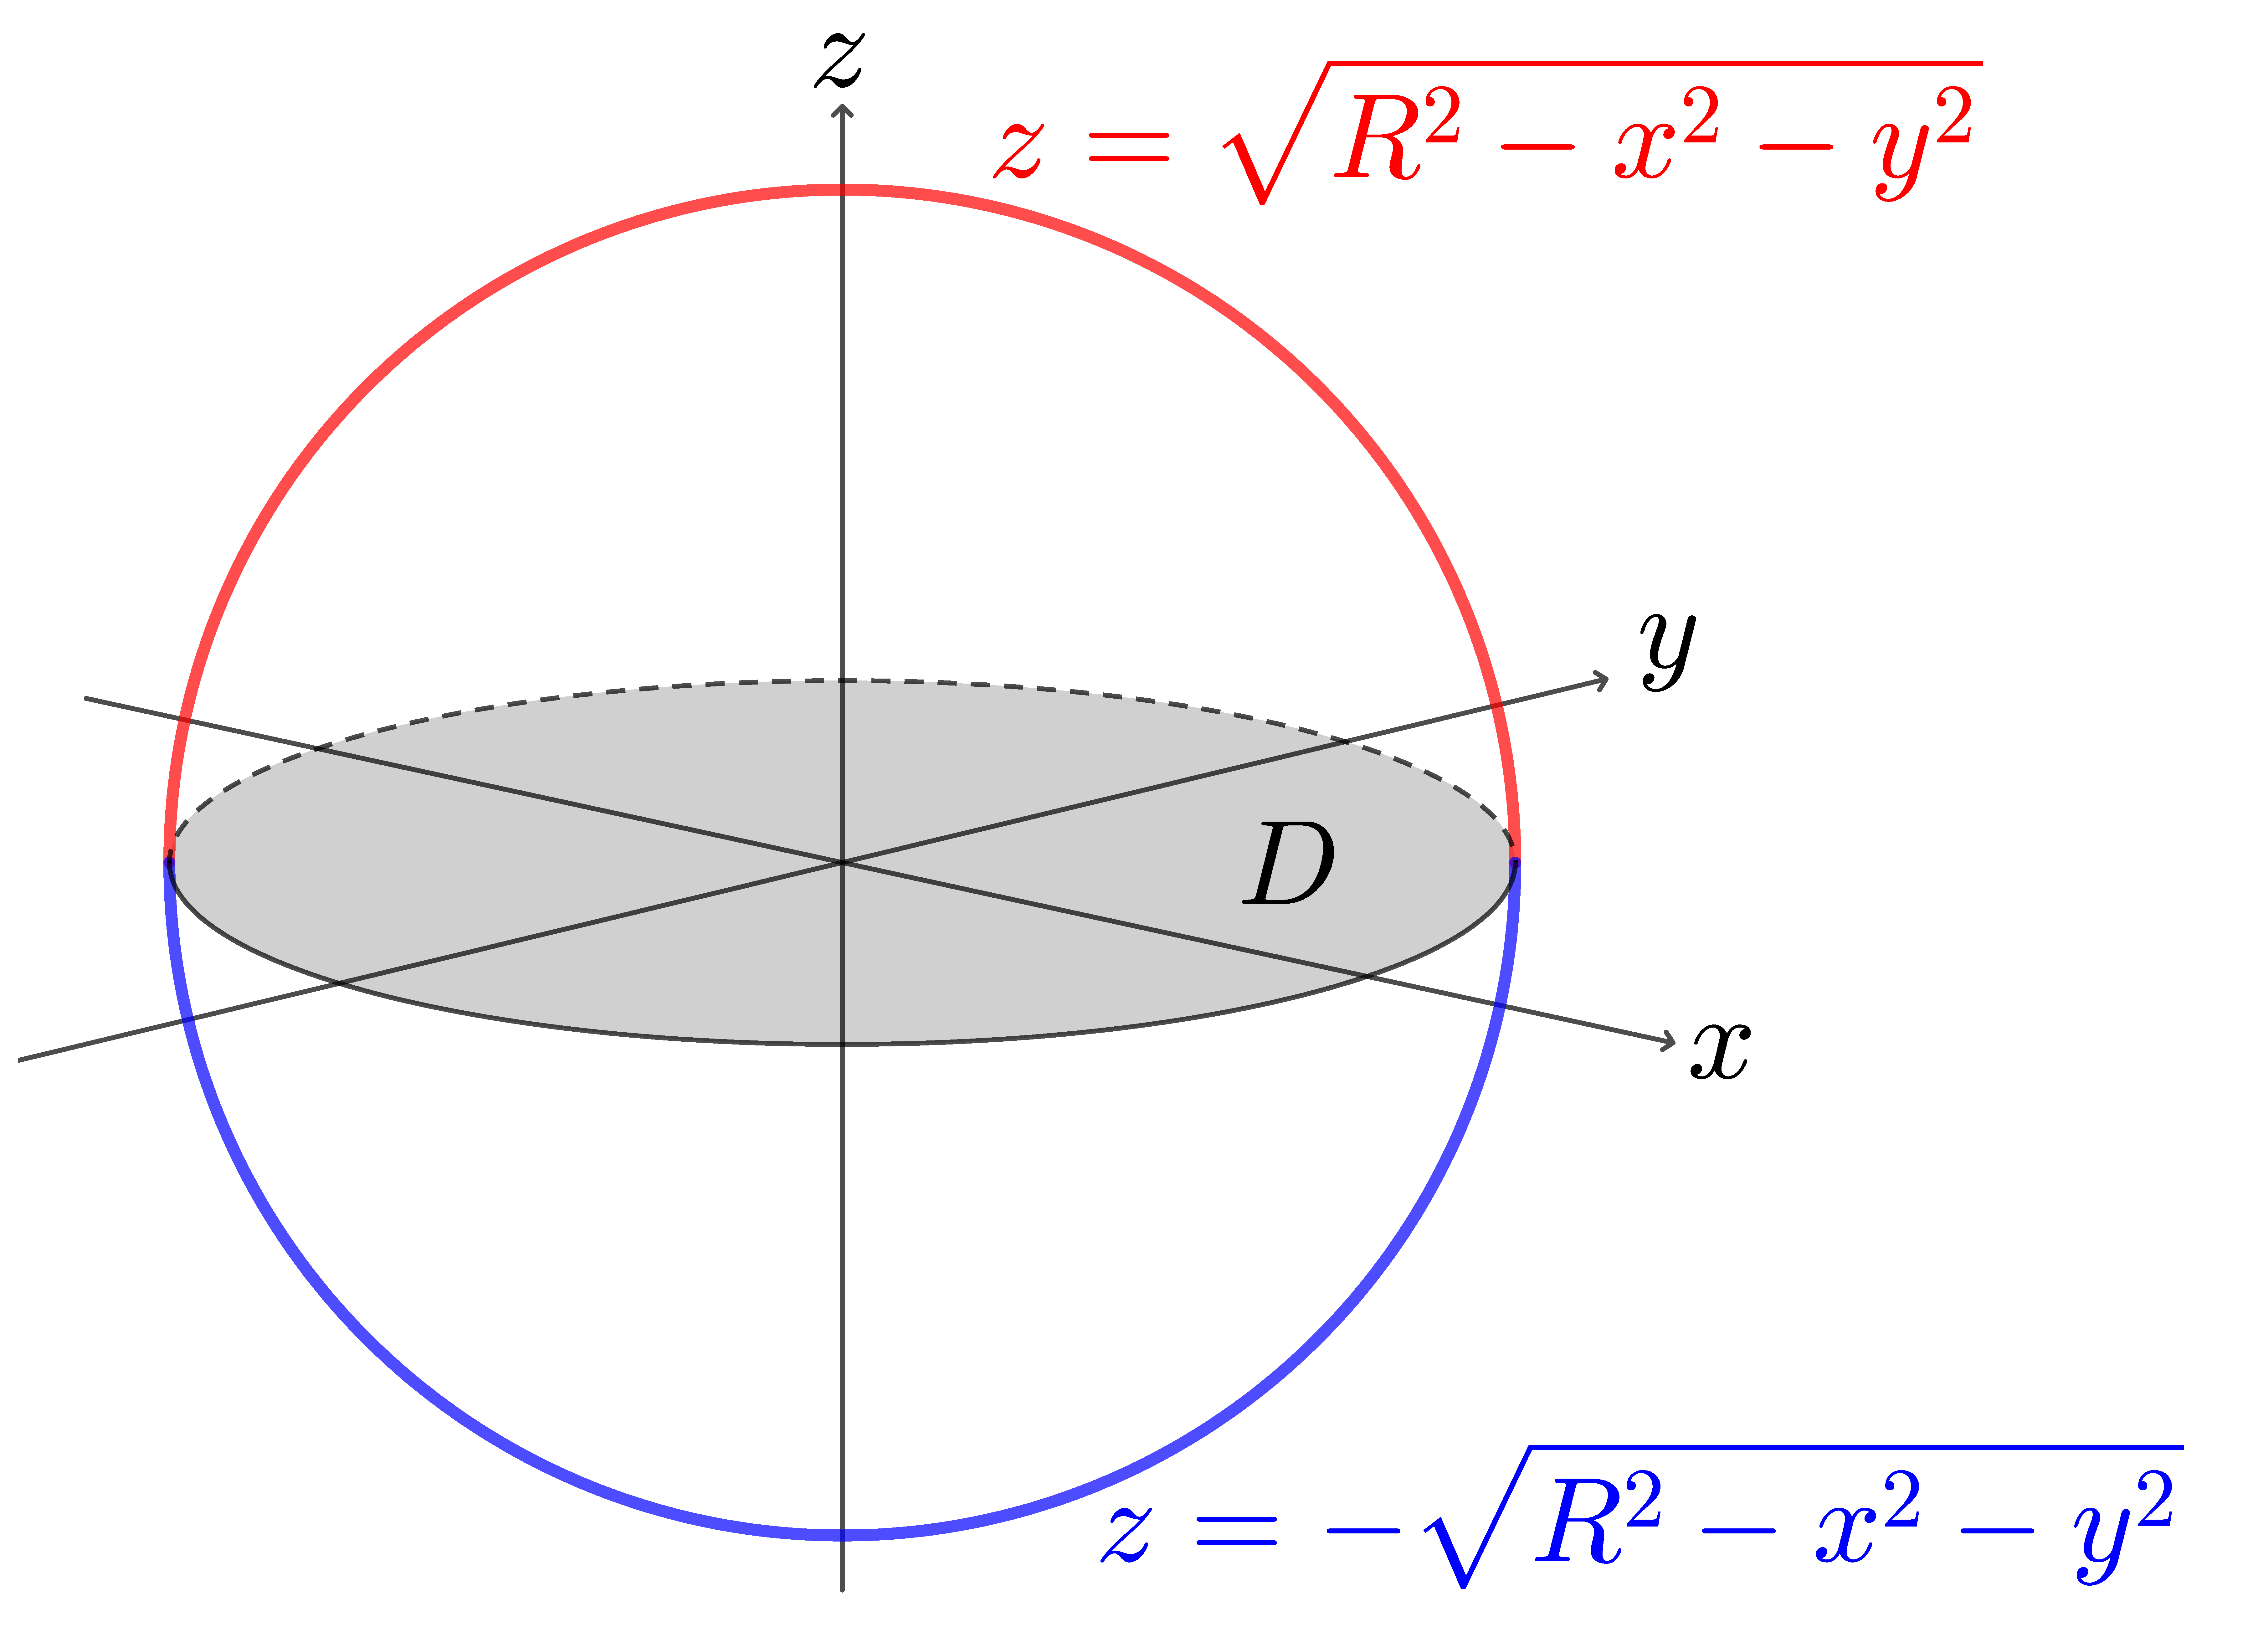
\includegraphics[height=5cm]{12/sphere2d.pdf}
  \end{figure}
\end{example}

\begin{example}
  下図のような曲面 $z=x^2+y^2$ と平面 $z=2x$ で囲まれる立体の体積を求める.
  \begin{figure}[h]
    \centering
    \includegraphics[width=10cm]{12/cutparab.png}
  \end{figure}

  平面 $z=2x$ が曲面 $z=x^2+y^2$ より上部にある閉
  領域上で2重積分を計算すればよい.つまり,
  \[
    D= \Set{(x,y) \ \mid x^2+y^2 \leqq 2x}
  \]
  として,2重積分 $\ds \iint_{D} \left( 2x - \left(x^2+y^2\right) \right) \ dx dy$ を計算する.\\

  簡単な不等式の変形により,$D$ は点 $(1,0)$ を中心とする半径 $1$ の円板であるこ
  とがわかる.そこで,極座標変換と $x$ 方向の平行移動を合成した変
  換
  \[
    \begin{cases}
      x = r\cos \theta+1\\
      y = r\sin \theta
    \end{cases}
  \]
  を使う.この変換によって $r\theta$ の閉領域
  \[
    E = \Set{(r, \theta) \ \mid \ 0 \leqq r \leqq 1, \; 0 \leqq \theta \leqq 2\pi}
  \]
  が $D$ に変換される.変換の Jacobian は
  \[
    J(r,\theta) = \left|
      \begin{array}{cc}
        \frac{\partial x}{\partial r} & \frac{\partial x}{\partial \theta}\\[1ex]
        \frac{\partial y}{\partial r} & \frac{\partial y}{\partial \theta}
      \end{array}
    \right| = \left|
      \begin{array}{rr}
        \cos \theta & -r\sin\theta\\[1ex]
        \sin \theta & r\cos\theta
      \end{array}
    \right| = r
  \]
  なので,求めたい体積は次のように計算できる.
  \[
    \iint_{D} \left( 2x- \left(x^2+y^2\right) \right) \ dx dy
    = \iint_{E} \left(1-r^2\right) r \ dr d\theta 
    = \int_{0}^{2\pi}\left( \int_{0}^{1} \left(r-r^3\right)dr \right) d\theta = \frac{\pi}{2}
  \]
\end{example}

\newpage

\subsection{2重積分と面積}

$xy$ 平面内の有界閉領域 $D$ を底面とする高さ $1$ の立体の体積は $D$ の
面積に等しい.

\begin{theorem}\label{thm:doublearea}
  定数関数が重積分可能な有界閉領域 $D$ の面積は2重積分 $\ds \iint_{D}dxdy$ の値に等しい.
  \begin{figure}[h]
    \centering
    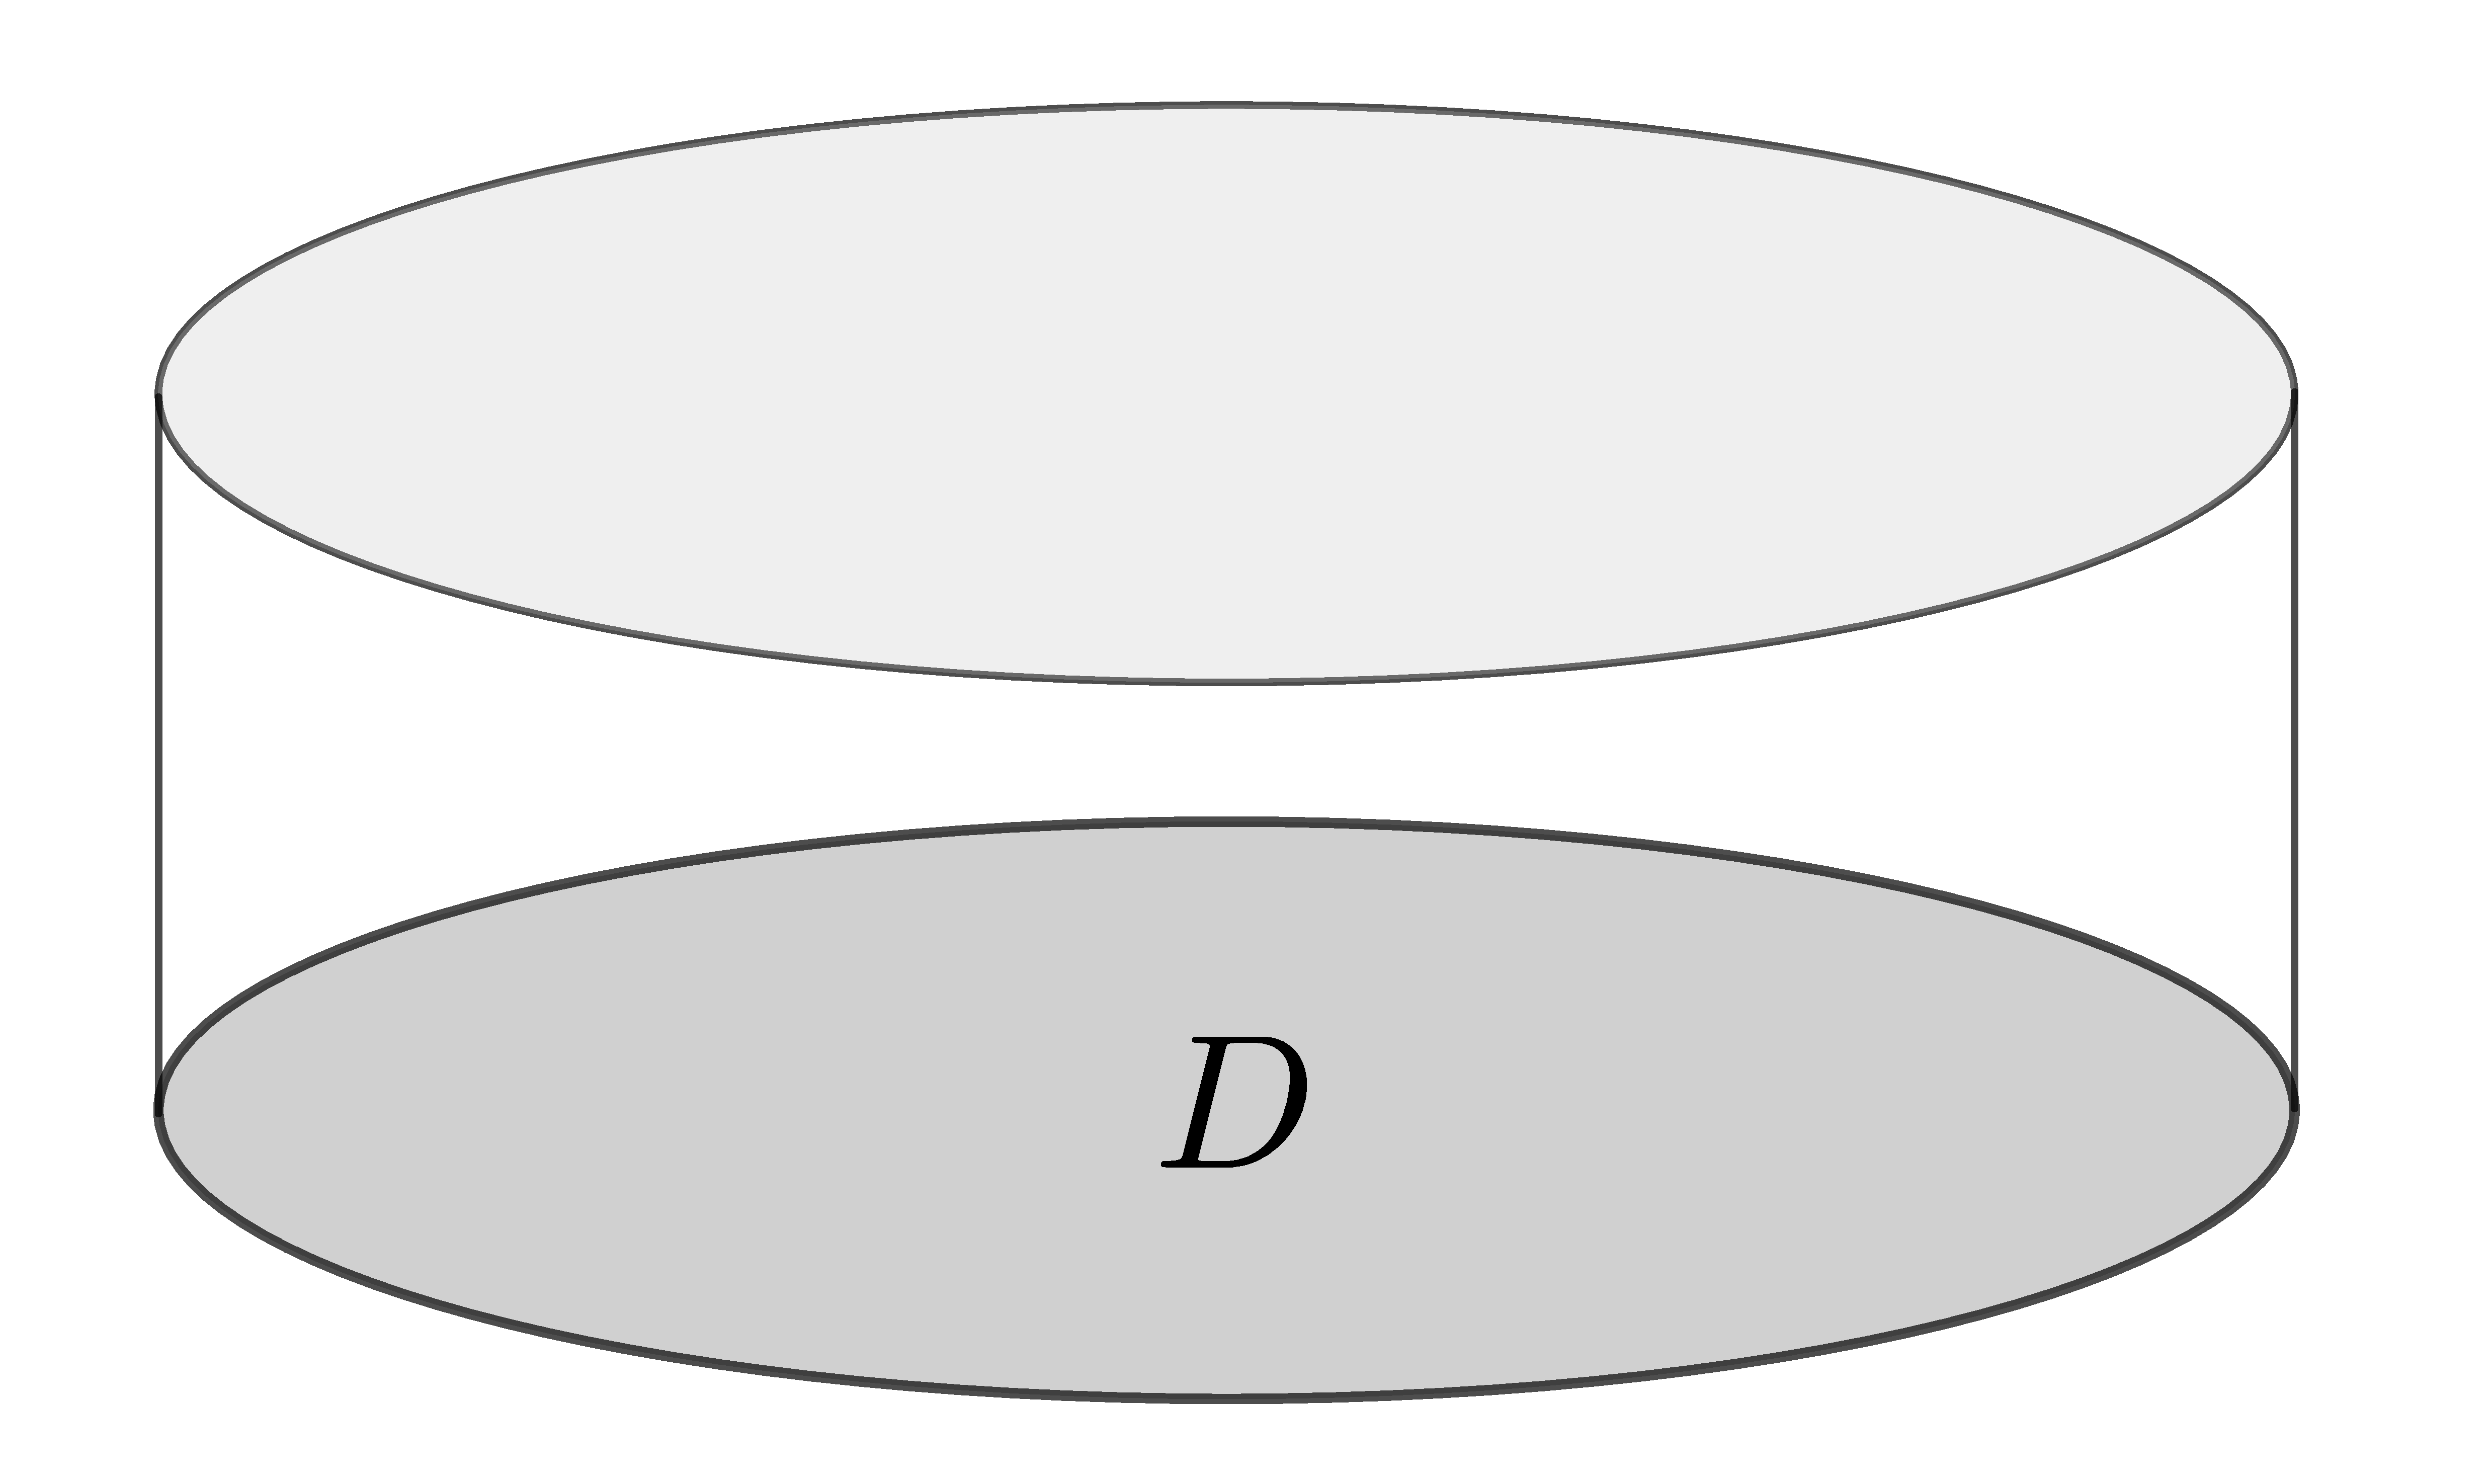
\includegraphics[width=10cm]{12/volume-area.pdf}
  \end{figure}
\end{theorem}

\begin{example}
  半径 $R>0$ の円の面積 $S(R)$ は $1$ 変数関数の積分で求められるが,定
  理\ref{thm:doublearea}より
  \[
    D=\Set{(x,y) | x^2+y^2 \leqq R}
  \]
  上で定数関数の$2$ 重積分を計算しても求められる.
  \[
    S(R) = \iint_{D} dx dy = \int_{-R}^{R} \left(\int_{-\sqrt{R^2-x^2}}^{\sqrt{R^2-x^2}} dy \right) dx
    = \int_{-R}^{R} \left( \sqrt{R^2-x^2} - \left(-\sqrt{R^2-x^2} \right) \right) \ dx = \pi R^2
  \]
\end{example}

\vspace{1zh}

この例を見てわかるように,定理\ref{thm:doublearea}を使ったからといって
特に計算が楽になる訳でもなく,途中からこれまで通りの1変数の積分計算に合
流している.より一般に,有界閉領域 $D$ が縦線集合として
\[
  D=\Set{(x,y) \ \mid \ a \leqq x \leqq b, \; \varphi_1(x) \leqq y \leqq \varphi_2(x)}
\]
と書けるなら $D$ 上の定数関数 $z=1$ の2重積分は次のように計算される.
\[
  \iint_{D} dx dy = \int_{a}^{b} \left( \int_{\varphi_1(x)}^{\varphi_2(x)} \ dy \right) dx
  = \int_{b}^{a} \Big( \varphi_2(x) - \varphi_1(x) \Big) \ dx
\]
これは結局 $y=\varphi_1(x)$ と $y=\varphi_2(x)$ と $x=a$ と $x=b$ で囲
まれる平面図形 $D$ の面積を求める積分である.$D$ が横線集合として書ける
ときも全く同様である.\\

「だから定理\ref{thm:doublearea}なんて意味がない」と主張したい
訳\textbf{ではない}.むしろこの定理によって定数関数の2重積分に面積という意味
付けが与えられる.

\newpage

\subsection{立体の断面積と積分と体積}

立体の断面積を積分すればその立体の体積が得られる.

\begin{theorem}\label{thm:area-section}
  $xyz$ 空間にある立体を $x$ 軸に垂直な平面 $x=\xi$ で切断したときの断
  面積が $S(\xi)$ であり,この立体が $a\leqq x \leqq b$ の範囲に含
  まれているとする.関数 $S(x)$ が有界閉区間 $[a,b]$ で積分可能な
  ら,この立体図形の体積は以下の積分値に等しい.
  \[
    \int_{a}^{b} S(x) \ dx
  \]
  \begin{figure}[h]
    \vspace{-1cm}
    \centering
    \includegraphics[height=5cm]{12/section.pdf}
  \end{figure}
\end{theorem}


\begin{remark}
  当たり前だが,$x$ 軸だけに限らず $y$ 軸や $z$ 軸についてもこの定理と
  同様のことが成り立つ.さらには,座標軸だけに限らず空間の任意の直
  線とそれに垂直な平面での断面積に関して同様のことが成り立つ.
\end{remark}

\begin{example}
  放物線 $y=x^2$ を $x$ 軸の周りで回転させて得られる回転体の $0 \leqq
  x \leqq 1$ の部分の体積を求める.
  
  \begin{figure}[h]
    \centering
    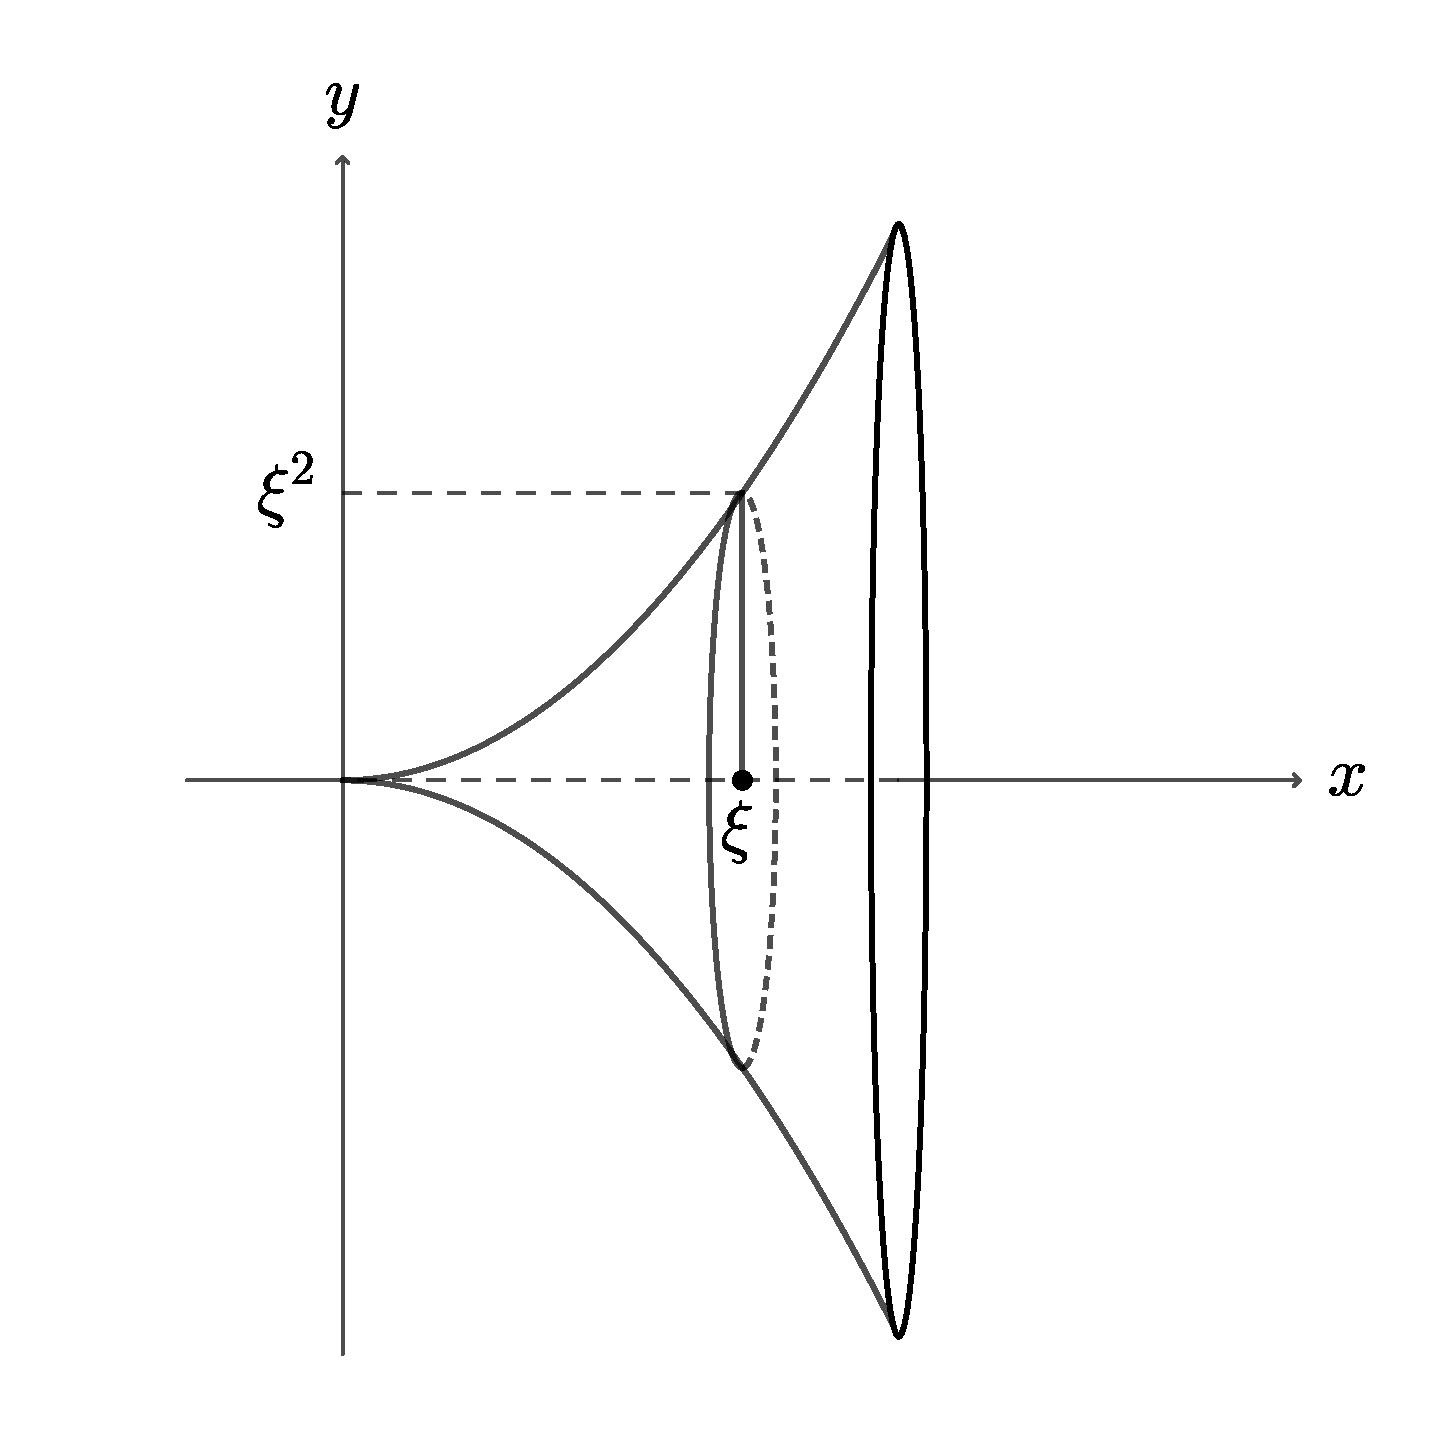
\includegraphics[height=7cm]{12/revolution.pdf}
  \end{figure}

  \noindent
  この立体を平面 $x=\xi$ で切断したと
  きの断面は半径 $\xi^2$ の円なので,その面積は $\pi \xi^4$ である.
  従って,定理\ref{thm:area-section}からこの立体の体積は以下のように計
  算できる.
  \[
    \int_{0}^{1} \pi x^4 \ dx = \pi \left[ \frac{x^5}{5}\right]_{0}^{1} = \frac{\pi}{5}
  \]

\end{example}
\newpage

\subsection{曲面積}


$\varphi, \psi, \chi$ を $uv$ 平面内の有界閉領域 $D$ 上定義され
た $C^1$ 級関数とする.点 $(u,v)$ が $D$ を動くとき,$xyz$ 空間内の
点 $\left( \varphi(u,v), \psi(u,v), \chi(u,v)\right)$ はなめらかな曲
面 $S$ を描く.これを
\[
  x=\varphi(u,v), \; y=\psi(u,v), \; z=\chi(u,v), \; (u,v) \in D
\]
と書き,曲面 $S$ の\textbf{媒介変数表示}という.

\begin{theorem}\label{thm:surface-area}
  有界閉領域 $D$ 上の $C^1$ 級関数 $\varphi, \psi, \chi$ によって媒介変
  数表示される曲面の面積は
  \[
    \iint_{D} \sqrt{\left( \frac{D(x,y)}{D(u,v)}\right)^2 + \left( \frac{D(y,z)}{D(u,v)}\right)^2 
      + \left( \frac{D(z,x)}{D(u,v)}\right)^2} \ du dv
  \]
  に等しい.ただし,ここで
  \[
    \frac{D(x,y)}{D(u,v)} = \left|
      \begin{array}{cc}
        x_u & x_v\\
        y_u & y_v
      \end{array}
    \right|, \quad \frac{D(y,z)}{D(u,v)} = \left|
      \begin{array}{cc}
        y_u & y_v\\
        z_u & z_v
      \end{array}
    \right|, \quad \frac{D(z,x)}{D(u,v)} = \left|
      \begin{array}{cc}
        z_u & z_v\\
        x_u & x_v
      \end{array}
    \right|
  \]
  であり,被積分関数は $D$ 上重積分可能であるとする.
\end{theorem}

\begin{example}
  半径 $R >0$ の球面は以下の媒介変数表示で与えられる.
  \[
    x = R\cos\theta  \cos \varphi, \quad
    y= R \sin \theta \cos\varphi, \quad
    z = R \sin \varphi, \quad 
    0\leqq \theta \leqq 2\pi, \; -\frac{\pi}{2} \leqq \varphi \leqq \frac{\pi}{2}
  \]
  \begin{figure}[h]
    \vspace{-2.5zh}
    \centering
    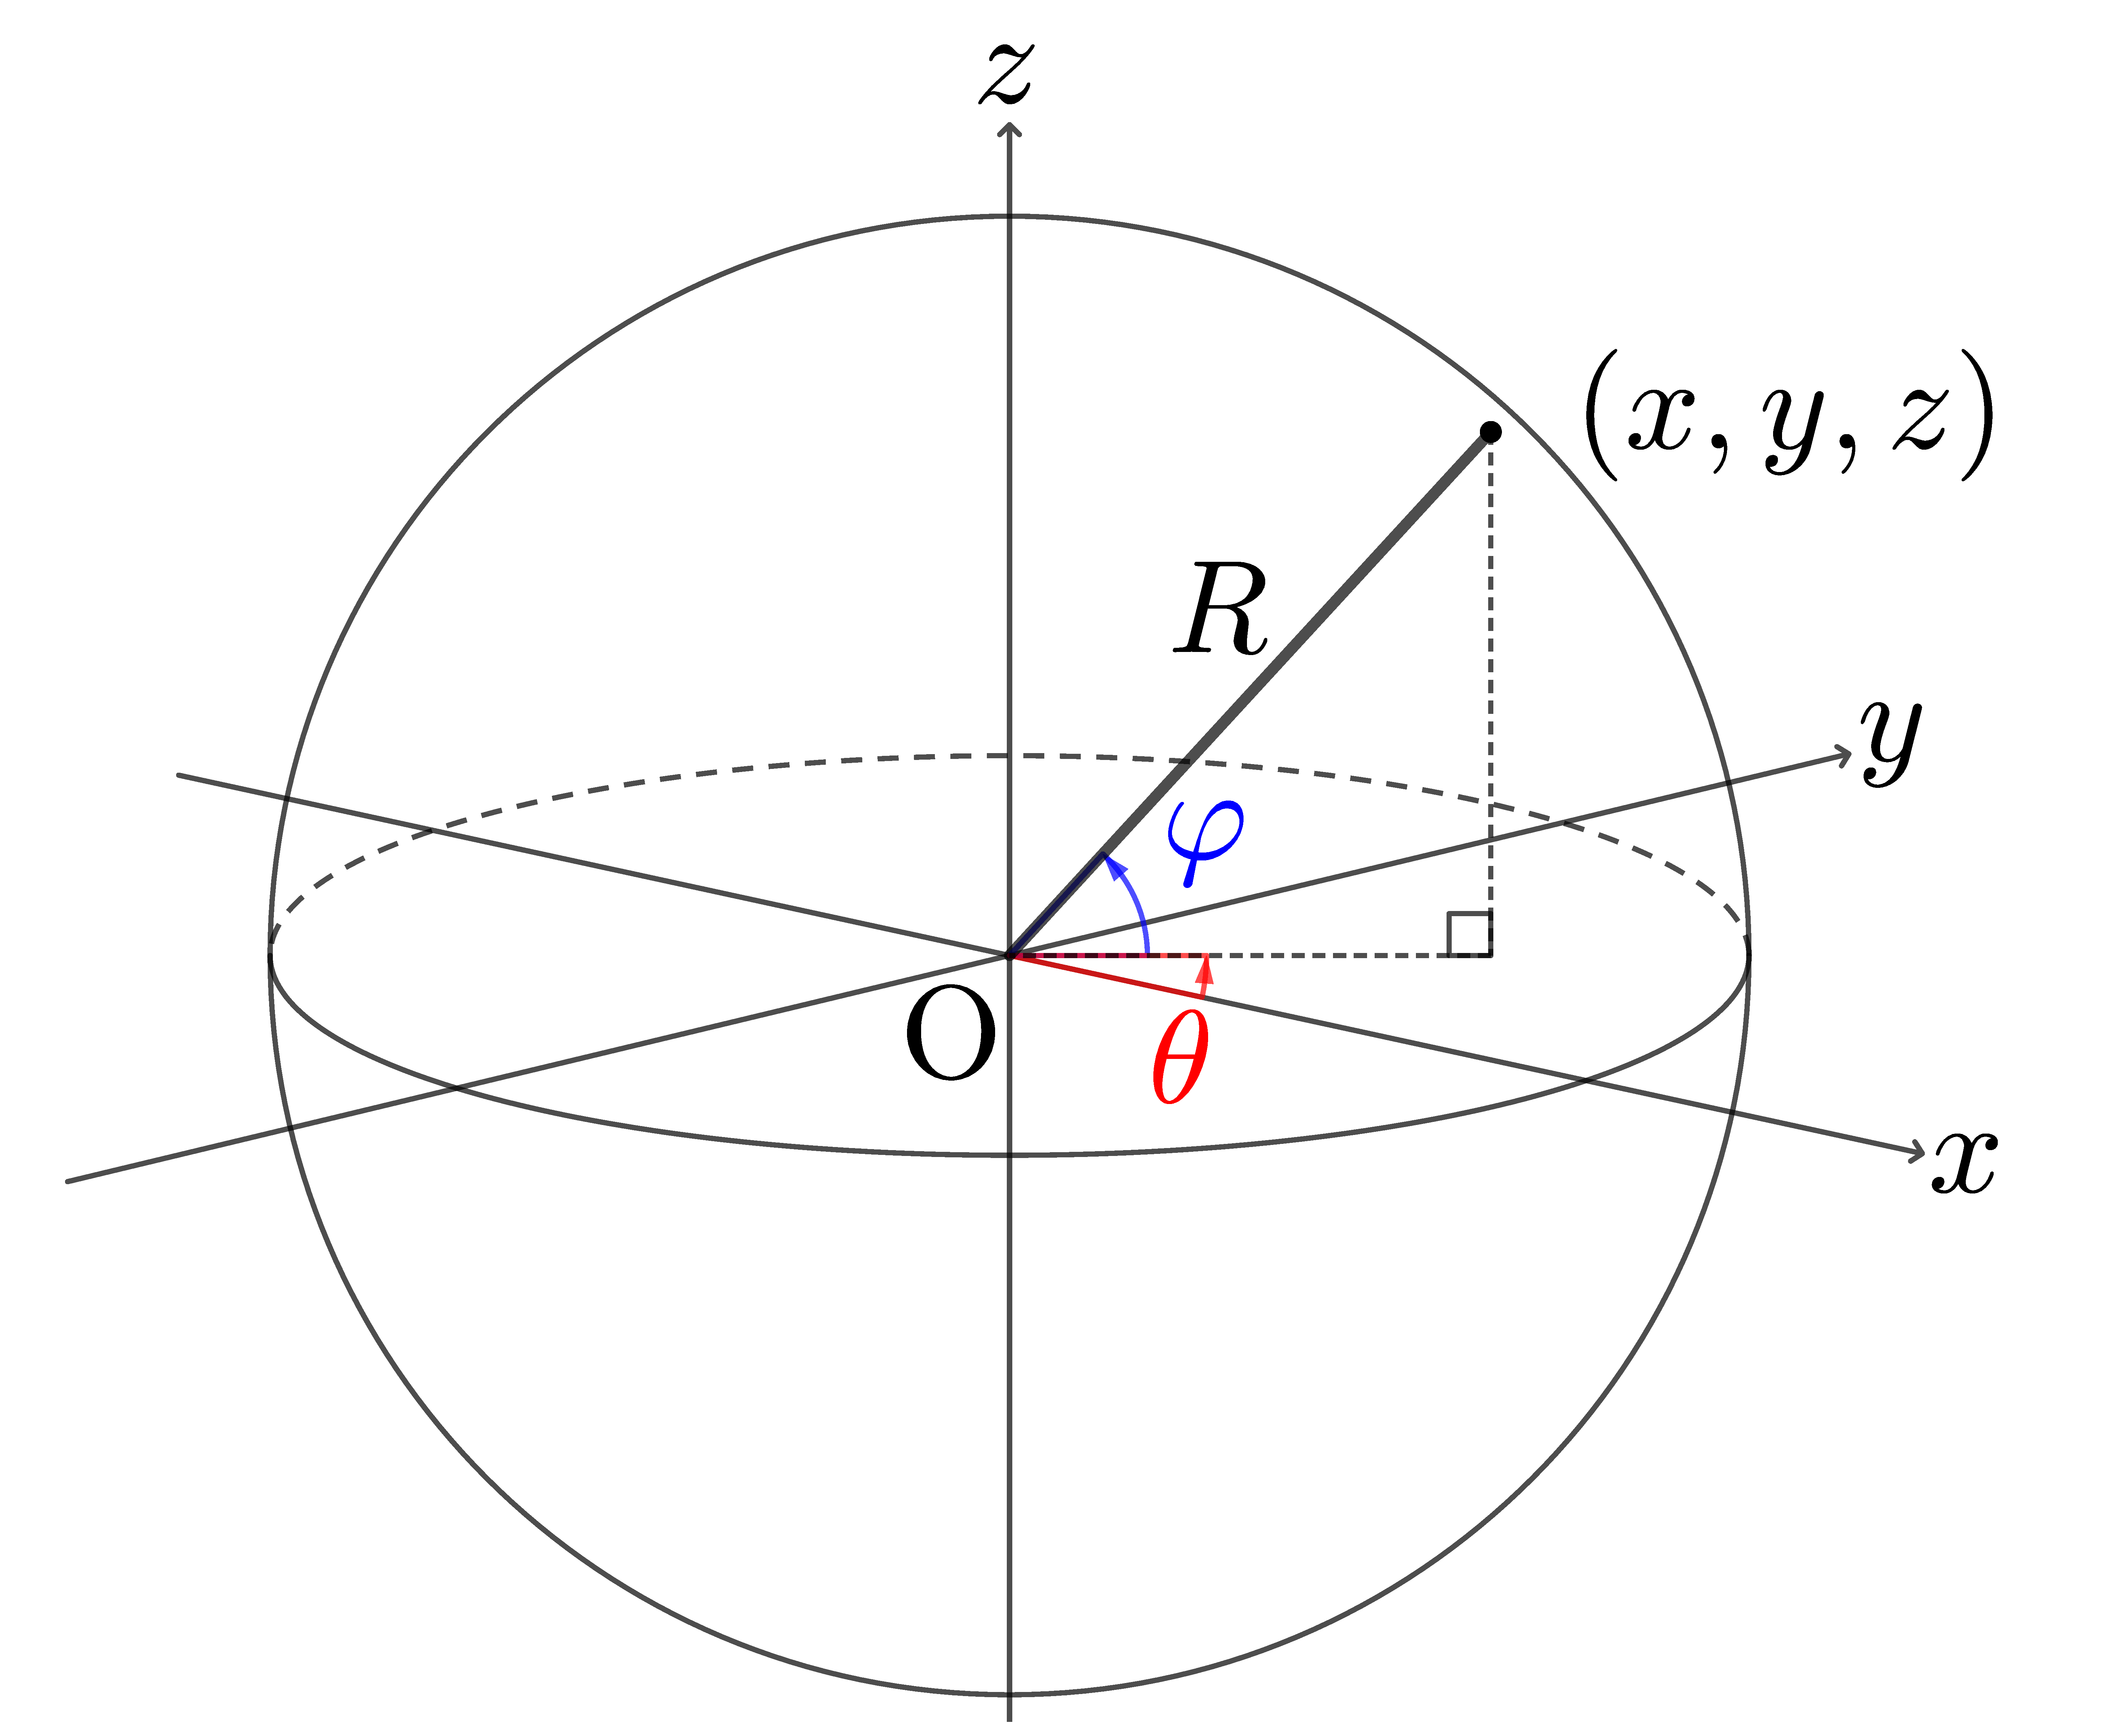
\includegraphics[height=4.7cm]{12/pole3d.pdf}
  \end{figure}

  曲面積の計算に必要な3個の Jacobian は以下の通りである.
  \[
    \begin{aligned}
    \frac{D(x,y)}{D(\theta, \varphi)} &= \left|
             \begin{array}{cc}
               x_{\theta} & x_{\varphi}\\
               y_{\theta} & y_{\varphi}
             \end{array}
           \right| = \left|
             \begin{array}{rr}
               -R \sin\theta \cos\varphi & -R \cos\theta \sin \varphi\\
               R \cos\theta \cos\varphi & -R \sin\theta \sin\varphi
             \end{array}
           \right| = R^2 \cos\varphi\sin\varphi\\[1ex]
      \frac{D(y,z)}{D(\theta, \varphi)} &= \left|
                                          \begin{array}{cc}
                                            y_{\theta} & y_{\varphi}\\
                                            z_{\theta} & z_{\varphi}
                                          \end{array}
                                          \right|= \left|
                                          \begin{array}{cc}
                                            R\cos\theta \cos\varphi & -R\sin\theta\sin\varphi\\
                                            0 & R\cos\varphi
                                          \end{array}
                                          \right| = R^2 \cos\theta \cos^2\varphi\\[1ex]
      \frac{D(z,x)}{D(\theta,\varphi)} &=\left|
                                        \begin{array}{cc}
                                          z_{\theta} & z_{\varphi}\\
                                          x_{\theta} & z_{\varphi}
                                        \end{array}
                                        \right| = \left|
                                         \begin{array}{cc}
                                           0 & R\cos\varphi\\
                                           -R\sin\theta\cos\varphi & -R\cos\theta\sin\varphi
                                         \end{array}
                                         \right| = R^2 \sin\theta \cos^2\varphi
    \end{aligned}
  \]
  これより半径 $R$ の球の表面積 $S(R)$ は
  $\ds D= \left[ 0, 2\pi \right] \times \left[ -\frac{\pi}{2},
    \frac{\pi}{2}\right]$ 上の2重積分として以下のように計算できる.
  \[
    \begin{aligned}
      S(R) &= \iint_{D} \sqrt{\left( \frac{D(x,y)}{D(\theta, \varphi)}\right)^2
             +\left( \frac{D(y,z)}{D(\theta,\varphi)}\right)^2 + \left( \frac{D(z,x)}{D(\theta,\varphi)}\right)^2
             } d\theta d\varphi
             = \iint_{D}R^2 \left|\cos \varphi\right| \ d\theta d\varphi\\
           &=R^2 \left( \int_{0}^{2\pi}d\theta\right)\left(\int_{-\frac{\pi}{2}}^{\frac{\pi}{2}}\cos\varphi\ d\varphi\right)
             = 4\pi R^2
    \end{aligned}
  \]
  
\end{example}

$C^1$ 級関数 $z=f(x,y)$ のグラフとして与えられる曲面は
\[
  x=u, \; y=v, \; z=f(u,v), \; (u,v) \in D
\]
と媒介変数表示できる.このとき
\[
  \frac{D(x,y)}{D(u,v)} = \left|
    \begin{array}{cc}
      1 & 0\\
      0 & 1
    \end{array}
    \right| = 1, \quad \frac{D(y,z)}{D(u,v)} = \left|
      \begin{array}{cc}
        0 & 1\\
        f_x & f_y
      \end{array}
    \right| = -f_x, \quad \frac{D(z,x)}{D(u,v)} = \left|
      \begin{array}{cc}
        f_x & f_y\\
        1 & 0
      \end{array}
    \right| = -f_y
\]
なので,定理\ref{thm:surface-area}の特別な場合として以下の定理が得られる.

\begin{theorem}\label{thm:function-area}
  有界閉領域 $D$ 上の $C^1$ 級関数 $z=f(x,y)$ のグラフの曲面積は以下の
  積分で与えられる.ただし,被積分関数は $D$ 上重積分可能であるとする.
  \[
    \iint_{D} \sqrt{ 1 + f_x(x,y)^2 + f_y(x,y)^2} \ dx dy
  \]
\end{theorem}

\begin{example}
  半径 $R>0$ の球の表面積 $S(R)$ は,2変数関数 $z=\sqrt{R^2-x^2-y^2}$の
  グラフの曲面積の $2$
  倍なので,$D=\Set{(x,y) | x^2+y^2 < R^2}$上の広義2重積分として以下の
  ようにも計算できる.
  \[
    S(R) = 2\iint_{D}\sqrt{ 1 + {z_x}^2 + {z_y}^2} \ dx dy 
    =  2R \iint_{D} \frac{dxdy}{\sqrt{R^2-x^2-y^2}} = 4\pi R^2
  \]
\end{example}

\begin{example}
  放物線をその軸の周りで回転して得られる回転放物面 $z=x^2+y^2$ の $x^2+y^2
  \leqq 1$ の部分の表面積を求める.つまり,$D=\Set{(x,y) \ \mid \
    x^2+y^2 \leqq 1}$ として,以下の2重積分を計算する.
  \[
    \iint_{D} \sqrt{1+z_x^2 + z_y^2} \ dx dy = \iint_{D} \sqrt{1+4x^2+4y^2} \ dx dy
  \]
  極座標変換 $x=r\cos\theta, y=r\sin\theta$ によって,$r\theta$ 平面の
  \[
    E = \Set{(r, \theta) \ \mid \ 0 \leqq r \leqq 1, \; 0 \leqq 0 \leqq 2\pi}
  \]
  が $xy$ 平面の $D$ に変換される.極座標変換の Jacobian は $J(r,\theta)=r$ なので,以下のように計算できる.
  \[
    \begin{aligned}
      \iint_{D} \sqrt{1+4x^2+4y^2} \ dx dy
      &= \iint_{E} \sqrt{1+4r^2} ~| J(r, \theta)| \ dr d\theta
        = \left(\int_{0}^{2\pi}\ d\theta\right) \left( \int_{0}^{1} r \sqrt{1+4r^2} \ dr \right)\\[1ex]
      &= 2\pi \left[ \frac{1}{12} \left( 1+4r^2\right)^{\frac{3}{2}}\right]_{0}^{1}
        = \frac{\pi\left(5\sqrt{5}-1\right)}{6}
    \end{aligned}
  \]
  \begin{figure}[h]
    \centering
    \includegraphics[height=4cm]{12/paraboloid.pdf}
  \end{figure}
\end{example}


\end{document}


\documentclass[10pt, uplatex, dvipdfmx]{jsarticle}
\usepackage{../mypackage} 

\graphicspath{{../pictures}} 

\setcounter{section}{12}

\begin{document}

\section{ 3重積分}

3変数関数の積分を定義する.一般の多変数関数の積分も同様に定義できる.

\subsection{3重積分の定義}

$f$ を直方体 $K=[a,a'] \times [b,b'] \times [c,c'] \subset
\mathbb{R}^3$ で定義された有界な $3$ 変数関数とする.$K$ の各方向を以下
のように分割する.
\begin{align*}
  \Delta :
  \begin{array}{l}
    a = x_0 < x_1 < \cdots < x_l = a'\\
    b = y_0 < y_1 < \cdots < y_m = b'\\
    c = z_0 < z_1 < \cdots < z_n = c'
  \end{array}
\end{align*}
これにより,直方体 $K$ は $lmn$ 個の直方体
\[
  K_{ijk} = [x_{i-1}, x_{i}] \times [y_{j-1},y_j] \times [z_{k-1}, z_k]
\]
に分割され,各 $K_{ijk}$ の体積は
$|K_{ijk}|=(x_i - x_{i-1})(y_j - y_{j-1})(z_k - z_{k-1})$ である.各直
方体から代表点 $(\xi_{ijk}, \eta_{ijk}, \zeta_{ijk}) \in K_{ijk}$ を選ぶ.このとき,
\[
  R(\Delta, \Set{ (\xi_{ijk}, \eta_{ijk}, \zeta_{ijk})}, f) 
  := \sum_{i=1}^{l} \sum_{j=1}^{m} \sum_{k=1}^{n} f(\xi_{ijk}, \eta_{ijk}, \zeta_{ijk}) |K_{ijk}|
\]
を分割 $\Delta$ と代表点集合 $\Set{(\xi_{ijk}, \eta_{ijk}, \zeta_{ijk})}$ に関する $f$ の Riemann 和という.
\[
  |\Delta| := \max_{i, j, k}\Set{ x_i-x_{i-1}, \, y_j-y_{j-1}, \, z_k-z_{k-1}}
\]
とする.$|\Delta| \to 0$ のとき,分割の仕方と代表点集合の取り方によら
ず Riemann 和が一定の値に収束するならば,$f$ は $K$ で\textbf{(Riemann)重積分積
  分可能}であるという.その極限値を
\[
  \iiint_{K} f(x,y,z) \ dxdydz
\]
で表し,$f$ の $K$ 上の\textbf{3重積分}という.一般の集合 $V \subset
\mathbb{R}^3$ 上の有界関数 $f$ の3重積分は,$V$ を含む直方体 $K$ を1つ
とり,
\[
  f^*(x,y,z) = \left\{
    \begin{array}{c l}
      f(x,y,z) & \left( (x,y,z) \in V\right)\\
      0 & \left( (x,y,z) \notin V\right)
    \end{array}
  \right.
\]
として,$f^{*}$ $K$ で重積分可能なら $f$ は $V$ で重積分可能であるとし,
\[
  \iiint_{V} f(x,y,z)\ dx dy dz = \iiint_{K} f^*(x,y,z)\ dx dy dz
\]
によって $f$ の $V$ 上の3重積分を定義する.この値は $V$ を含む直方体 $K$ の選び方によらない.

\begin{theorem}
  $\mathbb{R}^3$ の有界な直方体 $V$ 上の連続関数は3重積分可能である.
\end{theorem}

\newpage

\subsection{3重積分の計算方法}

3重積分を2重積分に帰着させて計算する方法を紹介する.

\begin{theorem}\label{thm:iterated3}
  平面 $\mathbb{R}^2$ の有界閉領域 $D$ 上定義された2変数関数
  $\varphi_1, \varphi_2 \; (\varphi_1(x,y) \leq \varphi_2(x,y))$ によって
  \[
    V=\Set{(x,y,z) | (x,y) \in D, \, \varphi_1(x,y) \leqq z \leqq \varphi_2(x,y)}
  \]
  と表せる集合 $V$ 上で3重積分可能な関数 $f$ に対して以下が成り立つ.
  \[
    \iiint_V f(x,y,z) \ dx dy dz = \iint_{D} \left(
      \int_{\varphi_1(x,y)}^{\varphi_2(x,y)} f(x,y,z)\ dz\right) dxdy
  \]
\end{theorem}


\begin{example}
  次の3重積分を計算する.
  \[
    \iiint_V \frac{dxdydz}{(1+x+y+z)^3} \qquad
    V= \Set{(x,y,z) \ \mid \ x+y+z \leqq 1, \; x \geqq 0, \; y\geqq 0, \; z \geqq 0}
  \]
  $V$ は平面 $x+y+z=1$ で空間を2分割したときの原点 $\mathrm{O}(0,0,0)$
  を含む側であって,各座標が $0$ 以上の部分である.平
  面 $x+y+z=1$ は3点
  $\mathrm{A}(1,0,0), \; \mathrm{B}(0,1,0), \; \mathrm{C}(0,0,1)$ を通
  る平面なので,$V$ は四面体 OABC
  の内側である.
  \begin{figure}[h]
    \centering
    \includegraphics[height=6cm]{13/tetrahedron.pdf}
  \end{figure}
  
  \noindent 従って,$D=\Set{(x,y) \ \mid \ x+y \leqq 1, \; x \geqq
    0, \; y\geqq 0} \; \left(\subset \mathbb{R}^2\right)$ とすれば
  \[
    V = \Set{(x,y,z) \ \mid \ (x,y) \in D, \; 0 \leqq z \leqq 1-x-y}
  \]
  と書ける.よって,定理\ref{thm:iterated3}によって次のように計算できる.
  \[
    \begin{aligned}
      \iiint_{V} \frac{dxdydz}{(1+x+y+z)^3}
      &= \iint_{D}\left( \int_{0}^{1-x-y} \frac{dz}{(1+x+y+z)^3} \right) \ dx dy\\[1ex]
      &  = \iint_{D} \left[ -\frac{1}{2(1+x+y+z)^2} \right]_{z=0}^{z=1-x-y} \ dx dy\\[1ex]
      &  = \iint_{D}\left( \frac{1}{2(1+x+y)^2} - \frac{1}{8}\right) \ dx dy = \frac{1}{2}\log 2 - \frac{5}{16}
    \end{aligned}
  \]
\end{example}

\subsection{変数変換}

2重積分と同様に,適切な変数変換によってより計算しやすい3重積分に書き直せることがある.

\begin{theorem}
  変数変換
  \[
    x=\varphi(u,v,w), \; y=\psi(u,v,w), \; z=\chi(u,v,w) \quad (\varphi, \psi, \chi \text{ は $C^1$ 級})
  \]
  によって,$xyz$ 空間の $V$ と $uvw$ 空間の $W$ が1対1に対応し,$(u,v,w) \in W$ に対して
  \[
    J(u,v,w) := \left|
      \begin{array}{ccc}
        x_{u} & x_{v} & x_{w}\\
        y_{u} & y_{v} & y_{w}\\
        z_{u} & z_{u} & z_{w}
      \end{array}
    \right| \neq 0 \quad \left( J(u,v,w) \text{ は Jacobian と呼ばれる} \right)
  \]
  とする.このとき,3変数関数 $f$ が $V$ 上重積分可能なら以下が成り立つ.
  \begin{equation}\label{eq:trans-3d}
    \iiint_V f(x,y,z) \ dxdydz 
    = \iiint_W f\left( \varphi(u,v,w), \psi(u,v,w), \chi(u,v,w)\right) |J(u,v,w)|\ du dv dw
  \end{equation}
\end{theorem}

\begin{remark}
  2重積分のときと同様に,上の定理の条件はもう少し緩められる.例え
  ば,3次元の極座標変換
  \[
    x=r\cos \theta \cos \varphi, \; y=r\sin\theta \cos\varphi, \; z=r\sin\varphi
  \]
  はよく用いられる変数変換である.
  \begin{figure}[h]
    \centering
    \includegraphics[height=5cm]{13/trans-pole3d.pdf}
  \end{figure}
  
  \noindent これは $r\theta\varphi$ 空間の
  \[
    W=\Set{(r,\theta,\varphi) | 0 \leqq r \leqq R, \, 0 \leqq \theta \leqq 2\pi, \;
      -\frac{\pi}{2} \leqq \varphi \leqq \frac{\pi}{2}}
  \]
  を $xyz$ 空間の $V=\Set{(x,y,z) | x^2+y^2+z^2=R^2}$ に変換する
  が,1対1の対応ではない.しかしながら,\uwave{$W$ から体積 $0$ の部分集合を適
    切に除けば1対1に対応する}.また,この変換の Jacobian は
  \[
    J(r, \theta, \varphi) = \left|
      \begin{array}{ccc}
        \cos \theta \cos \varphi & -r\sin\theta \cos\varphi & -r\cos\theta\sin\varphi\\
        \sin \theta \cos \varphi & r\cos\theta \cos\varphi & -r\sin\theta\sin\varphi\\
        \sin\varphi & 0 & r\cos\varphi
      \end{array}
    \right| = r^2\cos\varphi
  \]
  であるが,これも \uwave{$W$ から体積 $0$ の部分集合を適切に除いたとこ
    ろで $J \neq 0$ である}( 具体的には $W$ から部
  分集合 $\Set{(r, \theta, \varphi) \ \mid \ r=0 \text{ または }
    \cos \varphi=0}$ を除けばよい).この例のように,2つの波線部を満たしていれ
  ば(\ref{eq:trans-3d}) が成り立つ.
\end{remark}

\begin{example}\label{exmp:trans-pole3d}
  半径 $R \; (>0)$ の球
  $V=\Set{(x,y,z) \ \mid \ x^2+y^2+z^2 \leqq R^2}$ 上の次の3重積
  分を計算する.
  \[
    \iiint_V dx dy dz
  \]
  先ほど説明した通り,3次元の極座標変換
  \[
    x = r \cos\theta \cos \varphi, \quad y = r\sin\theta\cos\varphi,
    \quad z=r\sin\varphi
  \]
  によって,$r\theta\varphi$ 空間の
  \[
    W=\Set{((r,\theta,\varphi) \ \mid \ 0 \leqq r \leqq R, \; 0 \leqq
      \theta \leqq 2\pi, \; -\frac{\pi}{2} \leqq \varphi \leqq \frac{\pi}{2}}
  \]
  が $xyz$ 空間の $V$ に変換される.変換
  の Jacobian は
  \[
    J(r, \theta, \varphi) = \left|
      \begin{array}{ccc}
        \cos \theta \cos \varphi & -r\sin\theta \cos\varphi & -r\cos\theta\sin\varphi\\
        \sin \theta \cos \varphi & r\cos\theta \cos\varphi & -r\sin\theta\sin\varphi\\
        \sin\varphi & 0 & r\cos\varphi
      \end{array}
    \right| = r^2\cos\varphi
  \]
  なので,(\ref{eq:trans-3d}) を適用して次のように計算できる.
  \[
    \begin{aligned}
      \iiint_{V} dx dy dz
      &= \iiint_{W} |J(r, \theta, \varphi)| \ dr d\theta d\varphi
        = \left( \int_{0}^{R} r^2 \ dr\right) \left( \int_{0}^{2\pi} d\theta\right)
        \left( \int_{-\frac{\pi}{2}}^{\frac{\pi}{2}} \cos\varphi\ d\varphi\right) = \frac{4}{3}\pi R^3
    \end{aligned}
  \]
\end{example}

\subsection{3重積分と立体の体積}

平面図形 $D$ 上での定数関数 $1$ の2重積分 $\ds \iint_{D} dxdy$ が $D$ の面積に等しいのと同様に,以下が成り立つ.

\begin{theorem}\label{thm:3d-vol}
  定数関数が重積分可能な有界閉領域 $V \; (\subset \mathbb{R}^3)$ の体積は3重積分 $\ds \iiint_{V} dxdydz$ に等しい.\\
\end{theorem}

\begin{example}
  例\ref{exmp:trans-pole3d}で求めた3重積分は半径 $R$ の球 $V=\Set{(x,y,z) \ \mid \ x^2+y^2+z^2 \leqq R^2}$ の体積に等しい.\\
\end{example}

\begin{remark}
  3重積分は何を計算しているかを実感しづらいかもしれないが,一つの物理的な例として
  \begin{center}
    「密度の積分は物体の質量に等しい」
  \end{center}
  を挙げておく.空間にある物体 $V$ の点 $(x,y,z)$ での密度が $\rho(x,y,z)$ で与えられるなら,3重積分
  \[
    \iiint_{V} \rho(x,y,z) \ dx dy dz
  \]
  は $V$ の質量に等しい.特に密度が均一な,つまり $\rho(x,y,z)=1$ の物
  体はその質量と体積が等しい.これが定理\ref{thm:3d-vol}が成り立つ理由
  である.
\end{remark}

\newpage

\begin{example}\label{exmp:kantsu2}
  半径 $R>0$ の円柱2本が垂直に交わってできる共通部分(円柱貫通体)の体積を求める.

  \begin{figure}[h]
    \centering
    \begin{tabular}{cc}
      \includegraphics[height=6cm]{13/cylinders2.jpg}
      & \includegraphics[height=6cm]{13/kantsu2.jpg}
    \end{tabular}
  \end{figure}
  
  \noindent 定理\ref{thm:3d-vol}
  から,$V=\Set{(x,y,z) \ \mid \ x^2+y^2 \leqq R^2, \; y^2+z^2 \leqq
    R^2}$ として次の3重積分を計算すればよい.
  \[
    \iiint_{V} dx dy dz
  \]
  $D=\Set{(x,y) | x^2+y^2 \leqq R^2} \; ( \subset \mathbb{R}^2)$ とすれば,
  \[
    V=\Set{(x,y,z) \ \mid \  (x,y) \in D,  \;  -\sqrt{R^2-y^2} \leqq z \leqq \sqrt{R^2-y^2}}
  \]
  と書けるので,定理\ref{thm:iterated3}より次のように計算できる.
  \[
    \begin{aligned}
    \iiint_{V} \ dx dy dz  &= \iint_{D} \left( \int_{-\sqrt{R^2-y^2}}^{\sqrt{R^2-y^2}} dz\right) dx dy
          = \iint_{D} 2\sqrt{R^2-y^2} \ dx dy\\[1ex]
        &= 2\int_{-R}^{R}\sqrt{R^2-y^2} \left( \int_{-\sqrt{R^2-y^2}}^{\sqrt{R^2-y^2}} dx\right) dy
          = 4 \int_{-R}^{R} \left( R^2-y^2\right) dy = \frac{16}{3} R^2
    \end{aligned}
  \]
  この円柱貫通体という立体ははなかなか形を想像しづらいので,以下のリンク先で図形を
  回したり拡大縮小したり余計な柱を消したりしながら想像力を補ってください.
  \begin{figure}[h]
    \centering
    \includegraphics[height=3cm]{13/QR_cylinders2.png}\\
    \url{https://www.geogebra.org/m/jd93vtj8}
  \end{figure}
\end{example}

\newpage

\subsection{練習問題}

\begin{enumerate}

  \setlength{\itemsep}{1zh}
  
\item 次の3重積分を計算しよう.

  \vspace{1zh}

  \begin{enumerate}[(1)]
    \setlength{\itemsep}{1zh}
    
  \item $\ds \iiint_{V} y \ dx dy dz \qquad V=\Set{(x,y,z) \ \mid \
      x+y \leqq 1, \; 0 \leqq x, \; 0 \leqq y, \; 0 \leqq z \leqq x}$

  \item $\ds \iiint_{V} x \ dx dy dz \qquad V=\Set{(x,y,z) \ \mid \
      0 \leqq x \leqq y \leqq 1, \; 0 \leqq z \leqq x+y}$

  \item $\ds \iiint_{V} xz \ dx dy dz \qquad V=\Set{(x,y,z) \ \mid \
      0 \leqq z \leqq 1-x^2-y^2}$

  \item  $\ds \iiint_{V} xy \ dx dy dz \qquad V=\Set{(x,y,z) \ \mid \
      x+y+z \leqq 1, \; 0 \leqq x, \; 0 \leqq y, \; 0 \leqq z}$

  \item $\ds \iiint_{V} x^2 \ dx dy dz \qquad V=\Set{(x,y,z) \ \mid \
      |x| + |y| + |z| \leqq 1}$ 
  \end{enumerate}

\item いい感じに変数を変換して次の3重積分を計算しよう.

  \vspace{1zh}

  \begin{enumerate}[(1)]

    \setlength{\itemsep}{1zh}
    
  \item $\ds \iiint_{V} (x+y)(y+z)(z-3x) \ dx dy dz \qquad V=\Set{(x,y,z) \ | \
      \begin{array}{l}
        0 \leqq x+2y \leqq 1, \; 0 \leqq y+z \leqq 2,\\
        0 \leqq z-3x \leqq 1
      \end{array}}$
    
  \item $\ds \iiint_{V} \sqrt{x^2+y^2+z^2} \ dx dy dz \qquad V=\Set{(x,y,z) \ \mid \
      x^2+y^2+z^2 \leqq 1}$

  \item $\ds \iiint_{V} \sqrt{1-x^2-y^2-z^2} \ dx dy dz \qquad V=\Set{(x,y,z) \ \mid \
      x^2+y^2+z^2 \leqq 1}$

  \item $\ds \iiint_{V} x \ dx dy dz \qquad V=\Set{(x,y,z) \ \mid \
      x^2+y^2+z^2 \leqq 1, \; 0 \leqq x, \; 0 \leqq y, \; 0 \leqq z}$

  \item $\ds \iiint_{V} z \ dx dy dz \qquad V=\Set{(x,y,z) \ \mid \
      x^2+y^2+z^2 \leqq 1, \; x^2+y^2 \leqq x, \; 0 \leqq z}$
  \end{enumerate}

\item 半径 $R \; (>0)$ の円柱3本が互いに垂直に交わってできる以下の立
  体 $V$ の体積を求めよう.
  \[
    V=\Set{(x,y,z) \ \mid \ x^2+y^2 \leqq R^2, \; y^2+z^2 \leqq R^2, \; z^2+x^2 \leqq R^2}
  \]
  例\ref{exmp:kantsu2}と同様にこの立体も円柱貫通体と呼ばれる.立体的な図は以下
  のリンク先でご確認ください.
  \begin{figure}[h]
    \centering
    \includegraphics[width=2cm]{13/QR_cylinders3.png}\\
    \url{https://www.geogebra.org/m/xaswsqpu}
  \end{figure}
\end{enumerate}

\begin{figure}[b]
  答え:{\small 1. (1) $\frac{1}{24}$ \; (2) $\frac{5}{24}$ \; (3) $0$
  \; (4) $\frac{1}{120}$ \; (5) $\frac{2}{15}$ \quad
  2. (1) $\frac{1}{10}$ \; (2) $\pi$ \; (3) $\frac{\pi^2}{4}$ \;
  (4) $\frac{\pi}{16}$ \; (5) $\frac{5\pi}{64}$ \quad 3. $(16-8\sqrt{2})R^3$}
\end{figure}

\end{document}


\documentclass[10pt, uplatex, dvipdfmx]{jsarticle}
\usepackage{../mypackage}

\graphicspath{{../pictures}}

\setcounter{section}{13}

\begin{document}


\section{数値積分}

積分 $\ds \int_{a}^{b} f(x) \ dx$ の値を知りたければ,$f$ の原始関数,つまり $F'=f$ となる関数 $F$ を見つけて
\[
  \int_{a}^{b} f(x) \ dx = F(b) - F(a)
\]
と計算することができる,とういのが微分積分学の基本定理の使い方だった.
しかしながら,例えば以下のような積分に対してはこの方法は通用しない.
\[
  \int_{0}^{1} e^{-x^2} \ dx, \quad \int_{0}^{1} \frac{\sin x}{x} \ dx, \quad \int_{2}^{3} \frac{dx}{\log x}
\]
また,微分積分学の基本定理を使って例えば
\[
  \int_{0}^{2}\sqrt{x} \ dx = \left[ \frac{2}{3}x\sqrt{x}\right]_{0}^{1} = \frac{4}{3}\sqrt{2}
\]
などと計算できるものであっても,実用上はその近似値 $1.8856$ の方が重要
なこともあるし,逆に近似値さえ求められれば十分であることもある.そのよ
うに,積分値を数値的に求めることを数値積分という.

\subsection{Riemann 和による近似}

有界閉区間 $[a,b]$ で積分可能な関数 $f$ の積分値を $I$ 
\[
  I = \int_{a}^{b} f(x) \ dx
\]
とし,その Riemann 和を考える.$\Delta=(x_0,x_1,\ldots, x_n)$ を積分区
間 $[a,b]$ の分割とし,各小区間 $\left[ x_{i-1}, x_{i}\right]$ から代表
点 $\xi_i$ を選ぶ.このとき,Riemann 和
\[
  S := \sum_{i=1}^{n} f(\xi_i)\left( x_{i}-x_{i-1}\right)
\]
を積分値 $I$ の近似値として採用したとき,その精度は次のように見積もれる.

\begin{theorem}\label{thm:Rsum-approx}
  上の Riemann 和 $S$ に対し,その分割の大きさを
  \[
    |\Delta| := \max_{1 \leqq i \leqq n} \left\{ x_{i}- x_{i-1}\right\}
  \]
  とする.また,積分区間 $[a,b]$ 上 $f'$ は有界で,$|f'(x)| \leqq K$ が
  成り立つと仮定する.このとき,上の積分値 $I$ と Riemann 和 $S$ の誤差は以下を満たす.
  \[
    \left| I - S\right| \leqq (b-a) K |\Delta|
  \]
  特に,分割 $\Delta$ が積分区間 $[a,b]$ の $n$ 等分割であるとき, 以下が成り立つ.
  \[
    \left| I - S\right| \leqq \frac{K(b-a)^2}{n}
  \]
  つまり,$n$ 等分する Riemann 和と積分値 $I$ との誤差は $n$ に反比例して小さくなる.
\end{theorem}

\begin{proof}
  $\ds f(\xi_i)(x_{i}-x_{i-1}) = \int_{x_{i-1}}^{x_i} f(\xi_i)\ dx$ なので
  \[
    \begin{aligned}
      |I-S| &= \left| \int_{a}^{b}f(x) \ dx - \sum_{i=1}^{n} \int_{x_{i-1}}^{x_{i}} f(\xi_i) \ dx\right|
      =\left| \sum_{i=1}^{n} \int_{x_{i-1}}^{x_i} \left( f(x) - f(\xi_i)\right)  dx\right|\\
      & \leqq \sum_{i=1}^{n} \left| \int_{x_{i-1}}^{x_i} \left( f(x) - f(\xi_i)\right) dx\right|
      \leqq \sum_{i=1}^{n} \int_{x_{i-1}}^{x_i} \left| f(x) - f(\xi_i) \right|  dx
    \end{aligned}
  \]
  である.ここで,$x_{i-1} \leqq x \leqq x_{i}$ のとき,平均値の定理から
  $f(x) - f(\xi_i) = f'(c)(x-\xi_i)$ となる $c$ が $x$ ごとに存在する
  から
  \[
    \left| f(x) - f(\xi_i)\right| = \left| f'(c) (x-\xi_i) \right|
    \leqq K \left( x_{i} - x_{i-1}\right) \leqq K |\Delta|
  \]
  となる.これより以下を得る.
  \[
    \left| I - S\right| \leqq \sum_{i=1}^{n}  \int_{x_{i-1}}^{x_{i}} K|\Delta| \ dx
    = \sum_{i=1}^{n} K|\Delta| \left(x_{i}-x_{i-1}\right) = (b-a)K|\Delta|
  \]
  特に,$\Delta$ が $n$ 等分割のときは $|\Delta| = (b-a)/n$ なので後半の主張が成り立つ.
\end{proof}

\begin{example}\label{exmp:exp-x2-approx}
  積分 $\ds I=\int_{0}^{1} e^{-x^2} \ dx$ の値を,積分区
  間 $[0,1]$ を $n$ 等分割するときの Riemann 和で近似する.\\

  各小区間 $[x_{i-1}, x_i]$ の代表点には右端の点 $x_i$ を選ぶことにする.
  このときの Riemann 和 $S_n$ は
  \[
    S_n= \sum_{i=1}^{n} f(x_i) (x_{i}-x_{i-1}) = \frac{1}{n}\sum_{i=1}^{n}e^{-\left(\frac{i}{n}\right)^2}
  \]
  である.各 $e^{-\left(\frac{i}{n}\right)^2}$ は $e^x$ の Maclaurin 展
  開などで近似値を任意の精度で計算できる.例えば,$n=100$ の場合の近似値 $S_{100}$ は
  \[
    S_{100} = \frac{1}{100} \sum_{i=1}^{100} e^{-\left(\frac{i}{100}\right)^2} \approx
    0.01 \times \left( 0.99990 + 0.99960 + \cdots+ 0.36788 \right) =0.743657
  \]
  と計算できる(コンピュータを使えば一瞬で終わる).また,$0\leqq x \leqq 1$ のとき
  \[
    \left| \left( e^{-x^2}\right) '\right| =\left| -2x e^{-x^2} \right| \leqq 1
  \]
  なので,$S_{n}$ と積分値 $I$ の誤差は定理\ref{thm:Rsum-approx}から
  \[
    \left| I - S_{n}\right| \leqq \frac{1}{n}
  \]
  と見積もれる.従って,上で求めた $S_{100}$ と積分値 $I$ の誤差
  は $0.01$ 以下である.なお,厳密には各 $e^{-(i/n)^2}$ にもその近似値
  を使っているのでそれらの誤差もあるのだが,それはかなり小さいので無視し
  ている.実際,小数点以下8桁目まで正しい近似値(を具体的にどう計算したかは触れないが)を挙げておくと,
  \[
    I = \int_{0}^{1} e^{-x^2} \ dx = 0.74682413\cdots
  \]
  なので確かに誤差は $0.01$ 以下には収まっている.  
\end{example}

\begin{remark}
  例\ref{exmp:exp-x2-approx}では,各 $e^{-(i/n)^2}$ の近似値
  を Maclaurin 展開で計算できるとして軽く流してしまったが,実はそもそも
  この積分値 $I$ 自体の近似値を Maclaulin 展開と項別積分によって求める
  こともできる.

  まず,指数関数 $e^x$ の Maclaulin 展開
  \[
    e^x = 1 + x + \frac{x^2}{2!}
    + \frac{x^3}{3!} + \frac{x^4}{4!} + \frac{x^5}{5!} + \cdots \quad
    (-\infty < x < \infty)
  \]
  の $x$ に $-x^2$ を代入して被積分関数 $e^{-x^2}$ の Maclaulin 展開が以下のように得られる.
  \[
    e^{-x^2} = 1 - x^2 + \frac{x^4}{2!} - \frac{x^6}{3!} +
    \frac{x^8}{4!} - \frac{x^{10}}{5!} + \cdots \quad (-\infty < x<
    \infty)
  \]

  次に,この両辺を閉区間 $[0,1]$ 上で積分する.特に,右辺のべき級数は項別に積分すればよいので
  \[
    \int_{0}^{1} e^{-x^2} \ dx
    =\int_{0}^{1} dx - \int_{0}^{1} x^2 \ dx + \int_{0}^{1} \frac{x^4}{2!} \ dx - \int_{0}^{1}\frac{x^6}{3!}\ dx
    + \int_{0}^{1} \frac{x^8}{4!} \ dx - \int_{0}^{1} \frac{x^{10}}{5!} \ dx + \cdots 
  \]
  が成り立つ.つまり
  \begin{equation}\label{eq:seriese-I}
    I =  1 - \frac{1}{3} + \frac{1}{10} - \frac{1}{42} + \frac{1}{216} - \frac{1}{1320} + \cdots  
  \end{equation}
  である.こうして積分値 $I$ の級数表示が得られた.初めの $6$ 項までの和を $I$ の近似値とし
  て採用すれば
  \[
    I \approx 1 - \frac{1}{3} + \frac{1}{10} - \frac{1}{42} + \frac{1}{216} - \frac{1}{1320}
    =\frac{31049}{41580} = 0.746729\cdots
  \]
  である.ついでに,この近似値と $I$ との誤差の精度も見積もっておこう.\\

  上の近似値と $I$ との誤差は,$I$ の級数表
  示 (\ref{eq:seriese-I}) の第 $7$ 項以降の和(つまり $+\cdots$ の部分)
  に等しいので
  \[
    I - \frac{31049}{41580} = \int_{0}^{1} \frac{x^{12}}{6!} \ dx -
    \int_{0}^{1} \frac{x^{14}}{7!} \ dx + \cdots = \frac{1}{9360} - \frac{1}{75600} + \cdots
  \]
  である.特に,これは級数の第 $7$ 項(級数表
  示 (\ref{eq:seriese-I}) の $+\cdots$ の初めの項)にかなり近いので,誤
  差を
  \[
    I - \frac{31049}{41580} \approx \frac{1}{9360} = 0.0001068\cdots
  \]
  と見積もれる.つまり,この場合の誤差は級数の第 $7$ 項に近い.さらに,
  積分値 $I$ は級数の $6$ 項目までの和より大きく,$7$ 項目までの和より
  も小さいので
  \[
    \frac{31049}{41580} < I < \frac{32049}{41580} +
    \frac{1}{9360} = \frac{1614779}{2162160} 
  \]
  が成り立つ.従って,
  \[
    0.7467 < I < 0.7469
  \]
  なので,$I$ の小数点以下 $3$ 桁目までが $0.746$ と確定する.誤差評価
  に関しては「誤差は XX 未満である」という情報が得られるのが理想的で
  はあるが,このように「小数点以下 XX 桁目まで一致する近似値である」と
  いう情報もなかなかに実用的である.
\end{remark}

\subsection{Simpson の公式}

積分値を積分区間の等分割の Riemann 和で近似する場合,例えば誤差を $10^{-5}$
程度に抑えたければ $10^5$ 個程度の和を計算する必要があり,あまり効率が
良くない.そこで,もっと効率よく高精度の近似値を計算できる Simpson の公
式を紹介する.引き続き,以下の積分値 $I$ の近似値を知るための方法を考えていく.
\[
  I = \int_{a}^{b} f(x) \ dx
\]

Riemann 和は各小区間 $[x_{i-1}, x_{i}]$ における $f$ の積分値
を長方形の面積で
\[
  \int_{x_{i-1}} ^{x_{i}} f(x) \ dx \approx  f(\xi_i) (x_{i}-x_{i-1}) 
\]
と近似する.つまり,$f$ を各小区間 $[x_{i-1}, x_{i}]$ で定数関
数 $y=f(\xi_i)$ によって近似しているが,これを $2$ 次関数 で近似した方
がより良い精度が得らるだろうというのが Simpson の公式の基本的なアイデア
である.そこで,$2$ 次関数の積分に関する公式を作っておく.

\begin{theorem}\label{thm:cubic}
  $3$ 次以下の多項式 $p(x)$ と実数 $a,b, m=(a+b)/2$ に対して以下が成り立つ.
  \[
    \int_{a}^{b} p(x) \ dx = \frac{b-a}{6}\Big( p(a) + 4p(m) + p(b)\Big)
  \]
\end{theorem}

\begin{proof}
  $p(x) = c_3 x^3 + \cdots$ とおいて直接計算すれば確認で
  きるが,少しだけ効率化する.$h=(b-a)/2$ とお
  き,$u=x-m$ と変数変換すれば,示したい等式は
  \[
    \int_{-h}^{h} p\left(u+m\right) \ du = \frac{h}{3}\left( p(m-h) + 4p(m) + p(m+h)\right)
  \]
  と変形される.従って, $3$ 次多項式 $q(u) = p(u+m)$ に対して
  \[
    \int_{-h}^{h} q(u) \ du = \frac{h}{3}\left( q(-h) + 4q(0) + q(h)\right)
  \]
  が成り立つことを示せばよいが,積分の線形性から,$q(u)=u^3, u^2, u,
  1$ の場合について上の等式が成り立つことを示せば十分であり,いずれも容
  易に確認できる.
\end{proof}

上の定理は $3$ 次以下の関数 $p(x)$ に対して成り立つが,ここからは $2$
次以下の関数に対して適用していく.\\

まず,積分 $I$ の積分区間 $[a,b]$ の幅が小
さければ,端点 $a,b$ とその中点 $m=(a+b)/2$ において $f(x)$ と値が一致す
る $2$ 次関数,つまり
\[
  f(a) = p(a), \quad f(m) = p(m), \quad f(b) = p(b)
\]
となる $2$ 次関数 $p(x)$ によって $I$ を以下のように近似する.
\begin{equation}\label{eq:quad-approx}
  I = \int_{a}^{b} f(x) \ dx \approx \int_{a}^{b} p(x) \ dx =
  \frac{b-a}{6}\Big( f(a) + 4f(m) + f(b)\Big)
\end{equation}

そして,積分区間 $[a,b]$ の幅が小さいとは言い切れないときはこの区間を偶
数個に細かく等分割し,各小区間に先ほどの近
似 (\ref{eq:quad-approx}) を適用する.$n$ を偶数と
し,$\Delta_n=(x_0,x_1, \ldots, x_n)$ を区間 $[a,b]$ の $n$ 等分割とす
る.また,分割の幅を $h=(b-a)/n$ とする.このとき,隣り合う $2$ 区間を
合併した区間 $[x_{2i-2}, x_{2i}]$ に対して
\[
  x_{2i-1} = \frac{x_{2i-2}+x_{2i}}{2}, \qquad  x_{2i} - x_{2i-2} = 2h
\]
なので,この各小区間 $[x_{2i-2}, x_{2i}]$ での積分に (\ref{eq:quad-approx}) を適用して
\[
  \int_{x_{2i-2}}^{x_{2i}} f(x) \ dx \approx \frac{h}{3} \Big(
  f(x_{2i-2}) + 4 f(x_{2i-1}) + f(x_{2i})\Big)
\]
と近似できる.従って,積分区間 $[a,b]$ 全体においては
\[
  \begin{aligned}
    I &= \int_{a}^{b} f(x) \ dx = \sum_{i=1}^{n/2} \int_{x_{2i-2}}^{x_{2i}} f(x) \ dx
    \approx \frac{h}{3} \sum_{i=1}^{n/2} \Big( f(x_{2i-2}) + 4f(x_{2i-1}) + f(x_{2i})\Big)
  \end{aligned}
\]
と近似できる.最後の近似式を整理して以下の Simpson の公式内の $S_n$ が得られる.

\begin{theorem}[Simpson の公式]\label{thm:simpson}
  $n$ を偶数とし,$\Delta_n=(x_0,x_1, \ldots, x_n)$ を区
  間 $[a,b]$ の $n$ 等分割とする.分割の幅を $h=(b-a)/n$ とおくと
  \[
    S_n := \frac{h}{3}\Big( f(x_0) + 4f(x_1) + 2f(x_2) + 4f(x_3) + 2f(x_4) + \cdots + 4f(x_{n-1}) + f(x_n)\Big)
  \]
  は積分 $I$ の近似値を与える.その誤差は,区間 $[a,b]$ で $\left| f^{(4)}(x) \right| \leqq K$ が成り立つなら
  \[
    \left| I - S_n\right| \leqq \frac{K(b-a)^5}{180n^4}
  \]
  と見積もれる.つまり,誤差は $n^4$ に反比例して小さくなる.
\end{theorem}

\begin{example}
  Simpson の公式を使って以下の積分の近似値を計算する.
  \[
    \int_{0}^{1} \frac{dx}{x^2+1} = \Big[ \tan^{-1}x\Big]_{0}^{1} =
    \frac{\pi}{4}
  \]

  \vspace{1zh}

  $\ds f(x)=\frac{1}{x^2+1}$ とし,積分区間 $[0,1]$ を $4$ 等分割する.分割の
  幅は $\ds h = \frac{1}{4}$ なので
  \[
    \begin{aligned}
      S_4 &= \frac{1/4}{3} \Big( f(0) + 4f(1/4) + 2 f(1/2) + 4 f(3/4) + f(1)\Big)
            = \frac{1}{12}\left(1 + \frac{64}{17} + \frac{8}{5} + \frac{64}{25} + \frac{1}{2}\right)\\[1ex]
          &= \frac{8011}{10200}
            = 0.785392\cdots
    \end{aligned}
  \]
  である.これが $\ds\frac{\pi}{4}$ の近似値なので,$4$ 倍することで円周率 $\pi$ の近似値
  \[
    \pi \approx 4 S_4 = 3.1415686\cdots
  \]
  が得られる.より精密な値は $\pi =3.14159256\cdots$ なので,労力の割にはなかなかの精度であることがわかる.  
\end{example}

\newpage

\begin{example}
  下のような形の池(数字の単位はメートル)の面積の近似値
  をSimpson の公式を使って計算する.

  \begin{figure}[h]
    \centering
    \includegraphics[height=8cm]{14/ike.pdf}
  \end{figure}

  池の幅 $153.2$ m を $8$ 等分して Simpson の公式を適用する.求める近似値は
  \[
    \begin{aligned}
      S_8 = \frac{153.2/8}{3} \Big(0.0 &+ 4\times 74.53 + 2 \times 92.2
      + 4\times 101.89 + 2\times 107.01 + 4\times 106.57 \\[1ex]
      &+ 2\times 97.30 + 4\times 73.73 + 0.0\Big) = 12894.84\cdots
    \end{aligned}
  \]
  となので,池の面積は約 $12895$ m$^2$ である.
\end{example}


\end{document}


\end{document}
